\documentclass[msc]{on} % para dissertação de mestrado
%DIF LATEXDIFF DIFFERENCE FILE
%DIF DEL old/teseon.tex   Wed Oct 21 18:31:48 2026
%DIF ADD new/teseon.tex   Wed Oct 21 18:31:48 2026
%\documentclass[dsc]{on} % para Tese de doutorado
\usepackage[T1]{fontenc}
%\usepackage[latin9]{inputenc}
\usepackage{color}
\usepackage{verbatim}
\usepackage{amsmath}
\usepackage{amssymb}
\usepackage{mathabx}
\usepackage{multirow}
\usepackage[utf8]{inputenc}
\usepackage{xcolor}
\usepackage{soul}
%DIF 14a14
\usepackage{upquote} % aspas retas em \texttt (ex.: strategy='median') %DIF > 
%DIF -------
\setstcolor{red} % Sets the strikethrough color to red
% para mostrar os links coloridos
\usepackage{hyperref}
\hypersetup{%unicode=true,bookmarks=false,backref=false,
colorlinks,linkcolor=blue,citecolor=red,urlcolor=magenta,menucolor=cyan}   

%DIF 20c21
%DIF < %\usepackage{indentfirst}
%DIF -------
\usepackage{indentfirst} % recuo também no primeiro parágrafo de cada seção %DIF > 
%DIF -------
%\usepackage{parskip}
%DIF 22a23-25
\raggedbottom % evita espaços em branco esticados entre parágrafos (a classe usa twoside -> \flushbottom) %DIF > 
\setlength{\emergencystretch}{3em} % evita linhas que invadem a margem (nomes longos em \texttt) %DIF > 
\setlength{\belowcaptionskip}{6pt} % afasta as legendas (acima das tabelas) do filete superior %DIF > 
%DIF -------

% modifca as margens padrao
%\usepackage{geometry}  
%\geometry{top=2.5cm,bottom=2.5cm,inner=2.5cm,outer=1.5cm}  

% figuras multiples com (a), (b), (c), etc
%\usepackage{subfigure} 

% inclui as subsubsubsecoes no sumario
%\setcounter{secnumdepth}{3}
%\setcounter{tocdepth}{3}   

% listas de simbolos e abreviacoes
% para criar as listas de abreviaturas e/ou símbolos, chamar ao longo do texto as macros 
% SIGLA\abbrev{SIGLA}{definicão de SIGLA} ou 
% SIMBOLO\symbl{SIMBOLO}{definicão de SIMBOLO}
% compilar as listas com os comandos
%     makeindex -s on.ist -o filename.lab filename.abx
%     makeindex -s on.ist -o filename.los filename.syx
%\makelosymbols
%\makeloabbreviations

%%%%%%%%%%%%
%DIF PREAMBLE EXTENSION ADDED BY LATEXDIFF
%DIF UNDERLINE PREAMBLE %DIF PREAMBLE
\RequirePackage[normalem]{ulem} %DIF PREAMBLE
\RequirePackage{color}\definecolor{RED}{rgb}{1,0,0}\definecolor{BLUE}{rgb}{0,0,1} %DIF PREAMBLE
\providecommand{\DIFaddtex}[1]{{\protect\color{red}#1}} %DIF PREAMBLE
\providecommand{\DIFdeltex}[1]{{\protect\color{red}\sout{#1}}} %DIF PREAMBLE
%DIF SAFE PREAMBLE %DIF PREAMBLE
\providecommand{\DIFaddbegin}{} %DIF PREAMBLE
\providecommand{\DIFaddend}{} %DIF PREAMBLE
\providecommand{\DIFdelbegin}{} %DIF PREAMBLE
\providecommand{\DIFdelend}{} %DIF PREAMBLE
\providecommand{\DIFmodbegin}{} %DIF PREAMBLE
\providecommand{\DIFmodend}{} %DIF PREAMBLE
%DIF FLOATSAFE PREAMBLE %DIF PREAMBLE
\providecommand{\DIFaddFL}[1]{\DIFadd{#1}} %DIF PREAMBLE
\providecommand{\DIFdelFL}[1]{\DIFdel{#1}} %DIF PREAMBLE
\providecommand{\DIFaddbeginFL}{} %DIF PREAMBLE
\providecommand{\DIFaddendFL}{} %DIF PREAMBLE
\providecommand{\DIFdelbeginFL}{} %DIF PREAMBLE
\providecommand{\DIFdelendFL}{} %DIF PREAMBLE
%DIF HYPERREF PREAMBLE %DIF PREAMBLE
\providecommand{\DIFadd}[1]{\texorpdfstring{\DIFaddtex{#1}}{#1}} %DIF PREAMBLE
\providecommand{\DIFdel}[1]{\texorpdfstring{\DIFdeltex{#1}}{}} %DIF PREAMBLE
%DIF AMSMATHULEM PREAMBLE %DIF PREAMBLE
\makeatletter %DIF PREAMBLE
\let\sout@orig\sout %DIF PREAMBLE
\renewcommand{\sout}[1]{\ifmmode\text{\sout@orig{\ensuremath{#1}}}\else\sout@orig{#1}\fi} %DIF PREAMBLE
\makeatother %DIF PREAMBLE
%DIF END PREAMBLE EXTENSION ADDED BY LATEXDIFF
% Versao de revisao: links sem cor, para que o vermelho indique apenas texto alterado
\hypersetup{colorlinks=false,pdfborder={0 0 0}}

\begin{document}

% titulo em portugues e ingles
\title{Pipeline para Detecção Automatizada de Ocultações Estelares em Curvas de Luz com Técnicas de Machine Learning}
\foreigntitle{Automated Pipeline for Detecting Stellar Occultations in Light Curves Using Machine Learning}

% autor e orientador e coorientador(es)
% exemplo: Jose Maria da Silva => Nome: Jose Maria da - Sobrenome: Silva
%          Joao Santos Junior => Nome Joao - Sobrenome: Santos Junior
% usar abreviatura das instituicoes
% exemplo: OV/UFRJ
%          UDELAR, Uruguai
\author{Thiago}{Laidler Vidal Cunha}
\advisor{Dr.}{J\'ulio}{Camargo}{Observat\'orio Nacional}
%\coadvisor{Prof.}{Nome}{Sobrenome}{Instituicao}
%\coadvisor{Prof.}{Nome}{Sobrenome}{Instituicao}

% o codigo cutter deve corresponder às primeiras letras do sobrenome do autor
% consultar a tabela em https://www.icmc.usp.br/institucional/estrutura-administrativa/biblioteca/servicos/cutter
% exemplo: sobrenome Santos, letra S, cutter 237
%          sobrenome Costa, letra C, cutter 837
\cutter{837}

% o codigo CDU sera fornecido pela biblioteca posteriormente
\cducode{000.000.000}

% membros da banca - nao incluir orientador nem coorientador(es)
\examiner{Dr.}{Nome Sobrenome}{Instituicao}
\examiner{Profa.}{Nome Sobrenome}{Instituicao}
\examiner{Dra.}{Nome Sobrenome}{Instituicao}
\examiner{Prof.}{Nome Sobrenome}{Instituicao}
%\examiner{Prof.}{Nome Sobrenome}{Instituição}

% COPAA ou COGEO
\department{COPAA}

% data da defesa - o dia podera ser informado depois
\date{10}{06}{2026}

% inserir ate 6 palavras chave
\keyword{Ocultação Estelar}
\keyword{Fotometria}
\keyword{Aprendizado de Máquina}
\keyword{Machine Learning}
\keyword{Big Data}
\keyword{Ciência de Dados}

\maketitle

%%%%%%%%%%%%%%%%%%%
%\frontmatter
%\dedication{%
%Dedicat\'oria (opcional).
%}

%%%%
\acknowledgments
\addcontentsline{toc}{chapter}{Agradecimentos}

Gostaria de expressar minha sincera gratidão ao meu orientador, Dr. Julio Camargo, por acreditar neste projeto desde o início. Sua confiança em uma proposta ambiciosa, mesmo diante das limitações impostas pela minha rotina profissional, foi fundamental para que este trabalho se tornasse realidade.

Agradeço também aos integrantes do Grupo do Rio pela colaboração e disposição em ajudar ao longo desta pesquisa. Um agradecimento especial aos meus ex-orientadores, Dr. Marcelo Assafin e Dr. Sérgio Santos-Filho, cuja orientação durante a Iniciação Científica construiu a base sólida que tornou esta etapa muito mais leve.

Registro aqui minha gratidão ao Observatório Nacional por acolher meu projeto, mesmo em condições atípicas. Ser aceito como mestrando, ainda que sem vínculo de bolsa e conciliando atividades profissionais, foi uma oportunidade de ouro.

Aos meus amigos e à minha família, obrigado por estarem presentes durante toda essa jornada. Em especial, aos meus pais, Cesar Vidal Cunha e Adriana Vieira Laidler, e ao meu irmão, Matheus Laidler Vidal Cunha, por todo o amor, incentivo e apoio nos momentos mais difíceis. Agradeço também ao apoio da minha namorada, Daniela Ferreira de Monte Lima, que acompanhou meus devaneios sobre trabalhar com astrofísica desde a adolescência e esteve ao meu lado quando terminei esta dissertação.

Aos meus tios, Cláudio Vidal e Cláudia Lassance, agradeço pelo apoio constante e por terem me proporcionado, desde cedo, o aprendizado da língua inglesa, ferramenta indispensável na minha formação. Às minhas tias Alessandra Vieira Laidler e Christiane Vieira Laidler, pelo carinho e incentivo. Ao meu avô, capitão Oswaldo Laidler, agradeço pelo incentivo e inspiração ao longo de todos esses anos. Aos meus primos Yan Lassance e Raphael Lassance, agradeço muito por todo o apoio ao longo do caminho.

Este trabalho é dedicado a todos vocês.


%%%%
\cleardoublepage
\thispagestyle{plain}
%\epigraph{Ep\'igrafe (opcional).}
%\vspace*{\fill}


%------------------------------
%   EPÍGRAFE (ESTA PÁGINA É OPCIONAL)
%------------------------------


\pagestyle{empty} % No headers or footers for the following pages

\null\vfill\vfill\vfill\vfill\vfill\vfill\vfill % Add some space to move the quote down the page a bit

\begin{flushright}
{\normalsize 

\textit{\DIFdelbegin \DIFdel{"}\DIFdelend \DIFaddbegin \DIFadd{``}\DIFaddend O primeiro princípio é que você não deve enganar a si mesmo -\DIFaddbegin \DIFadd{--}\DIFaddend  e você é a pessoa mais fácil de \DIFdelbegin \DIFdel{se }\DIFdelend enganar.\DIFdelbegin \DIFdel{"}\DIFdelend \DIFaddbegin \DIFadd{''}\DIFaddend }

-\DIFaddbegin \DIFadd{--}\DIFaddend  Richard Feynman

}
\end{flushright}

\vfill\vfill\vfill\null % Add some space at the bottom to position the quote just right

\clearpage

%%%%
\begin{abstract}
Entre as técnicas disponíveis para a caracterização física de asteroides, Centauros e objetos transnetunianos, as ocultações estelares destacam-se pela elevada precisão. Nesses eventos, um corpo do Sistema Solar bloqueia temporariamente a luz de uma estrela distante para um dado observador. A análise da curva de luz resultante permite inferir tamanho, forma projetada e, em casos favoráveis, atmosfera e anéis do corpo ocultante, com resolução espacial da ordem de quilômetros. O \DIFdelbegin \DIFdel{crescimento do volume de dados produzido }\DIFdelend \DIFaddbegin \DIFadd{número crescente de curvas obtidas }\DIFaddend por redes de telescópios \DIFdelbegin \DIFdel{e catálogos como o Gaia, }\DIFdelend \DIFaddbegin \DIFadd{--- impulsionado pela astrometria do catálogo Gaia, que permite prever esses eventos com mais precisão --- tornou, }\DIFaddend no entanto, \DIFdelbegin \DIFdel{tornou }\DIFdelend a triagem manual de todas as curvas um problema relevante e motivou o desenvolvimento de métodos automatizados de detecção. Esta dissertação apresenta uma \textit{pipeline} completa para detecção automatizada de ocultações estelares em curvas de luz, baseada em técnicas de aprendizado de máquina. O problema é formulado como classificação binária: cada curva é descrita por um vetor de características numéricas (\textit{features}) e classificada como positiva (ocultação presente) ou negativa (ausência de evento). Quatro classificadores foram treinados e comparados: Regressão Logística, Random Forest, XGBoost e CatBoost. O conjunto de dados reúne 1693 curvas (802 positivas e 891 negativas\DIFdelbegin \DIFdel{). Seis experimentos avaliaram o impacto da seleção }\DIFdelend \DIFaddbegin \DIFadd{, das quais 702 simuladas). Cinco configurações }\DIFaddend de \textit{features} \DIFdelbegin \DIFdel{e a generalização para dados exclusivamente reais. Os resultados demonstram desempenho elevado e consistente: }\DIFdelend \DIFaddbegin \DIFadd{foram comparadas por validação cruzada agrupada por evento, e o desempenho final foi estimado uma única vez em um conjunto de teste reservado. Os modelos da configuração escolhida, com 12 }\textit{\DIFadd{features}}\DIFadd{, atingiram }\DIFaddend F1-score entre 0,\DIFdelbegin \DIFdel{978 }\DIFdelend \DIFaddbegin \DIFadd{985 }\DIFaddend e 0,\DIFaddbegin \DIFadd{988 no teste (entre 0,985 e 0,}\DIFaddend 994 \DIFaddbegin \DIFadd{somente nas curvas reais) }\DIFaddend e AUC-ROC \DIFdelbegin \DIFdel{superior a }\DIFdelend \DIFaddbegin \DIFadd{acima de }\DIFaddend 0,\DIFdelbegin \DIFdel{995 no conjunto de teste. A }\textit{\DIFdel{pipeline}} %DIFAUXCMD
\DIFdel{permite ainda o ajuste do limiar de decisão em pós-processamento,operando em regime de alta sensibilidade sem necessidade de retreinamento. Nesse contexto, }\DIFdelend \DIFaddbegin \DIFadd{997, contra F1 de 0,90 de um critério trivial de limiar sobre a profundidade da queda; a taxa de falsos positivos nas negativas reais, estimada fora da amostra, ficou entre 2 e 4\,\%, conforme o modelo (189 negativas reais). Como, na triagem, }\DIFaddend o custo de perder um evento genuíno (falso negativo) supera o de revisar um alarme falso (falso positivo)\DIFdelbegin \DIFdel{. Como validação }\DIFdelend \DIFaddbegin \DIFadd{, a }\textit{\DIFadd{pipeline}} \DIFadd{permite ajustar o limiar de decisão }\DIFaddend em \DIFaddbegin \DIFadd{pós-processamento e operar em regime de alta sensibilidade, sem necessidade de retreinamento. Como ilustração em }\DIFaddend dados reais \DIFdelbegin \DIFdel{, utilizou-se a }\DIFdelend \DIFaddbegin \DIFadd{externos ao conjunto de treinamento, a ferramenta, com modelos de uma versão anterior, foi aplicada a curvas da }\DIFaddend ocultação pelo objeto transnetuniano (50000) Quaoar, \DIFdelbegin \DIFdel{não incluída no conjunto de treinamento. A aplicação da ferramenta permitiu avaliar a identificação de ocultações em }\DIFdelend uma curva de luz complexa. Embora os sinais produzidos pelos anéis finos \DIFdelbegin \DIFdel{apresentem }\DIFdelend \DIFaddbegin \DIFadd{recebam }\DIFaddend probabilidades absolutas baixas, estas são \DIFdelbegin \DIFdel{cerca de duas ordens de grandeza }\DIFdelend \DIFaddbegin \DIFadd{dezenas de vezes }\DIFaddend superiores às atribuídas a trechos de ruído semelhantes\DIFdelbegin \DIFdel{. Como consequência, um ajuste simples do limiar é suficiente para recuperar }\DIFdelend \DIFaddbegin \DIFadd{, e um limiar reduzido recupera }\DIFaddend esses eventos sutis\DIFdelbegin \DIFdel{sem introduzir falsos alarmes . Os resultados demonstram }\DIFdelend \DIFaddbegin \DIFadd{, ao custo estimado de cerca de 10\,\% de alarmes falsos em janelas sem evento. Esses resultados indicam }\DIFaddend o potencial da ferramenta para revisitar curvas de luz complexas em busca de eventos mais sutis ainda não identificados numa primeira análise. Assim, este trabalho contribui com uma ferramenta reproduzível para a triagem e priorização de curvas de luz em estudos de ocultações estelares.
\end{abstract}

%%%%
\begin{foreignabstract}
Among the techniques available for the physical characterization of asteroids, Centaurs and trans-Neptunian objects, stellar occultations stand out for their high precision. In such events, a Solar System body temporarily blocks the light of a distant star as seen by a given observer. Analysis of the resulting light curve allows one to infer the size, projected shape and, in favorable cases, the atmosphere and rings of the occulting body, with spatial resolution on the order of kilometers. The growing \DIFdelbegin \DIFdel{data volume produced }\DIFdelend \DIFaddbegin \DIFadd{number of light curves obtained }\DIFaddend by telescope networks \DIFdelbegin \DIFdel{and catalogs such as Gaia }\DIFdelend \DIFaddbegin \DIFadd{--- driven by Gaia astrometry, which allows these events to be predicted more precisely --- }\DIFaddend has, however, made the manual screening of all light curves a relevant problem and motivated the development of automated detection methods. This dissertation presents a complete pipeline for the automated detection of stellar occultations in light curves, based on machine learning techniques. The problem is cast as binary classification: each curve is described by a vector of numerical features and classified as positive (occultation present) or negative (no event). Four classifiers were trained and compared: Logistic Regression, Random Forest, XGBoost and CatBoost. The dataset comprises 1693 light curves (802 positive and 891 negative\DIFdelbegin \DIFdel{). Six experiments assessed the impact of feature selection and the generalization to exclusively real data. The results demonstrate high and consistent performance: }\DIFdelend \DIFaddbegin \DIFadd{, 702 of which are simulated). Five feature configurations were compared by event-grouped cross-validation, and the final performance was estimated once on a held-out test set. The models of the chosen configuration, with 12 features, reached }\DIFaddend F1-scores between \DIFdelbegin \DIFdel{0.978 and }\DIFdelend \DIFaddbegin \DIFadd{0.985 and 0.988 on the test set (between 0.985 and }\DIFaddend 0.994 \DIFaddbegin \DIFadd{on real curves only) }\DIFaddend and AUC-ROC above \DIFdelbegin \DIFdel{0.995 on the test set. The pipeline also supports decision-threshold tuning as a post-processing step, operating in a high-recall regime without the need for retraining. In this context, }\DIFdelend \DIFaddbegin \DIFadd{0.997, compared with an F1-score of 0.90 for a trivial threshold on the dip depth; the out-of-sample false-positive rate on real negatives was between 2 and 4\%, depending on the model (189 real negatives). Since, in screening, }\DIFaddend the cost of missing a genuine event (false negative) outweighs that of reviewing a false alarm (false positive)\DIFdelbegin \DIFdel{. As a validation }\DIFdelend \DIFaddbegin \DIFadd{, the pipeline allows the decision threshold to be tuned as a post-processing step, operating in a high-recall regime without the need for retraining. As an illustration }\DIFaddend on real data \DIFdelbegin \DIFdel{, the }\DIFdelend \DIFaddbegin \DIFadd{external to the training set, the tool, with models from an earlier version, was applied to light curves of the }\DIFaddend occultation by the trans-Neptunian object (50000) Quaoar, \DIFdelbegin \DIFdel{not included in the training set, was used. Applying the tool made it possible to assess the identification of occultations in }\DIFdelend a complex light curve. Although the signals produced by the thin rings \DIFdelbegin \DIFdel{have }\DIFdelend \DIFaddbegin \DIFadd{receive }\DIFaddend low absolute probabilities, these are \DIFdelbegin \DIFdel{about two orders of magnitude }\DIFdelend \DIFaddbegin \DIFadd{tens of times }\DIFaddend higher than those assigned to similar noise segments\DIFdelbegin \DIFdel{. As a consequence, a simple threshold adjustment is enough to recover }\DIFdelend \DIFaddbegin \DIFadd{, and a reduced threshold recovers }\DIFaddend these subtle events\DIFdelbegin \DIFdel{without introducing false alarms . The results demonstrate }\DIFdelend \DIFaddbegin \DIFadd{, at an estimated cost of about 10\% false alarms in event-free windows. These results indicate }\DIFaddend the potential of the tool to revisit complex light curves in search of subtler events that a first analysis leaves unidentified. This work thus contributes a reproducible tool for the screening and prioritization of light curves in stellar-occultation studies.
\end{foreignabstract}

%%%%
\listoffigures
\listoftables
%\printlosymbols
%\printloabbreviations
\tableofcontents

%%%%%%%%%%%%%%%%%%%
\mainmatter

\chapter{Introdu\c c\~ao}

\section{Contexto e Relevância}

O Sistema Solar não nasceu em seu estado atual, mas foi esculpido por interações gravitacionais a partir do colapso de um núcleo pré-estelar, formando um disco de gás e poeira regulado por campos magnéticos sob condições extremas de temperatura e pressão \citep{Morbidelli2024}. Nesse sentido, o estudo da dinâmica de seus constituintes é o primeiro passo em direção a compreender como sistemas planetários se formam e evoluem com o tempo.

Ao longo da história, o mapeamento do Sistema Solar evoluiu de registros rudimentares do movimento dos astros para análises sofisticadas de sua dinâmica. Áreas como Astronomia Fundamental e Mecânica Celeste passaram a fornecer modelos matemáticos e simulações que revelam os caminhos que levaram à configuração planetária atual. 

De forma geral, a metodologia científica é fundamentada em processos de decisão baseados em dados: hipóteses são confrontadas com observações, e a interpretação confiável exige métodos estatísticos que quantifiquem incertezas e permitam distinguir sinal de ruído \citep{Wall2003}. Nesse contexto, a combinação de observações, cada vez mais precisas, e modelos mais sofisticados possibilitou importantes avanços na descrição de Sistemas Planetários.

Nas últimas décadas, técnicas numéricas como a integração direta das equações de movimento permitiram esclarecer processos antes apenas sugeridos teoricamente -\DIFaddbegin \DIFadd{--}\DIFaddend  entre eles, a migração dos planetas gigantes e a reorganização das regiões de ressonância, elementos do Modelo de Nice \citep{Tsiganis2009}. São esses avanços que ajudam a reconstituir um passado dinâmico e caótico que moldou o Sistema Solar tal como o observamos hoje. 

\DIFdelbegin \DIFdel{Dentro desse panorama}\DIFdelend \DIFaddbegin \DIFadd{Nesse contexto}\DIFaddend , o Sistema Solar \DIFdelbegin \DIFdel{Exterior surge como }\DIFdelend \DIFaddbegin \DIFadd{exterior é a região menos processada pelo Sol desde a formação do sistema planetário e, portanto, um }\DIFaddend laboratório natural \DIFdelbegin \DIFdel{. Nele, destacam-se }\DIFdelend \DIFaddbegin \DIFadd{para estudar as condições e os mecanismos primordiais, cujos registros ali se preservam \mbox{%DIFAUXCMD
\citep{Morbidelli2024, Tsiganis2009}}\hskip0pt%DIFAUXCMD
. Nele se destacam }\DIFaddend os \textbf{Centauros} \DIFdelbegin \DIFdel{, em }\DIFdelend \DIFaddbegin \DIFadd{--- pequenos corpos com }\DIFaddend órbitas \DIFaddbegin \DIFadd{heliocêntricas }\DIFaddend instáveis entre Júpiter e Netuno \DIFdelbegin \DIFdel{, }\DIFdelend \DIFaddbegin \DIFadd{--- }\DIFaddend e os \textbf{Objetos Transnetunianos} (\DIFaddbegin \DIFadd{do inglês, }\textit{\DIFadd{Trans-Neptunian Objects}}\DIFadd{, }\DIFaddend TNOs), \DIFaddbegin \DIFadd{com órbitas }\DIFaddend além da \DIFdelbegin \DIFdel{órbita }\DIFdelend de Netuno. \DIFaddbegin \DIFadd{A caracterização física desses corpos --- tamanho, forma, albedo, densidade e presença de atmosfera, anéis ou satélites --- é essencial para compreender a origem e a evolução dinâmica do nosso sistema planetário \mbox{%DIFAUXCMD
\citep{Ortiz2020}}\hskip0pt%DIFAUXCMD
. }\DIFaddend Esses corpos têm tamanhos típicos da ordem de centenas de quilômetros e \DIFdelbegin \DIFdel{distâncias de 15 }\DIFdelend \DIFaddbegin \DIFadd{encontram-se }\DIFaddend a \DIFdelbegin \DIFdel{100~UA do Sol}\DIFdelend \DIFaddbegin \DIFadd{distâncias ao Sol que vão de cerca de 5~UA (Centauros mais internos) a dezenas ou centenas de UA (TNOs)}\DIFaddend ; a combinação de pequeno porte e grande distância resulta em baixo brilho aparente e dificulta medições precisas. \DIFdelbegin \DIFdel{Ainda assim, por preservarem características primitivas, carregam pistas valiosas sobre a formação e a evolução do Sistema Solar. }\DIFdelend Até recentemente, propriedades físicas fundamentais -\DIFaddbegin \DIFadd{--}\DIFaddend  tamanho, forma, massa, atmosfera -\DIFaddbegin \DIFadd{--}\DIFaddend  só podiam ser inferidas por métodos indiretos (fotometria, espectroscopia, telescópios espaciais\DIFaddbegin \DIFadd{, etc.}\DIFaddend ). A determinação de diâmetros, em particular, dependia sobretudo de técnicas radiométricas baseadas em telescópios espaciais
\citep{Fornasier2013}. No entanto, um tipo de observação terrestre, de custo relativamente baixo e acessível a telescópios modestos, passou a constituir uma técnica bastante relevante para a determinação \DIFdelbegin \DIFdel{de diâmetros e formas}\DIFdelend \DIFaddbegin \DIFadd{da forma e do tamanho de pequenos corpos do Sistema Solar}\DIFaddend : \textbf{as ocultações estelares}.

Ocultações estelares ocorrem quando um corpo do Sistema Solar passa diante de uma estrela distante, bloqueando temporariamente sua luz \DIFdelbegin \DIFdel{\mbox{%DIFAUXCMD
\citep{Knieling2024}}\hskip0pt%DIFAUXCMD
. A técnica tornou-se uma das mais precisas para a determinação de dimensões e formas projetadas desses objetos, sendo superada nesse aspecto apenas por encontros diretos com sondas espaciais}\DIFdelend \DIFaddbegin \DIFadd{para um dado observador na Terra \mbox{%DIFAUXCMD
\citep{Ortiz2020, Knieling2024}}\hskip0pt%DIFAUXCMD
}\DIFaddend . A análise da \textbf{curva de luz \DIFaddbegin \DIFadd{de ocultação}\DIFaddend } -\DIFaddbegin \DIFadd{--}\DIFaddend  a variação temporal do fluxo \DIFdelbegin \DIFdel{estelar - }\DIFdelend \DIFaddbegin \DIFadd{da estrela registrada durante o evento, que não deve ser confundida com as curvas de luz rotacionais usadas para determinar períodos de rotação --- }\DIFaddend permite estimar a posição do objeto, inferir sua forma projetada e identificar estruturas periféricas\DIFdelbegin \DIFdel{(satélites, }\DIFdelend \DIFaddbegin \DIFadd{, como satélites e }\DIFaddend anéis \DIFdelbegin \DIFdel{) }\DIFdelend \citep{Cazeneuve2023}; sua versatilidade vai de asteroides próximos a TNOs extremamente distantes \citep{Fraser2024}. \DIFaddbegin \DIFadd{A técnica tornou-se uma das mais precisas para a determinação de dimensões e formas projetadas desses objetos, sendo superada nesse aspecto apenas por encontros diretos com sondas espaciais. }\DIFaddend Ocultações são ainda empregadas há décadas no estudo de atmosferas planetárias \citep{Zhu2022}. 

\DIFdelbegin \DIFdel{O crescimento do }\DIFdelend \DIFaddbegin \DIFadd{Esse sucesso tem um preço. O }\DIFaddend volume de dados gerados por campanhas observacionais \DIFdelbegin \DIFdel{, porém, tem tornado }\DIFdelend \DIFaddbegin \DIFadd{cresceu muito, impulsionado (i) pela precisão astrométrica dos catálogos do satélite Gaia \mbox{%DIFAUXCMD
\citep{Gaia2016, GaiaDR3}}\hskip0pt%DIFAUXCMD
, que tornou as previsões de ocultação muito mais confiáveis, e (ii) pelo barateamento de câmeras astronômicas rápidas e sensíveis, que popularizou esse tipo de observação entre astrônomos amadores e redes de ciência cidadã. Com isso, }\DIFaddend a identificação manual dos eventos \DIFaddbegin \DIFadd{tornou-se }\DIFaddend uma tarefa custosa, \DIFdelbegin \DIFdel{impulsionando }\DIFdelend \DIFaddbegin \DIFadd{o que impulsiona }\DIFaddend a adoção de métodos computacionais, em particular \DIFaddbegin \DIFadd{de }\DIFaddend técnicas de \textbf{aprendizado de máquina} (\DIFaddbegin \DIFadd{do inglês, }\DIFaddend \textit{Machine Learning}, ML). Neste contexto, ML refere-se a algoritmos que, a partir de dados de exemplo, ajustam internamente seus parâmetros para realizar uma tarefa (por exemplo, decidir se uma curva contém ou não uma ocultação), em vez de seguir regras fixas programadas à mão. No contexto das ocultações, o ML tem sido usado para detecção confiável de eventos, mitigação de ruídos e caracterização de sinais \citep{Cazeneuve2023}: redes neurais convolucionais \DIFdelbegin \DIFdel{(como o ODNet) }\DIFdelend \DIFaddbegin \DIFadd{\mbox{%DIFAUXCMD
\citep[como a ODNet,][]{Cazeneuve2023} }\hskip0pt%DIFAUXCMD
}\DIFaddend analisam séries temporais ou imagens da estrela alvo e de estrelas de referência, distinguindo ocultações reais de flutuações atmosféricas ou artefatos instrumentais; em buscas por TNOs em campos densos, redes residuais fazem triagem dos candidatos gerados por técnicas de empilhamento e deslocamento (\textit{shift-and-stack}), reduzindo detecções espúrias \citep{Fraser2024}. Além disso, processos gaussianos têm sido explorados para modelar curvas de luz e extrair parâmetros temporais com estimativa nativa de incertezas \citep{Knieling2024, Deisenroth2019}.

\section{Problema de Pesquisa}

O avanço instrumental e a multiplicação de redes de observação (incluindo ciência cidadã) expandiram fortemente o volume de dados de ocultações. Em muitas campanhas, cada participante registra milhares de imagens, embora a ocultação ocupe apenas uma pequena fração desse conjunto \citep{Cazeneuve2023}. O desafio central é identificar rapidamente, nesse volume massivo, quais curvas de luz exibem um evento positivo \DIFaddbegin \DIFadd{e, portanto, requerem atenção imediata}\DIFaddend .

É preciso, porém, distinguir dois níveis de exigência sobre essa triagem. Detectar a queda \DIFdelbegin \DIFdel{profunda associada ao }\textbf{\DIFdel{corpo principal}} %DIFAUXCMD
\DIFdel{do ocultante }\DIFdelend \DIFaddbegin \DIFadd{de fluxo profunda associada à detecção do }\textbf{\DIFadd{corpo principal}} \DIFaddend é o requisito mínimo: trata-se de um sinal de alta amplitude que qualquer ferramenta de detecção deve recuperar sem falhas. O objetivo de maior valor científico, contudo, é não deixar escapar os \textbf{sinais sutis} --- assinaturas rasas de anéis, atmosferas tênues ou estruturas secundárias --- que costumam passar despercebidos em uma primeira inspeção. O exemplo emblemático \DIFdelbegin \DIFdel{é a descoberta dos }\DIFdelend \DIFaddbegin \DIFadd{são os }\DIFaddend anéis do objeto transnetuniano (50000) Quaoar\DIFdelbegin \DIFdel{, identificados apenas após }\DIFdelend \DIFaddbegin \DIFadd{. O primeiro anel (Q1R), denso e situado muito além do limite de Roche, foi identificado a partir de }\DIFaddend uma \textbf{revisita} \DIFdelbegin \DIFdel{cuidadosa dos dados de ocultação pelo próprio autor da análise \mbox{%DIFAUXCMD
\citep{Quaoar2023}}\hskip0pt%DIFAUXCMD
}\DIFdelend \DIFaddbegin \DIFadd{a dados de ocultações anteriores, motivada por uma observação nova \mbox{%DIFAUXCMD
\citep{Morgado2023}}\hskip0pt%DIFAUXCMD
; o segundo anel (Q2R), mais tênue, é descrito por \mbox{%DIFAUXCMD
\citet{Quaoar2023}}\hskip0pt%DIFAUXCMD
}\DIFaddend . Casos como esse evidenciam que uma ferramenta capaz de chamar a atenção do analista para os trechos potencialmente relevantes de uma curva --- mesmo quando o sinal é fraco --- pode ser decisiva para que uma descoberta inédita não seja perdida. Esta dissertação \DIFdelbegin \DIFdel{demonstra, entre seus resultados, justamente essa capacidadeaplicada a }\DIFdelend \DIFaddbegin \DIFadd{ilustra essa capacidade, de forma exploratória, em }\DIFaddend uma curva real de Quaoar (Seção~\ref{sec:estudo_caso_quaoar}).

A tarefa é complexa\DIFdelbegin \DIFdel{: ruídos }\DIFdelend \DIFaddbegin \DIFadd{. Ruídos }\DIFaddend observacionais e variabilidades atmosféricas (nuvens, \textit{seeing} \DIFaddbegin \DIFadd{--- o borramento da imagem estelar causado pela turbulência atmosférica ---, etc.}\DIFaddend ) podem produzir quedas ou picos espúrios que \DIFdelbegin \DIFdel{mimetizam }\DIFdelend \DIFaddbegin \DIFadd{imitam }\DIFaddend uma ocultação \citep{Cazeneuve2023, Knieling2024}\DIFdelbegin \DIFdel{; }\DIFdelend \DIFaddbegin \DIFadd{. Além disso, as }\DIFaddend observações frequentemente operam no limite instrumental, \DIFdelbegin \DIFdel{exigindo }\DIFdelend \DIFaddbegin \DIFadd{o que exige }\DIFaddend definições cuidadosas de detecção e critérios estatísticos para não confundir excursões de ruído com sinal; em buscas por TNOs em regiões densas, sinais podem \DIFaddbegin \DIFadd{ainda }\DIFaddend ser artefatos da subtração de estrelas fixas \citep{Fraser2024}.
\DIFaddbegin 

\DIFaddend A detecção rápida, precisa e escalável tornou-se\DIFaddbegin \DIFadd{, assim, }\DIFaddend um gargalo no fluxo de trabalho científico. Métodos que dispensam ML, \DIFdelbegin \DIFdel{por exemplo, }\DIFdelend \DIFaddbegin \DIFadd{como }\DIFaddend janelas de suavização, podem ser limitados em determinados regimes: a suavização tende a mascarar eventos muito rápidos (com tempos de ingresso e egresso menores que a janela escolhida), e o desempenho em estrelas \DIFdelbegin \DIFdel{de baixo brilho aparente para o telescópio em uso }\DIFdelend \DIFaddbegin \DIFadd{com baixa relação sinal-ruído (do inglês, }\textit{\DIFadd{Signal-to-Noise Ratio}}\DIFadd{, SNR) }\DIFaddend depende fortemente da experiência do analista. Nesses casos, o sinal pode ser facilmente confundido com flutuações de ruído. Técnicas de ML \DIFdelbegin \DIFdel{emergem }\DIFdelend \DIFaddbegin \DIFadd{surgem }\DIFaddend como alternativa: redes neurais e modelos de regressão \DIFdelbegin \DIFdel{moderna (como Processos Gaussianos}\DIFdelend \DIFaddbegin \DIFadd{modernos (como os processos gaussianos}\DIFaddend ) já são usados para filtrar candidatos, reconstruir dados e apoiar levantamentos \citep{Deisenroth2019, Fraser2024, CarleoMLPhysSci}, e \DIFdelbegin \DIFdel{se apresentam }\DIFdelend \DIFaddbegin \DIFadd{apresentam-se }\DIFaddend como caminho natural para os desafios de escalabilidade e precisão na era do \DIFaddbegin \DIFadd{grande volume de dados (}\DIFaddend \textit{big data}\DIFaddbegin \DIFadd{) }\DIFaddend em astronomia \citep{Cazeneuve2023}.

O objetivo principal desta dissertação é desenvolver e validar uma abordagem automatizada, baseada em técnicas fundamentais de ML, para detectar de forma robusta e eficiente eventos de ocultação estelar em dados fotométricos. Os objetivos específicos são: (a)~implementar um \textbf{fluxo de trabalho em etapas} (\textit{pipeline}): aquisição dos dados, pré-processamento e extração de \textbf{características numéricas} (\textit{features}) a partir de cada curva de luz -\DIFaddbegin \DIFadd{--}\DIFaddend  por exemplo, amplitude do fluxo, mínimo da série suavizada, distância entre \DIFdelbegin \DIFdel{centróides }\DIFdelend \DIFaddbegin \DIFadd{centroides }\DIFaddend de um agrupamento em dois níveis, etc.; (b)~\textbf{treinar} e comparar \textbf{classificadores} de ML (Regressão Logística, Random Forest, XGBoost e CatBoost), isto é, algoritmos que recebem um vetor de características e respondem ``positivo'' ou ``negativo'' (ou uma probabilidade de evento), ajustando seus parâmetros a partir de curvas cuja classificação verdadeira é conhecida; (c)~avaliar o desempenho com métricas de classificação binária (acurácia, precisão, sensibilidade, F1-score, área sob a curva ROC) em dados reais e \DIFdelbegin \DIFdel{sintéticos}\DIFdelend \DIFaddbegin \DIFadd{simulados}\DIFaddend , permitindo interpretar a capacidade de generalização e a importância de cada variável.

Neste trabalho optou-se por classificadores baseados em árvores de decisão e em vetores de características extraídos de forma explícita a partir das curvas, em vez de redes convolucionais que operam diretamente sobre as séries temporais brutas (como o ODNet). As razões são \DIFaddbegin \DIFadd{três: }\DIFaddend a \textbf{interpretabilidade} \DIFdelbegin \DIFdel{: }\DIFdelend \DIFaddbegin \DIFadd{--- }\DIFaddend é possível verificar quais grandezas (\DIFdelbegin \DIFdel{features}\DIFdelend \DIFaddbegin \textit{\DIFadd{features}}\DIFaddend ) mais influenciam a decisão do modelo, o que é valioso para \DIFaddbegin \DIFadd{a }\DIFaddend análise científica \DIFdelbegin \DIFdel{; a reprodutibilidade }\DIFdelend \DIFaddbegin \DIFadd{---, a }\textbf{\DIFadd{reprodutibilidade}} \DIFaddend com volumes de dados moderados \DIFdelbegin \DIFdel{; e a facilidade }\DIFdelend \DIFaddbegin \DIFadd{e a }\textbf{\DIFadd{facilidade}} \DIFaddend de integração \DIFdelbegin \DIFdel{em fluxos }\DIFdelend \DIFaddbegin \DIFadd{a }\textit{\DIFadd{pipelines}} \DIFadd{de análise }\DIFaddend já existentes. A metodologia explora a capacidade desses modelos em identificar padrões típicos de ocultação e distingui-los de ruídos instrumentais, atmosféricos ou intrínsecos, com perspectiva de incorporar também redes neurais em trabalhos futuros. 

A \textit{pipeline} desenvolvida atua como ferramenta de organização, priorização e triagem em grandes bases observacionais: (1)~indica quais curvas de luz merecem atenção prioritária e (2)~estima a probabilidade de evento em curvas ruidosas, visando superar limitações atuais de precisão e velocidade e, no futuro, permitir implementações em tempo real a bordo de telescópios.

A hipótese de pesquisa que norteia o trabalho é a de que \DIFdelbegin \DIFdel{é possível obter desempenho superior ou comparável ao de abordagens manuais ou baseadas em redes convolucionais usando um fluxo baseado em }\DIFdelend características clássicas \DIFaddbegin \DIFadd{extraídas das curvas }\DIFaddend (estatísticas do fluxo, derivadas, testes entre quartis, distância entre \DIFdelbegin \DIFdel{centróides }\DIFdelend \DIFaddbegin \DIFadd{centroides }\DIFaddend do K-means\DIFdelbegin \DIFdel{) e em }\DIFdelend \DIFaddbegin \DIFadd{, etc.), combinadas a }\DIFaddend \textbf{\DIFdelbegin \DIFdel{ensembles}\DIFdelend \DIFaddbegin \textit{\DIFadd{ensembles}}\DIFaddend } de árvores (combinações de muitos modelos de árvore de decisão), \DIFdelbegin \DIFdel{aproveitando as }\DIFdelend \DIFaddbegin \DIFadd{permitem separar com alto desempenho as curvas com e sem ocultação, superando com folga um critério de limiar simples aplicado a uma única grandeza, e oferecem as }\DIFaddend vantagens de interpretabilidade, velocidade de processamento, organização dos dados e controle sobre cada etapa. \DIFaddbegin \DIFadd{A comparação direta com redes convolucionais e com a inspeção humana, sobre os mesmos dados, fica como perspectiva.
}\DIFaddend 

A dissertação está organizada da seguinte forma. O \textbf{Capítulo 2} apresenta a fenomenologia das ocultações estelares e o processamento dos dados astronômicos que originam as curvas de luz. O \textbf{Capítulo 3} expõe os fundamentos dos modelos de ML utilizados, em linguagem acessível a leitores com formação em física ou astronomia: classificação \textbf{supervisionada} (aprendizado a partir de exemplos com rótulo conhecido), agrupamento (K-means) e os conceitos de validação e generalização. O \textbf{Capítulo 4} descreve a metodologia completa da \textit{pipeline}: aquisição e armazenamento dos dados, pré-processamento, extração de características e treinamento e avaliação dos classificadores. O \textbf{Capítulo 5} apresenta os resultados dos experimentos e a discussão, retomando os objetivos específicos e as métricas de avaliação. O \textbf{Capítulo 6} apresenta as conclusões do trabalho, com contribuições e limitações de forma explícita.


\chapter{Ocultações Estelares e Processamento de Dados}

% =============================================================================
% Capítulo 2 — Ocultações Estelares e Processamento de Dados Astronômicos
% =============================================================================
% Este capítulo fornece o arcabouço fenomenológico e observacional das ocultações
% estelares e das curvas de luz, em harmonia com a Introdução (contexto científico),
% o Cap. 3 (modelos de ML) e o Cap. 4 (metodologia e pipeline).
%\section{Objetivos do capítulo}
%\label{sec:objetivos_cap2}
%DIF < Neste capítulo será discutida a fenomenologia das ocultações estelares, o papel da curva de luz na caracterização física dos corpos ocultantes e será descrito, em linhas gerais, como as observações são obtidas e armazenadas, de modo a situar a origem dos dados utilizados na \textit{pipeline} de detecção (detalhada no Capítulo 4). Além disso, serão definidas as principais características das curvas de luz - morfologia, detecção positiva versus negativa e fatores que afetam a forma do sinal - sem repetir a engenharia de características nem os modelos de ML, tratados nos capítulos seguintes.
%DIF > Neste capítulo será discutida a fenomenologia das ocultações estelares, o papel da curva de luz na caracterização física dos corpos ocultantes e será descrito, em linhas gerais, como as observações são obtidas e armazenadas, de modo a situar a origem dos dados utilizados na \textit{pipeline} de detecção (detalhada no Capítulo 4). Além disso, serão definidas as principais características das curvas de luz --- morfologia, detecção positiva versus negativa e fatores que afetam a forma do sinal --- sem repetir a engenharia de características nem os modelos de ML, tratados nos capítulos seguintes.

% ---------------------------
\section{O que são Ocultações Estelares?}
\label{sec:fenomenologia}

Uma \textbf{ocultação estelar} ocorre quando um objeto celeste (planeta, satélite natural, asteroide ou objeto transnetuniano) passa na frente de uma estrela distante, bloqueando temporariamente parte ou toda a sua luz. Esse evento se manifesta como uma queda característica no fluxo luminoso registrado por um observador na Terra. Como a estrela ocultada está a distâncias muito maiores que a do corpo do Sistema Solar à Terra (a estrela \DIFdelbegin \DIFdel{em }\DIFdelend \DIFaddbegin \DIFadd{a }\DIFaddend anos-luz\DIFdelbegin \DIFdel{, o corpo em }\DIFdelend \DIFaddbegin \DIFadd{; o corpo a minutos ou }\DIFaddend horas-luz), os raios luminosos \DIFaddbegin \DIFadd{da estrela }\DIFaddend que chegam ao corpo são essencialmente paralelos \DIFdelbegin \DIFdel{: a sombra projetada na }\DIFdelend \DIFaddbegin \DIFadd{entre si. Por isso, no plano perpendicular à direção da estrela --- o plano do céu ---, a sombra reproduz o perfil do corpo em escala 1:1. Essa correspondência deixa de ser fiel quando o tamanho do corpo se torna comparável à escala de Fresnel ou ao diâmetro aparente da estrela projetado à distância do corpo (Seção~\ref{sec:caracteristicas_curvas}); sobre o solo, a sombra aparece ainda alongada pela inclinação da }\DIFaddend superfície \DIFdelbegin \DIFdel{terrestre preserva o limbo do corpo , com escala unitária}\DIFdelend \DIFaddbegin \DIFadd{terrestre em relação aos raios}\DIFaddend . Essa projeção, combinada à alta resolução temporal das observações, permite determinar tamanho, forma projetada no plano do céu e, em casos favoráveis, atmosfera, anéis ou satélites do corpo ocultante, com precisão comparável à de sondas espaciais \citep{Sicardy2011, Knieling2024}. A Figura~\ref{fig:ilustracao_ocultacao} ilustra esquematicamente o fenômeno para o Centauro (10199)~Chariklo e seu sistema de anéis: a curva de luz \DIFaddbegin \DIFadd{de ocultação (painel inferior) }\DIFaddend registra as quedas de fluxo \DIFaddbegin \DIFadd{estelar }\DIFaddend produzidas pela passagem dos anéis e do corpo principal diante da estrela\DIFdelbegin \DIFdel{.
}\DIFdelend \DIFaddbegin \DIFadd{, tal como medidas por um observador na superfície da Terra. Chariklo serve aqui apenas como ilustração do fenômeno. Nas demais figuras deste capítulo adota-se como exemplo a ocultação por Umbriel, satélite de Urano, de 21 de setembro de 2020 \mbox{%DIFAUXCMD
\citep{Umbriel2020}}\hskip0pt%DIFAUXCMD
: além de ser um caso bem documentado, as curvas de luz dessa campanha fazem parte do banco de dados utilizado nesta dissertação (Capítulo~4).
}\DIFaddend 

\begin{figure}[htbp]
    \centering
    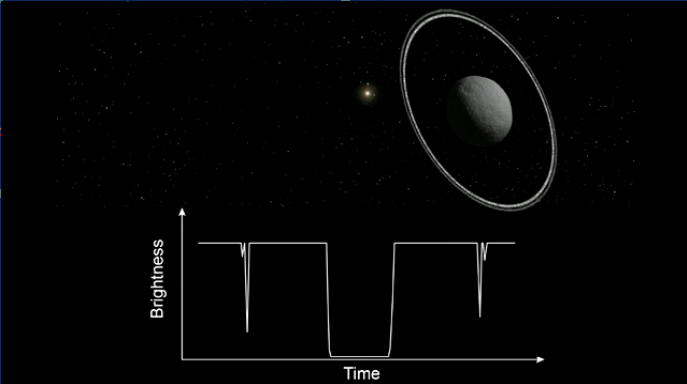
\includegraphics[scale=0.65]{pngs/curva.png}
    \caption{Representação artística de uma ocultação estelar pelo Centauro (10199)~Chariklo e seu sistema de anéis. A curva de luz esquemática (abaixo) mostra as quedas de fluxo correspondentes à passagem dos anéis e do corpo principal diante da estrela. Crédito: Lucie Maquet, 2014.}
    \label{fig:ilustracao_ocultacao}
\end{figure}

A sombra do corpo ocultante projeta-se na superfície terrestre \DIFdelbegin \DIFdel{. Cada observador, em sua posição geográfica, registra um }\DIFdelend \DIFaddbegin \DIFadd{e move-se sobre ela com velocidade \(V_S\) --- de alguns a algumas dezenas de km\,s\(^{-1}\) ---, que é a velocidade do corpo }\emph{\DIFadd{relativa ao observador}}\DIFadd{, projetada no plano do céu. Ela combina o movimento orbital do corpo, o movimento orbital da Terra (termo dominante para Centauros e TNOs, que se deslocam a poucos km\,s\(^{-1}\)) e, em menor grau, a rotação da Terra (\(\lesssim 0{,}46\)\,km\,s\(^{-1}\)). Na ocultação por Umbriel de 2020, por exemplo, \(V_S \approx 17\)\,km\,s\(^{-1}\) (Figura~\ref{fig:umbriel_painel}a). Cada observador dentro do caminho da sombra registra o }\DIFaddend intervalo de tempo durante o qual a estrela \DIFdelbegin \DIFdel{é ocultada - }\DIFdelend \DIFaddbegin \DIFadd{permanece oculta --- }\DIFaddend uma \textbf{corda} \DIFaddbegin \DIFadd{positiva ---; os instantes de imersão e emersão, projetados }\DIFaddend no plano do céu\DIFdelbegin \DIFdel{. }\DIFdelend \DIFaddbegin \DIFadd{, fornecem dois pontos do limbo do objeto. Observadores fora do caminho registram cordas negativas, que limitam até onde o limbo pode se estender. }\DIFaddend A duração e o instante central da corda dependem da posição do observador em relação ao trajeto da sombra. Vários observadores em locais diferentes produzem várias cordas; a combinação dessas cordas permite reconstruir a forma e o tamanho do corpo no plano do céu com \DIFdelbegin \DIFdel{alta }\DIFdelend precisão \DIFdelbegin \DIFdel{\mbox{%DIFAUXCMD
\citep{SORA2022}}\hskip0pt%DIFAUXCMD
. A }\DIFdelend \DIFaddbegin \DIFadd{quilométrica \mbox{%DIFAUXCMD
\citep{Ortiz2020, Umbriel2020}}\hskip0pt%DIFAUXCMD
. No entanto, a }\DIFaddend previsão de ocultações depende criticamente da precisão das posições estelares e das efemérides do corpo; a melhoria contínua desses ingredientes tem ampliado o número de eventos previstos e observados \DIFaddbegin \DIFadd{com sucesso}\DIFaddend , inserindo a técnica na era do \DIFaddbegin \DIFadd{grande volume de dados (}\DIFaddend \textit{big data}\DIFaddbegin \DIFadd{) }\DIFaddend em astronomia \citep{SORA2022, Knieling2024}. Graças à precisão astrométrica do catálogo Gaia \DIFaddbegin \DIFadd{\mbox{%DIFAUXCMD
\citep{Gaia2016, GaiaDR3}}\hskip0pt%DIFAUXCMD
}\DIFaddend , o gargalo atual para a previsão de ocultações está na qualidade das efemérides dos pequenos corpos do Sistema Solar. A Figura~\ref{fig:umbriel_painel} \DIFdelbegin \DIFdel{reúne um exemplo completo desse fluxo observacional }\DIFdelend \DIFaddbegin \DIFadd{percorre, para essa ocultação por Umbriel, o fluxo observacional completo }\DIFaddend --- do mapa de previsão da sombra e do posicionamento dos observadores aos quadros CCD e à curva de luz \DIFdelbegin \DIFdel{reduzida --- para a }\DIFdelend \DIFaddbegin \DIFadd{de }\DIFaddend ocultação \DIFdelbegin \DIFdel{por Umbriel (satélite de Urano) em 2020.
}\DIFdelend \DIFaddbegin \DIFadd{reduzida.
}\DIFaddend 

\begin{figure}[htbp]
    \centering
    \begin{minipage}[b]{0.48\textwidth}
        \centering
        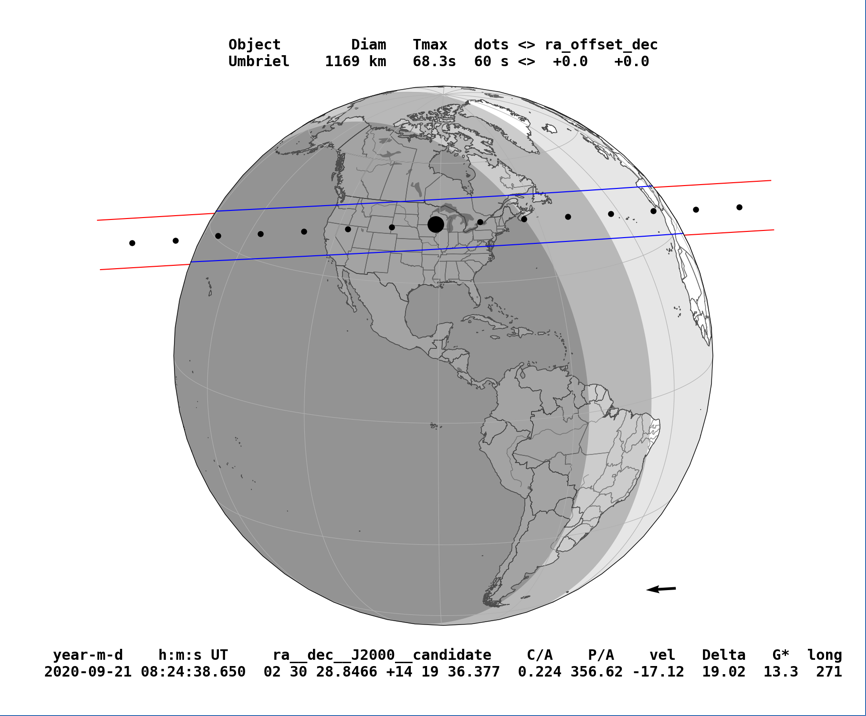
\includegraphics[width=\textwidth]{pngs/OccUmbriel_mapa.png}
        \centerline{\small (a)}
    \end{minipage}
    \hfill
    \begin{minipage}[b]{0.48\textwidth}
        \centering
        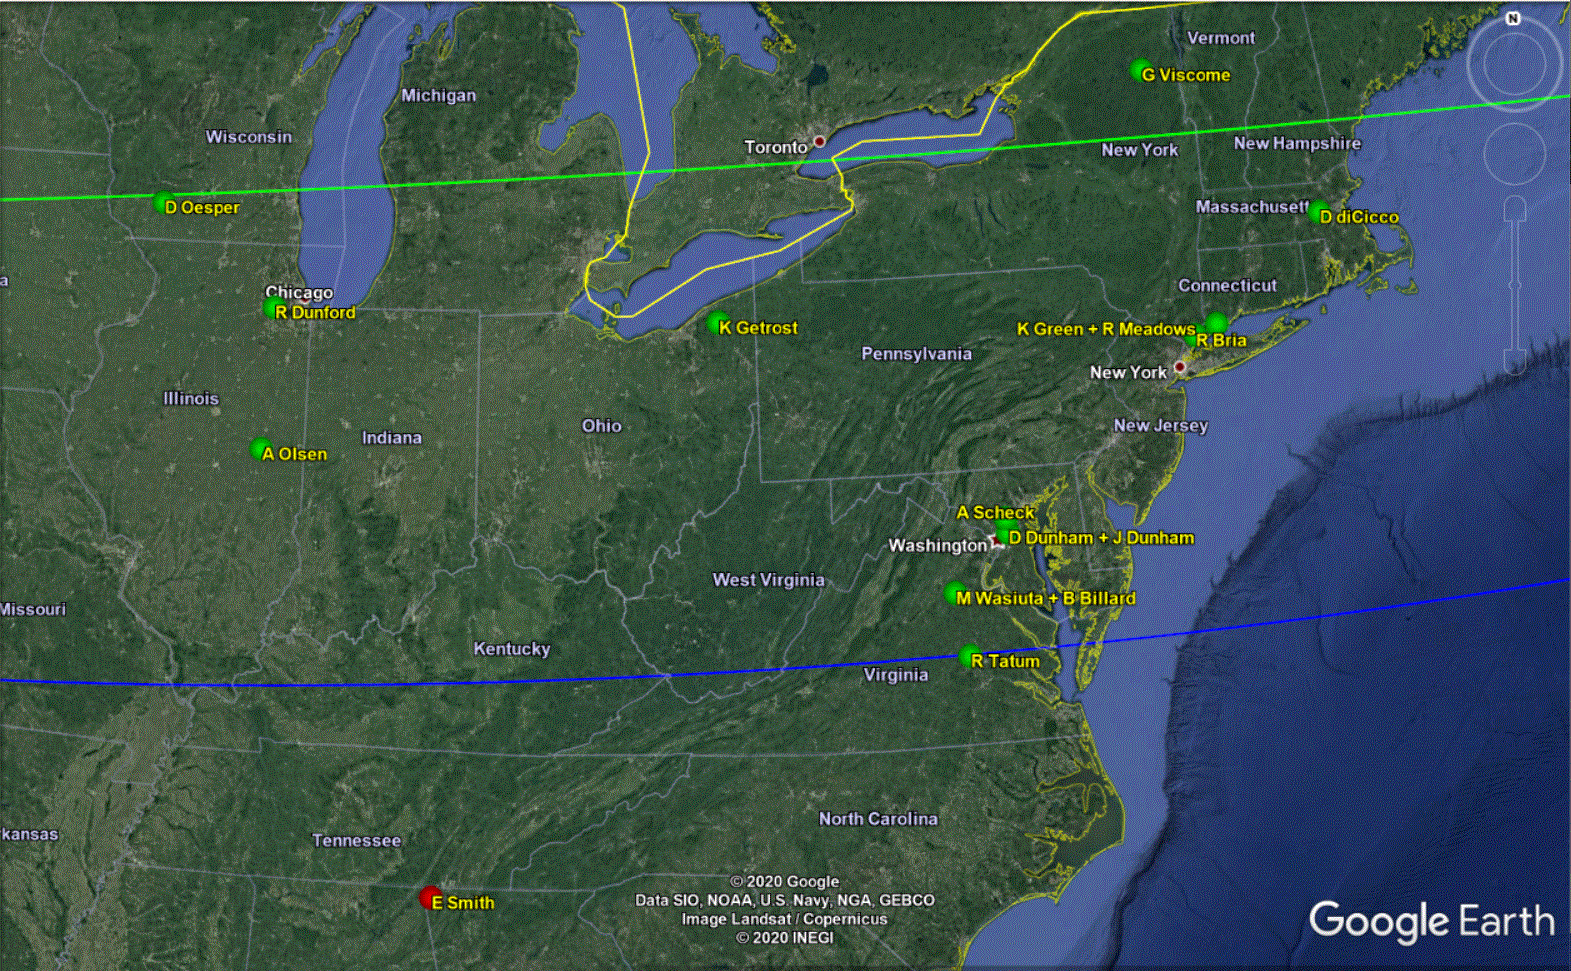
\includegraphics[width=\textwidth]{pngs/OccUmbriel_mapa2.png}
        \centerline{\small (b)}
    \end{minipage}

    \vspace{0.4cm}

    \begin{minipage}[b]{0.48\textwidth}
        \centering
        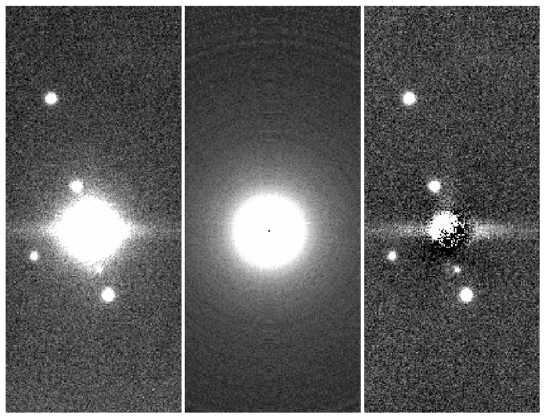
\includegraphics[width=\textwidth]{pngs/OccUmbriel_outputExemplo.png}
        \centerline{\small (c)}
    \end{minipage}
    \hfill
    \begin{minipage}[b]{0.48\textwidth}
        \centering
        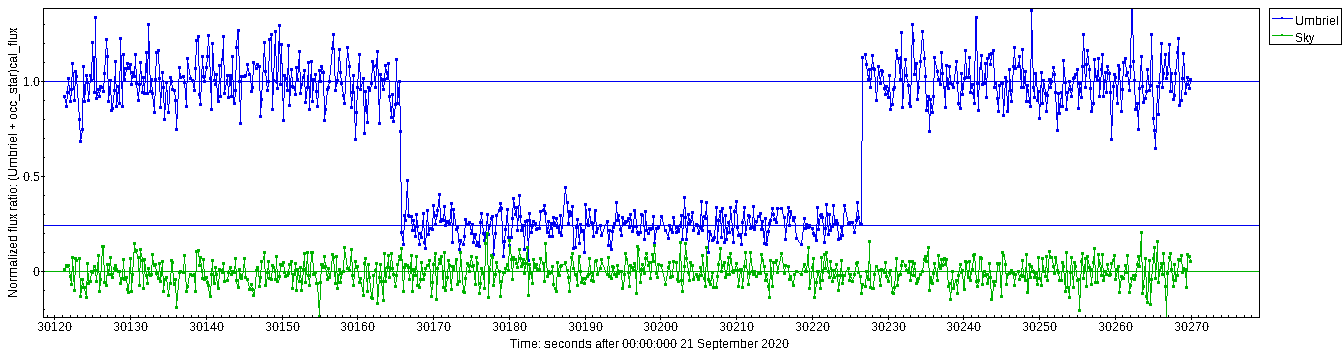
\includegraphics[width=\textwidth]{pngs/OccUmbriel_outputExemplo2.png}
        \centerline{\small (d)}
    \end{minipage}
    \caption{Exemplo completo do fluxo observacional: ocultação estelar por Umbriel (satélite de Urano), observada em 21 de setembro de \DIFdelbeginFL \DIFdelFL{2020 \mbox{%DIFAUXCMD
\citep{Umbriel2020}}\hskip0pt%DIFAUXCMD
. }\DIFdelendFL \DIFaddbeginFL \DIFaddFL{2020. }\DIFaddendFL (a)~Mapa de previsão da sombra sobre a superfície terrestre. (b)~Detalhe do posicionamento dos observadores na costa leste dos EUA (Google Earth). (c)~\DIFdelbeginFL \DIFdelFL{Exemplo de quadros }\DIFdelendFL \DIFaddbeginFL \DIFaddFL{Quadros }\DIFaddendFL CCD \DIFdelbeginFL \DIFdelFL{obtidos por }\DIFdelendFL \DIFaddbeginFL \DIFaddFL{de }\DIFaddendFL uma das estações\DIFaddbeginFL \DIFaddFL{, processados pelo PRAIA}\DIFaddendFL : \DIFdelbeginFL \DIFdelFL{são imagens como estas que alimentam os pacotes de fotometria }\DIFdelendFL \DIFaddbeginFL \DIFaddFL{imagem original }\DIFaddendFL (\DIFdelbeginFL \DIFdelFL{e.g.\ PRAIA}\DIFdelendFL \DIFaddbeginFL \DIFaddFL{esquerda}\DIFaddendFL )\DIFdelbeginFL \DIFdelFL{para a construção das curvas de luz. Neste caso}\DIFdelendFL , \DIFdelbeginFL \DIFdelFL{o brilho intenso }\DIFdelendFL \DIFaddbeginFL \DIFaddFL{modelo do halo }\DIFaddendFL de Urano \DIFdelbeginFL \DIFdelFL{exigiu }\DIFdelendFL \DIFaddbeginFL \DIFaddFL{(centro) e imagem após }\DIFaddendFL a \DIFdelbeginFL \DIFdelFL{aplicação de }\DIFdelendFL \DIFaddbeginFL \DIFaddFL{subtração por }\DIFaddendFL coronagrafia digital \DIFdelbeginFL \DIFdelFL{para viabilizar }\DIFdelendFL \DIFaddbeginFL \DIFaddFL{(direita), que viabiliza }\DIFaddendFL a fotometria \DIFdelbeginFL \DIFdelFL{precisa }\DIFdelendFL de Umbriel \DIFaddbeginFL \DIFaddFL{e da estrela}\DIFaddendFL . (d)~Curva de luz \DIFaddbeginFL \DIFaddFL{de ocultação }\DIFaddendFL resultante\DIFdelbeginFL \DIFdelFL{da redução via PRAIA}\DIFdelendFL : \DIFaddbeginFL \DIFaddFL{razão entre o }\DIFaddendFL fluxo \DIFdelbeginFL \DIFdelFL{normalizado }\DIFdelendFL \DIFaddbeginFL \DIFaddFL{da estrela somado ao }\DIFaddendFL de Umbriel \DIFaddbeginFL \DIFaddFL{e o fluxo de calibração }\DIFaddendFL (azul)\DIFaddbeginFL \DIFaddFL{, }\DIFaddendFL e \DIFdelbeginFL \DIFdelFL{ruído de }\DIFdelendFL fundo \DIFaddbeginFL \DIFaddFL{de céu }\DIFaddendFL (verde)\DIFdelbeginFL \DIFdelFL{, com a queda }\DIFdelendFL \DIFaddbeginFL \DIFaddFL{. Fonte: adaptado }\DIFaddendFL de \DIFdelbeginFL \DIFdelFL{ocultação claramente visível}\DIFdelendFL \DIFaddbeginFL \DIFaddFL{\mbox{%DIFAUXCMD
\citet{Umbriel2020}}\hskip0pt%DIFAUXCMD
}\DIFaddendFL .}
    \label{fig:umbriel_painel}
\end{figure}

A observação é tipicamente feita por telescópios amadores e profissionais, com detectores CCD ou câmeras de vídeo. A análise das imagens serve-se de \textbf{fotometria diferencial \DIFaddbegin \DIFadd{de abertura}\DIFaddend }\DIFdelbegin \DIFdel{: mede-se }\DIFdelend \DIFaddbegin \DIFadd{, em que se mede }\DIFaddend o fluxo da \DIFdelbegin \DIFdel{estrela alvo }\DIFdelend \DIFaddbegin \DIFadd{estrela-alvo }\DIFaddend em relação \DIFdelbegin \DIFdel{a }\DIFdelend \DIFaddbegin \DIFadd{ao de }\DIFaddend estrelas de referência no mesmo campo\DIFdelbegin \DIFdel{, de modo a cancelar }\DIFdelend \DIFaddbegin \DIFadd{. Como a luz de todas atravessa praticamente a mesma coluna atmosférica no mesmo instante, cancelam-se }\DIFaddend efeitos sistemáticos \DIFdelbegin \DIFdel{, tendo em conta a curta duração do evento (}\DIFdelend \DIFaddbegin \DIFadd{comuns, como }\DIFaddend extinção atmosférica, variações de transparência \DIFdelbegin \DIFdel{). O resultado da fotometria , ao longo do tempo, }\DIFdelend \DIFaddbegin \DIFadd{etc. Essa fotometria }\DIFaddend é \DIFdelbegin \DIFdel{uma }\textbf{\DIFdel{curva de luz}} %DIFAUXCMD
\DIFdel{- a série temporal do fluxo (ou }\DIFdelend \DIFaddbegin \DIFadd{usualmente feita com pacotes dedicados, como o PRAIA (}\textit{\DIFadd{Platform for Reduction of Astronomical Images Automatically}}\DIFadd{) \mbox{%DIFAUXCMD
\citep{AssafinPRAIA}}\hskip0pt%DIFAUXCMD
, que também implementa a }\textbf{\DIFadd{coronagrafia digital}}\DIFadd{: a subtração, imagem a imagem, de um modelo do halo de um objeto muito brilhante próximo ao alvo --- como Urano, no caso de Umbriel \mbox{%DIFAUXCMD
\citep{Assafin2023}}\hskip0pt%DIFAUXCMD
. A }\textbf{\DIFadd{curva de luz de ocultação}} \DIFadd{é a }\DIFaddend razão \DIFdelbegin \DIFdel{de fluxos) }\DIFdelend \DIFaddbegin \DIFadd{entre o fluxo medido na abertura da estrela-alvo e o fluxo das estrelas de referência da mesma imagem, }\DIFaddend em função do tempo. Em \DIFaddbegin \DIFadd{geral, o corpo ocultante não é resolvido da estrela: a abertura contém a soma estrela + corpo, e a luz do corpo continua presente durante a ocultação (Seção~\ref{sec:caracteristicas_curvas}). Em }\DIFaddend uma detecção \textbf{positiva}, a curva exibe um trecho de fluxo aproximadamente constante (estrela ainda não ocultada), uma queda relativamente abrupta (\DIFdelbegin \DIFdel{ingresso da estrela atrás do corpo}\DIFdelend \DIFaddbegin \DIFadd{a imersão: o corpo passa diante da estrela e o observador entra na sombra}\DIFaddend ), um patamar \DIFdelbegin \DIFdel{baixo (ocultação total ou parcial) }\DIFdelend \DIFaddbegin \DIFadd{de baixo fluxo }\DIFaddend e o retorno ao \DIFdelbegin \DIFdel{fluxo total da estrela (egresso}\DIFdelend \DIFaddbegin \DIFadd{nível inicial (a emersão}\DIFaddend ). Em uma detecção \textbf{negativa}, não há queda significativa; a curva permanece estável (ou com flutuações de ruído), e essa informação é igualmente útil\DIFdelbegin \DIFdel{para dar um limite superior ao tamanho da sombra e refinar modelos. A análise detalhada da curva (ajuste de modelos que incluem }\DIFdelend \DIFaddbegin \DIFadd{: uma corda negativa delimita até onde o limbo do corpo pode se estender naquela direção. O ajuste de uma curva sintética --- que considera o }\DIFaddend diâmetro aparente da estrela \DIFdelbegin \DIFdel{, }\DIFdelend \DIFaddbegin \DIFadd{projetado à distância do corpo, a }\DIFaddend difração de Fresnel e \DIFaddbegin \DIFadd{o }\DIFaddend tempo de exposição \DIFdelbegin \DIFdel{) }\DIFdelend \DIFaddbegin \DIFadd{usado na observação --- }\DIFaddend permite obter os instantes de imersão e emersão com \DIFdelbegin \DIFdel{alta }\DIFdelend precisão \DIFdelbegin \DIFdel{e}\DIFdelend \DIFaddbegin \DIFadd{da ordem de frações de segundo e, projetando esses instantes no plano do céu}\DIFaddend , \DIFdelbegin \DIFdel{a partir deles, }\DIFdelend as dimensões e a forma \DIFdelbegin \DIFdel{do corpo \mbox{%DIFAUXCMD
\citep{SORA2022}}\hskip0pt%DIFAUXCMD
}\DIFdelend \DIFaddbegin \DIFadd{bidimensional do objeto \mbox{%DIFAUXCMD
\citep{Ortiz2020, SORA2022}}\hskip0pt%DIFAUXCMD
}\DIFaddend .



% ---------------------------
\section{Da observação às curvas de luz: coleta e armazenamento}
\label{sec:coleta_armazenamento}

As curvas de luz utilizadas em campanhas de ocultações provêm de redes de telescópios (profissionais e amadores) que registram o fluxo da estrela alvo em cadência rápida (exposições de fração de segundo a poucos segundos, com o mínimo possível de \DIFaddbegin \DIFadd{intervalo entre imagens sucessivas --- o chamado }\DIFaddend tempo morto) para maximizar a resolução temporal e, portanto, espacial ao longo da corda. O volume de dados gerado é grande: cada observação pode produzir milhares de quadros e da ordem de gigabytes por evento \citep{Cazeneuve2023}. A redução fotométrica (extração do fluxo em cada quadro) é feita com \DIFdelbegin \DIFdel{pacotes dedicados, como o PRAIA(}\textit{\DIFdel{Package for the Reduction of Astronomical Images Automatically}}%DIFAUXCMD
\DIFdel{)}\DIFdelend \DIFaddbegin \DIFadd{o PRAIA}\DIFaddend , que automatiza a fotometria de abertura e a construção da curva de luz a partir das imagens \citep{Assafin2023}. O \DIFdelbegin \DIFdel{SORA (}\DIFdelend \textit{Stellar Occultation Reduction and Analysis} \DIFdelbegin \DIFdel{) \mbox{%DIFAUXCMD
\citep{SORA2022} }\hskip0pt%DIFAUXCMD
}\DIFdelend \DIFaddbegin \DIFadd{\mbox{%DIFAUXCMD
\citep[SORA,][]{SORA2022} }\hskip0pt%DIFAUXCMD
}\DIFaddend é utilizado na etapa de análise e redução pós-fotometria para ajuste de modelos às curvas e extração de parâmetros físicos; sua saída pode alimentar bancos de dados e catálogos (como os do Grupo do Rio\DIFaddbegin \DIFadd{, grupo de pesquisa em ocultações estelares formado por pesquisadores do Observatório Nacional e de instituições colaboradoras}\DIFaddend ). Após a redução, as curvas são armazenadas em bancos de dados ou catálogos (por exemplo, VizieR, bancos de grupos de pesquisa), em formato tabular: cada registro associa uma observação a uma série de pontos (tempo, fluxo), além de metadados (objeto ocultante, data, observador, classificação positiva/negativa quando disponível\DIFaddbegin \DIFadd{, etc.}\DIFaddend ).

Nesta dissertação, a \textit{pipeline} de detecção (Capítulo 4) parte de curvas \textbf{já reduzidas} (pós-PRAIA/pós-SORA ou equivalentes), obtidas de fontes externas (Grupo do Rio, VizieR) e inseridas em um banco de dados relacional. Ou seja, o fluxo aqui descrito começa após a etapa de redução fotométrica e análise; a estrutura do banco, o fluxo de aquisição e a normalização do fluxo são detalhados no Capítulo 4. Aqui basta destacar que as curvas de luz são o insumo central para a etapa de classificação por ML: cada curva será convertida em um vetor de características e classificada como positiva ou negativa pelos modelos descritos no Capítulo 3.

% ---------------------------
\section{\DIFdelbegin \DIFdel{Características }\DIFdelend \DIFaddbegin \DIFadd{Caracterização }\DIFaddend das curvas de luz \DIFdelbegin \DIFdel{e detecção positiva/negativa}\DIFdelend \DIFaddbegin \DIFadd{de ocultação}\DIFaddend }
\label{sec:caracteristicas_curvas}

Do ponto de vista observacional, uma curva de luz de ocultação é uma série temporal de fluxo\DIFdelbegin \DIFdel{(normalmente normalizado em relação ao }\DIFdelend \DIFaddbegin \DIFadd{, normalizada de modo que o }\DIFaddend nível fora da ocultação \DIFdelbegin \DIFdel{). }\DIFdelend \DIFaddbegin \DIFadd{(estrela + corpo) valha 1. }\DIFaddend Sua \textbf{morfologia} depende de \DIFdelbegin \DIFdel{vários }\DIFdelend fatores físicos \DIFaddbegin \DIFadd{--- razão de brilho entre o corpo e a estrela, diâmetro aparente da estrela, difração de Fresnel, velocidade da sombra e presença de atmosfera, anéis ou satélites --- e de fatores instrumentais }\DIFaddend e \DIFdelbegin \DIFdel{instrumentais}\DIFdelend \DIFaddbegin \DIFadd{atmosféricos --- tempo de exposição e tempo morto, cintilação, nuvens e qualidade da fotometria}\DIFaddend .

\textbf{Detecção positiva e negativa.} Em uma detecção positiva, a curva exibe uma queda de fluxo durante o intervalo de tempo em que o \DIFdelbegin \DIFdel{trânsito ocorre. A profundidade da queda }\DIFdelend \DIFaddbegin \DIFadd{observador }\DIFaddend está \DIFdelbegin \DIFdel{relacionada à fração do disco estelar ocultada e à geometria da corda; em ocultações centrais ou próximas do centro, a queda pode ser total (fluxo }\DIFdelend \DIFaddbegin \DIFadd{dentro da sombra. Para um corpo sem atmosfera, muito maior que a estrela projetada e que a escala de Fresnel, qualquer corda que cruze o disco bloqueia toda a luz da estrela, seja ela central ou não: a posição da corda determina a }\emph{\DIFadd{duração}} \DIFadd{da queda, e não a sua profundidade. A profundidade depende da razão entre os brilhos do corpo e da estrela, porque a luz do próprio corpo continua a ser registrada na abertura. O patamar normalizado vale
}\[
\DIFadd{F_{\mathrm{oc}} = \frac{F_{\mathrm{c}}}{F_{\star}+F_{\mathrm{c}}} = \frac{1}{1+10^{\,0{,}4\,(m_{\mathrm{c}}-m_{\star})}},
}\]
\DIFadd{em que \(F\) e \(m\) são o fluxo e a magnitude do corpo (c) e da estrela (\(\star\)). Na ocultação por Umbriel (Figura~\ref{fig:umbriel_painel}d), o patamar \(\approx 0{,}24\) corresponde a \(m_{\mathrm{c}}-m_{\star} \approx 1{,}2\)\,mag; para TNOs, em geral muito mais fracos que a estrela ocultada, o patamar fica }\DIFaddend próximo de zero\DIFdelbegin \DIFdel{no patamar)}\DIFdelend . Em uma detecção negativa, o observador está fora da sombra; a curva não apresenta queda significativa, apenas flutuações típicas de ruído fotométrico, atmosférico e instrumental. Tanto positivas quanto negativas são úteis: as primeiras fornecem cordas para o ajuste de forma e tamanho; as \DIFdelbegin \DIFdel{segundas }\DIFdelend \DIFaddbegin \DIFadd{últimas }\DIFaddend ajudam a delimitar a borda da sombra e a descartar falsos positivos \citep{SORA2022}.

\textbf{Fatores que afetam a forma da curva.} O perfil da queda (ingresso e egresso) é influenciado pelo \textbf{diâmetro aparente da estrela} à distância do corpo ocultante: estrelas cujo diâmetro angular não é desprezível nessa escala produzem, em combinação com o ciclo de integração do detector, uma transição suave entre \DIFdelbegin \DIFdel{o nível desocultado e o ocultado }\DIFdelend \DIFaddbegin \DIFadd{os níveis de fluxo desocultado e ocultado da estrela}\DIFaddend . A \textbf{difração de Fresnel} nas bordas do corpo suaviza adicionalmente as regiões de ingresso e egresso; a escala típica é da ordem de \DIFdelbegin \DIFdel{\(f = \sqrt{D\lambda/2}\)}\DIFdelend \DIFaddbegin \DIFadd{\(L_{\mathrm{F}} = \sqrt{D\lambda/2}\)}\DIFaddend , onde \(D\) é a distância entre o observador e o corpo ocultante \DIFdelbegin \DIFdel{(ou, em convenções equivalentes, a distância estrela--corpo) }\DIFdelend e \(\lambda\) o comprimento de onda \citep{Roques1987}\DIFaddbegin \DIFadd{; a distância da estrela não entra na expressão, pois ela está, para todos os efeitos, no infinito}\DIFaddend . Essa suavização faz com que os instantes de ``meia-luz'' não coincidam exatamente com o contato geométrico do limbo; exposições longas ou baixa resolução temporal podem mascarar os detalhes da difração e reduzir a precisão da extração dos tempos de imersão e emersão \citep{SORA2022}. O \textbf{tempo de exposição} converte-se em resolução espacial ao longo da corda por meio da relação \(r_t = V_S \times t_{\mathrm{exp}}\), onde \(r_t\) é a resolução espacial efetiva, \(V_S\) é a velocidade da sombra projetada na superfície terrestre e \(t_{\mathrm{exp}}\) é o tempo de exposição\DIFdelbegin \DIFdel{; }\DIFdelend \DIFaddbegin \DIFadd{. Desse modo, }\DIFaddend exposições longas \DIFdelbegin \DIFdel{podem suavizar ou mascarar }\DIFdelend \DIFaddbegin \DIFadd{suavizam ou mascaram os }\DIFaddend detalhes da difração. A rigor, a amostragem ao longo da corda é determinada pelo \textbf{ciclo completo} entre quadros \DIFaddbegin \DIFadd{sucessivos }\DIFaddend --- o tempo de exposição somado ao tempo morto\DIFdelbegin \DIFdel{de leitura (}\textit{\DIFdel{readout}}%DIFAUXCMD
\DIFdel{)}\DIFdelend : enquanto \(t_{\mathrm{exp}}\) borra cada ponto ao longo de um intervalo \(V_S\,t_{\mathrm{exp}}\), o tempo morto abre lacunas entre medidas sucessivas, de modo que um tempo morto elevado degrada a resolução efetiva mesmo com exposições curtas --- daí a busca por minimizá-lo na aquisição (Seção~\ref{sec:coleta_armazenamento}). A Figura~\ref{fig:modelo_sora} mostra como essas componentes --- difração de Fresnel, tamanho angular da estrela e ciclo de integração do detector --- se combinam no modelo de curva de luz utilizado pelo SORA \citep{SORA2022}. Em corpos com atmosfera, refração e absorção modificam o perfil da curva e permitem inferir composição e estrutura da atmosfera\DIFdelbegin \DIFdel{(}\DIFdelend \DIFaddbegin \DIFadd{, como }\DIFaddend perfis de temperatura e densidade em função da altitude \DIFdelbegin \DIFdel{) }\DIFdelend \citep{Sicardy2016}; anéis ou satélites podem produzir quedas adicionais ou assimetrias \citep{BragaRibas2014}. Para a detecção automatizada por ML, o que importa é que curvas com ocultação exibem uma queda sustentada e característica no fluxo, ao passo que curvas negativas ou com apenas ruído não exibem esse padrão; flutuações atmosféricas ou instrumentais podem, no entanto, imitar quedas pontuais, o que torna a tarefa de classificação não trivial e motiva o uso de modelos treinados e de características bem escolhidas (Capítulos 3 e 4).

\begin{figure}[htbp]
    \centering
    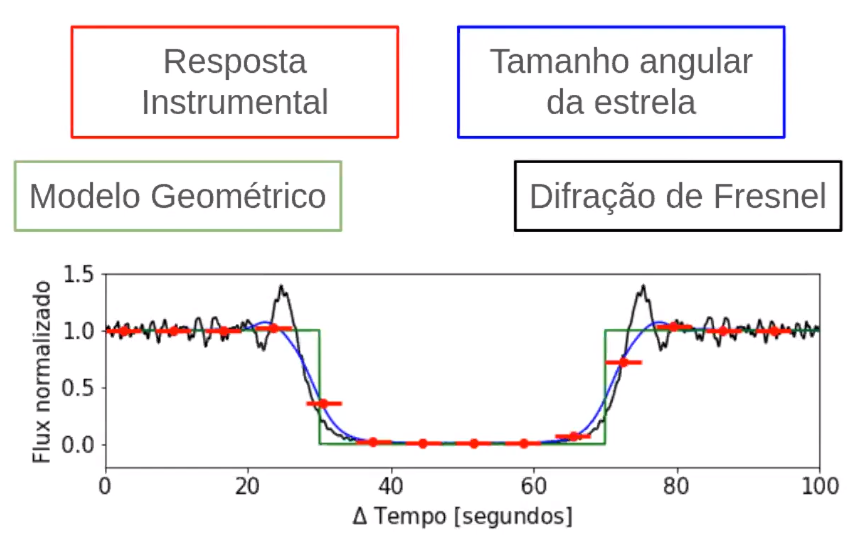
\includegraphics[width=0.55\linewidth]{pngs/ModelosSORA.png}
    \caption{Componentes do modelo de curva de luz \DIFaddbeginFL \DIFaddFL{sintética }\DIFaddendFL utilizado pelo SORA \citep{SORA2022}\DIFaddbeginFL \DIFaddFL{. Verde}\DIFaddendFL : \DIFaddbeginFL \DIFaddFL{modelo geométrico, o ponto de partida --- corpo opaco de borda nítida ocultando uma estrela pontual, sem }\DIFaddendFL difração \DIFaddbeginFL \DIFaddFL{e com amostragem instantânea. Preto: o mesmo modelo incluindo a difração }\DIFaddendFL de Fresnel\DIFdelbeginFL \DIFdelFL{(azul), tamanho }\DIFdelendFL \DIFaddbeginFL \DIFaddFL{. Azul: incluindo também o diâmetro }\DIFaddendFL angular da estrela\DIFaddbeginFL \DIFaddFL{. Traços vermelhos: resposta instrumental}\DIFaddendFL , \DIFdelbeginFL \DIFdelFL{ciclo de integração do detector e}\DIFdelendFL \DIFaddbeginFL \DIFaddFL{isto é}\DIFaddendFL , \DIFdelbeginFL \DIFdelFL{resultante da combinação dessas componentes, }\DIFdelendFL o \DIFdelbeginFL \DIFdelFL{modelo geométrico }\DIFdelendFL \DIFaddbeginFL \DIFaddFL{valor que cada exposição registraria ao integrar a curva azul durante o tempo de exposição }\DIFaddendFL (\DIFdelbeginFL \DIFdelFL{verde}\DIFdelendFL \DIFaddbeginFL \DIFaddFL{a largura de cada traço}\DIFaddendFL ). \DIFdelbeginFL \DIFdelFL{O ajuste simultâneo aos }\DIFdelendFL \DIFaddbeginFL \DIFaddFL{A curva sintética ajustada a }\DIFaddendFL dados \DIFdelbeginFL \DIFdelFL{observados }\DIFdelendFL \DIFaddbeginFL \DIFaddFL{reais combina todos esses efeitos }\DIFaddendFL (\DIFdelbeginFL \DIFdelFL{pontos vermelhos) permite determinar com precisão os instantes de imersão e emersão, necessários para }\DIFdelendFL \DIFaddbeginFL \DIFaddFL{Figura~\ref{fig:curvas_cordas}}\DIFaddendFL a\DIFdelbeginFL \DIFdelFL{reconstrução da forma do corpo}\DIFdelendFL \DIFaddbeginFL \DIFaddFL{)}\DIFaddendFL .}
    \label{fig:modelo_sora}
\end{figure} 

\textbf{Exemplo numérico: escala de Fresnel.} Para um objeto transnetuniano (TNO) a uma distância típica de $D = 40$\,UA $\approx 6{,}0 \times 10^{12}$\,m, observado no visível ($\lambda = 500$\,nm), a escala de Fresnel é
\[
\DIFdelbegin \DIFdel{f }\DIFdelend \DIFaddbegin \DIFadd{L_{\mathrm{F}} }\DIFaddend = \sqrt{\frac{D\lambda}{2}} \approx \sqrt{\frac{6{,}0 \times 10^{12} \times 5{,}0 \times 10^{-7}}{2}} \approx 1{,}2\;\text{km}.
\]
\DIFdelbegin \DIFdel{Essa escala define }\DIFdelend \DIFaddbegin \DIFadd{A difração limita }\DIFaddend a resolução \DIFdelbegin \DIFdel{espacial efetiva }\DIFdelend \DIFaddbegin \emph{\DIFadd{ao longo da corda}}\DIFadd{, isto é, }\DIFaddend na direção \DIFdelbegin \DIFdel{perpendicular à corda}\DIFdelend \DIFaddbegin \DIFadd{do movimento da sombra através do limbo}\DIFaddend : detalhes menores que \DIFdelbegin \DIFdel{$f$ }\DIFdelend \DIFaddbegin \DIFadd{$L_{\mathrm{F}}$ nessa direção }\DIFaddend são suavizados\DIFdelbegin \DIFdel{pela difração. Ainda assim, trata-se de }\DIFdelend \DIFaddbegin \DIFadd{; na direção perpendicular às cordas, a resolução é dada pelo espaçamento entre os observadores. Na prática, a resolução efetiva ao longo da corda é o maior entre três comprimentos: $L_{\mathrm{F}}$, o diâmetro aparente da estrela projetado à distância do corpo e o deslocamento da sombra durante um ciclo de aquisição. Trata-se de }\DIFaddend uma resolução da ordem \DIFdelbegin \DIFdel{de quilômetros }\DIFdelend \DIFaddbegin \DIFadd{do quilômetro na observação de objetos }\DIFaddend a dezenas de unidades astronômicas de distância -\DIFaddbegin \DIFadd{--}\DIFaddend  superior à de qualquer telescópio óptico terrestre operando por imageamento direto. É essa capacidade de resolução que torna as ocultações estelares uma ferramenta única para a caracterização de pequenos corpos do Sistema Solar.

\textbf{Relação sinal-ruído e qualidade.} A confiabilidade da detecção e da extração de parâmetros físicos depende da relação sinal-ruído (\DIFdelbegin \DIFdel{S/N}\DIFdelend \DIFaddbegin \DIFadd{SNR}\DIFaddend ) da curva. Em astronomia, muitas medições são feitas no limite da detectabilidade instrumental, onde o ruído pode produzir excursões que imitam fontes tênues; definições operacionais claras de detecção e critérios estatísticos são essenciais para interpretar os dados de forma confiável \citep{Wall2003}. \DIFdelbegin \DIFdel{S/N }\DIFdelend \DIFaddbegin \DIFadd{SNR }\DIFaddend alto favorece a identificação clara da queda e a precisão dos instantes de imersão e emersão; curvas com \DIFdelbegin \DIFdel{S/N }\DIFdelend \DIFaddbegin \DIFadd{SNR }\DIFaddend baixo são mais difíceis de classificar e mais suscetíveis a falsos positivos e negativos. Na \textit{pipeline} desta dissertação, as características extraídas de cada curva (estatísticas de fluxo, derivadas, métricas de forma, etc.) são escolhidas de forma a capturar padrões discriminativos entre curvas com e sem ocultação, mesmo na presença de ruído; o conjunto preciso de \textit{features} e o protocolo de treinamento são apresentados no Capítulo 4. A Figura~\ref{fig:curvas_cordas} ilustra, para a ocultação por Umbriel (2020), o ajuste de \DIFdelbegin \DIFdel{um modelo a uma corda observada }\DIFdelend \DIFaddbegin \DIFadd{uma curva sintética a uma das curvas de luz de ocultação observadas nessa campanha }\DIFaddend --- com os instantes de imersão e emersão \DIFdelbegin \DIFdel{marcados }\DIFdelend \DIFaddbegin \DIFadd{indicados }\DIFaddend --- e o perfil do limbo reconstruído a partir do conjunto de cordas \citep{Umbriel2020}.

\begin{figure}[htbp]
    \centering
    \begin{minipage}[b]{0.48\textwidth}
        \centering
        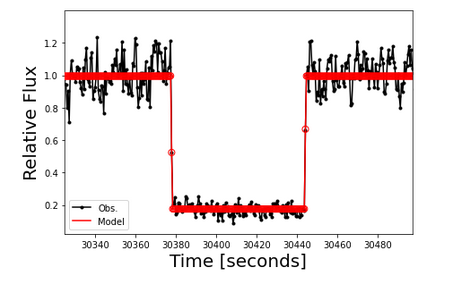
\includegraphics[width=\textwidth]{pngs/Bardecker12.png}
        \centerline{\small (a)}
    \end{minipage}
    \hfill
    \begin{minipage}[b]{0.38\textwidth}
        \centering
        \DIFdelbeginFL %DIFDELCMD < \includegraphics[scale=0.28]{Tese/pngs/LimbFitCircle.png}
%DIFDELCMD <         %%%
\DIFdelendFL \DIFaddbeginFL \includegraphics[width=\linewidth]{Tese/pngs/LimbFitCircle.png}
        \DIFaddendFL \centerline{\small (b)}
    \end{minipage}
    \caption{(a)~Curva de luz \DIFaddbeginFL \DIFaddFL{de ocultação }\DIFaddendFL observada (preto) e \DIFdelbeginFL \DIFdelFL{modelo ajustado }\DIFdelendFL \DIFaddbeginFL \DIFaddFL{curva sintética ajustada }\DIFaddendFL (vermelho) para uma das cordas da ocultação por Umbriel em 2020; os instantes de imersão e emersão \DIFdelbeginFL \DIFdelFL{, marcados por circunferências, definem a geometria }\DIFdelendFL \DIFaddbeginFL \DIFaddFL{encontram-se muito próximos dos pontos circulados nas bordas }\DIFaddendFL da \DIFdelbeginFL \DIFdelFL{corda \mbox{%DIFAUXCMD
\citep{Umbriel2020}}\hskip0pt%DIFAUXCMD
}\DIFdelendFL \DIFaddbeginFL \DIFaddFL{queda}\DIFaddendFL . (b)~Perfil do limbo de Umbriel \DIFdelbeginFL \DIFdelFL{; }\DIFdelendFL \DIFaddbeginFL \DIFaddFL{no plano do céu: }\DIFaddendFL cada linha azul \DIFdelbeginFL \DIFdelFL{(incerteza vermelho) corresponde a }\DIFdelendFL \DIFaddbeginFL \DIFaddFL{é }\DIFaddendFL uma corda \DIFaddbeginFL \DIFaddFL{positiva }\DIFaddendFL projetada\DIFdelbeginFL \DIFdelFL{no plano do céu \mbox{%DIFAUXCMD
\citep{Umbriel2020}}\hskip0pt%DIFAUXCMD
}\DIFdelendFL \DIFaddbeginFL \DIFaddFL{, com as incertezas dos extremos em vermelho}\DIFaddendFL . \DIFaddbeginFL \DIFaddFL{Fonte: adaptado de \mbox{%DIFAUXCMD
\citet{Umbriel2020}}\hskip0pt%DIFAUXCMD
.}\DIFaddendFL }
    \label{fig:curvas_cordas}
\end{figure}


% ---------------------------
\section{Considerações finais do capítulo}
\label{sec:consideracoes_cap2}

Este capítulo situou as ocultações estelares como fenômeno astronômico e as curvas de luz \DIFaddbegin \DIFadd{de ocultação }\DIFaddend como produto observacional central. \DIFdelbegin \DIFdel{Destacamos o papel da geometria da sombra }\DIFdelend \DIFaddbegin \DIFadd{Vimos que a sombra do corpo, projetada em escala 1:1 no plano do céu}\DIFaddend , \DIFdelbegin \DIFdel{das cordas e da precisão astrométrica na previsão e no aproveitamento dos eventos; a }\DIFdelend \DIFaddbegin \DIFadd{é amostrada pelas cordas dos observadores, e que é a combinação de cordas positivas e negativas que permite reconstruir forma e tamanho. Vimos também que a astrometria estelar do Gaia, ao tornar mais precisa a previsão de onde a sombra passará, aumentou o número de eventos observados com sucesso. A }\DIFaddend coleta e o armazenamento dos dados foram descritos em linhas gerais\DIFdelbegin \DIFdel{; }\DIFdelend \DIFaddbegin \DIFadd{, }\DIFaddend e foram resumidas as características observacionais das curvas. \DIFdelbegin \DIFdel{O volume crescente de dados produzidos por redes de telescópios e catálogos como o Gaia torna }\DIFdelend \DIFaddbegin \DIFadd{A combinação de previsões mais precisas, da popularização de câmeras rápidas e de baixo custo e das redes de observadores multiplicou o número de curvas de luz de ocultação a analisar e tornou }\DIFaddend penosa a triagem manual de todas \DIFdelbegin \DIFdel{as curvas de luz; essa }\DIFdelend \DIFaddbegin \DIFadd{elas. Essa }\DIFaddend escala motiva o desenvolvimento de métodos automatizados de detecção baseados em aprendizado de máquina, cujos fundamentos são apresentados no Capítulo~3 e cuja implementação é detalhada no Capítulo~4. \DIFdelbegin \DIFdel{Notadamente, nos interessam também }\DIFdelend \DIFaddbegin \DIFadd{Interessa-nos, em particular, }\DIFaddend que sejam apontados eventos tênues \DIFdelbegin \DIFdel{e }\DIFdelend que passaram despercebidos num primeiro tratamento \DIFdelbegin \DIFdel{de curvas de luz - como ocorreu , por exemplo, na descoberta dos }\DIFdelend \DIFaddbegin \DIFadd{das curvas --- como ocorreu com os }\DIFaddend anéis de Quaoar\DIFdelbegin \DIFdel{, descrito em \mbox{%DIFAUXCMD
\citep{Quaoar2023}}\hskip0pt%DIFAUXCMD
}\DIFdelend \DIFaddbegin \DIFadd{: o primeiro (Q1R) foi revelado pela revisita de dados antigos motivada por uma observação nova \mbox{%DIFAUXCMD
\citep{Morgado2023}}\hskip0pt%DIFAUXCMD
, e o segundo (Q2R) foi descrito por \mbox{%DIFAUXCMD
\citet{Quaoar2023}}\hskip0pt%DIFAUXCMD
}\DIFaddend . Um alerta confiável nesses casos é suporte para campanhas observacionais e descobertas importantes.


\chapter{Modelos e algoritmos para \DIFdelbegin \DIFdel{Machine Learning}\DIFdelend \DIFaddbegin \texorpdfstring{\textit{Machine Learning}}{Machine Learning}\DIFaddend }

% =============================================================================
% Capítulo 3 — Modelos de Machine Learning para Classificação e Agrupamento
% =============================================================================

 O Capítulo~2 mostrou que as campanhas de ocultação estelar podem produzir diversas curvas de luz, sendo número suficiente para que haja dificuldade na análise completa e minuciosa. Cada curva pode ser resumida por um conjunto de características como profundidade da queda, estatísticas de ruído, entre outros. A questão é: \emph{a partir dessa descrição numérica de uma curva, é possível decidir automaticamente se ela contém ou não uma ocultação?} Trata-se de um problema de \textbf{classificação binária}, e os métodos de \textit{Machine Learning} são as ferramentas naturais para resolvê-lo. Com isso, os objetivos deste capítulo são: definir e situar os modelos de \DIFdelbegin \DIFdel{Machine Learning }\DIFdelend \DIFaddbegin \textit{\DIFadd{Machine Learning}} \DIFaddend como ferramentas de descobertas e classificações no contexto científico; formalizar o problema de classificação (espaço de atributos, rótulos, regiões de decisão); apresentar os principais modelos utilizados na \textit{pipeline}; e, por fim, discutir algoritmos de otimização, engenharia de características, validação de modelos e os riscos de falsos resultados.

% -----------------------------------------------------------------------------
\section{Conceitos fundamentais de \DIFdelbegin \DIFdel{Machine Learning}\DIFdelend \DIFaddbegin \texorpdfstring{\textit{Machine Learning}}{Machine Learning}\DIFaddend }
\label{sec:fundamentos_ml}

\subsection{Definição e papel do aprendizado de máquina}

O \textit{Machine Learning} (ML), ou aprendizado de máquina, é uma área na qual os sistemas \DIFdelbegin \DIFdel{"aprendem" }\DIFdelend \DIFaddbegin \DIFadd{``aprendem'' }\DIFaddend a partir de dados, sem serem explicitamente programados para cada tarefa \citep{geron2019maos}. Em vez de regras fixas codificadas à mão, um algoritmo de ML é alimentado com informações e \textbf{ajusta seus próprios parâmetros} (por exemplo, coeficientes de uma combinação linear) para capturar padrões ou relações nos dados. Esse processo de ajuste é o que se chama de \textbf{treinamento}; ao final, o modelo está \DIFdelbegin \DIFdel{"treinado" }\DIFdelend \DIFaddbegin \DIFadd{``treinado'' }\DIFaddend e pode ser aplicado a novas informações. O objetivo é permitir que o sistema melhore seu desempenho à medida que mais dados ou mais iterações estejam disponíveis, especialmente em problemas sem solução analítica \DIFdelbegin \DIFdel{fechada }\DIFdelend ou com grandes volumes de dados.

No contexto científico, o ML costuma ser visto como \DIFdelbegin \DIFdel{"}\DIFdelend \DIFaddbegin \DIFadd{uma ``}\DIFaddend caixa-preta\DIFdelbegin \DIFdel{" }\DIFdelend \DIFaddbegin \DIFadd{'' }\DIFaddend que produz previsões sem explicação. Essa visão reflete usos industriais em que a precisão preditiva prevalece sobre a interpretabilidade. Em ciência, porém, o ML pode ir além: atuando como ferramenta de descoberta, revelando padrões que podem ser incorporados a uma teoria formal de causa e efeito. O papel do ML não é substituir a teoria, mas auxiliar na sua formulação, identificando os padrões que a teoria buscará explicar. Segundo \cite{lopez2020ml}, por exemplo, o uso do ML na ciência pode ser agrupado em algumas funções típicas:

\DIFaddbegin \begin{enumerate}
	\item[\DIFadd{(i)}] \DIFaddend \textbf{Sugerir a existência de algo novo:} ML pode encontrar padrões não previstos, indicando a existência de relações ainda não descobertas. Em matemática, algoritmos já auxiliaram a conjecturar teoremas que depois foram demonstrados formalmente \citep{gryak2018conjugacy}.

	\DIFaddbegin \item[\DIFadd{(ii)}] \DIFaddend \textbf{Descobrir o grau de importância das variáveis:} técnicas como \DIFaddbegin \DIFadd{a }\DIFaddend \textit{Mean Decrease Accuracy} (MDA\DIFaddbegin \DIFadd{, a queda média da acurácia}\DIFaddend ) permitem avaliar o impacto de cada variável (\textbf{\DIFdelbegin \DIFdel{feature}\DIFdelend \DIFaddbegin \textit{\DIFadd{feature}}\DIFaddend }, ou característica numérica de entrada) \DIFdelbegin \DIFdel{na }\DIFdelend \DIFaddbegin \DIFadd{sobre a saída do modelo de ML para exemplos novos --- aqui, ``}\DIFaddend predição\DIFaddbegin \DIFadd{'' é a resposta do classificador, e não a previsão de uma ocultação a partir de efemérides}\DIFaddend . A ideia é treinar o modelo, medir o desempenho (por exemplo, via acurácia), embaralhar uma variável por vez e verificar se o desempenho cai; se cair, a variável é importante \citep{liu2004comparative}. Assim, o ML identifica quais variáveis devem compor explicações teóricas, mesmo sem revelar o mecanismo causal.

	\DIFaddbegin \item[\DIFadd{(iii)}] \DIFaddend \textbf{Explorar relações de causa e efeito:} um modelo pode ser ajustado com dados nos quais um determinado efeito está ausente. Depois, quando esse efeito passa a atuar, o modelo continua produzindo previsões baseadas no cenário anterior. Se as observações reais passarem a divergir das previsões, essa diferença pode ser um indício de que o efeito alterou o sistema, sugerindo possíveis relações causais.

	\DIFaddbegin \item[\DIFadd{(iv)}] \DIFaddend \textbf{Redução e simplificação:} em dados multidimensionais, técnicas de redução de dimensionalidade \DIFdelbegin \DIFdel{— }\DIFdelend \DIFaddbegin \DIFadd{--- }\DIFaddend por exemplo, a Análise de Componentes Principais (PCA) \DIFdelbegin \DIFdel{— }\DIFdelend \DIFaddbegin \DIFadd{--- }\DIFaddend projetam os dados em um espaço de menor dimensão, tornando mais evidentes padrões, agrupamentos e relações entre observações, o que favorece a interpretação dos resultados.

	\DIFaddbegin \item[\DIFadd{(v)}] \DIFaddend \textbf{Encontrar padrões desconhecidos:} o ML pode atuar na detecção de eventos raros ou \DIFaddbegin \DIFadd{de }\DIFaddend anomalias em grandes volumes de dados -\DIFaddbegin \DIFadd{--}\DIFaddend  por exemplo, na triagem automática de \DIFdelbegin \DIFdel{ocultações estelares em levantamentos astronômicos - indicando }\DIFdelend \DIFaddbegin \DIFadd{curvas de luz de ocultação obtidas em campanhas dedicadas e por redes de observadores, como as reunidas no catálogo }\texttt{\DIFadd{B/occ/asteroid}} \DIFadd{do VizieR. A maioria dos levantamentos de imageamento de grande campo não tem tempos de exposição e cadência compatíveis com a duração de uma ocultação. O ML indica }\DIFaddend onde vale a pena investigar, mesmo sem explicar o mecanismo.
\DIFaddbegin \end{enumerate}
\DIFaddend 

Neste trabalho, o ML atua sobretudo na \DIFdelbegin \DIFdel{função de }\textbf{\DIFdel{encontrar padrões desconhecidos}} %DIFAUXCMD
\DIFdel{e }\DIFdelend \DIFaddbegin \textbf{\DIFadd{detecção de eventos}} \DIFadd{em grandes volumes de dados (triagem) e na função }\DIFaddend de \textbf{descobrir o grau de importância das variáveis} (importância das \textit{features} nos \DIFdelbegin \DIFdel{ensembles }\DIFdelend \DIFaddbegin \textit{\DIFadd{ensembles}} \DIFaddend de árvores), em apoio à decisão do pesquisador sobre quais curvas merecem análise detalhada.

\subsection{Aprendizado supervisionado versus não supervisionado}

A \DIFdelbegin \DIFdel{taxonomia }\DIFdelend \DIFaddbegin \DIFadd{classificação }\DIFaddend usual divide o ML em dois cenários, conforme a natureza dos dados:

\begin{itemize}
	\item \textbf{Supervisionado:} cada exemplo possui um rótulo (classe ou valor numérico). Tarefas típicas: classificação (rótulo discreto) e regressão (rótulo contínuo). Exemplos: filtro de \DIFdelbegin \DIFdel{spam}\DIFdelend \DIFaddbegin \textit{\DIFadd{spam}}\DIFaddend , previsão de preços \DIFaddbegin \DIFadd{e, na astronomia, classificação morfológica de galáxias e estimativa de }\textit{\DIFadd{redshift}} \DIFadd{fotométrico}\DIFaddend .
	\item \textbf{Não supervisionado:} os dados não possuem rótulos. Tarefas típicas: agrupamento (\DIFdelbegin \DIFdel{clustering}\DIFdelend \DIFaddbegin \textit{\DIFadd{clustering}}\DIFaddend ), detecção de anomalias, redução de dimensionalidade. Exemplos: segmentação de clientes, identificação de \textit{outliers} (anomalias) \DIFaddbegin \DIFadd{e, na astronomia, agrupamento de asteroides em famílias dinâmicas ou em classes espectrais e busca de objetos anômalos em grandes levantamentos \mbox{%DIFAUXCMD
\citep{Ivezic2014}}\hskip0pt%DIFAUXCMD
}\DIFaddend .
\end{itemize}

Neste trabalho, o foco é o \textbf{paradigma supervisionado}, em particular a \textbf{classificação binária}. No aprendizado supervisionado, o objetivo é encontrar uma função \(f\) que mapeie cada entrada \(\vec{x}\) (por exemplo, o vetor de características de uma curva de luz) a um rótulo \(y\) (por exemplo, \DIFdelbegin \DIFdel{"}\DIFdelend \DIFaddbegin \DIFadd{``}\DIFaddend ocultação presente\DIFdelbegin \DIFdel{" ou "ausente"}\DIFdelend \DIFaddbegin \DIFadd{'' ou ``ausente''}\DIFaddend ). Os rótulos usados no treinamento vêm da classificação já conhecida dos dados (a chamada \textbf{verdade de campo}, ou \textit{ground truth} -\DIFaddbegin \DIFadd{--}\DIFaddend  por exemplo, a análise prévia de um especialista ou o catálogo). O objetivo é que \(f\) \textbf{generalize} bem, ou seja, que erre pouco em dados novos que não foram usados no ajuste. A detecção de ocultações estelares é formulada exatamente assim: a curva de luz contém um evento de ocultação (classe positiva, \(y=1\)) ou não (classe negativa, \(y=0\)). Os classificadores (Regressão Logística, Random Forest, XGBoost, CatBoost) recebem vetores de características extraídos das curvas e produzem uma classe ou uma probabilidade de classe, permitindo triagem e priorização automáticas no fluxo da \textit{pipeline} (Capítulo 4). \DIFaddbegin \DIFadd{Neste trabalho, os classificadores foram usados por meio de bibliotecas Python de código aberto, cujas documentações pedem a citação dos trabalhos originais: }\textit{\DIFadd{scikit-learn}} \DIFadd{\mbox{%DIFAUXCMD
\citep{ScikitLearn2011}}\hskip0pt%DIFAUXCMD
, para a Regressão Logística e o Random Forest \mbox{%DIFAUXCMD
\citep{Breiman2001}}\hskip0pt%DIFAUXCMD
; XGBoost \mbox{%DIFAUXCMD
\citep{Chen2016}}\hskip0pt%DIFAUXCMD
; e CatBoost \mbox{%DIFAUXCMD
\citep{Prokhorenkova2018}}\hskip0pt%DIFAUXCMD
.
}\DIFaddend 

% -----------------------------------------------------------------------------
\section{O problema da classificação supervisionada}
\label{sec:problema_classificacao}
\label{sec:reglin_didatica}

Em notação matemática, uma amostra rotulada é representada \DIFdelbegin \DIFdel{pela tupla }\DIFdelend \DIFaddbegin \DIFadd{pelo par ordenado (ou }\textbf{\DIFadd{tupla}}\DIFadd{, isto é, uma sequência ordenada e finita de elementos) }\DIFaddend \(Z = (X, Y)\). Aqui \(X = \{\vec{x}_1, \vec{x}_2, \ldots, \vec{x}_n\}\) é o conjunto de \textbf{vetores de características}: cada \(\vec{x}_i \in \mathbb{R}^d\) é um vetor com \(d\) números que resumem, no caso deste trabalho, uma curva de luz \DIFdelbegin \DIFdel{(amplitude, }\DIFdelend \DIFaddbegin \DIFadd{de ocultação (por exemplo, a amplitude e o }\DIFaddend mínimo do fluxo suavizado\DIFdelbegin \DIFdel{, distância entre centróides, etc.}\DIFdelend ). O número \(d\) é a \DIFdelbegin \DIFdel{"}\DIFdelend \DIFaddbegin \DIFadd{``}\DIFaddend dimensionalidade'' do problema (neste \DIFdelbegin \DIFdel{caso, 14 ou }\DIFdelend \DIFaddbegin \DIFadd{trabalho, entre 11 e }\DIFaddend 28 \DIFdelbegin \DIFdel{features). O conjunto \(Y = \{y_1, y_2, \ldots, y_n\}\) }\DIFdelend \DIFaddbegin \textit{\DIFadd{features}}\DIFadd{, conforme o experimento; Capítulo~5). Dispostos como linhas, esses \(n\) vetores formam a }\textbf{\DIFadd{matriz de dados}} \DIFadd{\(\mathbf{X}\), de dimensão \(n \times d\). O conjunto \(Y =\{y_1, y_2, \ldots, y_n\}\) }\DIFaddend contém os \textbf{rótulos}: a classificação verdadeira de cada exemplo, com \(y_i \in \{0,1\}\) no caso binário (0 = sem ocultação, 1 = com ocultação).

Um \textbf{classificador} é uma função \(f \colon \mathbb{R}^d \longrightarrow \{0,1\}\) (ou, em geral, \(\{1,\ldots,c\}\) para \(c\) classes) que, dado um vetor \(\vec{x}\), prediz um rótulo \(y\). Em muitos modelos, \(f\) produz primeiro uma \textbf{probabilidade} de a classe ser positiva; a decisão final é então \DIFdelbegin \DIFdel{"positivo"~}\DIFdelend \DIFaddbegin \DIFadd{``positivo'' }\DIFaddend se essa probabilidade for maior ou igual a 50\DIFaddbegin \DIFadd{\,}\DIFaddend \%, e \DIFdelbegin \DIFdel{"negativo"~}\DIFdelend \DIFaddbegin \DIFadd{``negativo'' }\DIFaddend caso contrário. O uso do valor 0,5 é intuitivo, mas \DIFdelbegin \DIFdel{cabe frisar que }\DIFdelend é arbitrário e depende\DIFdelbegin \DIFdel{rá}\DIFdelend  do objetivo do modelo\DIFdelbegin \DIFdel{que está sendo treinado (esse limite decisório }\DIFdelend \DIFaddbegin \DIFadd{. Esse valor de corte }\DIFaddend é chamado de \DIFdelbegin \DIFdel{'threshold' nas pipelines de ML, ou $\tau$, }\DIFdelend \DIFaddbegin \textbf{\DIFadd{limiar}} \DIFadd{de decisão (em inglês, }\textit{\DIFadd{threshold}}\DIFadd{) }\DIFaddend e será \DIFdelbegin \DIFdel{melhor explorado mais adiante)}\DIFdelend \DIFaddbegin \DIFadd{denotado por $\tau$; seu ajuste é discutido na Seção~\ref{sec:threshold_tuning}}\DIFaddend . 

A função \(f\) divide o espaço \(\mathbb{R}^d\) em \textbf{regiões de decisão}: \(R_k = \{\vec{x} \in \mathbb{R}^d \mid f(\vec{x}) = k\}\). Cada região corresponde a uma classe. O objetivo do treinamento é estimar \(f\) a partir dos dados \((X,Y)\) de modo que \(f\) generalize bem para novos exemplos\DIFaddbegin \DIFadd{, }\DIFaddend não vistos \DIFaddbegin \DIFadd{durante o treinamento}\DIFaddend .

Antes de apresentar os modelos de classificação, convém fixar a ideia de treinamento como minimização de uma função de custo. O exemplo mais natural de ser explorado é a \textbf{regressão linear}. O modelo $y_i = \beta_0 + \beta_1 x_i + \epsilon_i$ descreve o comportamento médio de uma variável resposta $y$ dado $x$, com erro $\epsilon_i$ (Figura~\ref{fig:linear}).

\begin{figure}[htbp]
\begin{center}
	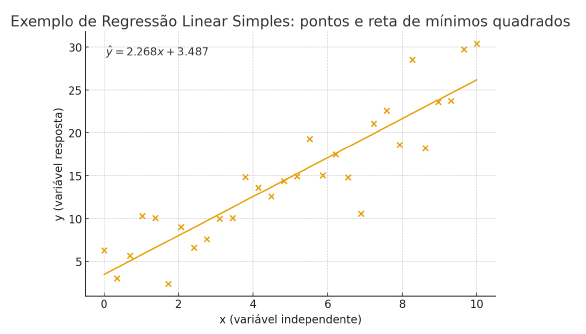
\includegraphics[scale=0.9]{pngs/exemplo_regressaoLinear.png}
\caption{Exemplo ilustrativo de regressão linear simples\DIFdelbeginFL \DIFdelFL{(}\DIFdelendFL \DIFaddbeginFL \DIFaddFL{, com }\DIFaddendFL dados genéricos, não referentes a curvas de luz de ocultação\DIFdelbeginFL \DIFdelFL{) \mbox{%DIFAUXCMD
\citep{Levada2026}}\hskip0pt%DIFAUXCMD
}\DIFdelendFL . \DIFaddbeginFL \DIFaddFL{Fonte: \mbox{%DIFAUXCMD
\citet{Levada2026}}\hskip0pt%DIFAUXCMD
.}\DIFaddendFL }
\label{fig:linear}
\end{center}
\end{figure}

Os parâmetros \DIFdelbegin \DIFdel{são }\DIFdelend \DIFaddbegin \DIFadd{podem ser }\DIFaddend estimados pelo método dos \textbf{mínimos quadrados}, que constitui o primeiro exemplo de algoritmo de otimização nesta dissertação. No caso mais simples ($\mathbb{R}^2$), o modelo é $y = \alpha + \beta x$ e a função de custo é
\[
J(\alpha,\beta) = \sum_{i=1}^{n} (y_i - \alpha - \beta x_i)^2,
\]
minimizada pela condição $\partial J / \partial \alpha = 0$, $\partial J / \partial \beta = 0$. A generalização para múltiplas variáveis ($d$ dimensões) segue naturalmente em notação vetorial. O modelo prediz \DIFdelbegin \DIFdel{$\hat{\vec{y}} = X\vec{\theta}$, com $X$ }\DIFdelend \DIFaddbegin \DIFadd{$\hat{\vec{y}} = \mathbf{X}\vec{\theta}$, com $\mathbf{X}$ }\DIFaddend a matriz de dados (cada linha é um exemplo, cada coluna uma variável) e $\vec{\theta}$ o vetor de parâmetros. A função de custo torna-se
\[
J(\vec{\theta}) = (\vec{y} - \DIFdelbegin \DIFdel{X}\DIFdelend \DIFaddbegin \DIFadd{\mathbf{X}}\DIFaddend \vec{\theta})^\top (\vec{y} - \DIFdelbegin \DIFdel{X}\DIFdelend \DIFaddbegin \DIFadd{\mathbf{X}}\DIFaddend \vec{\theta}) = \sum_{i=1}^{n} \big( y_i - \vec{\theta}^\top \vec{x}_i \big)^2.
\]
A condição de mínimo, $\nabla_{\vec{\theta}} J = \vec{0}$, fornece a \textbf{equação normal}:
\[
\DIFdelbegin \DIFdel{X}\DIFdelend \DIFaddbegin \DIFadd{\mathbf{X}}\DIFaddend ^\top (\DIFdelbegin \DIFdel{X}\DIFdelend \DIFaddbegin \DIFadd{\mathbf{X}}\DIFaddend \vec{\theta} - \vec{y}) = \vec{0} \quad \Longrightarrow \quad \vec{\theta}^* = (\DIFdelbegin \DIFdel{X}\DIFdelend \DIFaddbegin \DIFadd{\mathbf{X}}\DIFaddend ^\top \DIFdelbegin \DIFdel{X}\DIFdelend \DIFaddbegin \DIFadd{\mathbf{X}}\DIFaddend )^{-1} \DIFdelbegin \DIFdel{X}\DIFdelend \DIFaddbegin \DIFadd{\mathbf{X}}\DIFaddend ^\top \vec{y}.
\]
Após estimar $\vec{\theta}^*$, o modelo pode predizer $\vec{y}$ para novos dados de entrada \citep{geron2019maos, Levada2026}.

Apesar dos problemas de regressão servirem de excelente passo inicial para se compreender as métricas e interpretações básicas dos modelos de ML, para problemas de classificação, não usamos regressão linear diretamente -\DIFaddbegin \DIFadd{--}\DIFaddend  a solução completa desses problemas \DIFdelbegin \DIFdel{podem ser acompanhadas no capítulo }\DIFdelend \DIFaddbegin \DIFadd{pode ser acompanhada no Capítulo~}\DIFaddend 2 de \DIFdelbegin \DIFdel{\mbox{%DIFAUXCMD
\citep{Levada2026}}\hskip0pt%DIFAUXCMD
}\DIFdelend \DIFaddbegin \DIFadd{\mbox{%DIFAUXCMD
\citet{Levada2026}}\hskip0pt%DIFAUXCMD
}\DIFaddend . A \textbf{Regressão Logística} mantém a combinação linear, mas mapeia a saída ao intervalo $(0,1)$ por uma \DIFdelbegin \DIFdel{função sigmoide e }\DIFdelend \DIFaddbegin \textbf{\DIFadd{função sigmoide}}\DIFadd{, $\sigma(z)=1/(1+e^{-z})$ --- uma curva em forma de ``S'' que leva qualquer número real a um valor entre 0 e 1 (Figura~\ref{fig:sigmoide}) --- e }\DIFaddend utiliza o custo de entropia cruzada, para o qual \textbf{não existe solução \DIFdelbegin \DIFdel{fechada}\DIFdelend \DIFaddbegin \DIFadd{analítica}\DIFaddend } (o treinamento é feito por algoritmos iterativos\DIFdelbegin \DIFdel{- }\DIFdelend \DIFaddbegin \DIFadd{; }\DIFaddend Seção~\ref{sec:otimizacao}).

% -----------------------------------------------------------------------------
\section{Modelos de classificação utilizados na \DIFdelbegin \DIFdel{pipeline}\DIFdelend \DIFaddbegin \texorpdfstring{\textit{pipeline}}{pipeline}\DIFaddend }
\label{sec:modelos_classificacao}

\subsection{Regressão Logística}

A Regressão Logística é um classificador probabilístico. Similarmente à Regressão Linear, este modelo calcula uma soma ponderada das características de entrada, mas, em vez de gerar o resultado diretamente, gera a \textit{logística} (função sigmoide) desse resultado \citep{geron2019maos}. Em outras palavras, ele transforma combinações lineares de características em probabilidades válidas.

Suponha um problema de classificação no qual se deseja identificar uma ocultação em uma curva de luz a partir de uma única informação: o \textbf{tamanho da queda máxima do fluxo}. Curvas com maiores quedas possuem maior probabilidade de conter a ocultação. A \DIFdelbegin \DIFdel{figura a seguir }\DIFdelend \DIFaddbegin \DIFadd{Figura~\ref{fig:reglin_classif_ex1} }\DIFaddend ilustra a aplicação da regressão linear \DIFdelbegin \DIFdel{em dados bem comportados}\DIFdelend \DIFaddbegin \DIFadd{a oito exemplos ilustrativos --- quatro com grandes quedas de fluxo e quatro com quedas pequenas: nesse caso simples, o limiar 0,5 sobre a reta separa perfeitamente as duas classes, embora a reta produza valores fora do intervalo $[0,1]$}\DIFaddend .

\begin{figure}[htbp]
    \centering
    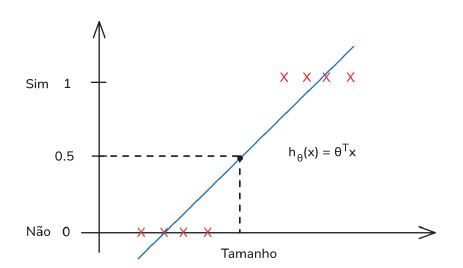
\includegraphics[width=0.5\linewidth]{pngs/regressao_linear_ex1.png}
\caption{\DIFdelbeginFL \DIFdelFL{Aplicação da regressão linear ao problema de classificação }\DIFdelendFL \DIFaddbeginFL \DIFaddFL{Classificação }\DIFaddendFL binária \DIFdelbeginFL \DIFdelFL{: a reta produz saídas fora }\DIFdelendFL \DIFaddbeginFL \DIFaddFL{(sim = 1, não = 0) em função }\DIFaddendFL do \DIFdelbeginFL \DIFdelFL{intervalo $[0,1]$ \mbox{%DIFAUXCMD
\citep{Levada2026}}\hskip0pt%DIFAUXCMD
. Nosso conjunto }\DIFdelendFL \DIFaddbeginFL \DIFaddFL{tamanho da queda }\DIFaddendFL de \DIFdelbeginFL \DIFdelFL{dados mostra quatro amostras de curvas de luz com grandes amplitudes e outras quatro com baixas amplitudes}\DIFdelendFL \DIFaddbeginFL \DIFaddFL{fluxo (marcadores)}\DIFaddendFL . \DIFdelbeginFL \DIFdelFL{Nesse exemplo simples, }\DIFdelendFL \DIFaddbeginFL \DIFaddFL{A linha tracejada indica }\DIFaddendFL o \DIFdelbeginFL \DIFdelFL{valor }\DIFdelendFL \DIFaddbeginFL \DIFaddFL{limiar }\DIFaddendFL de \DIFdelbeginFL \DIFdelFL{0}\DIFdelendFL \DIFaddbeginFL \DIFaddFL{decisão; a linha contínua}\DIFaddendFL , \DIFdelbeginFL \DIFdelFL{5 para }\DIFdelendFL o \DIFdelbeginFL \DIFdelFL{recorte }\DIFdelendFL \DIFaddbeginFL \DIFaddFL{resultado }\DIFaddendFL da \DIFdelbeginFL \DIFdelFL{reta divide perfeitamente as duas classificações}\DIFdelendFL \DIFaddbeginFL \DIFaddFL{regressão linear aplicada aos dados (ver discussão no texto)}\DIFaddendFL . \DIFaddbeginFL \DIFaddFL{Fonte: adaptado de \mbox{%DIFAUXCMD
\citet{Levada2026}}\hskip0pt%DIFAUXCMD
.}\DIFaddendFL }
    \label{fig:reglin_classif_ex1}
\end{figure}

Nesse caso, teríamos infinitos valores sob uma reta para a variável de saída. \DIFdelbegin \DIFdel{Notadamente, a }\DIFdelend \DIFaddbegin \DIFadd{A }\DIFaddend solução mais intuitiva seria considerar um limiar simples na metade da reta. No entanto, suponha que, no mesmo conjunto de dados, tivéssemos um elemento \textit{outlier}, uma anomalia. A Figura~\ref{fig:reglin_classif_ex2} ilustra a situação: \DIFaddbegin \DIFadd{a curva discrepante tem amplitude muito diferente das demais (por exemplo, por falta de normalização), a reta se desloca e }\DIFaddend o limiar que antes funcionava deixa de ser útil, pois agora a metade da reta passa a considerar um ponto positivo como negativo ao mesmo tempo que \DIFdelbegin \DIFdel{varios }\DIFdelend \DIFaddbegin \DIFadd{vários }\DIFaddend pontos positivos ficam \DIFdelbegin \DIFdel{proximos }\DIFdelend \DIFaddbegin \DIFadd{próximos }\DIFaddend do limiar de decisão (e apenas o \DIFdelbegin \DIFdel{outlier }\DIFdelend \DIFaddbegin \textit{\DIFadd{outlier}} \DIFaddend se encontra confortavelmente longe das curvas consideradas negativas), gerando dúvida para o analista que estuda os dados.

\begin{figure}[htbp]
    \centering
    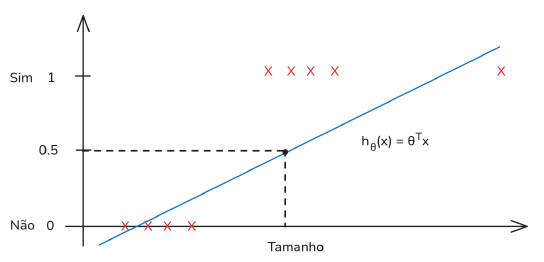
\includegraphics[width=0.5\linewidth]{pngs/regressao_linear_ex2.png}
    \caption{\DIFdelbeginFL \DIFdelFL{O mesmo problema anterior}\DIFdelendFL \DIFaddbeginFL \DIFaddFL{Como na Figura~\ref{fig:reglin_classif_ex1}}\DIFaddendFL , \DIFdelbeginFL \DIFdelFL{mas }\DIFdelendFL com a adição de um \DIFaddbeginFL \DIFaddFL{ponto discrepante (}\DIFaddendFL \textit{outlier}\DIFaddbeginFL \DIFaddFL{)}\DIFaddendFL . \DIFdelbeginFL \DIFdelFL{Uma das curvas possui tamanho }\DIFdelendFL \DIFaddbeginFL \DIFaddFL{Fonte: adaptado }\DIFaddendFL de \DIFdelbeginFL \DIFdelFL{amplitude muito diferente da escala normal, possivelmente resultado da falta de normalização}\DIFdelendFL \DIFaddbeginFL \DIFaddFL{\mbox{%DIFAUXCMD
\citet{Levada2026}}\hskip0pt%DIFAUXCMD
}\DIFaddendFL .\DIFdelbeginFL \DIFdelFL{Veja como a reta de regressão se desloca e o limiar 0,5 passa a classificar incorretamente \mbox{%DIFAUXCMD
\citep{Levada2026}}\hskip0pt%DIFAUXCMD
.}\DIFdelendFL }
    \label{fig:reglin_classif_ex2}
\end{figure}

\DIFdelbegin \DIFdel{O que podemos ver é }\DIFdelend \DIFaddbegin \DIFadd{Observa-se que }\DIFaddend a reta de regressão pode sofrer alterações significativas com a inclusão de novos pontos, evidenciando sua sensibilidade aos dados observados. Além disso, a regressão linear pode gerar valores fora do intervalo [0,1], incompatíveis com a interpretação probabilística. Dessa forma, sua sensibilidade a \DIFdelbegin \DIFdel{outliers }\DIFdelend \DIFaddbegin \textit{\DIFadd{outliers}} \DIFaddend e a ausência de uma saída naturalmente probabilística fazem da regressão linear uma abordagem inadequada para \DIFaddbegin \DIFadd{as }\DIFaddend tarefas de classificação \DIFaddbegin \DIFadd{necessárias a este trabalho}\DIFaddend .

\DIFdelbegin \DIFdel{Nesse sentido}\DIFdelend \DIFaddbegin \DIFadd{Mais adequada a esse fim}\DIFaddend , a regressão logística funciona\DIFdelbegin \DIFdel{rá}\DIFdelend  de forma similar a\DIFaddbegin \DIFadd{os}\DIFaddend  modelos lineares (saída contínua), mas \DIFdelbegin \DIFdel{será adaptado}\DIFdelend \DIFaddbegin \DIFadd{é adaptada ao nosso problema}\DIFaddend . O primeiro ponto \DIFdelbegin \DIFdel{será }\DIFdelend \DIFaddbegin \DIFadd{de adaptação é }\DIFaddend a interpretação probabilística: a combinação linear \(\vec{\theta}^\top \vec{x}\) será mapeada pela logística ao intervalo \((0,1)\), permitindo a interpretação como a probabilidade da classe ser positiva \citep{Levada2026}. 

Em notação vetorial, seja \(\vec{\theta}\) o vetor de parâmetros  e \(\vec{x}\) o vetor de atributos; a probabilidade predita é
\[
\hat{p} = h_{\vec{\theta}}(\vec{x}) = \sigma(\vec{\theta}^\top \vec{x}) = \frac{1}{1 + e^{-\vec{\theta}^\top \vec{x}}}.
\]
A decisão é: classe 1 se \(\hat{p} \geq 0{,}5\), caso contrário classe 0. Isso \DIFdelbegin \DIFdel{pois }\DIFdelend \DIFaddbegin \DIFadd{porque }\DIFaddend a saída \DIFdelbegin \DIFdel{continuará continua , mas dessa vez limitada entre 0 e 1. Vale lembrar, também, }\DIFdelend \DIFaddbegin \DIFadd{continua sendo contínua, mas agora limitada ao intervalo $(0,1)$. Ressalte-se }\DIFaddend que o valor de 0,5 pode ser alterado a depender da calibração do modelo, como discutido no início do capítulo. 

O segundo ponto \DIFdelbegin \DIFdel{a ser adaptado será quanto ao treinamento. Nesse sentido, }\DIFdelend \DIFaddbegin \DIFadd{de adaptação refere-se ao treinamento: }\DIFaddend passa-se a utilizar outra função de custo \DIFdelbegin \DIFdel{ao invés dos mínimo quadrados: }\DIFdelend \DIFaddbegin \DIFadd{em vez dos mínimos quadrados, }\DIFaddend a \textbf{entropia cruzada} (ou \textit{log loss}). Essa medida penaliza predições distantes do rótulo real. Por exemplo, se temos uma curva positiva (ocultação presente), e o modelo prediz uma probabilidade baixa de haver ocultação, o custo deverá ser alto. 

\[
loss = - [y \log{p} + (1-y) \log{(1-p)}]
\] onde p é a probabilidade prevista pelo modelo e a perda (loss) deverá ser aplicada a um único ponto. Ou seja, para um conjunto de \DIFdelbegin \DIFdel{\(m\) }\DIFdelend \DIFaddbegin \DIFadd{\(n\) }\DIFaddend exemplos, com rótulos \(y^{(i)} \in \{0,1\}\) e probabilidades preditas \(\hat{p}^{(i)}\), a função é
\begin{equation}
J(\vec{\theta}) = -\DIFdelbegin \DIFdel{\frac{1}{m} }\DIFdelend \DIFaddbegin \DIFadd{\frac{1}{n} }\DIFaddend \sum_{i=1}\DIFdelbegin \DIFdel{^{m} }\DIFdelend \DIFaddbegin \DIFadd{^{n} }\DIFaddend \left[ y^{(i)} \log(\hat{p}^{(i)}) + (1 - y^{(i)}) \log(1 - \hat{p}^{(i)}) \right].
\end{equation}


A minimização de \(J(\vec{\theta})\) é equivalente à maximização da log-verossimilhança (MLE), de modo que os parâmetros estimados são estatisticamente ótimos sob o modelo probabilístico assumido \citep{geron2019maos, Levada2026}. O ajuste é \DIFdelbegin \DIFdel{realizado por gradiente descendente(veremos mais detalhes sobre os algoritmos de otimização na }\DIFdelend \DIFaddbegin \DIFadd{iterativo. O mecanismo é ilustrado a seguir com o gradiente descendente, por ser o esquema mais intuitivo; a implementação usada neste trabalho (}\textit{\DIFadd{scikit-learn}}\DIFadd{), porém, emprega o método quasi-Newton L-BFGS (}\DIFaddend Seção~\ref{sec:otimizacao}). O gradiente de \(J\) em relação a \(\vec{\theta}\) pode ser escrito na forma vetorial
\[
\nabla_{\vec{\theta}} J(\vec{\theta}) = \DIFdelbegin \DIFdel{\frac{1}{m} X}\DIFdelend \DIFaddbegin \DIFadd{\frac{1}{n} \mathbf{X}}\DIFaddend ^\top \big( \sigma(\DIFdelbegin \DIFdel{X}\DIFdelend \DIFaddbegin \DIFadd{\mathbf{X}}\DIFaddend \vec{\theta}) - \vec{y} \big),
\]
onde \DIFdelbegin \DIFdel{\(X\) }\DIFdelend \DIFaddbegin \DIFadd{\(\mathbf{X}\) }\DIFaddend é a matriz de dados e \(\vec{y}\) o vetor de rótulos. A atualização dos parâmetros em cada iteração segue a \textbf{direção oposta ao gradiente} (direção de maior descida do custo), com passo controlado pela \textbf{taxa de aprendizado} \(\eta\) (análogo ao passo de um método numérico de minimização). Trata-se, portanto, de uma medida sobre o quão distante da realidade estão as previsões do modelo.

\vspace{0.3cm}
\noindent\textbf{Exemplo numérico: uma iteração do gradiente descendente.}
Para tornar o mecanismo concreto, considere \DIFdelbegin \DIFdel{$m = 4$ }\DIFdelend \DIFaddbegin \DIFadd{$n = 4$ }\DIFaddend curvas com uma única \DIFdelbegin \DIFdel{feature }\DIFdelend \DIFaddbegin \textit{\DIFadd{feature}} \DIFaddend $x$ (amplitude da queda de fluxo, normalizada entre 0 e 1) e rótulos $y$ (0 = sem ocultação, 1 = com ocultação):

\begin{table}[htbp]
\centering
\small
\begin{tabular}{cccc}
\hline
Curva & $x$ & $y$ & $\hat{p}$ (inicial) \\
\hline
1 & 0{,}2 & 0 & 0{,}50 \\
2 & 0{,}4 & 0 & 0{,}50 \\
3 & 0{,}7 & 1 & 0{,}50 \\
4 & 0{,}9 & 1 & 0{,}50 \\
\hline
\end{tabular}
\caption{Dados do exemplo numérico da Regressão Logística (valores ilustrativos).}
\label{tab:exemplo_logistica}
\end{table}

Inicializamos $\theta_0 = 0$ e $\theta_1 = 0$. Como $\sigma(0) = 0{,}5$, todas as curvas recebem probabilidade $\hat{p} = 0{,}5$ e o custo inicial é $J = -\log(0{,}5) \approx 0{,}693$. Os gradientes são $\partial J / \partial \theta_0 = \frac{1}{4}\sum_i (\hat{p}_i - y_i) = 0$ e \DIFdelbegin \DIFdel{$\partial J / \partial \theta_1 = \frac{1}{4}\sum_i (\hat{p}_i - y_i)\,x_i = -0{,}15$}\DIFdelend \DIFaddbegin \DIFadd{$\partial J / \partial \theta_1 = \frac{1}{4}\sum_i (\hat{p}_i - y_i)\,x_i = \frac{1}{4}(0{,}1 + 0{,}2 - 0{,}35 - 0{,}45) = -0{,}125$}\DIFaddend . Com taxa de aprendizado $\eta = 1{,}0$, a atualização dá \DIFdelbegin \DIFdel{$\theta_1 \leftarrow 0 - 1{,}0 \times (-0{,}15) = 0{,}15$}\DIFdelend \DIFaddbegin \DIFadd{$\theta_1 \leftarrow 0 - 1{,}0 \times (-0{,}125) = 0{,}125$}\DIFaddend . Recalculando as probabilidades com o novo $\theta_1$, obtemos \DIFdelbegin \DIFdel{$\hat{p}_1 = \sigma(0{,}03) \approx 0{,}507$, $\hat{p}_2 \approx 0{,}515$, $\hat{p}_3 \approx 0{,}526$ e $\hat{p}_4 \approx 0{,}534$}\DIFdelend \DIFaddbegin \DIFadd{$\hat{p}_1 = \sigma(0{,}025) \approx 0{,}506$, $\hat{p}_2 \approx 0{,}512$, $\hat{p}_3 \approx 0{,}522$ e $\hat{p}_4 \approx 0{,}528$}\DIFaddend . O custo cai para \DIFdelbegin \DIFdel{$J \approx 0{,}685$}\DIFdelend \DIFaddbegin \DIFadd{$J \approx 0{,}678$}\DIFaddend . Uma única iteração já empurrou as probabilidades na direção correta: as curvas com maior amplitude (3 e 4, positivas) receberam $\hat{p}$ ligeiramente maior que as negativas. Após centenas de iterações, a separação se consolida \DIFdelbegin \DIFdel{.
}\DIFdelend \DIFaddbegin \DIFadd{e o custo diminui continuamente. Como esses quatro pontos são linearmente separáveis (todo $x \le 0{,}4$ é negativo e todo $x \ge 0{,}7$ é positivo), sem regularização o custo só tende a zero no limite $|\theta_1| \to \infty$: não existe mínimo finito. Essa é uma das motivações para a regularização apresentada a seguir.
}\DIFaddend \vspace{0.3cm}

Sem nenhuma restrição, a Regressão Logística é livre para atribuir pesos enormes a qualquer \DIFdelbegin \DIFdel{feature }\DIFdelend \DIFaddbegin \textit{\DIFadd{feature}} \DIFaddend --- inclusive ao ruído. Se uma curva de treino por acaso tem um pico espúrio que coincide com a classe positiva, o modelo pode atribuir peso grande a essa flutuação; na hora de classificar curvas novas, esse peso exagerado prejudica a predição. Esse é o problema do \textbf{sobreajuste} (\DIFdelbegin \DIFdel{overfitting}\DIFdelend \DIFaddbegin \textit{\DIFadd{overfitting}}\DIFaddend , discutido em detalhe na Seção~\ref{sec:overfitting}): o modelo ``decorou'' particularidades do treino em vez de aprender o padrão geral.

A solução é a \textbf{regularização}: impor um custo adicional aos pesos grandes, forçando o modelo a manter coeficientes moderados e a distribuir a ``explicação'' entre múltiplas \textit{features} em vez de apostar tudo em uma \citep{geron2019maos, Levada2026}. As três formas principais são:

\begin{itemize}
	\item \textbf{Ridge (\(\ell_2\)):} adiciona ao custo o termo \(\frac{\alpha}{2} \sum_j \theta_j^2\). Os coeficientes são \textit{encolhidos} em direção a zero, mas raramente se anulam -\DIFaddbegin \DIFadd{--}\DIFaddend  todos os atributos permanecem no modelo. Funciona bem com \textit{features} correlacionadas, reduzindo o sobreajuste sem descartar características.

	\item \textbf{Lasso (\(\ell_1\)):} adiciona \(\alpha \sum_j |\theta_j|\). Tende a \textbf{zerar} coeficientes de atributos irrelevantes, atuando como seleção automática de variáveis. Em contrapartida, pode comportar-se de forma errática com muitas variáveis correlacionadas (tendendo a escolher apenas uma) ou quando o número de variáveis supera o de instâncias. A função de custo não é diferenciável em \(\theta_j = 0\) (algoritmos de otimização não sabem a direção do próximo passo), exigindo subgradientes na otimização.

	\item \textbf{Elastic Net:} combina as penalidades Ridge e Lasso com uma taxa de mistura, unindo os benefícios de ambas. É recomendado quando há muitas variáveis correlacionadas.
\end{itemize}

Existe uma interpretação elegante dessas penalidades do ponto de vista bayesiano (Estimativa MAP --- \textit{Maximum A Posteriori}). Regularizar equivale a assumir uma crença prévia (\textit{prior}) sobre os valores dos coeficientes do modelo \emph{antes} de ver os dados. No Ridge, essa crença é uma \textbf{distribuição Gaussiana} centrada em zero: acredita-se que os pesos são provavelmente pequenos, mas não necessariamente nulos --- as caudas suaves da Gaussiana permitem valores moderados (Figura~\ref{fig:gaussLaplace}). No Lasso, a crença é uma \textbf{distribuição de Laplace}, que tem um pico afiado em zero: acredita-se que muitos pesos \emph{são} zero, e apenas alguns poucos são relevantes --- daí o efeito de seleção automática de variáveis \citep{geron2019maos, Levada2026}.

O hiperparâmetro \(\alpha\) (ou \(C = 1/\alpha\)) controla a força da penalização: \(\alpha\) grande significa uma crença prévia forte de que os pesos devem ser pequenos; \(\alpha\) pequeno deixa o modelo mais livre. \DIFdelbegin \DIFdel{A }\DIFdelend \DIFaddbegin \DIFadd{Em geral, a }\DIFaddend escolha de \(\alpha\) é feita por \textbf{validação cruzada}: treina-se o modelo com diferentes valores de \(\alpha\) e seleciona-se aquele de melhor desempenho médio nas partições de validação \DIFdelbegin \DIFdel{(as }\DIFdelend \DIFaddbegin \DIFadd{\mbox{%DIFAUXCMD
\citep{geron2019maos}}\hskip0pt%DIFAUXCMD
, as chamadas }\DIFaddend \emph{dobras} \DIFdelbegin \DIFdel{, ou }\DIFdelend \DIFaddbegin \DIFadd{(}\DIFaddend \textit{folds}\DIFaddbegin \DIFadd{)}\DIFaddend , definidas na Seção~\ref{sec:validacao_modelos}\DIFdelbegin \DIFdel{) \mbox{%DIFAUXCMD
\citep{geron2019maos}}\hskip0pt%DIFAUXCMD
}\DIFdelend .

É essencial \textbf{escalonar} as \textit{features} (\DIFdelbegin \DIFdel{e.g.\ StandardScaler}\DIFdelend \DIFaddbegin \DIFadd{por exemplo, com o }\texttt{\DIFadd{StandardScaler}} \DIFadd{do }\textit{\DIFadd{scikit-learn}}\DIFaddend ) antes de aplicar Ridge ou Lasso, pois ambas as penalidades são sensíveis à escala dos dados\DIFdelbegin \DIFdel{: }\DIFdelend \DIFaddbegin \DIFadd{. Por exemplo, }\DIFaddend um atributo medido em quilômetros terá coeficiente numericamente muito diferente do mesmo atributo medido em metros, e a penalização tratará ambos de forma desigual. Nesta dissertação, utiliza-se \DIFdelbegin \DIFdel{Ridge ou Lasso na Regressão Logística, conforme documentado no }\DIFdelend \DIFaddbegin \DIFadd{apenas a penalidade Ridge ($\ell_2$), com $C = 1$ (valor padrão do }\textit{\DIFadd{scikit-learn}}\DIFadd{, sem busca de hiperparâmetros), conforme o }\DIFaddend Apêndice~\ref{ap:hiperparametros}.

\begin{figure}[!h]
    \centering
    \includegraphics[width=0.5\linewidth]{Tese/pngs/Comparison-of-Gaussian-and-Laplace-distributions.png}
    \caption{Comparação entre as distribuições Gaussiana e de Laplace, que correspondem aos priors assumidos sobre os parâmetros na interpretação bayesiana das regularizações Ridge e Lasso, respectivamente.}
    \label{fig:gaussLaplace}
\end{figure}


A Regressão Logística serve de base conceitual para entender classificadores probabilísticos e foi também treinada e avaliada na \textit{pipeline} desta dissertação, junto com os demais modelos (Random Forest, XGBoost, CatBoost), que tipicamente oferecem melhor desempenho em dados tabulares e fornecem importância de variáveis. A função sigmoide \(\sigma(z) = 1/(1+e^{-z})\) está ilustrada na Figura~\ref{fig:sigmoide}.

\begin{figure}[htbp]
\begin{center}
	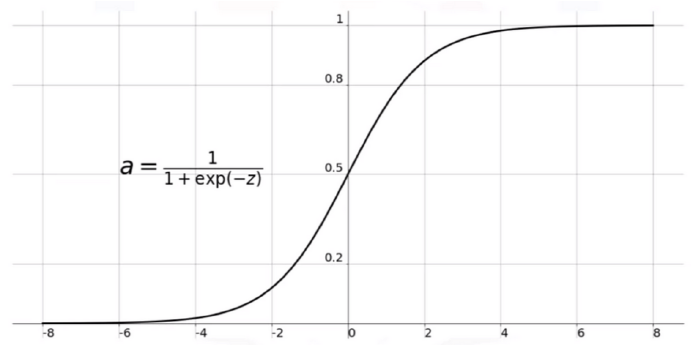
\includegraphics[scale=0.85]{pngs/sigmoide.png}
\caption{Função sigmoide \(\sigma(z) = 1/(1+e^{-z})\).}
\label{fig:sigmoide}
\end{center}
\end{figure}

\subsection{Árvores de decisão e critérios de impureza}

Os modelos Random Forest, XGBoost e CatBoost são baseados em \textbf{árvores de decisão}. Uma árvore de decisão é um classificador que funciona como um fluxograma: em cada \DIFdelbegin \DIFdel{"}\DIFdelend \DIFaddbegin \DIFadd{``}\DIFaddend nó\DIFdelbegin \DIFdel{"~ }\DIFdelend \DIFaddbegin \DIFadd{'' }\DIFaddend pergunta-se o valor de uma das características (por exemplo, \DIFdelbegin \DIFdel{"}\DIFdelend \DIFaddbegin \DIFadd{``}\DIFaddend o mínimo do fluxo suavizado é menor que 0,85?\DIFdelbegin \DIFdel{"}\DIFdelend \DIFaddbegin \DIFadd{''}\DIFaddend ); conforme a resposta, segue-se por um dos dois ramos até um novo nó ou até uma \DIFdelbegin \DIFdel{"folha"}\DIFdelend \DIFaddbegin \DIFadd{``folha''}\DIFaddend , que devolve a classe predita. O espaço de entradas (vetores de características) fica assim particionado em regiões (\DIFaddbegin \DIFadd{chamadas de }\DIFaddend hiper-retângulos), cada uma associada a uma classe \citep{Levada2026}. Uma das maiores vantagens \DIFaddbegin \DIFadd{desses modelos }\DIFaddend é a \textbf{interpretabilidade}: as regras podem ser lidas e aplicadas manualmente, em contraste com modelos opacos como redes neurais. \DIFdelbegin \DIFdel{O }\DIFdelend \DIFaddbegin \DIFadd{A biblioteca Python }\DIFaddend \textit{scikit-learn} \citep{ScikitLearn2011}\DIFaddbegin \DIFadd{, usada neste trabalho na Regressão Logística, no Random Forest, no K-means, na imputação, na padronização e no cálculo das métricas, }\DIFaddend utiliza o algoritmo \textbf{CART} (\textit{Classification and Regression Trees}), que produz árvores binárias e escolhe, em cada nó, a divisão que maximiza a pureza dos nós filhos \citep{geron2019maos}. Os dois critérios de impureza mais usados para classificação são o \textbf{coeficiente de Gini} e a \textbf{entropia}. Para um nó \(i\) com proporções \(p_{i,k}\) de exemplos na classe \(k\) (com \(k=1,\ldots,c\) classes):
\begin{equation}
G_i = 1 - \sum_{k=1}^{c} p_{i,k}^2, \qquad
H_i = -\sum_{k=1}^{c} p_{i,k} \log_2(p_{i,k}) \quad (\text{convenção } 0\log 0 = 0).
\end{equation}
Nessas expressões, \(G_i\) é o coeficiente de Gini e \(H_i\) é a \textbf{entropia} do nó \(i\): ambos medem a impureza, ou seja, o quanto as classes estão misturadas naquele nó. Os dois valem zero quando o nó é puro (todos os exemplos pertencem a uma única classe) e crescem à medida que as classes ficam mais equilibradas entre si.

O Gini tende a isolar a classe mais frequente; a entropia tende a produzir árvores mais equilibradas. A divisão é feita de modo a maximizar a redução da impureza (ganho de informação). Árvores de decisão são instáveis e sensíveis a pequenas variações nos dados; sem restrições, tendem ao sobreajuste. Para regularizar, utilizam-se critérios de parada como \DIFaddbegin \DIFadd{a }\DIFaddend profundidade máxima \DIFdelbegin \DIFdel{(}\textit{\DIFdel{max\_depth}}%DIFAUXCMD
\DIFdel{) e }\DIFdelend \DIFaddbegin \DIFadd{e o }\DIFaddend número mínimo de amostras por nó ou por folha \DIFdelbegin \DIFdel{(}\textit{\DIFdel{min\_samples\_leaf}}%DIFAUXCMD
\DIFdel{) \mbox{%DIFAUXCMD
\citep{geron2019maos} }\hskip0pt%DIFAUXCMD
}\DIFdelend \DIFaddbegin \DIFadd{\mbox{%DIFAUXCMD
\citep{geron2019maos} }\hskip0pt%DIFAUXCMD
--- no }\textit{\DIFadd{scikit-learn}}\DIFadd{, os hiperparâmetros }\texttt{\DIFadd{max\_depth}} \DIFadd{e }\texttt{\DIFadd{min\_samples\_leaf}}\DIFaddend . A \textbf{poda} (\textit{pruning}) pode ser aplicada após o crescimento completo, removendo ramos que não contribuem significativamente para a capacidade preditiva \citep{Levada2026}.

\vspace{0.3cm}
\noindent\textbf{Exemplo numérico: redução de impureza de Gini em uma divisão.}
Considere um nó contendo $8$ curvas de luz de treino, sendo $4$ positivas (com ocultação) e $4$ negativas. Como as classes estão perfeitamente misturadas, a impureza é máxima para o caso binário:
\[
G_{\text{nó}} = 1 - \left[\left(\tfrac{4}{8}\right)^2 + \left(\tfrac{4}{8}\right)^2\right] = 1 - 0{,}5 = 0{,}5.
\]
A árvore testa então uma divisão candidata --- por exemplo, ``profundidade da queda $> 0{,}5$?'' --- que separa as $8$ curvas em dois nós-filhos:
\begin{itemize}
	\item \textbf{Filho da esquerda} ($3$ curvas, todas positivas): $G_{\text{esq}} = 1 - \left[1^2 + 0^2\right] = 0$ (nó \emph{puro}).
	\item \textbf{Filho da direita} ($5$ curvas, $1$ positiva e $4$ negativas): $G_{\text{dir}} = 1 - \left[\left(\tfrac{1}{5}\right)^2 + \left(\tfrac{4}{5}\right)^2\right] = 1 - 0{,}68 = 0{,}32$.
\end{itemize}
A impureza após a divisão é a média \textbf{ponderada} pelo número de exemplos em cada filho:
\[
G_{\text{div}} = \frac{3}{8}\times 0 + \frac{5}{8}\times 0{,}32 = 0{,}20,
\]
e o \textbf{ganho} (redução de impureza) é $\Delta G = G_{\text{nó}} - G_{\text{div}} = 0{,}50 - 0{,}20 = 0{,}30$. A divisão deixou os nós mais ``puros'' (o da esquerda já decide com certeza pela classe positiva). O algoritmo CART avalia todos os cortes candidatos de todas as \textit{features} e escolhe aquele que produz o \emph{maior} ganho; o processo se repete em cada nó-filho até atingir um critério de parada.
\vspace{0.3cm}

\subsection{Random Forest (Floresta Aleatória)}

Random Forest \DIFaddbegin \DIFadd{\mbox{%DIFAUXCMD
\citep{Breiman2001} }\hskip0pt%DIFAUXCMD
}\DIFaddend é um método de \textbf{\DIFdelbegin \DIFdel{ensemble}\DIFdelend \DIFaddbegin \textit{\DIFadd{ensemble}}\DIFaddend }: em vez de uma única árvore, treina-se um grande número de árvores de decisão (por exemplo, centenas), cada uma em uma \textbf{amostra aleatória} dos dados (amostragem com reposição, ou \textit{bootstrap}) e usando, em cada divisão de nó, apenas um subconjunto aleatório das características \citep{geron2019maos, Levada2026}. A predição final é obtida por \textbf{votação majoritária}: cada árvore \DIFdelbegin \DIFdel{"vota" }\DIFdelend \DIFaddbegin \DIFadd{``vota'' }\DIFaddend em uma classe e escolhe-se a classe que recebeu mais votos. A força da floresta está na \textbf{descorrelação} entre as árvores. Aqui, \textbf{\textit{bagging}} (de \textit{bootstrap aggregating}) é a técnica de treinar cada árvore em uma amostra distinta dos dados, sorteada com reposição, e depois agregar as predições por votação: como cada árvore vê um conjunto ligeiramente diferente, elas erram em casos diferentes. O \textit{bagging} e a escolha aleatória de atributos em cada nó garantem essa diversidade; ao agregar centenas de árvores, o modelo mantém o baixo viés das árvores individuais e reduz drasticamente a \textbf{variância}. Uma vantagem colateral é a estimativa \textbf{\DIFdelbegin \DIFdel{out-of-bag}\DIFdelend \DIFaddbegin \textit{\DIFadd{out-of-bag}}\DIFaddend } (OOB): como cada árvore é treinada em aproximadamente 63\% dos dados (amostragem com reposição), cerca de 37\% das instâncias ficam \DIFdelbegin \DIFdel{"}\DIFdelend \DIFaddbegin \DIFadd{``}\DIFaddend fora da bolsa\DIFdelbegin \DIFdel{"~}\DIFdelend \DIFaddbegin \DIFadd{'' }\DIFaddend para cada árvore e podem ser usadas como conjunto de validação interno, permitindo estimar o erro de generalização sem um conjunto de teste separado \citep{geron2019maos}. Uma variante ainda mais aleatória são as \textbf{Extra-Trees} (\textit{Extremely Randomized Trees}): em vez de procurar o melhor ponto de corte em cada atributo, sorteiam limiares ao acaso e ficam com o melhor entre os sorteados. Isso acelera o treinamento e pode reduzir ainda mais a variância, ao custo de um viés ligeiramente maior \citep{geron2019maos}.

A aleatoriedade em dois níveis --- nos dados e nos atributos --- reduz a correlação entre as árvores e diminui a \textbf{variância} do \DIFdelbegin \DIFdel{ensemble}\DIFdelend \DIFaddbegin \textit{\DIFadd{ensemble}}\DIFaddend : ao agregar predições de árvores pouco correlacionadas, o erro global tende a ser menor que o de uma única árvore \citep{geron2019maos}. O \textbf{Teorema do Júri de Condorcet}\DIFaddbegin \footnote{\DIFadd{Formulado por \mbox{%DIFAUXCMD
\citet{Condorcet1785}}\hskip0pt%DIFAUXCMD
: se $n$ votantes independentes acertam, cada um, com probabilidade $p > 1/2$, a probabilidade de a maioria acertar é $P_n = \sum_{k > n/2} \binom{n}{k} p^k (1-p)^{n-k}$, que cresce com $n$ e tende a 1. Para $n = 25$ e $p = 0{,}65$, obtém-se $P_{25} \approx 0{,}94$ (Figura~\ref{fig:ensemble_acuracia}). Como as árvores de uma floresta não são independentes, o ganho real é menor; ver \mbox{%DIFAUXCMD
\citet{geron2019maos}}\hskip0pt%DIFAUXCMD
.}} \DIFaddend ilustra a ideia: se cada \DIFdelbegin \DIFdel{"votante" }\DIFdelend \DIFaddbegin \DIFadd{``votante'' }\DIFaddend (árvore) tem probabilidade maior que 50\% de acertar, a decisão por maioria tende a melhorar com o número de votantes. Por exemplo, várias árvores com acurácia individual em torno de 65\% podem produzir um \DIFdelbegin \DIFdel{ensemble }\DIFdelend \DIFaddbegin \textit{\DIFadd{ensemble}} \DIFaddend com acurácia bem maior (da ordem de 90\% ou mais), desde que os erros não sejam idênticos. O ganho depende da \textbf{diversidade} entre os modelos: se todos errarem nos mesmos casos, a votação não corrige.

Além da predição, Random Forest fornece uma estimativa natural da \textbf{importância das variáveis} (por exemplo, pela queda média na impureza ou na acurácia quando a variável é permutada), o que é útil para análise exploratória e seleção de \DIFdelbegin \DIFdel{features }\DIFdelend \DIFaddbegin \textit{\DIFadd{features}} \DIFaddend (Capítulo 4). Nesta dissertação, a importância das variáveis \DIFdelbegin \DIFdel{nos modelos baseados em árvores (}\DIFdelend \DIFaddbegin \DIFadd{é obtida pela métrica padrão de cada biblioteca: no }\DIFaddend Random Forest, \DIFdelbegin \DIFdel{XGBoost, CatBoost) é obtida }\DIFdelend pela \textbf{queda média na impureza} (Gini) \DIFdelbegin \DIFdel{em cada divisão em }\DIFdelend \DIFaddbegin \DIFadd{nas divisões em }\DIFaddend que a variável participa \DIFdelbegin \DIFdel{; para a }\DIFdelend \DIFaddbegin \DIFadd{(MDI, do inglês }\textit{\DIFadd{Mean Decrease in Impurity}}\DIFadd{); no XGBoost, pelo }\textbf{\DIFadd{ganho médio}} \DIFadd{(}\textit{\DIFadd{gain}}\DIFadd{) dos }\textit{\DIFadd{splits}} \DIFadd{que utilizam a variável; no CatBoost, pelo }\textbf{\textit{\DIFadd{PredictionValuesChange}}} \DIFadd{(descrito adiante); e, na }\DIFaddend Regressão Logística, \DIFdelbegin \DIFdel{utilizam-se os coeficientes estimados (em valor absoluto ou normalizado)}\DIFdelend \DIFaddbegin \DIFadd{pelo módulo dos coeficientes padronizados}\DIFaddend . O critério adotado na \textit{pipeline} é detalhado no Capítulo 4, e os resultados (ranking e magnitude das importâncias) são apresentados no Capítulo 5.

\begin{figure}[htbp]
\begin{center}
	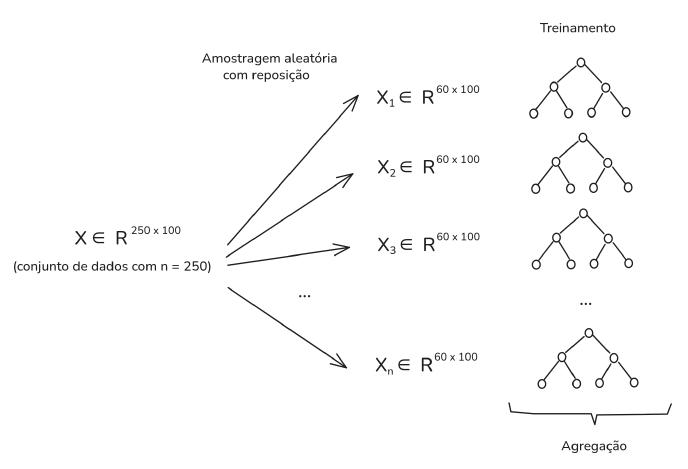
\includegraphics[scale=0.95]{pngs/RF_img.png}
\caption{Esquema simplificado do funcionamento de \DIFdelbeginFL \DIFdelFL{uma Floresta Aleatória}\DIFdelendFL \DIFaddbeginFL \DIFaddFL{um Random Forest}\DIFaddendFL .}
\label{fig:random_forest}
\end{center}
\end{figure}

\begin{figure}[htbp]
\begin{center}
	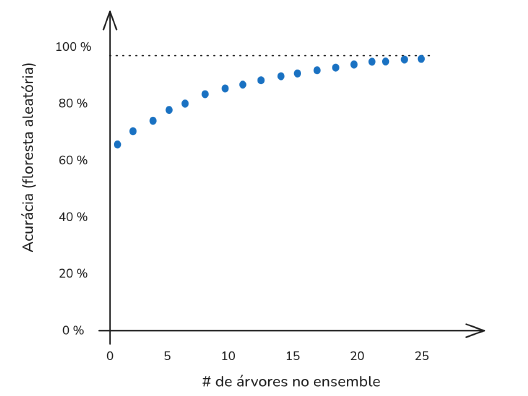
\includegraphics[scale=0.85]{pngs/manual_2.png}
\caption{Exemplo ilustrativo: 25 árvores com acurácia individual em torno de 65\% podem resultar em uma floresta com acurácia de aproximadamente 94\%.}
\label{fig:ensemble_acuracia}
\end{center}
\end{figure}

\subsection{XGBoost (\DIFdelbegin \DIFdel{eXtreme Gradient Boosting}\DIFdelend \DIFaddbegin \texorpdfstring{\textit{eXtreme Gradient Boosting}}{eXtreme Gradient Boosting}\DIFaddend )}

O \textbf{\DIFdelbegin \DIFdel{boosting}\DIFdelend \DIFaddbegin \textit{\DIFadd{boosting}}\DIFaddend } é uma família de métodos em que os modelos são treinados \textbf{um após o outro}: cada novo modelo (por exemplo, uma árvore) é ajustado para corrigir os erros do modelo anterior, de modo que a combinação de todos forme um preditor forte a partir de vários preditores \DIFdelbegin \DIFdel{"fracos" }\DIFdelend \DIFaddbegin \DIFadd{``fracos'' }\DIFaddend \citep{geron2019maos, Levada2026}. O \textbf{\DIFdelbegin \DIFdel{gradient boosting}\DIFdelend \DIFaddbegin \textit{\DIFadd{gradient boosting}}\DIFaddend } utiliza um modelo aditivo: na iteração \(m\),
\begin{equation}
\DIFdelbegin \DIFdel{F}\DIFdelend \DIFaddbegin \hat{f}\DIFaddend _m(\vec{x}) = \DIFdelbegin \DIFdel{F}\DIFdelend \DIFaddbegin \hat{f}\DIFaddend _{m-1}(\vec{x}) + \eta \, h_m(\vec{x}),
\end{equation}
onde \(h_m\) é um novo aprendiz fraco (por exemplo, uma árvore rasa) ajustado ao \textbf{gradiente negativo} da função de perda em relação à predição atual \DIFdelbegin \DIFdel{\(F_{m-1}\) }\DIFdelend \DIFaddbegin \DIFadd{\(\hat{f}_{m-1}\) }\DIFaddend --- ou seja, aos \DIFdelbegin \DIFdel{"}\DIFdelend \DIFaddbegin \DIFadd{``}\DIFaddend resíduos\DIFdelbegin \DIFdel{" }\DIFdelend \DIFaddbegin \DIFadd{'' }\DIFaddend no espaço da perda \citep{geron2019maos}. A taxa de aprendizado \(\eta\) controla a contribuição de cada árvore (encolhimento, \textit{shrinkage}), reduzindo o risco de \DIFdelbegin \DIFdel{overfitting}\DIFdelend \DIFaddbegin \textit{\DIFadd{overfitting}}\DIFaddend . O XGBoost (\textit{eXtreme Gradient Boosting}) \DIFaddbegin \DIFadd{\mbox{%DIFAUXCMD
\citep{Chen2016} }\hskip0pt%DIFAUXCMD
}\DIFaddend aprimora esse esquema \DIFdelbegin \DIFdel{ao adicionar termos de regularização explícitos na }\DIFdelend \DIFaddbegin \DIFadd{de duas maneiras. Primeiro, adiciona à }\DIFaddend função de custo \DIFdelbegin \DIFdel{(penalizando }\DIFdelend \DIFaddbegin \DIFadd{termos de regularização explícitos, que penalizam }\DIFaddend o número de folhas e os pesos das folhas\DIFdelbegin \DIFdel{) e ao utilizar }\DIFdelend \DIFaddbegin \DIFadd{. Segundo, usa }\DIFaddend uma expansão de Taylor de segunda ordem da perda para \DIFdelbegin \DIFdel{otimizar }\DIFdelend \DIFaddbegin \DIFadd{calcular }\DIFaddend a atualização de cada árvore\DIFdelbegin \DIFdel{, o que resulta em }\DIFdelend \DIFaddbegin \DIFadd{. O resultado é uma }\DIFaddend implementação eficiente e \DIFaddbegin \DIFadd{de }\DIFaddend alto desempenho \citep{geron2019maos}.

O XGBoost tornou-se muito popular em competições \DIFdelbegin \DIFdel{e }\DIFdelend \DIFaddbegin \DIFadd{de ciência de dados (como as da plataforma Kaggle) e em }\DIFaddend aplicações práticas\DIFaddbegin \DIFadd{, }\DIFaddend por sua precisão e velocidade. Em contraste com o Random Forest (que treina árvores em paralelo), o \DIFdelbegin \DIFdel{boosting }\DIFdelend \DIFaddbegin \textit{\DIFadd{boosting}} \DIFaddend é inerentemente sequencial, o que pode limitar o paralelismo em certas fases, mas o ganho de desempenho preditivo costuma compensar.
\DIFdelbegin \DIFdel{Na }\textit{\DIFdel{pipeline}} %DIFAUXCMD
\DIFdel{desta dissertação, o XGBoost é um dos quatro classificadores treinados e avaliados (Regressão Logística, Random Forest, XGBoost, CatBoost) (Capítulo 4).
}\DIFdelend 

\subsection{CatBoost}

CatBoost (\textit{Categorical Boosting}) é um algoritmo de \textit{gradient boosting} baseado em árvores, desenvolvido pela Yandex, \DIFaddbegin \DIFadd{empresa russa de tecnologia conhecida por seu mecanismo de busca \mbox{%DIFAUXCMD
\citep{Prokhorenkova2018}}\hskip0pt%DIFAUXCMD
, }\DIFaddend que incorpora inovações voltadas à robustez e à eficiência do treinamento.

Assim como o XGBoost, o CatBoost constrói árvores sequencialmente, minimizando uma função de perda por gradiente. Entretanto, \DIFaddbegin \DIFadd{sua arquitetura }\DIFaddend difere em dois aspectos \DIFdelbegin \DIFdel{arquiteturais }\DIFdelend relevantes:

\begin{itemize}
	\item \textbf{\textit{Ordered Boosting}:} para calcular os resíduos de cada exemplo, o CatBoost utiliza apenas os modelos treinados com exemplos anteriores a ele (em uma permutação aleatória do conjunto), combatendo o \textit{target leakage} (vazamento de rótulo) --- situação em que a predição de um exemplo é influenciada pelo próprio rótulo durante o treinamento. Esse procedimento reduz o viés otimista na estimativa dos resíduos, especialmente em conjuntos pequenos ou moderados.

	\item \textbf{\textit{Oblivious Decision Trees}:} cada nível da árvore aplica a \textbf{mesma condição de divisão} a todos os nós daquele nível. Essa restrição produz árvores simétricas (ou \DIFdelbegin \DIFdel{"oblivious"}\DIFdelend \DIFaddbegin \textit{\DIFadd{oblivious}}\DIFaddend ), que são mais rápidas de avaliar e atuam como regularização estrutural, reduzindo o risco de \textit{overfitting}.
\end{itemize}

O CatBoost também possui tratamento nativo de variáveis categóricas --- codificando-as internamente sem necessidade de \textit{one-hot encoding} \DIFaddbegin \DIFadd{(codificação que substitui uma variável categórica com $c$ valores possíveis por $c$ colunas binárias, uma por categoria) }\DIFaddend --- e opções para lidar com desbalanceamento de classes, como o parâmetro \DIFdelbegin \textit{\DIFdel{auto\_class\_weights='Balanced'}}%DIFAUXCMD
\DIFdelend \DIFaddbegin \texttt{\DIFadd{auto\_class\_weights='Balanced'}}\DIFaddend , que ajusta automaticamente os pesos das classes de forma inversamente proporcional à sua frequência. \DIFaddbegin \DIFadd{Neste trabalho, todas as }\textit{\DIFadd{features}} \DIFadd{são numéricas, de modo que o tratamento de variáveis categóricas não é utilizado.
}\DIFaddend 

A métrica de importância de variáveis padrão do CatBoost é o \textbf{\textit{PredictionValuesChange}}: para cada \textit{feature}, mede-se a mudança média nas predições do modelo ao longo de todos os \textit{splits} que a utilizam. Os valores são normalizados para que a soma seja igual a~100. Neste trabalho, CatBoost é utilizado junto com Regressão Logística, Random Forest e XGBoost para comparação de desempenho e robustez na classificação de curvas de luz (Capítulo~4).

% -----------------------------------------------------------------------------
\section{Agrupamento não supervisionado: K-means}
\label{sec:kmeans}

O \textbf{K-means}, proposto originalmente por \citet{MacQueen1967}, é um algoritmo de \textbf{agrupamento} (\DIFdelbegin \DIFdel{clustering}\DIFdelend \DIFaddbegin \textit{\DIFadd{clustering}}\DIFaddend ) não supervisionado: não usa rótulos; apenas particiona os dados em \DIFdelbegin \DIFdel{\(k\) }\DIFdelend \DIFaddbegin \DIFadd{\(K\) }\DIFaddend grupos de modo a minimizar a soma dos quadrados das distâncias de cada ponto ao \DIFdelbegin \DIFdel{centróide }\DIFdelend \DIFaddbegin \DIFadd{centroide }\DIFaddend do seu grupo \citep{geron2019maos, Levada2026}. A função objetivo, conhecida como \textit{Within-Cluster Sum of Squares} (WCSS) ou inércia, é
\begin{equation}
J = \sum_{i=1}\DIFdelbegin \DIFdel{^{k} }\DIFdelend \DIFaddbegin \DIFadd{^{K} }\DIFaddend \sum_{\vec{x} \in S_i} \|\vec{x} - \vec{\mu}_i\|^2,
\end{equation}
onde \(S_i\) é o conjunto de pontos atribuídos ao \DIFdelbegin \DIFdel{cluster }\DIFdelend \DIFaddbegin \textit{\DIFadd{cluster}} \DIFaddend \(i\) e \(\vec{\mu}_i\) é o \DIFdelbegin \DIFdel{centróide desse cluster}\DIFdelend \DIFaddbegin \DIFadd{centroide desse }\textit{\DIFadd{cluster}}\DIFaddend . O algoritmo alterna dois passos: (1) \textbf{atribuição} --- cada ponto é atribuído ao \DIFdelbegin \DIFdel{centróide }\DIFdelend \DIFaddbegin \DIFadd{centroide }\DIFaddend mais próximo; (2) \textbf{atualização} --- cada \DIFdelbegin \DIFdel{centróide }\DIFdelend \DIFaddbegin \DIFadd{centroide }\DIFaddend é recalculado como a média aritmética dos pontos a ele atribuídos. O custo \(J\) não aumenta a cada iteração, de modo que o processo converge para um mínimo local \citep{geron2019maos, Levada2026}. Em aplicações em que \DIFdelbegin \DIFdel{\(k\) }\DIFdelend \DIFaddbegin \DIFadd{\(K\) }\DIFaddend não é fixo, a inércia (WCSS) é frequentemente usada no \textbf{método do cotovelo} (gráfico de WCSS em função de \DIFdelbegin \DIFdel{\(k\)}\DIFdelend \DIFaddbegin \DIFadd{\(K\)}\DIFaddend ) para sugerir o número de \DIFdelbegin \DIFdel{clusters}\DIFdelend \DIFaddbegin \textit{\DIFadd{clusters}}\DIFaddend ; índices como o de \textbf{\DIFdelbegin \DIFdel{Calinski-Harabasz}\DIFdelend \DIFaddbegin \DIFadd{Cali\'nski--Harabasz}\DIFaddend }\DIFaddbegin \footnote{\DIFadd{Índice proposto por \mbox{%DIFAUXCMD
\citet{Calinski1974}}\hskip0pt%DIFAUXCMD
: $CH(K) = \dfrac{\mathrm{tr}(B_K)/(K-1)}{\mathrm{tr}(W_K)/(n-K)}$, em que $B_K$ e $W_K$ são as matrizes de dispersão entre os grupos e dentro dos grupos, e $n$ é o número de pontos. Valores maiores indicam grupos mais compactos e mais bem separados.}} \DIFaddend medem a razão entre dispersão inter e \DIFdelbegin \DIFdel{intra-cluster}\DIFdelend \DIFaddbegin \DIFadd{intra-}\textit{\DIFadd{cluster}}\DIFaddend , indicando quão bem separados estão os grupos. Para mais detalhes sobre o funcionamento \DIFdelbegin \DIFdel{deste algoritmo, fica como recomendação o paper original : }\DIFdelend \DIFaddbegin \DIFadd{do algoritmo, recomenda-se o artigo original de }\DIFaddend \citet{MacQueen1967}.

\DIFdelbegin \DIFdel{Nesta }\DIFdelend \DIFaddbegin \DIFadd{Como mencionado na Seção~\ref{sec:fundamentos_ml}, os classificadores utilizados neste trabalho são supervisionados; o uso do K-means limita-se à etapa de extração de características numéricas das curvas de luz de ocultação. Assim, nesta }\DIFaddend dissertação, o K-means \textbf{não} é usado como classificador de curvas, e sim como ferramenta para \textbf{extrair uma característica numérica}: aplica-se K-means com \(K=2\) aos valores do fluxo (ou do fluxo suavizado) de cada curva. Como não há rótulos, o algoritmo apenas descobre dois \DIFdelbegin \DIFdel{"}\DIFdelend \DIFaddbegin \DIFadd{``}\DIFaddend níveis\DIFdelbegin \DIFdel{" }\DIFdelend \DIFaddbegin \DIFadd{'' }\DIFaddend típicos nos dados \citep{Levada2026}. Os dois \DIFdelbegin \DIFdel{centróides }\DIFdelend \DIFaddbegin \DIFadd{centroides }\DIFaddend representam, grosso modo, o nível \DIFdelbegin \DIFdel{"}\DIFdelend \DIFaddbegin \DIFadd{``}\DIFaddend fora da ocultação\DIFdelbegin \DIFdel{" }\DIFdelend \DIFaddbegin \DIFadd{'' }\DIFaddend e o nível \DIFdelbegin \DIFdel{"}\DIFdelend \DIFaddbegin \DIFadd{``}\DIFaddend dentro da ocultação\DIFdelbegin \DIFdel{". A }\DIFdelend \DIFaddbegin \DIFadd{''. A }\DIFaddend \textbf{distância entre os \DIFdelbegin \DIFdel{centróides}\DIFdelend \DIFaddbegin \DIFadd{centroides}\DIFaddend } é então usada como mais uma entrada (\DIFdelbegin \DIFdel{feature}\DIFdelend \DIFaddbegin \textit{\DIFadd{feature}}\DIFaddend ) para o classificador: curvas com ocultação bem definida tendem a ter distância maior; curvas apenas ruidosas tendem a ter distância menor. \DIFdelbegin \DIFdel{O detalhe está }\DIFdelend \DIFaddbegin \DIFadd{Os detalhes estão }\DIFaddend no Capítulo\DIFaddbegin \DIFadd{~}\DIFaddend 4. No uso aqui, \DIFdelbegin \DIFdel{\(k=2\) }\DIFdelend \DIFaddbegin \DIFadd{\(K=2\) }\DIFaddend e a variável é unidimensional (fluxo), o que simplifica a interpretação.

% -----------------------------------------------------------------------------
\section{Algoritmos de otimização no treinamento}
\label{sec:otimizacao}

Em um projeto de ML supervisionado, a etapa de \textbf{treinamento} corresponde, como explicado anteriormente, a ajustar os parâmetros do modelo de modo a minimizar uma função de custo (ou perda) nos dados. Nas seções anteriores foram apresentados os modelos e suas funções de custo; aqui unificamos os \textbf{algoritmos} usados para obter o minimizador. A minimização pode ser feita por \textbf{solução analítica\DIFdelbegin \DIFdel{fechada}\DIFdelend }, quando existe fórmula explícita (como na regressão linear, Seção~\ref{sec:reglin_didatica}), ou por \textbf{algoritmos iterativos}, quando não há \DIFdelbegin \DIFdel{forma fechada}\DIFdelend \DIFaddbegin \DIFadd{solução analítica}\DIFaddend . Os três esquemas mais recorrentes são resumidos a seguir; a Tabela~\ref{tab:otimizacao} indica em que contexto cada um aparece.

\textbf{1. Mínimos quadrados (solução \DIFdelbegin \DIFdel{fechada}\DIFdelend \DIFaddbegin \DIFadd{analítica}\DIFaddend ).} Conforme visto na regressão linear (Seção~\ref{sec:reglin_didatica}), modelos lineares com custo quadrático possuem minimizador analítico dado pela equação normal \DIFdelbegin \DIFdel{\(\vec{\theta}^* = (X^\top X)^{-1} X^\top \vec{y}\)}\DIFdelend \DIFaddbegin \DIFadd{\(\vec{\theta}^* = (\mathbf{X}^\top \mathbf{X})^{-1} \mathbf{X}^\top \vec{y}\)}\DIFaddend . Na Regressão Logística e em modelos não lineares, recorre-se a métodos iterativos.

\textbf{2. Gradiente descendente (método de primeira ordem).} O \textbf{gradiente} da função de custo indica a direção de maior crescimento do custo; para minimizar, atualiza-se os parâmetros na \textbf{direção oposta}, com passo controlado pela taxa de aprendizado \(\eta\):
\[
\vec{\theta}_{t+1} = \vec{\theta}_t - \eta \, \nabla_{\vec{\theta}} J(\vec{\theta}_t).
\]
As variantes principais distinguem-se pela quantidade de dados usada em cada atualização \citep{geron2019maos}: \textbf{\DIFdelbegin \DIFdel{Batch }\DIFdelend \DIFaddbegin \textit{\DIFadd{Batch}} \DIFaddend GD} utiliza todo o conjunto de treino (preciso, mas lento em grandes volumes); \textbf{\DIFdelbegin \DIFdel{Stochastic }\DIFdelend \DIFaddbegin \textit{\DIFadd{Stochastic}} \DIFaddend GD} (SGD) utiliza uma única instância aleatória por passo (rápido e capaz de escapar de mínimos locais, mas com trajetória errática); \textbf{\DIFdelbegin \DIFdel{Mini-batch }\DIFdelend \DIFaddbegin \textit{\DIFadd{Mini-batch}} \DIFaddend GD} processa pequenos subconjuntos aleatórios, equilibrando estabilidade e eficiência. A convergência depende crucialmente de \(\eta\): se muito alta, o algoritmo pode divergir; se muito baixa, o treinamento torna-se excessivamente lento. \DIFdelbegin \DIFdel{Como vimos na Seção~\ref{sec:modelos_classificacao}, a }\DIFdelend \DIFaddbegin \DIFadd{A }\DIFaddend Regressão Logística \DIFdelbegin \DIFdel{é }\DIFdelend \DIFaddbegin \DIFadd{pode ser }\DIFaddend ajustada por gradiente descendente \DIFaddbegin \DIFadd{(Seção~\ref{sec:modelos_classificacao}), embora a implementação usada neste trabalho empregue o L-BFGS}\DIFaddend ; o mesmo esquema é usado em redes neurais e no \DIFdelbegin \DIFdel{gradient boosting }\DIFdelend \DIFaddbegin \textit{\DIFadd{gradient boosting}} \DIFaddend (cada árvore é ajustada ao gradiente da perda).

\textbf{3. Métodos de segunda ordem (Newton e variantes).} O \textbf{método de Newton} utiliza o gradiente e a \textbf{Hessiana}\DIFaddbegin \footnote{\DIFadd{Matriz das derivadas parciais de segunda ordem da função de custo, $H_{ij} = \partial^2 J / \partial\theta_i\,\partial\theta_j$, que descreve a curvatura local de $J$ \mbox{%DIFAUXCMD
\citep{Nocedal2006}}\hskip0pt%DIFAUXCMD
.}} \DIFaddend da função de custo:
\[
\vec{\theta}_{t+1} = \vec{\theta}_t - H^{-1}(\vec{\theta}_t) \, \nabla_{\vec{\theta}} J(\vec{\theta}_t).
\]
Isso permite passos mais informados e convergência mais rápida perto do mínimo, às custas de calcular e inverter \(H\) a cada iteração (custo \(O(p^3)\) por passo). Variantes \textbf{quasi-Newton}\DIFdelbegin \DIFdel{(como BFGS) }\DIFdelend \DIFaddbegin \DIFadd{, como o BFGS}\footnote{\DIFadd{Sigla de Broyden--Fletcher--Goldfarb--Shanno: o método atualiza, a cada iteração, uma aproximação de $H^{-1}$ usando apenas as variações sucessivas dos parâmetros e do gradiente \mbox{%DIFAUXCMD
\citep[cap.~6]{Nocedal2006}}\hskip0pt%DIFAUXCMD
. Sua versão de memória limitada (L-BFGS) é o }\textit{\DIFadd{solver}} \DIFadd{padrão da Regressão Logística do }\textit{\DIFadd{scikit-learn}}\DIFadd{, usado neste trabalho.}}\DIFadd{, }\DIFaddend aproximam a Hessiana sem calculá-la explicitamente. O XGBoost utiliza uma \textbf{expansão de Taylor de segunda ordem} da perda para determinar a atualização ótima de cada árvore no \DIFdelbegin \DIFdel{gradient boosting }\DIFdelend \DIFaddbegin \textit{\DIFadd{gradient boosting}} \DIFaddend \citep{geron2019maos}.

\begin{table}[htbp]
\centering
\small
\caption{Algoritmos de otimização e seu papel na etapa de treinamento em projetos de ML.}
\label{tab:otimizacao}
\DIFdelbeginFL %DIFDELCMD < \begin{tabular}{@{}p{2.2cm}p{4.1cm}p{5.2cm}@{}}
%DIFDELCMD < \hline
%DIFDELCMD < \textbf{Família} & \textbf{Exemplo} & \textbf{Onde aparece} \\
%DIFDELCMD < \hline
%DIFDELCMD < Solução fechada & Mínimos quadrados (equação normal) & Regressão linear (Seção~\ref{sec:reglin_didatica}) \\
%DIFDELCMD < \hline
%DIFDELCMD < Primeira ordem (iterativo) & Gradiente descendente (Batch, SGD, Mini-batch) & Regressão Logística, redes neurais, gradient boosting \\
%DIFDELCMD < \hline
%DIFDELCMD < Segunda ordem (iterativo) & Newton, quasi-Newton (BFGS), Taylor & XGBoost (Taylor da perda); otimização convexa em geral \\
%DIFDELCMD < \hline
%DIFDELCMD < \end{tabular}
%DIFDELCMD < %%%
\DIFdelendFL \DIFaddbeginFL \begin{tabular}{@{}p{3.0cm}p{4.8cm}p{6.2cm}@{}}
\hline
\textbf{Família} & \textbf{Exemplo} & \textbf{Onde aparece} \\
\hline
Solução analítica & Mínimos quadrados (equação normal) & Regressão linear (Seção~\ref{sec:reglin_didatica}) \\
\hline
Primeira ordem (iterativo) & Gradiente descendente (\textit{Batch}, SGD, \textit{Mini-batch}) & Exposição didática da Regressão Logística, redes neurais, \textit{gradient boosting} \\
\hline
Segunda ordem (iterativo) & Newton, quasi-Newton (BFGS, L-BFGS), Taylor & Regressão Logística desta dissertação (L-BFGS); XGBoost (Taylor da perda); otimização convexa em geral \\
\hline
\end{tabular}
\DIFaddendFL \end{table}

\DIFdelbegin \DIFdel{Com isso, o leitor dispõe de uma referência clara sobre o significado das "contas" envolvidas no treinamento de modelos de aprendizado de máquina. Inicialmente, apresentamos um modelo simples de Regressão Linear ajustado por meio do método dos mínimos quadrados e discutimos suas limitações. Em seguida, introduzimos a Regressão Logística (Seção~\ref{sec:modelos_classificacao}) como um exemplo direto de otimização por gradiente descendente. Por fim, abordamos os ensembles de árvores, que utilizam critérios de divisão para o aprendizado; no caso do XGBoost, o processo de otimização incorpora informações de segunda ordem da função de perda, resultando em atualizações mais eficientes \mbox{%DIFAUXCMD
\citep{geron2019maos}}\hskip0pt%DIFAUXCMD
.
}%DIFDELCMD < 

%DIFDELCMD < %%%
\DIFdelend % -----------------------------------------------------------------------------
\section{Engenharia de características e validação de modelos}
\label{sec:feature_validacao}

\subsection{Engenharia de características}

A criação e a seleção de \textbf{características numéricas} (atributos) a partir dos dados brutos são fundamentais para o sucesso do ML \citep{geron2019maos}, uma vez que essas variáveis representam a informação que será efetivamente utilizada pelos algoritmos para identificar padrões e realizar previsões.

Essa etapa inclui: (i)~escolher ou construir variáveis que capturem informação útil para a tarefa (por exemplo, estatísticas da curva de luz, derivadas, comparações entre segmentos); (ii)~combinar ou transformar variáveis existentes (médias móveis, suavização, testes estatísticos entre quartis, etc.). No Capítulo 4, descreve-se em detalhe o conjunto de \DIFdelbegin \DIFdel{features }\DIFdelend \DIFaddbegin \textit{\DIFadd{features}} \DIFaddend extraídas de cada curva de luz (amplitude, desvio padrão, \DIFdelbegin \DIFdel{max drawdown}\DIFdelend \DIFaddbegin \DIFadd{queda máxima acumulada (}\textit{\DIFadd{max drawdown}}\DIFadd{)}\DIFaddend , distância entre \DIFdelbegin \DIFdel{centróides }\DIFdelend \DIFaddbegin \DIFadd{centroides }\DIFaddend do K-means no fluxo, estatísticas de derivadas, \(p\)-valores entre quartis, entre outras). Essas grandezas formam o vetor \(\vec{x}\) de entrada dos classificadores.

\subsection{Métricas de avaliação para classificação binária}
\label{sec:metricas_avaliacao}

A avaliação de um classificador binário parte da \textbf{matriz de confusão}, que contabiliza os acertos e erros do modelo em relação aos rótulos verdadeiros. Sejam \(y_i \in \{0,1\}\) os rótulos reais e \(\hat{y}_i\) as predições; definem-se quatro contagens:

\begin{itemize}
	\item \textbf{Verdadeiro Positivo (TP\DIFaddbegin \DIFadd{, do inglês }\textit{\DIFadd{True Positive}}\DIFaddend ):} $\hat{y}_i = 1$ e $y_i = 1$ (acerto na classe positiva).
	\item \textbf{Verdadeiro Negativo (TN\DIFaddbegin \DIFadd{, }\textit{\DIFadd{True Negative}}\DIFaddend ):} $\hat{y}_i = 0$ e $y_i = 0$ (acerto na classe negativa).
	\item \textbf{Falso Positivo (FP\DIFaddbegin \DIFadd{, }\textit{\DIFadd{False Positive}}\DIFaddend ):} $\hat{y}_i = 1$ e $y_i = 0$ (alarme falso).
	\item \textbf{Falso Negativo (FN\DIFaddbegin \DIFadd{, }\textit{\DIFadd{False Negative}}\DIFaddend ):} $\hat{y}_i = 0$ e $y_i = 1$ (evento perdido).
\end{itemize}

A partir dessas contagens, as métricas mais utilizadas em classificação binária são:

\textbf{Acurácia} --- fração de predições corretas sobre o total:

\begin{equation}
\text{Acurácia} = \frac{TP + TN}{TP + TN + FP + FN}.
\end{equation}

A acurácia é intuitiva, mas pode ser enganosa em conjuntos desbalanceados. 

\textbf{Exemplo numérico:} considere 100 curvas de luz, das quais 10 contêm ocultação (positivas) e 90 não (negativas). Um classificador que \textbf{sempre} prediz \DIFdelbegin \DIFdel{"negativo" }\DIFdelend \DIFaddbegin \DIFadd{``negativo'' }\DIFaddend acerta 90 das 100 curvas --- acurácia de 90\% --- mas não detecta \textit{nenhuma} ocultação ($\text{sensibilidade} = 0$). Esse paradoxo evidencia que, em cenários desbalanceados, a acurácia sozinha é insuficiente para avaliar o modelo.

\textbf{Precisão} (\textit{Precision}) --- entre os exemplos classificados como positivos, qual fração é realmente positiva:
\begin{equation}
\text{Precisão} = \frac{TP}{TP + FP}.
\end{equation}

\textbf{Sensibilidade} (\textit{Recall}, ou sensibilidade) --- entre os exemplos verdadeiramente positivos, qual fração foi corretamente detectada:
\begin{equation}
\text{Sensibilidade} = \frac{TP}{TP + FN}.
\end{equation}

\textbf{F1-score} --- média harmônica de precisão e sensibilidade, oferecendo um compromisso entre ambas:
\begin{equation}
F_1 = 2 \cdot \frac{\text{Precisão} \cdot \text{Sensibilidade}}{\text{Precisão} + \text{Sensibilidade}} = \frac{2\,TP}{2\,TP + FP + FN}.
\end{equation}

\textbf{F$_\beta$-score} --- generalização do F1-score que permite atribuir peso diferente à sensibilidade:
\begin{equation}
F_\beta = (1 + \beta^2) \cdot \frac{\text{Precisão} \cdot \text{Sensibilidade}}{\beta^2 \cdot \text{Precisão} + \text{Sensibilidade}}.
\end{equation}
Para $\beta > 1$, o $F_\beta$ penaliza mais os falsos negativos (favorecendo a sensibilidade); para $\beta < 1$, penaliza mais os falsos positivos. Em aplicações de triagem científica, como a detecção de ocultações estelares, $\beta = 2$ é uma escolha natural, pois o custo de perder um evento genuíno \DIFdelbegin \DIFdel{(FN) }\DIFdelend é maior que o de investigar um alarme falso\DIFdelbegin \DIFdel{(FP) \mbox{%DIFAUXCMD
\citep{Saito2015}}\hskip0pt%DIFAUXCMD
}\DIFdelend \DIFaddbegin \DIFadd{, isto é, o custo de um FN supera o de um FP}\DIFaddend .

\textbf{AUC-ROC} (\textit{Area Under the Receiver Operating Characteristic Curve}) --- mede a capacidade discriminativa do modelo ao longo de todos os limiares de decisão possíveis. A curva ROC plota a \textbf{taxa de verdadeiros positivos} (sensibilidade) contra a \textbf{taxa de falsos positivos} ($FP/(FP+TN)$) para cada limiar $\tau$. A área sob essa curva (AUC) varia de 0,5 (classificador aleatório) a 1,0 (classificador perfeito), como mostrado na \DIFdelbegin \DIFdel{imagem \ref{fig:roc_auc}. }\DIFdelend \DIFaddbegin \DIFadd{Figura~\ref{fig:roc_auc}: quanto mais a curva se aproxima do canto superior esquerdo, melhor a capacidade discriminativa do modelo. Um exemplo intuitivo é um teste médico: a taxa de verdadeiros positivos é a fração de doentes corretamente identificados, a taxa de falsos positivos é a fração de saudáveis apontados como doentes, e variar o limiar move o teste ao longo da curva, negociando a detecção de mais doentes contra um número maior de alarmes falsos. }\DIFaddend A AUC-ROC é útil por ser invariante ao limiar escolhido, mas pode ser otimista em conjuntos desbalanceados \citep{Saito2015}.

\begin{figure}[h!]
\begin{center}
	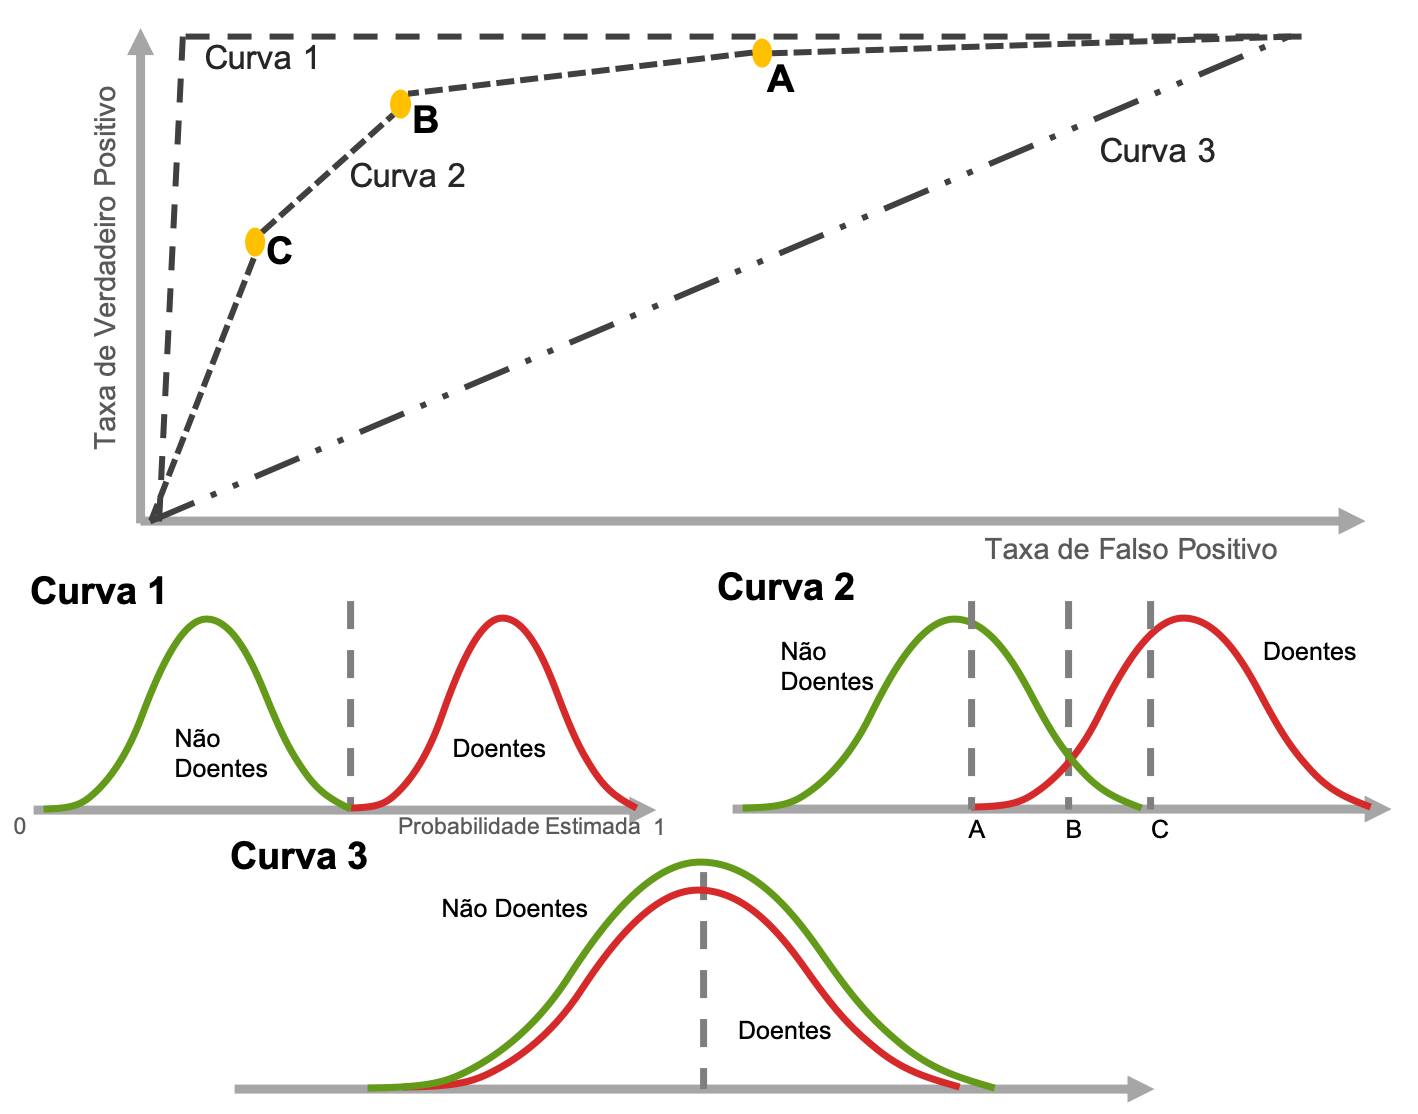
\includegraphics[width=0.75\textwidth]{pngs/roc_curvas_todas_ref_httpscienciaenegocios.comcurva-roc-e-auc-em-machine-learning.png}
\DIFdelbeginFL %DIFDELCMD < \caption{%%%
\DIFdelendFL \DIFaddbeginFL \caption[Exemplos de curvas ROC]{\DIFaddendFL Exemplos de curvas ROC para classificadores de diferentes qualidades\DIFdelbeginFL \DIFdelFL{: quanto mais a curva se aproxima do canto superior esquerdo (maior área sob a curva, AUC), melhor a capacidade discriminativa do modelo}\DIFdelendFL ; a diagonal corresponde a um classificador aleatório (AUC = 0,5). \DIFdelbeginFL \DIFdelFL{Um exemplo intuitivo é um teste médico que classifica pacientes como doentes ou saudáveis}\DIFdelendFL \DIFaddbeginFL \DIFaddFL{Fonte}\DIFaddendFL : \DIFdelbeginFL \DIFdelFL{a taxa }\DIFdelendFL \DIFaddbeginFL \DIFaddFL{adaptado }\DIFaddendFL de \DIFdelbeginFL \DIFdelFL{verdadeiros positivos mede a fração de doentes corretamente identificados, enquanto a taxa de falsos positivos mede a fração de saudáveis erroneamente apontados como doentes}\DIFdelendFL \DIFaddbeginFL \DIFaddFL{Ciência e Negócios}\DIFaddendFL . \DIFdelbeginFL \DIFdelFL{Variar o limiar de decisão move o teste ao longo da curva, negociando a detecção de mais doentes contra um número maior de alarmes falsos}\DIFdelendFL \DIFaddbeginFL \DIFaddFL{Disponível em: }\url{https://cienciaenegocios.com/curva-roc-e-auc-em-machine-learning}\DIFaddendFL . \DIFdelbeginFL \DIFdelFL{Fonte}\DIFdelendFL \DIFaddbeginFL \DIFaddFL{Acesso em}\DIFaddendFL : \DIFdelbeginFL \DIFdelFL{adaptado de }\emph{\DIFdelFL{Ciência e Negócios}}%DIFAUXCMD
%DIFDELCMD < \protect\footnotemark%%%
\DIFdelendFL \DIFaddbeginFL \DIFaddFL{6 abr}\DIFaddendFL . \DIFaddbeginFL \DIFaddFL{2026.}\DIFaddendFL }
\label{fig:roc_auc}
\end{center}
\end{figure}
\DIFdelbegin \footnotetext{\DIFdel{Disponível em: }%DIFDELCMD < \url{https://cienciaenegocios.com/curva-roc-e-auc-em-machine-learning}%%%
\DIFdel{. Acesso em: 6 abr. 2026.}}
%DIFAUXCMD
\DIFdelend 

\textbf{Curva Precisão-Sensibilidade} (\textit{Precision-Recall}) --- alternativa à curva ROC, recomendada quando a classe positiva é rara ou quando o custo dos erros é assimétrico \citep{Saito2015}. Plota a precisão contra a sensibilidade para cada limiar~$\tau$. A área sob a curva PR (AUC-PR) é mais informativa que a AUC-ROC em cenários desbalanceados, pois não é inflada por verdadeiros negativos abundantes.

Nesta dissertação, os modelos são avaliados por acurácia, precisão, sensibilidade, F1-score e AUC-ROC no conjunto de teste (Capítulo~5). Para a análise de ajuste de limiar, utilizam-se também o $F_2$-score e a curva \DIFdelbegin \DIFdel{precision-recall}\DIFdelend \DIFaddbegin \textit{\DIFadd{precision-recall}}\DIFaddend .

\subsection{\DIFdelbegin \DIFdel{Overfitting, underfitting }\DIFdelend \DIFaddbegin \texorpdfstring{\textit{Overfitting}, \textit{underfitting}}{Overfitting, underfitting} \DIFaddend e o compromisso entre viés e variância}
\label{sec:overfitting}

A identificação de \textbf{sobreajuste} (\DIFdelbegin \DIFdel{overfitting}\DIFdelend \DIFaddbegin \textit{\DIFadd{overfitting}}\DIFaddend ) e \textbf{subajuste} (\DIFdelbegin \DIFdel{underfitting}\DIFdelend \DIFaddbegin \textit{\DIFadd{underfitting}}\DIFaddend ) baseia-se na comparação do desempenho do modelo nos dados usados no treinamento versus nos dados reservados para teste ou validação \citep{geron2019maos}. Em termos intuitivos: \textbf{sobreajuste} ocorre quando o modelo \DIFdelbegin \DIFdel{"decora" }\DIFdelend \DIFaddbegin \DIFadd{``decora'' }\DIFaddend os dados de treino (incluindo o ruído) e deixa de generalizar --- o erro no treino fica muito baixo, mas o erro em dados novos permanece alto. \textbf{Subajuste} ocorre quando o modelo é simples demais e não captura o padrão verdadeiro dos dados --- tanto o erro de treino quanto o de validação ficam altos. 

O erro de generalização pode ser decomposto em \textbf{viés}, \textbf{variância} e \textbf{ruído irredutível} \citep{Deisenroth2019, Levada2026}. Formalmente, \DIFdelbegin \DIFdel{para um modelo }\DIFdelend \DIFaddbegin \DIFadd{seja $f^\star(\vec{x})$ a relação verdadeira (desconhecida) entre entrada e saída e }\DIFaddend $\hat{f}$ \DIFdelbegin \DIFdel{treinado em diferentes amostras }\DIFdelend \DIFaddbegin \DIFadd{o modelo --- a função $f$ da Seção~\ref{sec:problema_classificacao} --- estimado a partir de diferentes amostras de treino }\DIFaddend do mesmo processo gerador\DIFdelbegin \DIFdel{, }\DIFdelend \DIFaddbegin \DIFadd{; }\DIFaddend o erro quadrático médio esperado em um ponto $\vec{x}$ é:
\begin{equation}
\mathbb{E}\!\left[(y - \hat{f}(\vec{x}))^2\right] = \text{Viés}^2[\hat{f}(\vec{x})] + \text{Var}[\hat{f}(\vec{x})] + \sigma^2,
\label{eq:bias_variance}
\end{equation}
onde \DIFdelbegin \DIFdel{$\text{Viés}^2[\hat{f}] = \left(\mathbb{E}[\hat{f}(\vec{x})] - f(\vec{x})\right)^2$ }\DIFdelend \DIFaddbegin \DIFadd{$\text{Viés}^2[\hat{f}] = \left(\mathbb{E}[\hat{f}(\vec{x})] - f^\star(\vec{x})\right)^2$ }\DIFaddend mede o erro sistemático do modelo (quão longe a predição média está do valor verdadeiro), $\text{Var}[\hat{f}]$ mede a sensibilidade do modelo a flutuações nos dados de treino, e $\sigma^2$ é a variância do ruído intrínseco aos dados (irredutível por qualquer modelo). Modelos muito simples tendem a alto viés (subajuste); modelos muito flexíveis tendem a alta variância (sobreajuste). O objetivo prático é encontrar um equilíbrio que minimize o erro total.

\textbf{Diagnóstico.} O sinal mais claro de sobreajuste é um erro muito baixo no treino e um erro alto no teste ou validação (não generalizou). Esse diagnóstico é feito graficamente pelas \textbf{curvas de aprendizado} (Seção~\ref{sec:curvas_aprendizado}): o sobreajuste aparece como um \textbf{gap} entre a curva de treino e a de validação, enquanto o subajuste mantém ambas próximas e em um \textbf{platô alto} de erro.

A \textbf{validação cruzada} --- detalhada na Seção~\ref{sec:validacao_modelos} --- complementa esse diagnóstico ao fornecer uma estimativa robusta do erro de generalização (média e desvio padrão sobre várias divisões dos dados), facilitando perceber quando o modelo começou a sobreajustar \citep{geron2019maos}.

Em resumo: \textbf{sobreajuste} (\DIFdelbegin \DIFdel{overfitting}\DIFdelend \DIFaddbegin \textit{\DIFadd{overfitting}}\DIFaddend ) significa que o modelo se ajustou demais aos dados de treino (incluindo o ruído) e perde capacidade de generalizar; soluções típicas são obter mais dados, simplificar o modelo ou usar regularização (penalizar parâmetros grandes). \textbf{Subajuste} (\DIFdelbegin \DIFdel{underfitting}\DIFdelend \DIFaddbegin \textit{\DIFadd{underfitting}}\DIFaddend ) significa que o modelo é simples demais e não captura o padrão dos dados; as soluções envolvem aumentar a complexidade do modelo ou enriquecer as características de entrada. Os \textbf{hiperparâmetros} (por exemplo, força da regularização, profundidade máxima das árvores) controlam esse equilíbrio e podem ser escolhidos via validação cruzada.

A \textbf{regularização} restringe a liberdade do modelo (por exemplo, penalidade \(\ell_2\) na Regressão Logística ou limites de profundidade e número de folhas nas árvores), sendo controlada por hiperparâmetros que podem ser ajustados via validação cruzada \citep{geron2019maos}. Outras formas incluem a \textbf{parada antecipada}: interromper o treinamento quando o erro no conjunto de validação deixa de melhorar, evitando que o modelo \DIFdelbegin \DIFdel{"decore" }\DIFdelend \DIFaddbegin \DIFadd{``decore'' }\DIFaddend o ruído do treino. Nesta dissertação, o foco está na penalização \DIFdelbegin \DIFdel{de pesos em modelos lineares (Ridge/Lasso) e nos critérios de parada e poda }\DIFdelend \DIFaddbegin \DIFadd{$\ell_2$ da Regressão Logística e nos limites de profundidade e de número mínimo de amostras por nó e por folha }\DIFaddend nas árvores \DIFaddbegin \DIFadd{(não se aplica poda)}\DIFaddend . A regularização \(\ell_1\) e \(\ell_2\) é \textbf{sensível à escala} das variáveis de entrada: atributos em escalas maiores tendem a receber pesos menores pela penalização. Em geral, recomenda-se \textbf{padronizar} as variáveis (subtrair a média e dividir pelo desvio padrão) antes de aplicar Ridge ou Lasso. \DIFdelbegin %DIFDELCMD < 

%DIFDELCMD < %%%
\DIFdel{Na }\textit{\DIFdel{pipeline}} %DIFAUXCMD
\DIFdel{desta dissertação, as features não }\DIFdelend \DIFaddbegin \DIFadd{No entanto, nesta dissertação a padronização é aplicada apenas à Regressão Logística; os modelos baseados em árvores recebem as }\textit{\DIFadd{features}} \DIFadd{na escala original, pois }\DIFaddend são \DIFdelbegin \DIFdel{padronizadas antes de todos os treinos }\DIFdelend \DIFaddbegin \DIFadd{insensíveis a transformações monotônicas de cada variável }\DIFaddend (Capítulo\DIFaddbegin \DIFadd{~}\DIFaddend 4)\DIFdelbegin \DIFdel{; a justificativa é discutida naquele capítulo}\DIFdelend .

\subsection{Curvas de aprendizado}
\label{sec:curvas_aprendizado}

As \textbf{curvas de aprendizado} mostram o desempenho do modelo (acurácia ou erro) em função do tamanho do conjunto de treino (ou do número de épocas); são a ferramenta gráfica que torna visível o equilíbrio viés--variância discutido acima e auxiliam na decisão de coletar mais dados ou alterar a complexidade do modelo.

A Figura~\ref{fig:learning_curves} ilustra o conceito com curvas de aprendizado \DIFdelbegin \DIFdel{reais de três classificadores (XGBoost, Random Forest e Árvore de Decisão)em uma tarefa }\DIFdelend de \DIFaddbegin \DIFadd{seis classificadores --- (A)~XGBoost, (B)~Random Forest, (C)~árvore de decisão, (D)~}\textit{\DIFadd{Extra Trees}}\DIFadd{, (E)~}\textit{\DIFadd{Naive Bayes}} \DIFadd{gaussiano e (F)~Regressão Logística --- aplicados a um problema de }\DIFaddend classificação \DIFaddbegin \DIFadd{em medicina \mbox{%DIFAUXCMD
\citep{Zhong2023}}\hskip0pt%DIFAUXCMD
}\DIFaddend . Em cada painel, a curva superior é o desempenho no \textbf{treino} e a inferior o desempenho em \textbf{validação cruzada}, ambos em função do número de amostras de treino. Dois padrões didáticos aparecem: (i)~a curva de validação \textbf{sobe} à medida que mais dados ficam disponíveis e tende a um \textbf{platô}, ponto a partir do qual coletar mais exemplos pouco acrescenta; (ii)~o \textbf{intervalo} (\textit{gap}) entre a curva de treino (quase perfeita) e a de validação mede o \textbf{sobreajuste} --- quanto maior o vão, mais o modelo decorou o treino em vez de generalizar. Um modelo bem ajustado é aquele cujas duas curvas convergem para um patamar alto com vão pequeno\DIFdelbegin \DIFdel{.
}\DIFdelend \DIFaddbegin \DIFadd{; na figura, é o caso do XGBoost (painel A), cujas curvas convergem para $\approx 0{,}96$. Os painéis E e F ilustram o subajuste: as curvas se encontram, mas num patamar baixo ($\approx 0{,}67$ e $\approx 0{,}74$). Com poucos exemplos de treino, todos os modelos mostram o vão largo típico do sobreajuste.
}\DIFaddend 

\begin{figure}[h!]
\begin{center}
	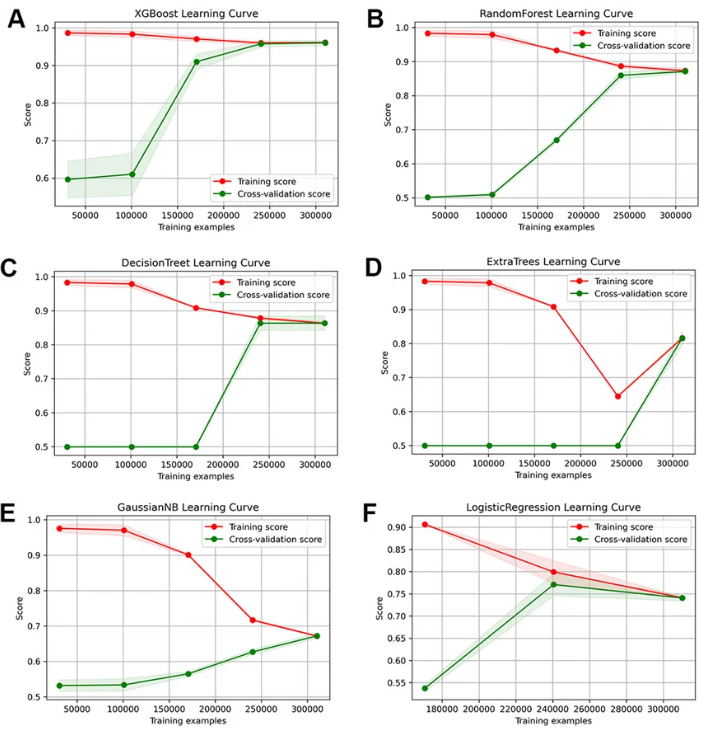
\includegraphics[width=0.8\textwidth]{pngs/Learning-curves-of-models-with-training-data-A-XGBoost-B-Random-Forest-C.png}
\DIFdelbeginFL %DIFDELCMD < \caption{%%%
\DIFdelendFL \DIFaddbeginFL \caption[Exemplo de curvas de aprendizado]{\DIFaddendFL Exemplo de curvas de aprendizado (dados genéricos, não referentes a curvas de luz de ocultação) para \DIFdelbeginFL \DIFdelFL{três }\DIFdelendFL \DIFaddbeginFL \DIFaddFL{seis }\DIFaddendFL classificadores: (A)~XGBoost, (B)~Random Forest\DIFdelbeginFL \DIFdelFL{e }\DIFdelendFL \DIFaddbeginFL \DIFaddFL{, }\DIFaddendFL (C)~\DIFdelbeginFL \DIFdelFL{Árvore }\DIFdelendFL \DIFaddbeginFL \DIFaddFL{árvore }\DIFaddendFL de \DIFdelbeginFL \DIFdelFL{Decisão}\DIFdelendFL \DIFaddbeginFL \DIFaddFL{decisão, (D)~}\textit{\DIFaddFL{Extra Trees}}\DIFaddFL{, (E)~}\textit{\DIFaddFL{Naive Bayes}} \DIFaddFL{gaussiano e (F)~Regressão Logística}\DIFaddendFL . Em cada painel, compara-se o desempenho no conjunto de treino com o obtido em validação cruzada, em função do número de amostras de treino\DIFdelbeginFL \DIFdelFL{; o vão entre as duas curvas indica o grau de sobreajuste, e o platô da curva de validação indica a partir de quando mais dados deixam de melhorar o modelo}\DIFdelendFL . Fonte: \DIFdelbeginFL \DIFdelFL{adaptado de }\emph{\DIFdelFL{ResearchGate}}%DIFAUXCMD
%DIFDELCMD < \protect\footnotemark%%%
\DIFdelendFL \DIFaddbeginFL \DIFaddFL{\mbox{%DIFAUXCMD
\citet{Zhong2023}}\hskip0pt%DIFAUXCMD
}\DIFaddendFL .}
\label{fig:learning_curves}
\end{center}
\end{figure}
\DIFdelbegin \footnotetext{\DIFdel{Disponível em: }%DIFDELCMD < \url{https://www.researchgate.net/figure/Learning-curves-of-models-with-training-data-A-XGBoost-B-Random-Forest-C_fig2_374986649}%%%
\DIFdel{. Acesso em: 6 abr. 2026.}}
%DIFAUXCMD
\DIFdelend 

\subsection{Validação de modelos}
\label{sec:validacao_modelos}

Para estimar o desempenho em dados não vistos e evitar otimismo, é essencial separar os dados usados no treino daqueles usados na avaliação \citep{geron2019maos}. \DIFdelbegin \DIFdel{Imagine que treinamos o modelo usando }\DIFdelend \DIFaddbegin \DIFadd{Suponha que o modelo seja treinado com }\DIFaddend todas as curvas de luz disponíveis e depois \DIFdelbegin \DIFdel{o avaliamos }\DIFdelend \DIFaddbegin \DIFadd{avaliado }\DIFaddend nessas mesmas curvas. O resultado seria enganosamente bom. Para estimar honestamente o desempenho, é preciso reservar dados que o modelo nunca viu. A \textbf{validação cruzada} sistematiza esse processo: em vez de uma única divisão treino/teste (\DIFdelbegin \DIFdel{que pode ser sortuda ou azarada), roda-se o experimento $k$ }\DIFdelend \DIFaddbegin \DIFadd{cujo resultado pode ser favorável ou desfavorável por acaso), repete-se o experimento $q$ }\DIFaddend vezes, cada vez deixando uma fatia diferente de fora \DIFaddbegin \DIFadd{(Figura~\ref{fig:kfold})}\DIFaddend . A média dos \DIFdelbegin \DIFdel{$k$ }\DIFdelend \DIFaddbegin \DIFadd{$q$ }\DIFaddend resultados é uma estimativa muito mais robusta do erro de generalização.

\begin{figure}[htbp]
\begin{center}
	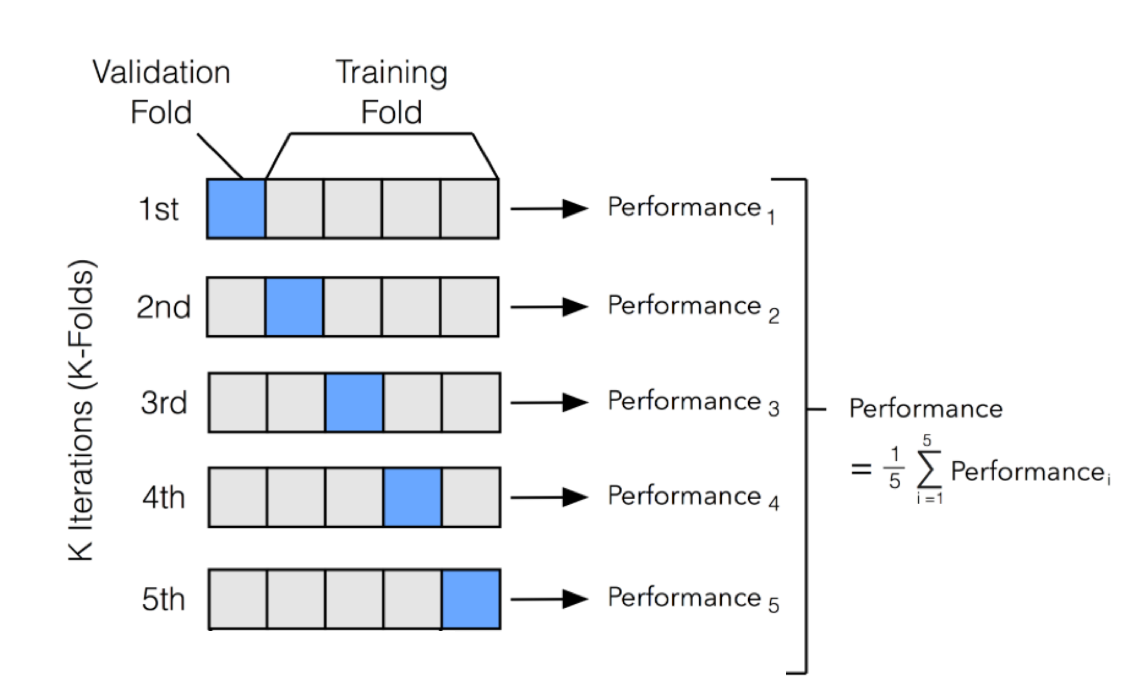
\includegraphics[width=0.75\textwidth]{pngs/kfold.png}
\DIFdelbeginFL %DIFDELCMD < \caption{%%%
\DIFdelendFL \DIFaddbeginFL \caption[Esquema da validação cruzada com $q = 5$ dobras]{\DIFaddendFL Esquema da validação cruzada com \DIFdelbeginFL \DIFdelFL{$k=5$}\DIFdelendFL \DIFaddbeginFL \DIFaddFL{$q = 5$ dobras}\DIFaddendFL : em cada rodada, uma fatia diferente (em destaque) é usada como conjunto de validação, e as demais como treino. Fonte: adaptado de Nishad~(2023)\DIFdelbeginFL %DIFDELCMD < \protect\footnotemark%%%
\DIFdelendFL . \DIFaddbeginFL \DIFaddFL{Disponível em: }\url{https://medium.com/@nishad009adi/k-fold-cross-validation-with-simple-example-e023bb2e2d43}\DIFaddFL{. Acesso em: 6 abr. 2026.}\DIFaddendFL }
\label{fig:kfold}
\end{center}
\end{figure}
\DIFdelbegin \footnotetext{\DIFdel{Disponível em: 
}%DIFDELCMD < 

%DIFDELCMD < \url{https://medium.com/@nishad009adi/k-fold-cross-validation-with-simple-example-e023bb2e2d43}%%%
\DIFdel{. Acesso em: 6 abr. 2026.}}
%DIFAUXCMD
\DIFdelend 

As estratégias mais comuns são:

\begin{itemize}
	\item \textbf{Conjunto de teste:} uma fração dos dados é reservada e nunca usada no treino; o desempenho nesse conjunto fornece uma estimativa do erro de generalização.
	\item \textbf{Validação cruzada \DIFdelbegin \DIFdel{(k-fold):}\DIFdelend \DIFaddbegin \DIFadd{em $q$ dobras}\DIFaddend } \DIFaddbegin \DIFadd{(em inglês, }\textit{\DIFadd{k-fold cross-validation}}\DIFadd{): }\DIFaddend os dados são divididos em \DIFdelbegin \DIFdel{\(k\) }\DIFdelend \DIFaddbegin \DIFadd{\(q\) }\DIFaddend partes (dobras); em cada rodada, \DIFdelbegin \DIFdel{\(k-1\) }\DIFdelend \DIFaddbegin \DIFadd{\(q-1\) }\DIFaddend dobras são usadas para treino e uma para validação; a métrica final é a média sobre as \DIFdelbegin \DIFdel{\(k\) }\DIFdelend \DIFaddbegin \DIFadd{\(q\) }\DIFaddend rodadas. Isso dá uma estimativa mais estável do desempenho e é útil para comparar modelos ou escolher hiperparâmetros (parâmetros do algoritmo que não são ajustados pelo treinamento, como a força da regularização).
	\item \textbf{Validação cruzada estratificada:} quando as classes são desbalanceadas (por exemplo, poucas curvas com ocultação e muitas sem), a divisão aleatória simples pode produzir dobras em que uma das classes está sub ou sobrerrepresentada. A validação \textbf{estratificada} preserva a proporção de cada classe em cada dobra, tornando a estimativa mais confiável \citep{geron2019maos}. Na detecção de ocultações, o uso de divisão estratificada é recomendado.
	\item \textbf{Busca em grade:} para escolher hiperparâmetros, avalia-se um conjunto de combinações (a \DIFdelbegin \DIFdel{"grade"}\DIFdelend \DIFaddbegin \DIFadd{``grade''}\DIFaddend ) e escolhe-se a que maximiza a métrica de validação.
\end{itemize}

Na \textit{pipeline} desta dissertação (\DIFdelbegin \DIFdel{Capítulo }\DIFdelend \DIFaddbegin \DIFadd{Capítulos~}\DIFaddend 4 \DIFdelbegin \DIFdel{), a divisão treino/}\DIFdelend \DIFaddbegin \DIFadd{e~5), adota-se o seguinte protocolo: (i)~um conjunto de }\DIFaddend teste é \DIFdelbegin \DIFdel{feita de forma estratificada (mantendo a proporção de positivas e negativas em cada parte) ou por seleção manual de curvas para o }\DIFdelend \DIFaddbegin \DIFadd{reservado antes de qualquer escolha de modelagem, com divisão estratificada e }\textbf{\DIFadd{agrupada por evento}} \DIFadd{(todas as curvas de um mesmo evento de ocultação --- cordas de observadores diferentes e os recortes derivados delas --- ficam do mesmo lado da divisão); (ii)~todas as escolhas (a configuração de }\textit{\DIFadd{features}} \DIFadd{e o limiar de decisão de cada modelo) são feitas por validação cruzada estratificada e agrupada no restante dos dados; (iii)~o conjunto de }\DIFaddend teste \DIFaddbegin \DIFadd{é usado uma única vez, ao final, para estimar o desempenho dos modelos escolhidos}\DIFaddend . As métricas \DIFaddbegin \DIFadd{finais }\DIFaddend (acurácia, precisão, sensibilidade, F1-score, AUC-ROC) são\DIFaddbegin \DIFadd{, portanto, }\DIFaddend calculadas no \textbf{conjunto de teste} --- dados que \DIFdelbegin \DIFdel{o modelo nunca viu durante o treinamento }\DIFdelend \DIFaddbegin \DIFadd{não foram usados no treinamento nem nas escolhas de configuração, modelo e limiar.
}

\DIFadd{Em resumo, este capítulo percorreu os procedimentos de cálculo envolvidos no treinamento de modelos de aprendizado de máquina. Inicialmente, apresentamos um modelo simples de Regressão Linear ajustado por meio do método dos mínimos quadrados e discutimos suas limitações. Em seguida, introduzimos a Regressão Logística (Seção~\ref{sec:modelos_classificacao}) como exemplo de otimização iterativa (gradiente descendente, na exposição; L-BFGS, na implementação). Depois, abordamos os }\textit{\DIFadd{ensembles}} \DIFadd{de árvores, que utilizam critérios de divisão para o aprendizado; no caso do XGBoost, o processo de otimização incorpora informações de segunda ordem da função de perda, resultando em atualizações mais eficientes \mbox{%DIFAUXCMD
\citep{geron2019maos}}\hskip0pt%DIFAUXCMD
. Por fim, esta seção reuniu as métricas de avaliação e os procedimentos de validação}\DIFaddend . Com isso, o capítulo fornece a base conceitual necessária para interpretar a metodologia e os resultados descritos \DIFdelbegin \DIFdel{no Capítulo 4.
}\DIFdelend \DIFaddbegin \DIFadd{nos Capítulos~4 e~5.
}\DIFaddend 


\chapter{Metodologia: \DIFdelbegin \DIFdel{Pipeline }\DIFdelend \DIFaddbegin \texorpdfstring{\textit{Pipeline}}{Pipeline} \DIFaddend de Detecção}

% =============================================================================
%DIF <  Capítulo 4 — Metodologia: Pré-processamento e Engenharia de Características
%DIF >  Capítulo 4 --- Metodologia: Pré-processamento e Engenharia de Características
% =============================================================================

Este capítulo descreve a metodologia adotada para desenvolver o \textbf{fluxo de trabalho em etapas} (\textit{pipeline}) de detecção automatizada de ocultações estelares em curvas de luz. A exposição está organizada em etapas sucessivas: desde a aquisição e o armazenamento dos dados até o \textbf{treinamento} (ajuste dos parâmetros dos classificadores) e a \textbf{avaliação} (medida do desempenho em dados não usados no ajuste). 

Os objetivos deste capítulo são: (1) descrever a arquitetura completa da \textit{pipeline}, da coleta dos dados ao modelo treinado; (2) detalhar o pré-processamento das curvas de luz, incluindo fontes de dados, armazenamento em banco relacional, normalização e critérios de classificação; (3) explicar a construção do conjunto de dados utilizado no treinamento, incluindo o recorte de segmentos negativos a partir de curvas positivas e a incorporação de curvas \DIFdelbegin \DIFdel{sintéticas}\DIFdelend \DIFaddbegin \DIFadd{simuladas}\DIFaddend ; (4) formalizar a engenharia de características (\textit{feature engineering}) aplicada às curvas; e (5) especificar o protocolo de treinamento e avaliação dos classificadores, com as métricas e a divisão treino/teste adotadas. Ao final, o leitor terá uma visão clara de como os dados brutos são transformados em um conjunto de atributos e como os modelos são treinados e avaliados, preparando o terreno para a discussão dos resultados no Capítulo 5.

% -----------------------------------------------------------------------------
\section{Visão geral da \DIFdelbegin \DIFdel{pipeline}\DIFdelend \DIFaddbegin \texorpdfstring{\textit{pipeline}}{pipeline}\DIFaddend }
\label{sec:visao_geral}

A metodologia está organizada em uma \textit{pipeline} em etapas, na qual a saída de um bloco alimenta o seguinte. Essa estrutura facilita a manutenção, a reprodução e a extensão do trabalho. A Figura~\ref{fig:diagrama_pipeline} ilustra o fluxo desde as fontes de dados até os modelos treinados.

\textbf{Etapa 1 \DIFdelbegin \DIFdel{— }\DIFdelend \DIFaddbegin \DIFadd{--- }\DIFaddend Aquisição e armazenamento:} curvas de luz são obtidas a partir de portais externos (VizieR, banco do Grupo do Rio) e inseridas em um banco de dados relacional SQLite, com duas tabelas principais: \texttt{observations} (metadados da observação) e \texttt{light\_curves} (pontos tempo--fluxo).

\textbf{Etapa 2 \DIFdelbegin \DIFdel{— }\DIFdelend \DIFaddbegin \DIFadd{--- }\DIFaddend Acesso e normalização:} um módulo de acesso aos dados consulta o banco, filtra curvas por objeto, data e tipo (positiva ou negativa), aplica normalização do fluxo \DIFdelbegin \DIFdel{(baseline estimado por quartis) }\DIFdelend \DIFaddbegin \DIFadd{pela linha de base (}\textit{\DIFadd{baseline}}\DIFadd{, o nível de fluxo fora da ocultação), estimada por quartis, }\DIFaddend e remove \textit{outliers} quando necessário.

\textbf{Etapa 3 \DIFdelbegin \DIFdel{— }\DIFdelend \DIFaddbegin \DIFadd{--- }\DIFaddend Construção do conjunto de dados:} as curvas disponíveis são reunidas; segmentos sem ocultação são recortados de curvas positivas (com revisão manual) para ampliar a classe negativa; curvas \DIFdelbegin \DIFdel{sintéticas negativas }\DIFdelend \DIFaddbegin \DIFadd{negativas simuladas }\DIFaddend são incorporadas. Em seguida, cada curva é convertida em um vetor de características (lista de números que a descrevem), formando uma tabela em que cada linha é uma curva e cada coluna é uma dessas grandezas.

\textbf{Etapa 4 \DIFdelbegin \DIFdel{— }\DIFdelend \DIFaddbegin \DIFadd{--- }\DIFaddend Extração de características:} para cada curva (série tempo--fluxo), \DIFdelbegin \DIFdel{são calculadas }\DIFdelend \DIFaddbegin \DIFadd{calculam-se grandezas numéricas que a resumem --- }\DIFaddend estatísticas \DIFaddbegin \DIFadd{do fluxo, da série suavizada e de suas derivadas numéricas, }\DIFaddend e \DIFdelbegin \DIFdel{medidas derivadas (suavização, derivadas, }\DIFdelend comparações \DIFdelbegin \DIFdel{entre quartis, etc.), }\DIFdelend \DIFaddbegin \DIFadd{estatísticas entre quartis temporais ---, }\DIFaddend gerando a tabela de vetores da etapa 3. O Capítulo 3 já introduziu a ideia de \textit{features}; aqui detalhamos quais grandezas são extraídas.

\textbf{Etapa 5 \DIFdelbegin \DIFdel{— }\DIFdelend \DIFaddbegin \DIFadd{--- }\DIFaddend Treinamento e avaliação:} \DIFdelbegin \DIFdel{o conjunto de dados final }\DIFdelend \DIFaddbegin \DIFadd{um }\textbf{\DIFadd{conjunto de teste}} \DIFaddend é \DIFdelbegin \DIFdel{dividido em }\textbf{\DIFdel{treino}} %DIFAUXCMD
\DIFdel{(usado para ajustar os parâmetros dos classificadores)e }\textbf{\DIFdel{teste}} %DIFAUXCMD
\DIFdel{(reservado para medir o desempenho). Os quatro classificadores }\DIFdelend \DIFaddbegin \DIFadd{reservado antes de qualquer escolha de modelagem; no restante dos dados (}\textbf{\DIFadd{conjunto de desenvolvimento}}\DIFadd{), a configuração de }\textit{\DIFadd{features}} \DIFadd{e o limiar de decisão de cada modelo }\DIFaddend são \DIFdelbegin \DIFdel{treinados na parte de treino; o desempenho é avaliado na parte de }\DIFdelend \DIFaddbegin \DIFadd{escolhidos por validação cruzada, e os modelos escolhidos são avaliados uma única vez no }\DIFaddend teste (acurácia, precisão, sensibilidade, F1-score, AUC-ROC). Os modelos ajustados e os resultados são salvos em disco para análise posterior.

As seções seguintes detalham cada uma dessas etapas.

\begin{figure}[htbp]
\begin{center}
	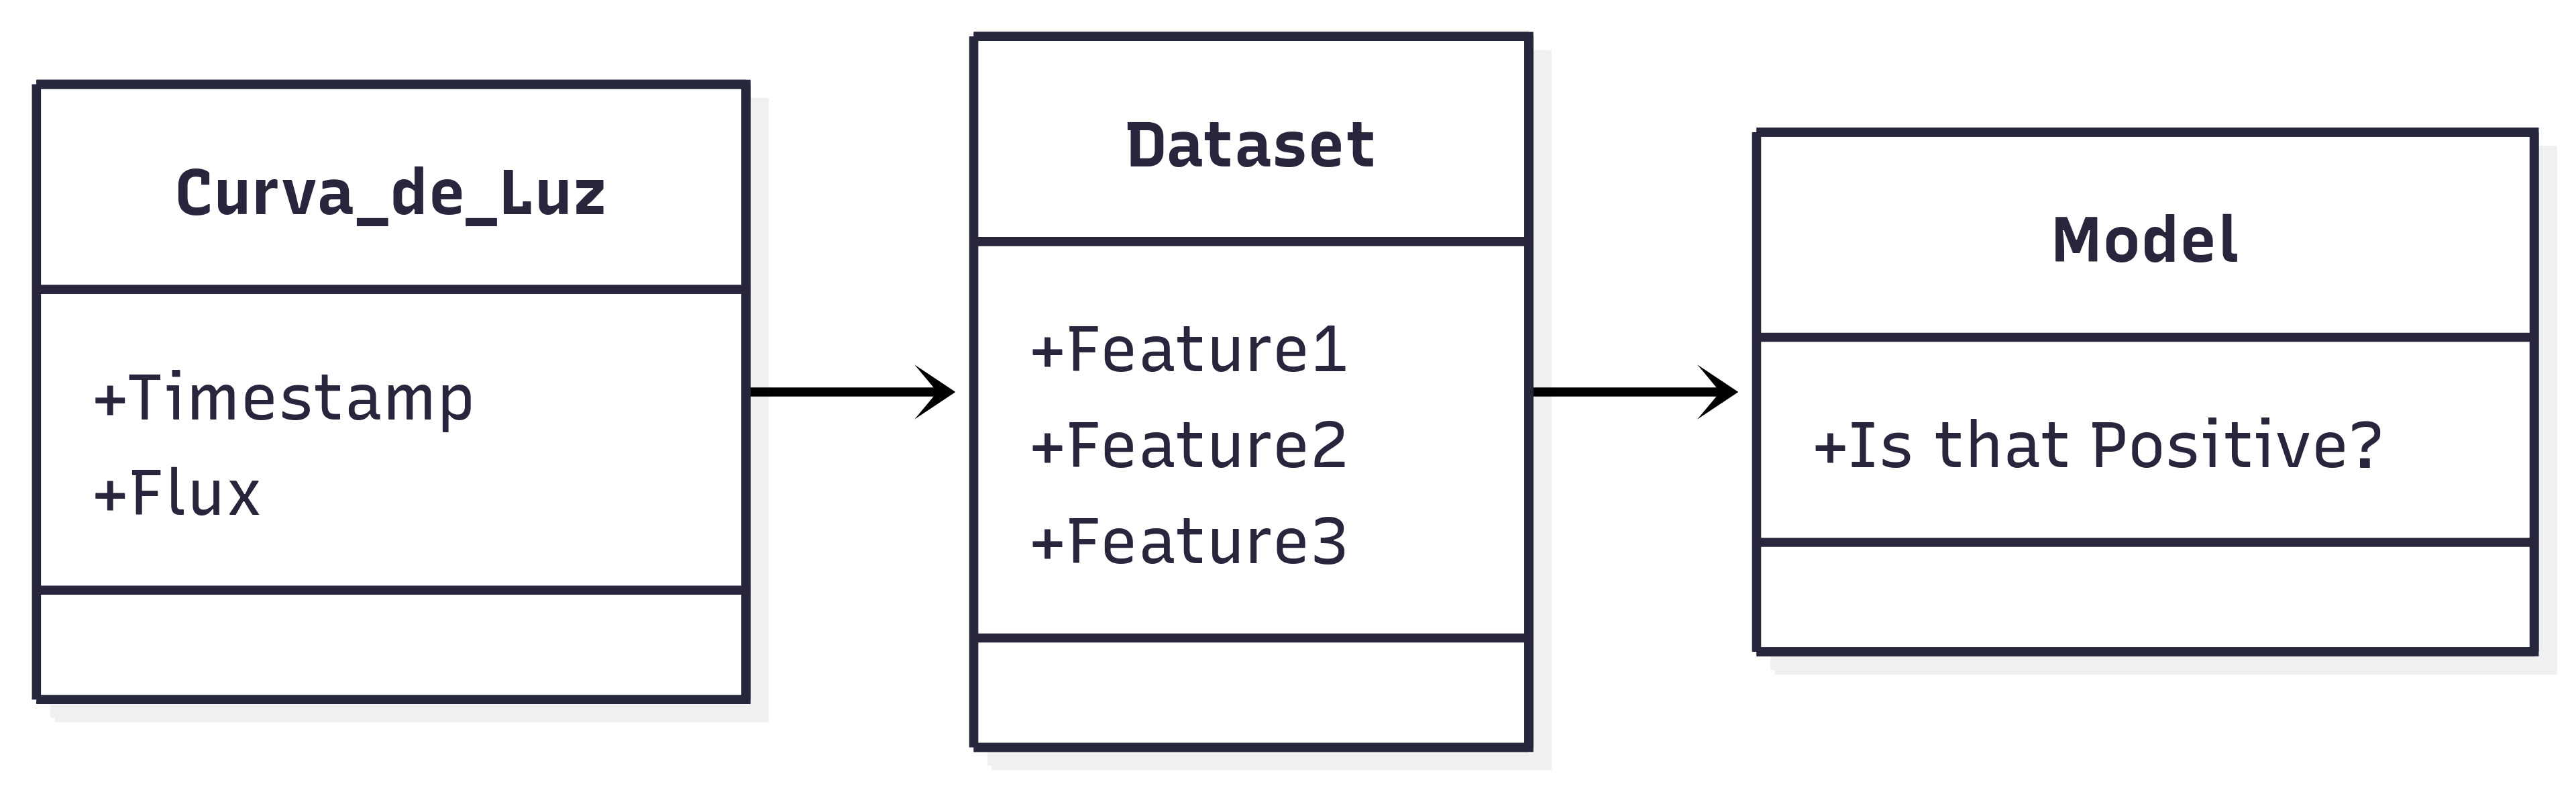
\includegraphics[scale=0.08]{pngs/diagrama_1.png}
\caption{Esquema da \textit{pipeline}: as curvas de luz são convertidas em vetores de características; o treinamento utiliza essas características, e não as séries temporais brutas.}
\label{fig:diagrama_pipeline}
\end{center}
\end{figure}

% -----------------------------------------------------------------------------
\section{Aquisição e armazenamento dos dados}
\label{sec:aquisição}

\subsection{Fontes de dados}

As curvas de luz utilizadas neste trabalho provêm de duas origens principais.

\textbf{Grupo do Rio:} parte do conjunto foi obtida a partir do banco de dados em nuvem do Grupo do Rio, referente a campanhas de ocultações já analisadas na literatura: ocultação por Umbriel (satélite de Urano), observada em 2020 e analisada por \cite{Umbriel2020}, e ocultação por Chiron, \DIFdelbegin \DIFdel{observada em 2023 e }\DIFdelend analisada por \cite{Chiron2023}. Esses dados já possuem classificação (positiva ou negativa) e metadados consistentes. \DIFaddbegin \DIFadd{A observação de Chiron, porém, está registrada no banco sem pontos de curva de luz e não entrou no conjunto de dados; na prática, a contribuição do Grupo do Rio ao conjunto restringe-se às cordas de Umbriel.
}\DIFaddend 

\textbf{VizieR:} a maior parte das curvas foi adquirida no portal VizieR (\textit{cdsarc.cds.unistra.fr}), catálogo \texttt{B/occ/asteroid} \DIFaddbegin \DIFadd{\mbox{%DIFAUXCMD
\citep{HeraldBocc2016}}\hskip0pt%DIFAUXCMD
}\DIFaddend , totalizando centenas de curvas em formato \texttt{.dat}, contendo séries temporais de tempo e fluxo. Para cada entrada do catálogo, os pontos da curva são baixados via serviço \texttt{vizgraph} e armazenados localmente. Convém esclarecer uma possível confusão de escalas: os milhares de registros mencionados na Introdução referem-se às \textbf{imagens (quadros)} que cada observação produz, das quais se extrai \emph{uma} curva de luz por fotometria. O conjunto de dados deste trabalho é contado em \textbf{curvas}, não em quadros --- são centenas de curvas, que, somadas \DIFdelbegin \DIFdel{aos negativos por recorte e }\DIFdelend às curvas \DIFdelbegin \DIFdel{sintéticas}\DIFdelend \DIFaddbegin \DIFadd{negativas (cuja obtenção é descrita na Seção~\ref{sec:construcao_dataset})}\DIFaddend , totalizam as 1693 amostras detalhadas na Seção~\ref{sec:config_experimental} (Capítulo~5).

O processamento e a integração dos dados foram realizados com as bibliotecas \texttt{Astropy} \DIFaddbegin \DIFadd{\mbox{%DIFAUXCMD
\citep{Astropy2022} }\hskip0pt%DIFAUXCMD
}\DIFaddend e \texttt{Astroquery} \DIFaddbegin \DIFadd{\mbox{%DIFAUXCMD
\citep{Astroquery2019} }\hskip0pt%DIFAUXCMD
}\DIFaddend (leitura e consulta a catálogos astronômicos), \texttt{asyncio} \DIFaddbegin \DIFadd{(biblioteca padrão do Python) }\DIFaddend e \texttt{aiohttp} (coleta assíncrona, reduzindo o tempo total de aquisição), e \texttt{Pandas} \DIFaddbegin \DIFadd{\mbox{%DIFAUXCMD
\citep{McKinney2010} }\hskip0pt%DIFAUXCMD
}\DIFaddend (manipulação tabular). \DIFdelbegin \DIFdel{Scripts }\DIFdelend \DIFaddbegin \DIFadd{As rotinas numéricas de suavização e de testes estatísticos (Seção~\ref{sec:features}) usam a biblioteca SciPy \mbox{%DIFAUXCMD
\citep{SciPy2020}}\hskip0pt%DIFAUXCMD
. }\textit{\DIFadd{Scripts}} \DIFaddend em Python foram desenvolvidos para automatizar a busca, o \DIFdelbegin \DIFdel{download }\DIFdelend \DIFaddbegin \textit{\DIFadd{download}} \DIFaddend e a organização dos arquivos.

Vale observar nos fluxogramas (Figuras~\ref{fig:fluxo1} e~\ref{fig:fluxo2}) um detalhe do procedimento: as curvas do VizieR foram baixadas e \textbf{triadas localmente} --- com \DIFaddbegin \DIFadd{pré-visualizações (}\DIFaddend \textit{previews}\DIFaddbegin \DIFadd{) }\DIFaddend em \texttt{.png} e arquivos \texttt{.dat} organizados em pastas --- antes de um \textit{script} de importação inseri-las no banco. Essa triagem prévia agilizou a inspeção de centenas de curvas que poderiam não ser positivas, estar em formato divergente ou sequer ser curvas de luz (por exemplo, curvas de rotação). Como efeito colateral, essas curvas foram registradas com origem \emph{local}, de modo que nenhuma observação consta explicitamente como \texttt{VizieR} no campo de origem --- um detalhe de proveniência corrigível por uma simples consulta SQL e sem efeito sobre os rótulos positivo/negativo. Registra-se, ainda, que as curvas marcadas como defeituosas no \textit{download} foram descartadas sem caracterização do defeito nem tentativa de reaproveitamento (decisão de escopo e tempo que constitui uma fragilidade reconhecida da metodologia).

\begin{figure}[htbp]
\begin{center}
	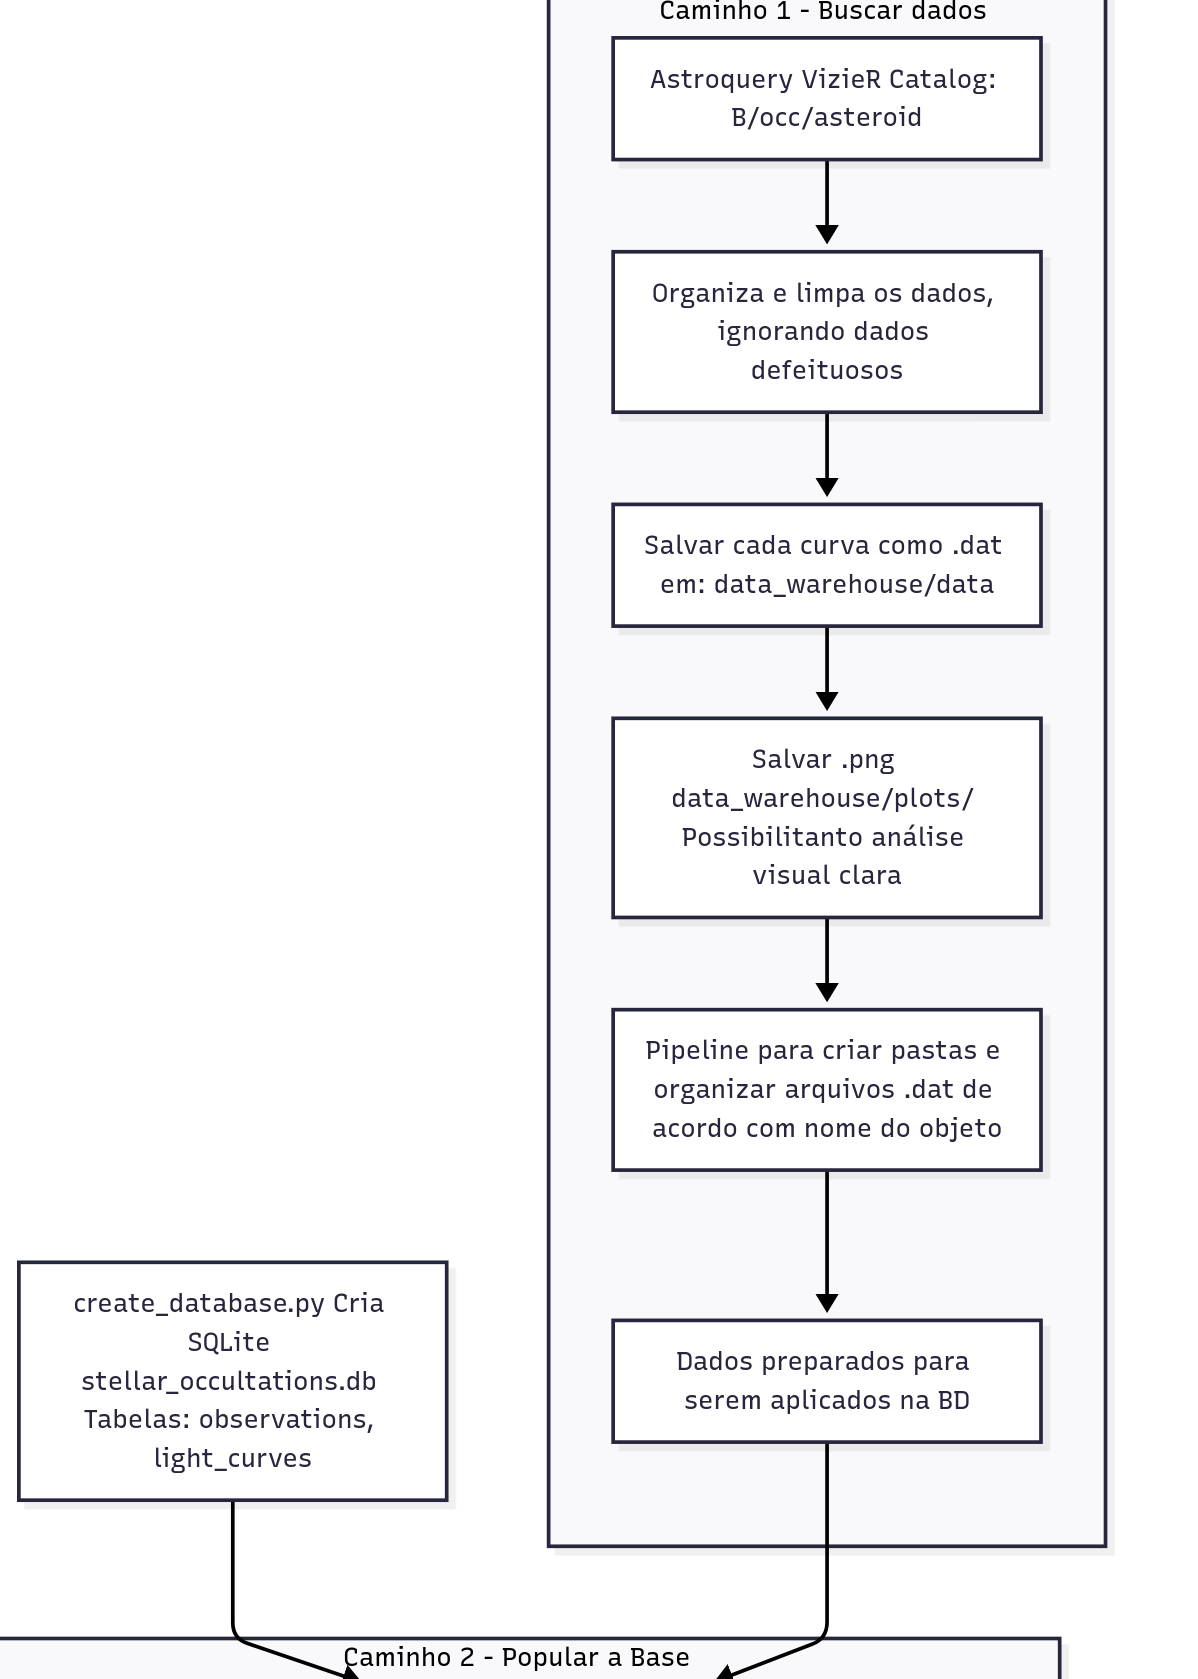
\includegraphics[scale=0.3]{pngs/fluxo1.png}
\caption{Fluxograma da aquisição e organização dos dados externos e da integração na etapa de inserção no banco de dados.}
\label{fig:fluxo1}
\end{center}
\end{figure}

\subsection{Estrutura do banco de dados}

O banco de dados relacional foi implementado em SQLite (\texttt{.db}) e estruturado em duas tabelas principais, garantindo integridade referencial e consultas eficientes.

\textbf{Tabela \texttt{observations}:} armazena informações gerais de cada observação: identificador único, nome do objeto ocultador, data da observação, portal de origem, nome do observador e metadados adicionais (incluindo a classificação do evento como ocultação positiva ou negativa, quando disponível).

\textbf{Tabela \texttt{light\_curves}:} contém os pontos individuais de cada curva de luz (tempo e fluxo), vinculados à observação correspondente por uma chave estrangeira (\texttt{observation\_id}). Assim, uma mesma observação pode possuir muitos pontos, mantendo a normalização do esquema.

Durante a inserção, buscou-se preservar ao máximo os valores originais, realizando apenas ajustes mínimos de consistência: \DIFdelbegin \DIFdel{uniformização de unidades quando necessário, }\DIFdelend checagem do alinhamento temporal e validação de metadados, sem alterar as características intrínsecas das curvas. \DIFdelbegin \DIFdel{A }\DIFdelend \DIFaddbegin \DIFadd{Os tempos foram armazenados na unidade fornecida por cada fonte: segundos nas curvas do VizieR e dias julianos nas do Grupo do Rio. A diferença só afeta a característica de duração do evento, convertida para segundos antes do treinamento (Capítulo~5). A }\DIFaddend Figura~\ref{fig:fluxo2} resume o fluxo de consolidação do banco.

\begin{figure}[htbp]
\begin{center}
	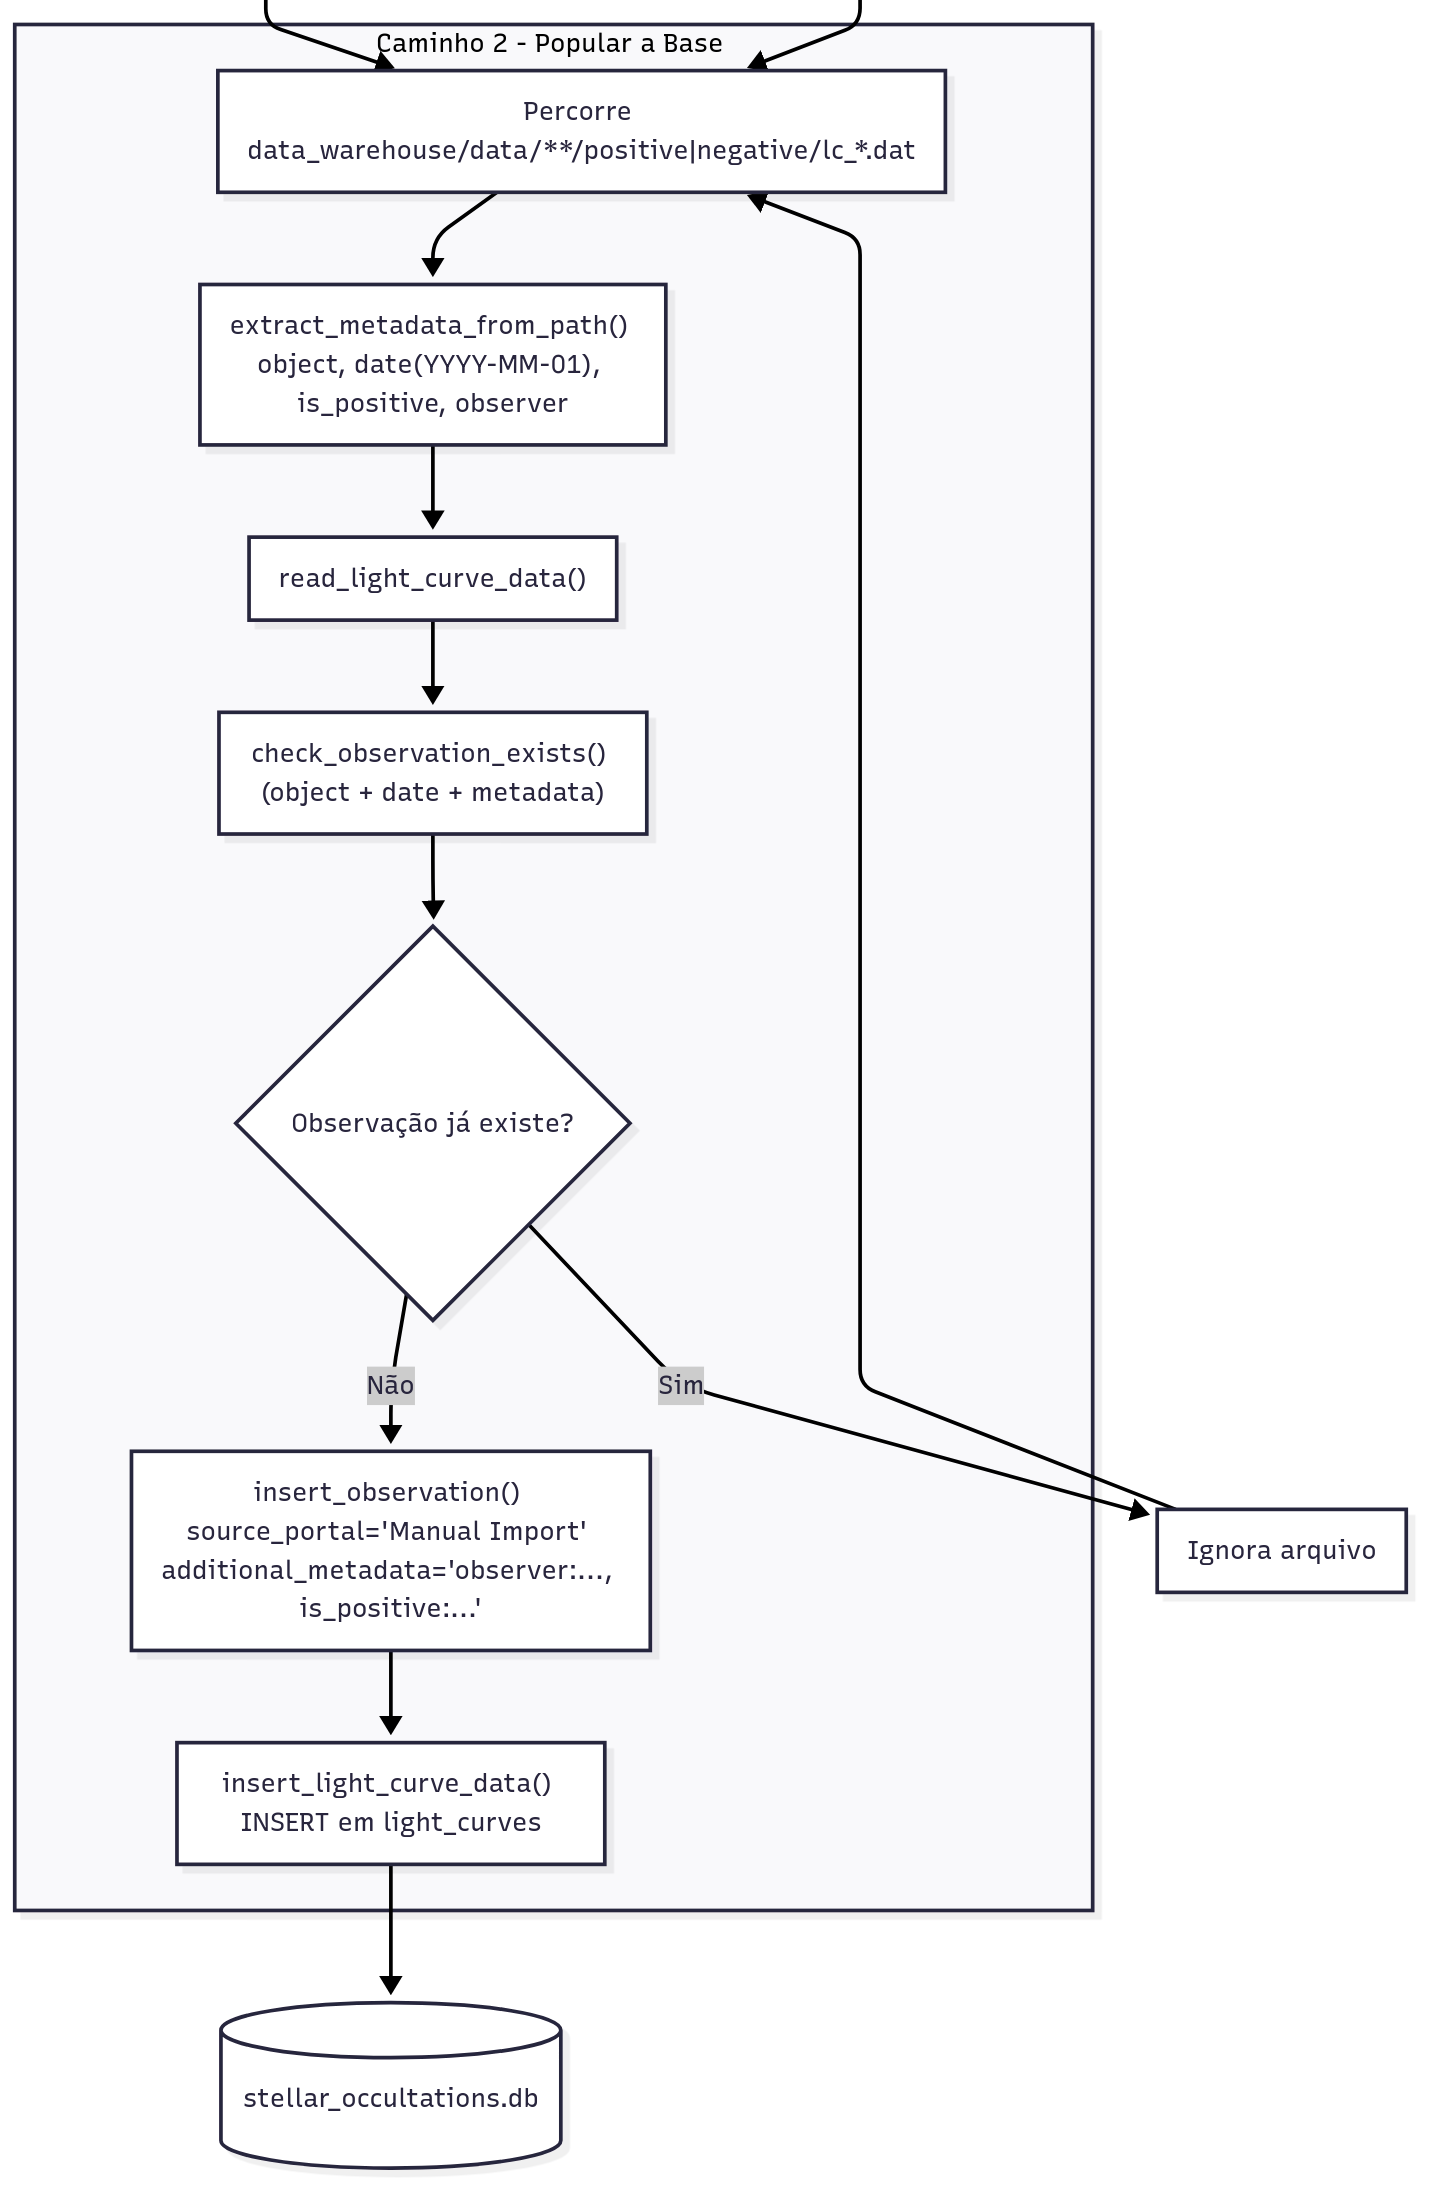
\includegraphics[scale=0.3]{pngs/fluxo2.png}
\caption{Fluxograma da \textit{pipeline} responsável pela consolidação do banco de dados.}
\label{fig:fluxo2}
\end{center}
\end{figure}

% -----------------------------------------------------------------------------
\section{Acesso aos dados e normalização}
\label{sec:acesso}

Após a consolidação no banco, um módulo dedicado (\textit{data access}) é responsável por consultar as curvas, filtrá-las por critérios (objeto, data, tipo positivo/negativo) e prepará-las para as etapas seguintes.

\subsection{Consulta e classificação}

As curvas são identificadas como \textbf{positivas} (com evento de ocultação) ou \textbf{negativas} (sem evento) com base em metadados armazenados na tabela \texttt{observations} (campo de metadados adicionais). Essa classificação pode provir de análises prévias (como no caso do Grupo do Rio) ou de anotações inseridas durante a organização dos dados. No Grupo do Rio, os rótulos decorrem das análises publicadas nas campanhas citadas (Umbriel, Chiron), realizadas por especialistas do grupo; no VizieR, a classificação positiva/negativa provém dos curadores do catálogo \texttt{B/occ/asteroid}. Não há estudo formal de concordância entre anotadores neste trabalho; as métricas de desempenho reportadas no Capítulo 5 são, portanto, relativas a esse \textit{ground truth} e devem ser lidas com a ressalva de que erros ou inconsistências de rotulagem nos catálogos podem afetar tanto o treinamento quanto a avaliação dos modelos. Durante a organização dos dados não foram identificados casos confirmados de rótulo invertido (positiva rotulada como negativa ou vice-versa); contudo, como não se realizou uma reanálise independente de cada curva, não é possível descartar a existência de inconsistências pontuais herdadas dos catálogos de origem. O módulo de acesso permite listar objetos disponíveis, datas de observação por objeto e, para cada par objeto--data, recuperar as curvas com seus rótulos.

\subsection{Normalização do fluxo}

O fluxo fotométrico bruto varia em escala entre observações (diferentes telescópios, condições de céu, etc.). Para colocar todas as curvas em uma base comparável, aplica-se uma normalização que estima um \textit{baseline} (nível de fluxo fora da ocultação) e divide-se a série pelo valor desse \DIFdelbegin \DIFdel{baseline}\DIFdelend \DIFaddbegin \textit{\DIFadd{baseline}}\DIFaddend .

A estratégia adotada é a seguinte: a série temporal do fluxo é dividida em quatro segmentos contíguos (quartis em ordem temporal). Calcula-se a média de cada segmento; os dois segmentos com maior média são considerados representativos do nível fora da ocultação. O \textit{baseline} é definido como a média dessas duas médias. O fluxo inteiro é então dividido por esse \DIFdelbegin \DIFdel{baseline}\DIFdelend \DIFaddbegin \textit{\DIFadd{baseline}}\DIFaddend , de modo que, em curvas sem ocultação ou nos trechos externos à ocultação, o valor normalizado fique próximo de 1. Em curvas com ocultação, a região de queda aparece com valores inferiores a 1. Em casos degenerados (poucos pontos ou \DIFdelbegin \DIFdel{baseline }\DIFdelend \DIFaddbegin \textit{\DIFadd{baseline}} \DIFaddend inválido), recorre-se à média global do fluxo como alternativa. A normalização coloca todas as curvas em uma escala comparável, facilitando a convergência dos algoritmos e a interpretação de resíduos; em modelos de regressão, a análise de resíduos é um diagnóstico fundamental para verificar a aderência do modelo aos dados \citep{Morettin2010}. Esse procedimento é análogo a uma normalização ``pós-fotometria'', em que o nível de continuum já foi tratado.

\subsection{Remoção de \textit{outliers}}

Quando necessário, pontos extremos do fluxo podem ser removidos com base em um critério de z-score: para um limiar \(z_{\mathrm{lim}}\) (por exemplo, 3), pontos cujo fluxo se afasta da média da série por mais de \(z_{\mathrm{lim}}\) desvios padrão são descartados. Isso reduz o impacto de picos ou quedas espúrias pontuais (defeitos de leitura, raios cósmicos, etc.) sem alterar a estrutura geral da curva.

% -----------------------------------------------------------------------------
\DIFaddbegin \let\oldsectionmark\sectionmark %DIF >  cabeçalho de página curto só nesta seção (o título completo não cabe)
\renewcommand{\sectionmark}[1]{\oldsectionmark{Construção do conjunto de dados}}
\DIFaddend \section{Construção do conjunto de dados para aprendizado de máquina}
\DIFaddbegin \let\sectionmark\oldsectionmark
\DIFaddend \label{sec:construção_dataset}
\DIFaddbegin \label{sec:construcao_dataset}
\DIFaddend 

O \textbf{conjunto de dados} (\DIFdelbegin \DIFdel{dataset}\DIFdelend \DIFaddbegin \textit{\DIFadd{dataset}}\DIFaddend ) é a tabela de exemplos (curvas de luz convertidas em vetores de características) com sua\DIFdelbegin \DIFdel{s}\DIFdelend  classificação verdadeira (positiva ou negativa), usada para treinar e avaliar os classificadores. Devido à escassez de curvas negativas nos catálogos disponíveis, adotaram-se duas estratégias complementares: recorte de segmentos sem ocultação a partir de curvas positivas e geração de curvas \DIFdelbegin \DIFdel{sintéticas negativas }\DIFdelend \DIFaddbegin \DIFadd{negativas simuladas }\DIFaddend com o simulador \DIFdelbegin \DIFdel{físico de Gomes-Ferrante \& Braga-Ribas~\mbox{%DIFAUXCMD
\citep{Simulator}}\hskip0pt%DIFAUXCMD
}\DIFdelend \DIFaddbegin \DIFadd{de curvas de luz de ocultação de \mbox{%DIFAUXCMD
\citet{Simulator}}\hskip0pt%DIFAUXCMD
}\DIFaddend . Os detalhes de cada estratégia são descritos nas subseções seguintes.

\subsection{Tamanho e composição do conjunto de dados}

Para interpretar sobreajuste, significância das métricas e generalização no Capítulo 5, é essencial conhecer o tamanho e a composição do conjunto utilizado. A composição final (quantidade de curvas positivas, negativas do banco, negativos por recorte manual, curvas \DIFdelbegin \DIFdel{sintéticas}\DIFdelend \DIFaddbegin \DIFadd{simuladas}\DIFaddend , total de amostras e proporção treino/teste) é apresentada na Seção~\ref{sec:config_experimental} (\DIFdelbegin \DIFdel{Configuração }\DIFdelend \DIFaddbegin \DIFadd{Protocolo }\DIFaddend experimental), onde os números dos experimentos são detalhados junto com a distribuição por fonte.

\subsection{Curvas positivas e negativas do banco}

As curvas classificadas como positivas são obtidas do banco via consultas que filtram observações com rótulo correspondente. As curvas negativas são obtidas da mesma forma. O número de curvas negativas ``nativas'' (observações realmente sem ocultação) costuma ser menor que o de positivas \DIFdelbegin \DIFdel{em muitos catálogos}\DIFdelend \DIFaddbegin \DIFadd{no catálogo utilizado neste trabalho}\DIFaddend . Além disso, o catálogo obtido via VizieR, que constitui a principal fonte de dados deste trabalho, contém exclusivamente curvas positivas.

\subsection{Recorte de segmentos negativos a partir de curvas positivas}

Uma estratégia para obter exemplos negativos de alta qualidade consiste em extrair, das próprias curvas positivas, os trechos localizados \textbf{fora} da região de ocultação (isto é, anteriores à imersão e posteriores à emersão). Esses segmentos representam observações do mesmo sinal na ausência do evento e, portanto, constituem candidatos adequados para compor a classe negativa (denominados \textbf{negativos por recorte}). Contudo, por serem derivados da mesma curva de luz \DIFaddbegin \DIFadd{de ocultação, os recortes compartilham com ela a mesma estrela (brilho, cor e diâmetro aparente), o mesmo instrumento e as mesmas condições de imagem daquela noite (PSF, }\textit{\DIFadd{seeing}}\DIFaddend , \DIFdelbegin \DIFdel{compartilham características intrínsecas da observação, como instrumentação}\DIFdelend \DIFaddbegin \DIFadd{cadência}\DIFaddend , \DIFdelbegin \DIFdel{condições observacionais e propriedades da estrela observada. Assim, para evitar vazamento de informação (}\textit{\DIFdel{data leakage}}%DIFAUXCMD
\DIFdel{) e reduzir o risco de viés nos modelos, a curva positiva que originou os recortes deve ser removida do conjunto de dados utilizado no treinamento e na avaliação}\DIFdelend \DIFaddbegin \DIFadd{cintilação e transparência)}\DIFaddend .

O procedimento adotado foi o seguinte: \DIFdelbegin \DIFdel{para }\DIFdelend \DIFaddbegin \DIFadd{em }\DIFaddend cada curva positiva \DIFdelbegin \DIFdel{simples, identifica-se }\DIFdelend \DIFaddbegin \DIFadd{de uma amostra aleatória, }\DIFaddend a região de ocultação \DIFdelbegin \DIFdel{de forma manual. Os segmentos antes e depois dessa }\DIFdelend \DIFaddbegin \DIFadd{é delimitada automaticamente pelo primeiro e pelo último ponto com fluxo normalizado inferior a 0,78, após a remoção de }\textit{\DIFadd{outliers}} \DIFadd{a \(3\sigma\); os segmentos anterior e posterior a essa }\DIFaddend região\DIFaddbegin \DIFadd{, com pelo menos 20 pontos cada, }\DIFaddend são \DIFdelbegin \DIFdel{recortados. Quando isso ocorre}\DIFdelend \DIFaddbegin \DIFadd{exibidos e aceitos ou rejeitados manualmente. Se ao menos um segmento é aceito}\DIFaddend , a curva positiva original é excluída do conjunto de \DIFdelbegin \DIFdel{positivos usados no treino, para evitar }\DIFdelend \DIFaddbegin \DIFadd{positivas, para }\DIFaddend que a mesma observação \DIFaddbegin \DIFadd{não }\DIFaddend apareça \DIFdelbegin \DIFdel{tanto como positiva quanto }\DIFdelend como \DIFaddbegin \DIFadd{positiva e como }\DIFaddend negativa (vazamento de informação\DIFdelbegin \DIFdel{)}\DIFdelend \DIFaddbegin \DIFadd{, ou }\textit{\DIFadd{data leakage}}\DIFadd{). Pelo mesmo motivo, nas partições de treino, validação e teste (Capítulo~5), os recortes de uma mesma curva e as demais cordas do mesmo evento formam um único grupo, que nunca é dividido entre os dois lados de uma partição. Quedas rasas que não cruzam o limiar de 0,78 --- como as de anéis, atmosferas ou ocultações rasantes --- não são detectadas por esse critério e, se presentes fora do evento principal, permanecem nos segmentos rotulados como negativos; a inspeção visual é a única salvaguarda}\DIFaddend .
\DIFdelbegin \DIFdel{Essa abordagem reduz o risco de viés e garante que os negativos por recorte correspondam de fato a trechos sem ocultação.
}\DIFdelend 

\subsection{Curvas \DIFdelbegin \DIFdel{sintéticas }\DIFdelend negativas \DIFaddbegin \DIFadd{simuladas}\DIFaddend }

Para diversificar ainda mais a classe negativa e cobrir condições variadas de ruído e amostragem, foram incorporadas \textbf{curvas de luz \DIFdelbegin \DIFdel{sintéticas}\DIFdelend \DIFaddbegin \DIFadd{simuladas}\DIFaddend } geradas por um simulador físico \citep{Simulator}. O simulador combina: (i)~\DIFaddbegin \DIFadd{a }\DIFaddend geometria do evento \DIFdelbegin \DIFdel{(tempo, }\DIFdelend \DIFaddbegin \DIFadd{--- o instante de cada exposição é convertido na }\DIFaddend posição \DIFaddbegin \DIFadd{do observador }\DIFaddend ao longo da corda\DIFdelbegin \DIFdel{); }\DIFdelend \DIFaddbegin \DIFadd{, \(x(t) = V_S\,(t-t_0)\), medida no plano do céu a partir do centro do evento; o corpo é representado por uma faixa opaca de largura igual ao seu diâmetro, o que equivale a uma corda central; }\DIFaddend (ii)~\DIFaddbegin \DIFadd{a }\DIFaddend difração de Fresnel nas bordas de imersão e emersão\DIFaddbegin \DIFadd{, o diâmetro aparente da estrela e a integração durante a exposição}\DIFaddend ; (iii)~\DIFaddbegin \DIFadd{um }\DIFaddend modelo de ruído \DIFdelbegin \DIFdel{(Poisson}\DIFdelend \DIFaddbegin \DIFadd{branco (Poisson da estrela e do céu}\DIFaddend , ruído de leitura \DIFdelbegin \DIFdel{, }\DIFdelend \DIFaddbegin \DIFadd{gaussiano e }\DIFaddend cintilação \DIFdelbegin \DIFdel{atmosférica}\DIFdelend \DIFaddbegin \DIFadd{multiplicativa lognormal}\DIFaddend ); (iv)~\DIFaddbegin \DIFadd{a }\DIFaddend normalização pós-fotometria. Para a classe negativa, \DIFdelbegin \DIFdel{são geradas curvas sem evento (ou com }\DIFdelend \DIFaddbegin \DIFadd{o }\DIFaddend diâmetro \DIFdelbegin \DIFdel{efetivo nulo)}\DIFdelend \DIFaddbegin \DIFadd{é nulo: a geometria e a difração não intervêm, e cada curva simulada consiste apenas na base de tempo (20 a 60\,s de duração, com exposições de 0}\DIFaddend ,\DIFdelbegin \DIFdel{submetidas ao mesmo tipo de }\DIFdelend \DIFaddbegin \DIFadd{05 a 0,25\,s) e no ruído, com parâmetros sorteados uniformemente (estrela de magnitude 11 a 14,5; }\textit{\DIFadd{seeing}} \DIFadd{de \(0{,}8''\) a \(1{,}6''\)). Não foram incluídos }\DIFaddend ruído \DIFdelbegin \DIFdel{e normalização das curvas reais}\DIFdelend \DIFaddbegin \DIFadd{correlacionado, variações de transparência nem nuvens}\DIFaddend . As curvas \DIFdelbegin \DIFdel{sintéticas }\DIFdelend \DIFaddbegin \DIFadd{simuladas }\DIFaddend são exportadas em formato \texttt{.dat} e carregadas pelo módulo de construção do \DIFdelbegin \DIFdel{dataset}\DIFdelend \DIFaddbegin \textit{\DIFadd{dataset}}\DIFaddend , sendo tratadas como negativas. Essa etapa permite aumentar o tamanho e a variedade do conjunto de treino\DIFdelbegin \DIFdel{e melhorar a generalização do modelo em condições diversas}\DIFdelend \DIFaddbegin \DIFadd{. Por construção, porém, o ruído simulado é em geral menor que o das curvas observadas: a mediana do desvio padrão fora do evento (}\texttt{\DIFadd{Occ\_baseline\_std}}\DIFadd{) é 0,021 nas negativas simuladas, contra 0,058 nos negativos por recorte e 0,104 nas positivas. Por isso o desempenho é avaliado também somente em curvas reais (Capítulo~5)}\DIFaddend .

O conjunto final reúne, portanto: positivas do banco (excluindo as usadas para recorte), negativas do banco, negativos por recorte (segmentos recortados e aprovados) e curvas \DIFdelbegin \DIFdel{sintéticas negativas }\DIFdelend \DIFaddbegin \DIFadd{negativas simuladas}\DIFaddend . Cabe destacar que o catálogo \texttt{B/occ/asteroid} do VizieR, principal fonte das curvas positivas, é um agregador público de campanhas independentes envolvendo diferentes corpos, observadores, telescópios, datas e localizações geográficas; a diversidade observacional do conjunto positivo é, portanto, \DIFdelbegin \DIFdel{intrínseca à natureza do catálogo, e não há fonte observacional única que possa enviesar essa classe}\DIFdelend \DIFaddbegin \DIFadd{considerável, embora alguns eventos e observadores contribuam com várias curvas (por exemplo, 11 cordas positivas de Umbriel)}\DIFaddend . Os pontos onde existe acoplamento entre amostras são explicitamente assumidos e mitigados: (i)~os negativos por recorte herdam telescópio, estrela e noite da curva positiva da qual foram recortados, motivo pelo qual a positiva original é excluída do conjunto \DIFdelbegin \DIFdel{de treino}\DIFdelend \DIFaddbegin \DIFadd{e todas as curvas de um mesmo evento são mantidas juntas nas partições}\DIFaddend ; (ii)~as curvas \DIFdelbegin \DIFdel{sintéticas}\DIFdelend \DIFaddbegin \DIFadd{simuladas}\DIFaddend , geradas por simulador físico, \DIFdelbegin \DIFdel{podem apresentar }\DIFdelend \DIFaddbegin \DIFadd{apresentam }\DIFaddend características de ruído distintas das observações reais, limitação \DIFdelbegin \DIFdel{retomada e quantificada no Experimento~3 (}\DIFdelend \DIFaddbegin \DIFadd{avaliada pela taxa de falsos positivos nas negativas reais e pela avaliação restrita a curvas reais (Análise~2.1, }\DIFaddend Capítulo~5). \DIFaddbegin \DIFadd{A Figura~\ref{fig:exemplos_curvas} mostra exemplos de cada tipo de curva do conjunto. }\DIFaddend Todas as curvas passam pela mesma etapa de extração de características, descrita na próxima seção.

\DIFaddbegin \begin{figure}[htbp]
\centering
\includegraphics[width=0.95\linewidth]{Tese/pngs/reanalise/exemplos_curvas.png}
\caption{\DIFaddFL{Exemplos de curvas de luz do conjunto de dados, com o fluxo normalizado pela média dos dois quartis temporais mais altos: (a)~positiva com queda profunda; (b)~positiva com queda parcial e ruído alto; (c)~negativa real (corda negativa da campanha de Umbriel), justamente a negativa real que o XGBoost classifica como positiva no conjunto de teste (Seção~\ref{sec:teste_final}); (d)~exemplo de negativa simulada gerado com o simulador, sem corpo ocultante (estrela de magnitude 13, exposição de 0,1~s, 40~s de registro); não é uma das 702 curvas do conjunto. Os rótulos de (a)--(c) indicam objeto, mês e ano de observação e observador.}}
\label{fig:exemplos_curvas}
\end{figure}

\DIFaddend % -----------------------------------------------------------------------------
\section{Engenharia de características}
\label{sec:features}

\DIFdelbegin \DIFdel{As curvas de luz são séries temporais (tempo \(\times\) fluxo). }\DIFdelend Os modelos de classificação utilizados neste trabalho (Regressão Logística, Random Forest, XGBoost, CatBoost) recebem \textbf{vetores numéricos}, \DIFaddbegin \DIFadd{e }\DIFaddend não as séries brutas\DIFdelbegin \DIFdel{. Por }\DIFdelend \DIFaddbegin \DIFadd{; por }\DIFaddend isso, cada curva é convertida \DIFdelbegin \DIFdel{em um vetor de }\textbf{\DIFdel{características}} %DIFAUXCMD
\DIFdel{(features) extraídas da série --- por exemplo, amplitude, mínimo do fluxo suavizado, distância entre centróides do K-means, etc. O resultado é uma tabela em que cada linha é uma curva e cada coluna é uma dessas grandezas. }\DIFdelend \DIFaddbegin \DIFadd{no vetor de características descrito nesta seção. }\DIFaddend As características foram padronizadas (média zero, desvio unitário) \textbf{apenas para a Regressão Logística}, via \texttt{StandardScaler} --- o transformador da biblioteca \texttt{scikit-learn} \citep{ScikitLearn2011} que, para cada variável, subtrai a média e divide pelo desvio padrão do conjunto de treino ---, uma vez que a regularização $\ell_2$ é sensível à escala das variáveis \citep{geron2019maos}. Os modelos baseados em árvores (Random Forest, XGBoost, CatBoost) recebem as \textit{features} em escala original, pois são insensíveis a transformações monotônicas de cada variável.

\DIFdelbegin \DIFdel{Adiante veremos que algumas }\DIFdelend \DIFaddbegin \DIFadd{Algumas das }\DIFaddend características extraídas \DIFdelbegin \DIFdel{carregarão informações redundantes . Isto }\DIFdelend \DIFaddbegin \DIFadd{são redundantes entre si. Isso }\DIFaddend é proposital \DIFdelbegin \DIFdel{, pois motivará uma demonstração sobre }\DIFdelend \DIFaddbegin \DIFadd{e permite avaliar, no Capítulo~5, o efeito da }\DIFaddend redução \DIFdelbegin \DIFdel{de dimensionalidade nos modelosfinais}\DIFdelend \DIFaddbegin \DIFadd{do conjunto de variáveis sobre o desempenho dos modelos}\DIFaddend .

\subsection{\DIFdelbegin \DIFdel{Estatísticas básicas }\DIFdelend \DIFaddbegin \DIFadd{Amplitude e desvio padrão }\DIFaddend do fluxo}

Seja \(F(t)\) a série de fluxo (preferencialmente normalizado) com \(N\) pontos. Definem-se:

\begin{equation}
\DIFdelbegin \DIFdel{\mu }\DIFdelend \DIFaddbegin \hat{\mu} \DIFaddend = \frac{1}{N} \sum_{i=1}^{N} F(t_i), \qquad
\DIFdelbegin \DIFdel{\sigma }\DIFdelend \DIFaddbegin \hat{\sigma} \DIFaddend = \DIFdelbegin \DIFdel{\sqrt{\frac{1}{N - 1} \sum_{i=1}^{N} \left( F(t_i) - \mu \right)^2}}\DIFdelend \DIFaddbegin \DIFadd{\sqrt{\frac{1}{N - 1} \sum_{i=1}^{N} \left( F(t_i) - \hat{\mu} \right)^2}}\DIFaddend ,
\end{equation}

\begin{equation}
F_{\min} = \min_{1 \leq i \leq N} F(t_i), \qquad
F_{\max} = \max_{1 \leq i \leq N} F(t_i).
\end{equation}

A amplitude da curva é \(\mathrm{Amp} = F_{\max} - F_{\min}\). Em curvas com ocultação, a amplitude tende a ser maior (queda pronunciada); em curvas \DIFdelbegin \DIFdel{apenas ruidosas, \(\sigma\) }\DIFdelend \DIFaddbegin \DIFadd{negativas, o desvio padrão (\(\hat{\sigma}\)) }\DIFaddend e a amplitude \DIFdelbegin \DIFdel{podem }\DIFdelend \DIFaddbegin \DIFadd{tendem a }\DIFaddend ser menores. \DIFaddbegin \DIFadd{Os acentos circunflexos indicam que \(\hat{\mu}\) e \(\hat{\sigma}\) são estimativas, calculadas a partir dos \(N\) pontos da curva, da média e do desvio padrão do fluxo. }\DIFaddend O desvio padrão \DIFdelbegin \DIFdel{\(\sigma\) }\DIFdelend \DIFaddbegin \DIFadd{\(\hat{\sigma}\) }\DIFaddend e a amplitude são portanto candidatos naturais a \textit{features} discriminativas.

\subsection{Suavização \DIFdelbegin \DIFdel{e médias móveis}\DIFdelend \DIFaddbegin \DIFadd{(filtro de Savitzky-Golay)}\DIFaddend }
\DIFaddbegin \label{sec:suavizacao}
\DIFaddend 

Para reduzir o ruído de alta frequência sem perder a forma geral da curva, aplica-se uma \DIFdelbegin \DIFdel{janela de }\DIFdelend suavização. \DIFdelbegin \DIFdel{A suavização }\DIFdelend \DIFaddbegin \DIFadd{Ela }\DIFaddend atua como um filtro passa-baixa \DIFdelbegin \DIFdel{: atenua as flutuações }\DIFdelend \DIFaddbegin \DIFadd{--- um filtro que deixa passar as variações lentas (baixas frequências) e atenua as }\DIFaddend rápidas \DIFaddbegin \DIFadd{(altas frequências): as flutuações }\DIFaddend ponto a ponto\DIFdelbegin \DIFdel{(componentes de alta frequência, associadas ao }\DIFdelend \DIFaddbegin \DIFadd{, dominadas pelo }\DIFaddend ruído\DIFdelbegin \DIFdel{) e preserva }\DIFdelend \DIFaddbegin \DIFadd{, são atenuadas, enquanto }\DIFaddend as variações lentas\DIFdelbegin \DIFdel{(baixa frequência)}\DIFdelend , que descrevem a forma da ocultação\DIFdelbegin \DIFdel{. A janela }\DIFdelend \DIFaddbegin \DIFadd{, são preservadas. Utiliza-se o filtro de Savitzky-Golay \mbox{%DIFAUXCMD
\citep{SavitzkyGolay1964}}\hskip0pt%DIFAUXCMD
, implementado na função }\texttt{\DIFadd{savgol\_filter}} \DIFadd{da biblioteca SciPy \mbox{%DIFAUXCMD
\citep{SciPy2020}}\hskip0pt%DIFAUXCMD
: em cada janela móvel de \(w\) pontos ajusta-se, por mínimos quadrados, um polinômio de grau 2, e o ponto central }\DIFaddend é \DIFdelbegin \DIFdel{adaptativa ao tamanho da }\DIFdelend \DIFaddbegin \DIFadd{substituído pelo valor do polinômio. Por isso o filtro preserva melhor a profundidade de picos e vales do que uma média móvel simples. A largura da janela depende do número \(N\) de pontos da }\DIFaddend série: \DIFdelbegin \DIFdel{utiliza-se \(N/40\) para séries longas (ex.: \(N > 120\) pontos) e \(N/3\) para séries mais curtas, com }\DIFdelend \DIFaddbegin \DIFadd{\(w = \max(3, \lfloor N/3 \rfloor)\) para \(N < 40\) e \(w = \max(3, \lfloor N/40 \rfloor)\) para \(N \geq 40\), somando-se 1 quando o resultado é par (o filtro simétrico exige \(w\) ímpar). O valor }\DIFaddend mínimo de 3 \DIFdelbegin \DIFdel{pontos e ímpar para filtros simétricos. Com essa janela, calculam-se:
}%DIFDELCMD < 

%DIFDELCMD < \begin{itemize}
%DIFDELCMD < 	\item %%%
\DIFdel{Média móvel do fluxo; extraem-se o máximo e o mínimo da }\DIFdelend \DIFaddbegin \DIFadd{refere-se à janela, e não à }\DIFaddend série\DIFdelbegin \DIFdel{suavizada.
	}%DIFDELCMD < \item %%%
\DIFdel{Filtro de Savitzky-Golay (polinômio de ordem 2), que preserva melhor os picos e vales; do fluxo suavizado por Savitzky-Golay }\DIFdelend \DIFaddbegin \DIFadd{; curvas com menos de 5 pontos são descartadas da extração de características. Do fluxo suavizado }\DIFaddend extraem-se máximo, mínimo e desvio padrão. \DIFdelbegin %DIFDELCMD < \end{itemize}
%DIFDELCMD < %%%
\DIFdelend \DIFaddbegin \DIFadd{A suavização é especialmente importante para as derivadas (subseção seguinte): a diferenciação numérica amplifica as componentes de alta frequência, nas quais domina o ruído, de modo que derivadas da série bruta refletiriam sobretudo o ruído, e não a forma da queda.
}\DIFaddend 

Essas medidas resumem o comportamento ``suave'' da curva e são menos sensíveis a flutuações pontuais.

\subsection{\DIFdelbegin \DIFdel{Max drawdown}\DIFdelend \DIFaddbegin \DIFadd{Queda máxima acumulada (}\textit{\DIFadd{max drawdown}}\DIFadd{)}\DIFaddend }

O \textit{max drawdown}\DIFaddbegin \DIFadd{, termo emprestado da análise de séries financeiras, }\DIFaddend é a maior queda do fluxo em relação ao máximo \DIFdelbegin \DIFdel{acumulado até cada instante}\DIFdelend \DIFaddbegin \DIFadd{atingido }\emph{\DIFadd{anteriormente}} \DIFadd{na série}\DIFaddend :

\begin{equation}
\mathrm{drawdown}(i) = F(t_i) - \max_{1 \leq j \leq i} F(t_j), \qquad
\mathrm{Max\_Drawdown} = \min_i \, \mathrm{drawdown}(i).
\end{equation}

\DIFaddbegin \DIFadd{A motivação é física: em uma ocultação, a queda ocorre a partir de um patamar alto (a estrela ainda visível). Ao contrário da amplitude, o }\textit{\DIFadd{max drawdown}} \DIFadd{respeita a ordem temporal --- só contam quedas que vêm depois de um máximo, como uma imersão. }\DIFaddend Em curvas com ocultação, o \DIFdelbegin \DIFdel{max drawdown }\DIFdelend \DIFaddbegin \textit{\DIFadd{max drawdown}} \DIFaddend tende a ser mais negativo\DIFdelbegin \DIFdel{; em }\DIFdelend \DIFaddbegin \DIFadd{, próximo de menos a profundidade da queda. Em }\DIFaddend curvas sem evento \DIFdelbegin \DIFdel{, permanece próximo de zero (apenas flutuações)}\DIFdelend \DIFaddbegin \DIFadd{ele é menor em módulo, mas não nulo: um pico de ruído seguido de uma flutuação para baixo já produz um valor de algumas vezes o desvio padrão do ruído}\DIFaddend .

\subsection{K-means no fluxo suavizado}

Conforme definido na Seção~\ref{sec:kmeans} (Capítulo~3), o K-means é um algoritmo de agrupamento não supervisionado; nesta etapa, ele é empregado não como classificador, mas como \textbf{extrator de característica}. Aplica-se o K-means com \(K=2\) aos valores do fluxo suavizado (Savitzky-Golay), tratando cada ponto como um vetor unidimensional. A escolha de \(K=2\) é motivada pela física do problema: espera-se que uma curva com ocultação apresente dois regimes de fluxo (o nível fora do evento\DIFdelbegin \DIFdel{(}\DIFdelend \DIFaddbegin \DIFadd{, ou }\DIFaddend \textit{baseline}\DIFdelbegin \DIFdel{) }\DIFdelend \DIFaddbegin \DIFadd{, }\DIFaddend e o nível \DIFdelbegin \DIFdel{rebaixado durante a queda}\DIFdelend \DIFaddbegin \DIFadd{de fluxo menor durante o evento}\DIFaddend ). A \textbf{distância entre os dois \DIFdelbegin \DIFdel{centróides}\DIFdelend \DIFaddbegin \DIFadd{centroides}\DIFaddend } resultantes é então usada como \textit{feature}: curvas com ocultação bem definida tendem a apresentar \DIFaddbegin \DIFadd{distâncias maiores, enquanto curvas negativas, cujas variações de fluxo se devem apenas ao ruído, apresentam distâncias menores. É importante notar que o K-means sempre encontra dois grupos, mesmo em ruído puro: para uma série gaussiana de desvio padrão \(\sigma_s\) (o da série suavizada), os centroides ficam em \(\pm\sigma_s\sqrt{2/\pi}\) em torno da média, e a }\DIFaddend distância \DIFdelbegin \DIFdel{maior; curvas apenas ruidosas, distância menor. Em casos de }\DIFdelend \DIFaddbegin \DIFadd{entre eles vale \(\approx 1{,}6\,\sigma_s\). A característica só discrimina, portanto, quando a queda é algumas vezes maior que o ruído da série suavizada. Em }\DIFaddend quedas tênues, \DIFdelbegin \DIFdel{essa }\DIFdelend \DIFaddbegin \DIFadd{com profundidade comparável a \(1{,}6\,\sigma_s\), a }\DIFaddend distância \DIFdelbegin \DIFdel{pode ficar menor e se confundir com ruído, ou pode possuir distância grande o suficiente para se destacar. Esse tipo de questão }\DIFdelend \DIFaddbegin \DIFadd{de uma curva positiva pode coincidir com a de uma negativa ruidosa; verificar se, mesmo assim, a característica contribui para a classificação }\DIFaddend é o \DIFdelbegin \DIFdel{que motiva o objetivo dessa }\DIFdelend \DIFaddbegin \DIFadd{objetivo desta }\DIFaddend extração\DIFdelbegin \DIFdel{: testar a utilidade do algoritmo no contexto de ocultações}\DIFdelend .

\subsection{Derivadas}

A partir do fluxo suavizado, calculam-se a primeira e a segunda derivada (numericamente, e.g.\ via \texttt{np.gradient}). Uma ocultação típica produz picos negativos na primeira derivada (queda) e inflexões na segunda. São extraídas estatísticas dessas derivadas: mínimo, máximo, média, desvio padrão, assimetria (\textit{skewness}\DIFaddbegin \DIFadd{, que mede o quanto a distribuição se afasta da simetria em torno da média}\DIFaddend ) e curtose \DIFdelbegin \DIFdel{da }\DIFdelend \DIFaddbegin \DIFadd{(}\textit{\DIFadd{kurtosis}}\DIFadd{, que mede o peso das caudas da distribuição em relação ao da gaussiana; a implementação usa o excesso de curtose, nulo para uma gaussiana) da }\DIFaddend primeira derivada; mínimo, máximo e desvio padrão da segunda derivada. Essas \textit{features} capturam a ``forma'' da transição \DIFaddbegin \DIFadd{de fluxo }\DIFaddend e ajudam a distinguir quedas reais de quedas espúrias ou ruidosas.

\subsection{Comparação entre quartis (testes estatísticos)}
\DIFaddbegin \label{sec:quartis}
\DIFaddend 

A série é dividida em quatro quartis temporais. Para cada par de quartis, aplicam-se \DIFdelbegin \DIFdel{um }\DIFdelend \DIFaddbegin \DIFadd{o }\DIFaddend teste \(t\) de Welch \DIFdelbegin \DIFdel{(diferença de }\DIFdelend \DIFaddbegin \DIFadd{\mbox{%DIFAUXCMD
\citep{Welch1947}}\hskip0pt%DIFAUXCMD
, que compara as }\DIFaddend médias \DIFdelbegin \DIFdel{) e um }\DIFdelend \DIFaddbegin \DIFadd{sem supor variâncias iguais, e o }\DIFaddend teste de Kolmogorov-Smirnov (K-S) \DIFaddbegin \DIFadd{para duas amostras \mbox{%DIFAUXCMD
\citep{Kolmogorov1933, Smirnov1948}}\hskip0pt%DIFAUXCMD
}\DIFaddend , que compara as funções de distribuição acumulada\DIFdelbegin \DIFdel{das duas amostras e fornece }\DIFdelend \DIFaddbegin \DIFadd{; ambos estão implementados no SciPy (}\texttt{\DIFadd{ttest\_ind}} \DIFadd{e }\texttt{\DIFadd{ks\_2samp}}\DIFadd{) \mbox{%DIFAUXCMD
\citep{SciPy2020} }\hskip0pt%DIFAUXCMD
e fornecem }\DIFaddend um \(p\)-valor sob a hipótese de que as \DIFdelbegin \DIFdel{distribuições são iguais }\DIFdelend \DIFaddbegin \DIFadd{duas amostras vêm da mesma população }\DIFaddend \citep{Wall2003, Morettin2010}. Em curvas com ocultação, pelo menos um quartil (o que contém a queda) tende a diferir dos demais; os \(p\)-valores dos testes tendem a ser pequenos. Define-se então a \textit{feature} como o menor \(p\)-valor entre todos os pares, em escala logarítmica: \(-\log_{10}(p_{\min} + \epsilon)\), para evitar \(\log(0)\). Valores altos indicam \DIFdelbegin \DIFdel{forte evidência de diferença entre segmentos, }\DIFdelend \DIFaddbegin \DIFadd{que pelo menos um trecho da curva difere dos demais, o que é }\DIFaddend compatível com a presença de um evento.

\DIFaddbegin \DIFadd{Essas duas grandezas são usadas como }\textbf{\DIFadd{medidas de heterogeneidade entre segmentos}} \DIFadd{da curva, e não como testes de hipótese no sentido estrito, por três razões. Primeiro, os testes supõem amostras independentes e estacionárias, condição que as curvas de luz não satisfazem: pontos vizinhos têm ruído correlacionado (cintilação, variações de transparência), e o quartil que contém a queda mistura dois regimes de fluxo, de modo que sua média não representa uma população única. Segundo, o \(p\)-valor depende não apenas da diferença entre os segmentos, mas também do número de pontos: duas ocultações idênticas recebem valores diferentes se forem registradas com cadências diferentes. Terceiro, não há correção para as seis comparações múltiplas. Os \(p\)-valores obtidos não são, portanto, interpretados como probabilidades. Como características para o classificador, as duas grandezas separam as classes, mas são redundantes com as demais: sua remoção não altera o desempenho dos modelos (Seção~\ref{sec:ablation_kmeans}). Uma alternativa estatisticamente mais adequada para a mesma ideia seria usar o tamanho do efeito, isto é, a maior diferença entre as médias dos quartis dividida pelo desvio padrão combinado, que não depende do número de pontos.
}

\DIFaddend \subsection{Métricas de profundidade, duração e ajuste de modelos}

Além das \textit{features} descritas até aqui, a \textit{pipeline} incorpora um conjunto de métricas inspiradas em critérios observacionais discutidos em fóruns entre astrônomos amadores para análise de curvas difíceis de ocultação. Não há documento oficial que defina essas grandezas como critério definitivo para classificar uma curva como positiva; no texto referimo-nos a elas simplesmente como \textbf{métricas de profundidade, duração e ajuste de modelos}, isto é, grandezas adotadas neste trabalho e inspiradas em critérios práticos de análise. A implementação concreta segue o módulo de engenharia de características do projeto (arquivo \texttt{occ\_features.py}), cujas fórmulas são resumidas abaixo.

\textbf{\DIFdelbegin \DIFdel{Baseline}\DIFdelend \DIFaddbegin \textit{\DIFadd{Baseline}}\DIFaddend .} O nível de fluxo fora da ocultação é estimado pela mediana da série: \(\mathrm{baseline} = \mathrm{mediana}(F)\). Em implementações alternativas pode-se usar a média dos pontos com fluxo acima da mediana. A mediana é robusta a \textit{outliers} --- valores extremos isolados, como quedas ou picos pontuais causados por raios cósmicos ou defeitos de leitura ---, que pouco a deslocam, ao contrário do que ocorreria com a média.

\textbf{Profundidade \DIFdelbegin \DIFdel{do dip}\DIFdelend \DIFaddbegin \DIFadd{da queda (}\textit{\DIFadd{dip}}\DIFadd{)}\DIFaddend .} A queda do fluxo em relação ao \DIFdelbegin \DIFdel{baseline }\DIFdelend \DIFaddbegin \textit{\DIFadd{baseline}} \DIFaddend é
\begin{equation}
\mathrm{depth} = \max\big(0,\, \mathrm{baseline} - \min_i F(t_i)\big).
\end{equation}
\DIFdelbegin \DIFdel{Em }\DIFdelend \DIFaddbegin \DIFadd{Mesmo em }\DIFaddend curvas sem ocultação, \DIFdelbegin \DIFdel{\(\mathrm{depth} \approx 0\); em }\DIFdelend \DIFaddbegin \DIFadd{\(\mathrm{depth}\) não é nulo: o mínimo de \(N\) pontos de ruído fica, em média, cerca de 3 desvios padrão abaixo da mediana para \(N \sim 10^3\). Em }\DIFaddend curvas com evento, \(\mathrm{depth}\) reflete a magnitude da queda.

\textbf{Desvio do \DIFdelbegin \DIFdel{baseline}\DIFdelend \DIFaddbegin \textit{\DIFadd{baseline}}\DIFaddend .} O desvio padrão \(\sigma_{\mathrm{baseline}}\) é calculado apenas sobre os pontos com fluxo \(\geq \mathrm{baseline}\) (fora do \DIFdelbegin \DIFdel{dip}\DIFdelend \DIFaddbegin \textit{\DIFadd{dip}}\DIFaddend ). Essa grandeza estima o \textbf{ruído fotométrico fora do evento}: a dispersão natural do fluxo medido quando não há ocultação, decorrente das incertezas de medição (ruído de fótons, de leitura e de cintilação atmosférica). Usá-la como referência evita contaminar a medida de ruído com a própria queda. Se houver poucos pontos acima do \DIFdelbegin \DIFdel{baseline}\DIFdelend \DIFaddbegin \textit{\DIFadd{baseline}}\DIFaddend , usa-se o desvio padrão de toda a série.

\textbf{SNR do \DIFdelbegin \DIFdel{dip}\DIFdelend \DIFaddbegin \textit{\DIFadd{dip}}\DIFaddend .} Neste trabalho, define-se a razão sinal-ruído da queda como o quociente entre a profundidade do \textit{dip} e o ruído estimado fora do evento:
\begin{equation}
\mathrm{SNR\_dip} = \frac{\mathrm{depth}}{\sigma_{\mathrm{baseline}}}.
\end{equation}
Valores altos indicam queda \DIFdelbegin \DIFdel{significativa }\DIFdelend \DIFaddbegin \DIFadd{grande }\DIFaddend em relação ao ruído, compatível com evento real. \DIFaddbegin \DIFadd{Essa grandeza é um indicador, e não uma razão sinal-ruído no sentido usual: como \(\sigma_{\mathrm{baseline}}\) é calculado apenas sobre a metade superior da distribuição (para ruído gaussiano, \(\sigma_{\mathrm{baseline}} \approx 0{,}60\,\sigma\)) e o numerador é um valor extremo, o indicador vale cerca de 5 em ruído puro com \(N = 1000\) pontos. Além disso, quando a ocultação ocupa mais da metade da curva, a mediana passa a pertencer ao patamar da queda e o indicador diminui.
}\DIFaddend 

\textbf{Sequências abaixo do \DIFdelbegin \DIFdel{baseline}\DIFdelend \DIFaddbegin \textit{\DIFadd{baseline}}\DIFaddend .} Uma \textit{sequência} (\textit{run}) é um bloco consecutivo de índices em que \(F(t_i) < \mathrm{baseline}\). Ocultações típicas produzem uma sequência longa; ruído tende a sequências curtas ou isoladas. Define-se o \textbf{número de \DIFdelbegin \DIFdel{frames }\DIFdelend \DIFaddbegin \textit{\DIFadd{frames}} \DIFaddend na maior sequência} como a quantidade de pontos do maior bloco consecutivo abaixo do \DIFdelbegin \DIFdel{baseline}\DIFdelend \DIFaddbegin \textit{\DIFadd{baseline}}\DIFaddend .

\textbf{Duração em segundos.} A duração da maior sequência é \DIFdelbegin \DIFdel{\(\Delta t = t_{\mathrm{fim}} - t_{\mathrm{início}}\), onde \(t_{\mathrm{início}}\) }\DIFdelend \DIFaddbegin \DIFadd{\(\Delta t = t_{\mathrm{fim}} - t_{\text{início}}\), onde \(t_{\text{início}}\) }\DIFaddend e \(t_{\mathrm{fim}}\) são os instantes do primeiro e do último ponto dessa sequência. Essa grandeza está ligada à geometria do evento (tamanho do objeto, velocidade \DIFaddbegin \DIFadd{da sombra, posição da corda, etc.}\DIFaddend ).

\textbf{Fluxo mínimo e razão.} Sejam \(F_{\min} = \min_i F(t_i)\) e a razão \(F_{\min}/\mathrm{baseline}\) (quando \(\mathrm{baseline} > 0\)). Em curvas normalizadas com ocultação, a razão tende a ser menor que 1.

\textbf{Chi² do modelo constante.} O modelo ``sem evento'' assume fluxo constante igual ao \DIFdelbegin \DIFdel{baseline}\DIFdelend \DIFaddbegin \textit{\DIFadd{baseline}}\DIFaddend . Define-se
\begin{equation}
\chi^2_{\mathrm{const}} = \sum_i \DIFdelbegin \DIFdel{\frac{(F_i - \mu)^2}{\sigma^2}}\DIFdelend \DIFaddbegin \DIFadd{\frac{(F_i - \mu)^2}{s_{\mathrm{MAD}}^2}}\DIFaddend ,
\end{equation}
com \(\mu = \mathrm{baseline}\) e \DIFdelbegin \DIFdel{\(\sigma\) }\DIFdelend \DIFaddbegin \DIFadd{\(s_{\mathrm{MAD}}\) }\DIFaddend uma escala robusta dos resíduos (por exemplo, MAD --- mediana do valor absoluto dos desvios em relação à mediana).

\textbf{Chi² do modelo ``square well''.} O modelo com \DIFdelbegin \DIFdel{dip }\DIFdelend \DIFaddbegin \textit{\DIFadd{dip}} \DIFaddend assume nível constante fora da janela da maior sequência e nível constante (média do fluxo) dentro da janela, em formato de ``poço retangular''. \DIFdelbegin \DIFdel{A predição \(\mathrm{pred}_i\) vale \(\mathrm{baseline}\) fora da janela e }\DIFdelend \DIFaddbegin \DIFadd{Esse modelo é }\DIFaddend a \DIFaddbegin \DIFadd{versão mais simples do modelo geométrico da Figura~\ref{fig:modelo_sora} (curva verde): bordas nítidas, sem difração nem integração temporal; difere dele por ajustar o nível interno (a }\DIFaddend média \DIFdelbegin \DIFdel{do fluxo na janela }\DIFdelend \DIFaddbegin \DIFadd{dos pontos da janela) em vez de fixá-lo, o que acomoda a luz residual do corpo ocultante. No modelo de poço retangular, o valor previsto para cada ponto, \(\hat{F}_i\), é igual ao }\textit{\DIFadd{baseline}} \DIFadd{fora da janela e à média dos fluxos }\DIFaddend dentro dela. Define-se
\begin{equation}
\chi^2_{\mathrm{sw}} = \sum_i \DIFdelbegin \DIFdel{\frac{(F_i - \mathrm{pred}_i)^2}{\sigma^2}}\DIFdelend \DIFaddbegin \DIFadd{\frac{(F_i - \hat{F}_i)^2}{s_{\mathrm{MAD}}^2}}\DIFaddend .
\end{equation}

\textbf{Razão chi².} A grandeza
\begin{equation}
\chi^2_{\mathrm{ratio}} = \frac{\chi^2_{\mathrm{const}}}{\chi^2_{\mathrm{sw}}}
\end{equation}
mede o ganho de ajuste ao incluir o \DIFdelbegin \DIFdel{dip}\DIFdelend \DIFaddbegin \textit{\DIFadd{dip}}\DIFaddend : valores \(\chi^2_{\mathrm{ratio}} > 1\) indicam que o modelo com \DIFdelbegin \DIFdel{dip }\DIFdelend \DIFaddbegin \textit{\DIFadd{dip}} \DIFaddend explica melhor os dados. Na implementação, a razão é limitada ao intervalo \([0{,}1,\, 10]\) para evitar valores extremos. Curvas sem \DIFdelbegin \DIFdel{dip }\DIFdelend \DIFaddbegin \textit{\DIFadd{dip}} \DIFaddend tendem a \(\chi^2_{\mathrm{ratio}} \approx 1\).

No \DIFdelbegin \DIFdel{dataset }\DIFdelend \DIFaddbegin \textit{\DIFadd{dataset}} \DIFaddend gerado pela \textit{pipeline}, essas grandezas aparecem em colunas cujos nomes no código possuem o prefixo \texttt{Occ\_} (de \textit{occultation}), por exemplo \texttt{Occ\_depth}, \texttt{Occ\_duration\_s}. No texto, tratamos todas elas como métricas de profundidade, duração e ajuste de modelos.

\subsection{Resumo das \textit{features}}

O vetor final de \textit{features} inclui: amplitude e desvio padrão do fluxo; máximo\DIFdelbegin \DIFdel{e }\DIFdelend \DIFaddbegin \DIFadd{, }\DIFaddend mínimo \DIFdelbegin \DIFdel{da média móvel e do }\DIFdelend \DIFaddbegin \DIFadd{e desvio padrão do fluxo suavizado por }\DIFaddend Savitzky-Golay; \DIFdelbegin \DIFdel{max drawdown}\DIFdelend \DIFaddbegin \textit{\DIFadd{max drawdown}}\DIFaddend ; distância entre \DIFdelbegin \DIFdel{centróides }\DIFdelend \DIFaddbegin \DIFadd{centroides }\DIFaddend do K-means no fluxo; mínimos \(-\log_{10}(p)\) dos testes \(t\) e K-S entre quartis; as estatísticas das derivadas primeira e segunda listadas acima; e as métricas de profundidade, duração e ajuste de modelos (profundidade do \DIFdelbegin \DIFdel{dip}\DIFdelend \DIFaddbegin \textit{\DIFadd{dip}}\DIFaddend , SNR do \DIFdelbegin \DIFdel{dip}\DIFdelend \DIFaddbegin \textit{\DIFadd{dip}}\DIFaddend , duração em segundos da maior sequência abaixo do \DIFdelbegin \DIFdel{baseline}\DIFdelend \DIFaddbegin \textit{\DIFadd{baseline}}\DIFaddend , número de \DIFdelbegin \DIFdel{frames }\DIFdelend \DIFaddbegin \textit{\DIFadd{frames}} \DIFaddend na maior sequência, desvio padrão do \DIFdelbegin \DIFdel{baseline}\DIFdelend \DIFaddbegin \textit{\DIFadd{baseline}}\DIFaddend , fluxo mínimo, razão fluxo mínimo/\DIFdelbegin \DIFdel{baseline}\DIFdelend \DIFaddbegin \textit{\DIFadd{baseline}}\DIFaddend , \(\chi^2\) do modelo constante, \(\chi^2\) do modelo square well, razão \(\chi^2_{\mathrm{const}}/\chi^2_{\mathrm{sw}}\)). Todas as colunas de \textit{features} são numéricas; metadados como identificador da curva e rótulo (positivo/negativo) são mantidos em colunas separadas e não são usados como entrada do classificador. O resultado da etapa de engenharia de características é um arquivo tabular (por exemplo, \texttt{dataset\_final.csv}) em que cada linha é uma curva e as colunas são as \textit{features} mais o rótulo e o identificador.

% -----------------------------------------------------------------------------
\section{Treinamento e avaliação dos modelos}
\label{sec:treinamento}

\subsection{Preparação dos dados e \DIFdelbegin \DIFdel{divisão treino/teste}\DIFdelend \DIFaddbegin \DIFadd{protocolo de avaliação}\DIFaddend }

O \DIFdelbegin \DIFdel{dataset }\DIFdelend \DIFaddbegin \textit{\DIFadd{dataset}} \DIFaddend final é carregado a partir do arquivo gerado na etapa anterior. As colunas de metadados (identificador da curva, fonte, rótulo) são separadas das colunas de \textit{features}\DIFdelbegin \DIFdel{. Valores faltantes (NaN) são preenchidos pela }\textbf{\DIFdel{mediana}} %DIFAUXCMD
\DIFdel{calculada no conjunto de treino (}\texttt{\DIFdel{SimpleImputer}} %DIFAUXCMD
\DIFdel{com }\texttt{\DIFdel{strategy='median'}}%DIFAUXCMD
\DIFdel{), estratégia robusta a }\textit{\DIFdel{outliers}}%DIFAUXCMD
\DIFdel{. O }\DIFdelend \DIFaddbegin \DIFadd{, e o }\DIFaddend rótulo binário (ocultação presente = 1, ausente = 0) é definido como variável alvo. \DIFdelbegin %DIFDELCMD < 

%DIFDELCMD < %%%
\DIFdel{A divisão entre treino e teste pode ser feita de duas formas}\DIFdelend \DIFaddbegin \DIFadd{A única curva com valor ausente em uma }\textit{\DIFadd{feature}} \DIFadd{é descartada; um }\textit{\DIFadd{imputer}} \DIFadd{pela }\textbf{\DIFadd{mediana}} \DIFadd{do conjunto de treino (}\texttt{\DIFadd{SimpleImputer}} \DIFadd{com }\texttt{\DIFadd{strategy='median'}}\DIFadd{) permanece na }\textit{\DIFadd{pipeline}} \DIFadd{como salvaguarda para curvas novas.
}

\DIFadd{O protocolo de avaliação, detalhado na Seção~\ref{sec:config_experimental}, separa as escolhas da estimativa final de desempenho}\DIFaddend :

\begin{enumerate}
	\item \textbf{\DIFdelbegin \DIFdel{Divisão estratificada}\DIFdelend \DIFaddbegin \DIFadd{Conjunto de teste reservado}\DIFaddend :} \DIFdelbegin \DIFdel{os dados são divididos aleatoriamente em conjunto de treino e conjunto de teste (por exemplo, 80\% treino e 20\% teste) , mantendo a proporção das classes em cada parte (}\textit{\DIFdel{stratified split}}%DIFAUXCMD
\DIFdel{) }\DIFdelend \DIFaddbegin \DIFadd{antes de qualquer escolha de modelagem, um quinto dos grupos de curvas (341 curvas) é separado, com estratificação por classe e }\textbf{\DIFadd{agrupamento por evento}}\DIFadd{: todas as curvas de um mesmo evento de ocultação (mesmo objeto e mesmo mês de observação) --- cordas de observadores diferentes e os recortes ``antes'' e ``depois'' extraídos de uma mesma curva --- ficam do mesmo lado da divisão}\DIFaddend . Uma semente fixa (\textit{random state}) \DIFdelbegin \DIFdel{é utilizada na divisão para garantir reprodutibilidade; a mesma semente (ou sementesdocumentadas)é empregada no treinamento de cada modelo (Regressão Logística, Random Forest, XGBoost, CatBoost), de modo que os experimentos sejam reproduzíveis.
	}\DIFdelend \DIFaddbegin \DIFadd{garante a reprodutibilidade.
	}\DIFaddend \item \DIFdelbegin %DIFDELCMD < \textbf{%%%
\DIFdel{Seleção manual }\DIFdelend \DIFaddbegin \textbf{\DIFadd{Validação cruzada no conjunto de desenvolvimento:}} \DIFadd{nas curvas restantes, cada combinação }\DIFaddend de \DIFdelbegin \DIFdel{teste:}%DIFDELCMD < \MBLOCKRIGHTBRACE %%%
\DIFdel{um subconjunto de curvas é fixado como conjunto }\DIFdelend \DIFaddbegin \DIFadd{configuração }\DIFaddend de \DIFdelbegin \DIFdel{teste (por exemplo, curvas de um objeto ou data específicos). O restante compõe o treino. Essa opção }\DIFdelend \DIFaddbegin \textit{\DIFadd{features}} \DIFadd{e modelo }\DIFaddend é \DIFdelbegin \DIFdel{útil para avaliar a generalização para cenários de interesse conhecido. }%DIFDELCMD < \end{enumerate}
%DIFDELCMD < 

%DIFDELCMD < %%%
\DIFdel{As métricas de desempenho (acurácia, precisão, sensibilidade, F1-score, AUC-ROC}\DIFdelend \DIFaddbegin \DIFadd{avaliada por validação cruzada estratificada e agrupada por evento (5 dobras, repetidas com 5 sementes}\DIFaddend )\DIFaddbegin \DIFadd{. A configuração de }\textit{\DIFadd{features}} \DIFadd{e o limiar de decisão de cada modelo }\DIFaddend são \DIFdelbegin \DIFdel{calculadas no conjunto de teste e reportadas no Capítulo 5. Quando a escolha de hiperparâmetros for feita por validação cruzada, pode-se reportar também a }\DIFdelend \DIFaddbegin \DIFadd{escolhidos com base nessas estimativas, reportadas como }\DIFaddend média \DIFdelbegin \DIFdel{e o }\DIFdelend \DIFaddbegin \DIFadd{$\pm$ }\DIFaddend desvio padrão\DIFdelbegin \DIFdel{da métrica nas dobras de validação, para dar noção da variabilidade; no conjunto de teste , as métricas }\DIFdelend \DIFaddbegin \DIFadd{.
	}\item \textbf{\DIFadd{Avaliação final:}} \DIFadd{os modelos escolhidos }\DIFaddend são \DIFdelbegin \DIFdel{reportadas como valor único, condicionado à divisão treino/teste adotada}\DIFdelend \DIFaddbegin \DIFadd{retreinados em todo o conjunto de desenvolvimento e avaliados uma única vez no conjunto de teste}\DIFaddend .
\DIFaddbegin \end{enumerate}
\DIFaddend 

\DIFaddbegin \DIFadd{Dessa forma, nenhuma escolha de configuração, modelo ou limiar usa o conjunto de teste. As configurações candidatas, porém, foram definidas em análises anteriores, que tinham acesso a todas as curvas (Seção~\ref{sec:config_experimental}); por isso, o desempenho no teste é uma estimativa possivelmente um pouco otimista.
}

\DIFaddend \subsection{Modelos utilizados}

Foram utilizados quatro algoritmos de classificação supervisionada, descritos no Capítulo 3:

\begin{itemize}
	\item \textbf{Regressão Logística:} classificador linear probabilístico com regularização \(\ell_2\) (Ridge)\DIFdelbegin \DIFdel{ou \(\ell_1\) (Lasso); hiperparâmetro de }\DIFdelend \DIFaddbegin \DIFadd{, com }\DIFaddend força de regularização \DIFdelbegin \DIFdel{(\(C\) ou \(\alpha\))escolhido via validação cruzada}\DIFdelend \DIFaddbegin \DIFadd{fixa no valor padrão do }\textit{\DIFadd{scikit-learn}} \DIFadd{(\(C = 1\)), }\textit{\DIFadd{solver}} \DIFadd{L-BFGS e peso das classes balanceado}\DIFaddend .
	\item \textbf{Random Forest:} \DIFdelbegin \DIFdel{ensemble }\DIFdelend \DIFaddbegin \textit{\DIFadd{ensemble}} \DIFaddend de árvores de decisão com \textit{bagging}; hiperparâmetros típicos incluem número de árvores (\DIFdelbegin \textit{\DIFdel{n\_estimators}}%DIFAUXCMD
\DIFdelend \DIFaddbegin \texttt{\DIFadd{n\_estimators}}\DIFaddend ), profundidade máxima (\DIFdelbegin \textit{\DIFdel{max\_depth}}%DIFAUXCMD
\DIFdelend \DIFaddbegin \texttt{\DIFadd{max\_depth}}\DIFaddend ) e peso das classes (\DIFdelbegin \textit{\DIFdel{class\_weight='balanced'}}%DIFAUXCMD
\DIFdelend \DIFaddbegin \texttt{\DIFadd{class\_weight='balanced'}}\DIFaddend ) para lidar com desbalanceamento.
	\item \textbf{XGBoost:} \textit{gradient boosting} com árvores; controle de profundidade, taxa de aprendizado (\DIFdelbegin \textit{\DIFdel{learning\_rate}}%DIFAUXCMD
\DIFdelend \DIFaddbegin \texttt{\DIFadd{learning\_rate}}\DIFaddend ), subamostragem de linhas e colunas\DIFaddbegin \DIFadd{; treinado sem ponderação de classes, pois o conjunto é aproximadamente equilibrado}\DIFaddend .
	\item \textbf{CatBoost:} outro algoritmo de \textit{boosting}, com opção de ponderação automática das classes (\DIFdelbegin \textit{\DIFdel{auto\_class\_weights='Balanced'}}%DIFAUXCMD
\DIFdelend \DIFaddbegin \texttt{\DIFadd{auto\_class\_weights='Balanced'}}\DIFaddend ).
\end{itemize}

Os valores concretos dos hiperparâmetros\DIFdelbegin \DIFdel{utilizados nos experimentos (e eventual busca em grade ou validação cruzada) }\DIFdelend \DIFaddbegin \DIFadd{, fixos e iguais em todos os experimentos, }\DIFaddend estão documentados no Apêndice~\ref{ap:hiperparametros}. A escolha desses modelos deve-se ao seu bom desempenho em problemas de classificação com dados tabulares, à interpretabilidade (importância de variáveis) e à disponibilidade em bibliotecas estáveis (scikit-learn, XGBoost, CatBoost). Para quantificar a interpretabilidade, a \textbf{importância das variáveis} é calculada \DIFdelbegin \DIFdel{da seguinte forma: nos ensembles baseados em árvores (}\DIFdelend \DIFaddbegin \DIFadd{pela métrica padrão de cada biblioteca: queda média na impureza (MDI) no }\DIFaddend Random Forest, \DIFdelbegin \DIFdel{XGBoost, CatBoost), utiliza-se a importância por }\textbf{\DIFdel{queda média na impureza}} %DIFAUXCMD
\DIFdel{(Gini) em cada divisão em que a variável participa, conforme fornecido pelas respectivas bibliotecas}\DIFdelend \DIFaddbegin \DIFadd{redução média da perda (}\textit{\DIFadd{gain}}\DIFadd{) no XGBoost e }\textit{\DIFadd{PredictionValuesChange}} \DIFadd{no CatBoost}\DIFaddend ; na Regressão Logística, utilizam-se os coeficientes estimados \DIFdelbegin \DIFdel{(em valor absoluto). Os rankings }\DIFdelend \DIFaddbegin \DIFadd{sobre as }\textit{\DIFadd{features}} \DIFadd{padronizadas. Os métodos, os }\textit{\DIFadd{rankings}} \DIFaddend e as magnitudes das importâncias são apresentados e discutidos no Capítulo 5.

\subsection{Métricas de avaliação}

As definições formais das métricas de classificação binária utilizadas neste trabalho --- acurácia, precisão, sensibilidade, F1-score, $F_\beta$-score, AUC-ROC e curva \DIFdelbegin \DIFdel{precision-recall }\DIFdelend \DIFaddbegin \textit{\DIFadd{precision-recall}} \DIFaddend --- foram apresentadas na Seção~\ref{sec:metricas_avaliacao} (Capítulo~3). Aqui, discutem-se as escolhas específicas adotadas na \textit{pipeline} à luz do problema de detecção de ocultações.

Em problemas de detecção de eventos, a matriz de confusão e as métricas dela derivadas permitem avaliar a capacidade do modelo de tomar decisões confiáveis \citep{Cazeneuve2023}. A \textbf{curva ROC} visualiza o \DIFaddbegin \DIFadd{compromisso (}\DIFaddend \textit{trade-off}\DIFaddbegin \DIFadd{) }\DIFaddend entre a taxa de verdadeiros positivos (sensibilidade) e a taxa de falsos positivos à medida que o limiar de decisão varia; a \textbf{área sob a curva} (AUC-ROC) resume a capacidade de ordenação do modelo de forma independente do limiar escolhido \citep{AUC-curve}. Em problemas com \textbf{classe positiva rara} --- isto é, quando os exemplos de interesse (positivos) são minoria expressiva frente aos negativos ---, a \textbf{curva \DIFdelbegin \DIFdel{precision-recall}\DIFdelend \DIFaddbegin \textit{\DIFadd{precision-recall}}\DIFaddend } pode ser mais informativa, pois não é inflada pelo grande número de verdadeiros negativos.

No \DIFdelbegin \DIFdel{contexto }\DIFdelend \DIFaddbegin \DIFadd{conjunto de dados }\DIFaddend desta dissertação \DIFdelbegin \DIFdel{, em que os dados são desbalanceados (muitas }\DIFdelend \DIFaddbegin \DIFadd{as classes estão aproximadamente equilibradas (47\,\% de positivas), mas em campanhas reais as }\DIFaddend curvas sem ocultação \DIFdelbegin \DIFdel{)}\DIFdelend \DIFaddbegin \DIFadd{podem ser maioria; nesse cenário}\DIFaddend , a \textbf{acurácia} sozinha pode ser enganosa, conforme ilustrado pelo exemplo numérico do Capítulo~3. Para detecção de ocultações estelares, a \textbf{sensibilidade} tem prioridade, pois não perder eventos raros é essencial; a \textbf{precisão} evita excesso de falsos positivos que sobrecarregariam a triagem humana. O \textbf{F1-score} equilibra precisão e sensibilidade e é adequado para comparar os quatro modelos em cenário desbalanceado. A \textbf{AUC-ROC} avalia a capacidade de separação das classes de forma global.

\subsection{Fluxo de treinamento e persistência}

O fluxo de treinamento é: (1)~carregar o conjunto de dados; (2)~separar as colunas de características das colunas de rótulo (positivo/negativo); (3)~\DIFdelbegin \DIFdel{dividir em treino e teste(por exemplo, 80\% treino, 20\% teste)}\DIFdelend \DIFaddbegin \DIFadd{reservar o conjunto de teste, agrupado por evento}\DIFaddend ; (4)~\DIFdelbegin \DIFdel{treinar cada um dos quatro modelos }\DIFdelend \DIFaddbegin \DIFadd{avaliar cada configuração e cada modelo por validação cruzada }\DIFaddend no conjunto de \DIFdelbegin \DIFdel{treino}\DIFdelend \DIFaddbegin \DIFadd{desenvolvimento e escolher configuração e limiar}\DIFaddend ; (5)~\DIFdelbegin \DIFdel{avaliar cada modelo }\DIFdelend \DIFaddbegin \DIFadd{retreinar os modelos escolhidos em todo o desenvolvimento e avaliá-los uma única vez }\DIFaddend no conjunto de teste\DIFdelbegin \DIFdel{, calculando as métricas acima}\DIFdelend ; (6)~gerar visualizações (curvas ROC, matrizes de confusão, importância de cada variável); (7)~salvar os modelos ajustados e um resumo das métricas em disco. \DIFaddbegin \DIFadd{Esse fluxo está implementado nos }\textit{\DIFadd{scripts}} \texttt{\DIFadd{train\_model.py}} \DIFadd{e }\texttt{\DIFadd{reanalise\_banca.py}}\DIFadd{, no diretório }\texttt{\DIFadd{pipeline/model\_training}} \DIFadd{do repositório do projeto. }\DIFaddend Os modelos salvos podem ser carregados depois para classificar novas curvas ou para comparação com outras configurações. Os resultados numéricos e as figuras são a base da discussão do Capítulo 5. \DIFaddbegin \DIFadd{O ambiente de software (versões do Python e das bibliotecas) necessário para reproduzir esse fluxo está documentado no Apêndice~\ref{ap:ambiente}.
}\DIFaddend 

% -----------------------------------------------------------------------------
%\section{Considerações finais do capítulo}
%\label{sec:consideracoes_cap4}

Este capítulo apresentou a metodologia completa da \textit{pipeline} de detecção de ocultações estelares em curvas de luz: desde a aquisição e o armazenamento em banco relacional até o treinamento e a avaliação de classificadores. A arquitetura em etapas (aquisição \(\to\) acesso e normalização \(\to\) construção do \DIFdelbegin \DIFdel{dataset }\DIFdelend \DIFaddbegin \textit{\DIFadd{dataset}} \DIFaddend \(\to\) engenharia de características \(\to\) treinamento) permite reproduzir o fluxo e estendê-lo com novas fontes de dados, novas \textit{features} ou novos modelos. A combinação de dados reais (VizieR, Grupo do Rio), negativos por recorte (\DIFdelbegin \DIFdel{obtidos manualmente}\DIFdelend \DIFaddbegin \DIFadd{com inspeção visual}\DIFaddend ) e curvas \DIFdelbegin \DIFdel{sintéticas visa }\DIFdelend \DIFaddbegin \DIFadd{negativas simuladas produz }\DIFaddend um conjunto de treino \DIFdelbegin \DIFdel{equilibrado e representativo. }\DIFdelend \DIFaddbegin \DIFadd{com classes aproximadamente equilibradas (47\,\% de positivas). Essa composição não reproduz a das campanhas observacionais reais: nelas, a proporção entre cordas positivas e negativas varia de evento para evento e as negativas têm ruído real, ao passo que 79\,\% das negativas deste conjunto são simuladas, com ruído em geral menor que o das curvas observadas. As implicações dessa diferença são discutidas no Capítulo~5. }\DIFaddend A extração de características baseada em estatísticas, suavização, derivadas e testes entre quartis fornece uma representação vetorial adequada aos modelos de árvore e à Regressão Logística utilizados. No próximo capítulo, são apresentados os resultados obtidos com os quatro modelos treinados (Regressão Logística, Random Forest, XGBoost, CatBoost), incluindo comparação de desempenho, análise de importância das variáveis e discussão sobre generalização e possível \DIFdelbegin \DIFdel{overfitting}\DIFdelend \DIFaddbegin \textit{\DIFadd{overfitting}}\DIFaddend .


\chapter{Resultados}

% =============================================================================
% Capítulo 5 — Resultados
% =============================================================================
% Este capítulo apresenta os resultados dos experimentos de classificação
% binária para detecção de ocultações estelares em curvas de luz, em conformidade
% com a metodologia descrita no Capítulo 4.

\section{Visão geral dos experimentos}
\label{sec:visao_geral_resultados}

Este capítulo apresenta os resultados obtidos com a \textit{pipeline} de detecção automatizada de ocultações estelares em curvas de luz, descrita no Capítulo~4. O problema é formulado como \textbf{classificação binária}\DIFdelbegin \DIFdel{em que }\DIFdelend \DIFaddbegin \DIFadd{, e }\DIFaddend foram treinados e avaliados quatro classificadores --- Regressão Logística, Random Forest, XGBoost e CatBoost\DIFdelbegin \DIFdel{--- cujo desempenho foi medido exclusivamente no }\DIFdelend \DIFaddbegin \DIFadd{. Todas as escolhas (a configuração de }\textit{\DIFadd{features}} \DIFadd{e o limiar de decisão de cada modelo) foram feitas por }\textbf{\DIFadd{validação cruzada}} \DIFadd{em um conjunto de desenvolvimento; um }\DIFaddend \textbf{conjunto de teste}, \DIFdelbegin \DIFdel{isto é, em dados que não participaram do treinamento}\DIFdelend \DIFaddbegin \DIFadd{reservado antes de qualquer escolha desta reanálise, foi usado uma única vez, ao final, para estimar o desempenho dos modelos escolhidos (Seção~\ref{sec:config_experimental}). Esse protocolo resulta de uma reanálise feita após a defesa, em resposta às observações da banca; a versão apresentada usava uma única divisão treino/teste}\DIFaddend .

As métricas adotadas são: \textbf{acurácia} (fração de acertos no total), \textbf{precisão} (entre as curvas classificadas como positivas, quantas eram realmente positivas), \textbf{sensibilidade} ou \textit{recall} (entre todas as curvas realmente positivas, quantas foram detectadas), \textbf{F1-score} (média harmônica entre precisão e sensibilidade) e \textbf{área sob a curva ROC} (AUC-ROC), que resume a capacidade do modelo de separar as duas classes para diversos limiares de decisão. \DIFaddbegin \DIFadd{Como as curvas negativas simuladas são, em geral, mais fáceis de reconhecer que as reais, reporta-se também a }\textbf{\DIFadd{taxa de falsos positivos nas negativas reais}}\DIFadd{, isto é, a fração dos negativos por recorte e das negativas nativas classificada como positiva. }\DIFaddend As \textbf{matrizes de confusão} mostram quantos verdadeiros positivos (TP), verdadeiros negativos (TN), falsos positivos (FP) e falsos negativos (FN) cada modelo produziu.

A montagem de um conjunto de dados equilibrado foi a primeira grande dificuldade do projeto: nos catálogos disponíveis (VizieR, Grupo do Rio), o número de curvas negativas é muito inferior ao de positivas --- o banco dispunha de \DIFdelbegin \DIFdel{802 }\DIFdelend \DIFaddbegin \DIFadd{927 }\DIFaddend curvas positivas e apenas 3 negativas. Para contornar esse desbalanceamento, adotaram-se duas estratégias complementares, descritas no Capítulo~4: recorte de segmentos sem ocultação a partir \DIFdelbegin \DIFdel{das }\DIFdelend \DIFaddbegin \DIFadd{de }\DIFaddend curvas positivas (com revisão manual), gerando 186 negativos por recorte \DIFdelbegin \DIFdel{, }\DIFdelend \DIFaddbegin \DIFadd{a partir de 125 curvas positivas, que foram por isso excluídas do conjunto, }\DIFaddend e incorporação de 702 curvas \DIFdelbegin \DIFdel{sintéticas negativas }\DIFdelend \DIFaddbegin \DIFadd{negativas simuladas }\DIFaddend geradas pelo simulador físico de \DIFdelbegin \DIFdel{Gomes-Ferrante \& Braga-Ribas~\mbox{%DIFAUXCMD
\citep{Simulator}}\hskip0pt%DIFAUXCMD
}\DIFdelend \DIFaddbegin \DIFadd{\mbox{%DIFAUXCMD
\citet{Simulator}}\hskip0pt%DIFAUXCMD
}\DIFaddend . O \textit{dataset} final reúne \textbf{1693 amostras} (802 positivas e 891 negativas)\DIFdelbegin \DIFdel{, com divisão treino/teste estratificada por curva (80\%/20\%)}\DIFdelend \DIFaddbegin \DIFadd{; uma curva positiva com valor ausente em uma das }\textit{\DIFadd{features}} \DIFadd{foi descartada, de modo que as análises usam 1692 curvas. Entre as positivas, um par corresponde à mesma série de fluxo registrada sob dois nomes de observador (Euphrosyne, fev./2018); como as duas pertencem ao mesmo evento, ficam sempre do mesmo lado das partições e não causam vazamento}\DIFaddend .

\DIFdelbegin \DIFdel{Ao todo, foram realizados }\textbf{\DIFdel{seis experimentos}}%DIFAUXCMD
\DIFdel{, que variam o conjunto }\DIFdelend \DIFaddbegin \DIFadd{Foram avaliadas cinco configurações }\DIFaddend de \textit{features}\DIFdelbegin \DIFdel{(de 28 a 11 variáveis) e a composição do conjunto de teste (misto ou exclusivamente real). Como o desempenho se mostrou notavelmente estável entre eles, este capítulo apresenta }\textbf{\DIFdel{em detalhe os três experimentos mais informativos}}%DIFAUXCMD
\DIFdel{, que sintetizam a progressão lógica do trabalho}\DIFdelend \DIFaddbegin \DIFadd{, nomeadas de modo a refletir a ordem em que o conjunto é reduzido, e duas análises complementares}\footnote{\DIFadd{Na versão da dissertação apresentada à banca, as configurações 1.1, 1.2a, 1.2b e 2 eram numeradas, respectivamente, como Experimentos 4, 5, 6 e 2; a avaliação somente em curvas reais (2.1) era o Experimento 3; e a análise do tamanho do treino (2.2) correspondia a uma variante do Experimento 3 com divisão 65\%/35\%. A correspondência completa está no Apêndice~\ref{ap:experimentos}.}}\DIFaddend :

\begin{itemize}
	\item \textbf{Experimento 1:} conjunto completo de 28 \textit{features} \DIFdelbegin \DIFdel{, divisão 80\%/20\%.
	É a }\DIFdelend \DIFaddbegin \DIFadd{(Tabela~\ref{tab:features_completo}).
	}\item \DIFaddend \textbf{\DIFdelbegin \DIFdel{linha de base}\DIFdelend \DIFaddbegin \DIFadd{Experimento 1.1:}\DIFaddend } \DIFdelbegin \DIFdel{de desempenho, com todas as }\DIFdelend \DIFaddbegin \DIFadd{13 }\textit{\DIFadd{features}}\DIFadd{, após a remoção das 15 }\DIFaddend variáveis \DIFdelbegin \DIFdel{disponíveis}\DIFdelend \DIFaddbegin \DIFadd{redundantes identificadas na Seção~\ref{sec:features_redundancia} (Tabela~\ref{tab:features_final})}\DIFaddend .
	\item \textbf{\DIFdelbegin \DIFdel{Experimento 2}\DIFdelend \DIFaddbegin \DIFadd{Experimentos 1.2a e 1.2b}\DIFaddend :} \DIFdelbegin \DIFdel{11 }\DIFdelend \DIFaddbegin \DIFadd{12 }\DIFaddend \textit{features}\DIFdelbegin \DIFdel{(sem }\DIFdelend \DIFaddbegin \DIFadd{, removendo do Experimento~1.1, respectivamente, }\DIFaddend \texttt{Feature\_Savgol\_Min} e \DIFdelbegin \DIFdel{sem }\DIFdelend \texttt{kmeans\_centroid\_dist}\DIFdelbegin \DIFdel{), divisão 80\%/20\%. É a }\textbf{\DIFdel{configuração enxuta}} %DIFAUXCMD
\DIFdel{adotada como referência operacional --- a mais simples sem perda de desempenho, e a usada no estudo de caso de Quaoar}\DIFdelend \DIFaddbegin \DIFadd{, duas das variáveis de maior importância nos modelos de árvore da configuração~1.1}\DIFaddend .
	\item \textbf{Experimento \DIFdelbegin \DIFdel{3}\DIFdelend \DIFaddbegin \DIFadd{2}\DIFaddend :} 11 \textit{features}, \DIFdelbegin \DIFdel{porém com }\textbf{\DIFdel{teste somente em curvas reais}} %DIFAUXCMD
\DIFdel{(as sintéticas permanecem no treino).
	É o teste de }\textbf{\DIFdel{generalização}} %DIFAUXCMD
\DIFdel{mais próximo do uso real.
}%DIFDELCMD < \end{itemize}
%DIFDELCMD < 

%DIFDELCMD < %%%
\DIFdel{Os demais três experimentos --- a redução intermediária de }\textit{\DIFdel{features}} %DIFAUXCMD
\DIFdel{para 14 (Experimento 4) e 13 variáveis (Experimento 5)e a ablação isolada da }\textit{\DIFdel{feature}} %DIFAUXCMD
\texttt{\DIFdel{kmeans\_centroid\_dist}} %DIFAUXCMD
\DIFdel{(Experimento 6) --- conduzem }\DIFdelend \DIFaddbegin \DIFadd{removendo ambas.
	}\item \textbf{\DIFadd{Análise 2.1:}} \DIFadd{desempenho no conjunto de teste restrito }\DIFaddend às \DIFdelbegin \DIFdel{mesmas conclusões e estão documentados em detalhe no Apêndice~\ref{ap:experimentos}, que reúne ainda uma variante do Experimento~3 com divisão 65\%/35\%, usada como ablação }\DIFdelend \DIFaddbegin \DIFadd{curvas reais (161 positivas e 34 negativas reais), excluindo da avaliação as 146 negativas simuladas, para avaliar o desempenho em uma situação mais próxima do uso em campanhas observacionais.
	}\item \textbf{\DIFadd{Análise 2.2:}} \DIFadd{desempenho em função }\DIFaddend do tamanho do conjunto de treino.
\DIFdelbegin \DIFdel{Suas métricas são consolidadas, ao lado das dos três experimentos-destaque, na Tabela~\ref{tab:comparacao_f1} (Seção~\ref{sec:comparacao}).
}\DIFdelend \DIFaddbegin \end{itemize}
\DIFaddend 

\DIFdelbegin \DIFdel{Em todos os experimentos, o mesmo protocolo foi aplicado: divisão treino/teste estratificada, preenchimento de valores faltantes pela mediana calculada no treino, e padronização das características (média zero, desvio unitário) apenas para a Regressão Logística, conforme detalhado no Capítulo~4.
}%DIFDELCMD < 

%DIFDELCMD < %%%
\DIFdelend Além \DIFdelbegin \DIFdel{dos experimentos de }\DIFdelend \DIFaddbegin \DIFadd{da }\DIFaddend classificação, \DIFdelbegin \DIFdel{este }\DIFdelend \DIFaddbegin \DIFadd{o }\DIFaddend capítulo apresenta \DIFdelbegin \DIFdel{um}\DIFdelend a análise de \textbf{ajuste do limiar de decisão} (Seção~\ref{sec:threshold_tuning}), que investiga como reduzir o limiar \DIFdelbegin \DIFdel{de classificação }\DIFdelend para minimizar falsos negativos --- uma demanda natural em \DIFdelbegin \DIFdel{cenários de }\DIFdelend triagem científica, \DIFdelbegin \DIFdel{onde }\DIFdelend \DIFaddbegin \DIFadd{em que }\DIFaddend perder uma ocultação real é mais custoso do que revisar um falso alarme \DIFdelbegin \DIFdel{. Por fim, }\DIFdelend \DIFaddbegin \DIFadd{--- e }\DIFaddend um \textbf{estudo de caso} (Seção~\ref{sec:estudo_caso_quaoar}) \DIFdelbegin \DIFdel{aplica a }\textit{\DIFdel{pipeline}} %DIFAUXCMD
\DIFdel{a curvas reais }\DIFdelend \DIFaddbegin \DIFadd{com curvas }\DIFaddend de uma ocultação estelar pelo objeto transnetuniano (50000) Quaoar~\DIFdelbegin \DIFdel{\mbox{%DIFAUXCMD
\citep{Quaoar2023} }\hskip0pt%DIFAUXCMD
--- dados externos }\DIFdelend \DIFaddbegin \DIFadd{\mbox{%DIFAUXCMD
\citep{Morgado2023, Quaoar2023}}\hskip0pt%DIFAUXCMD
, externas }\DIFaddend ao banco de treino e morfologicamente \DIFdelbegin \DIFdel{complexos }\DIFdelend \DIFaddbegin \DIFadd{complexas }\DIFaddend (corpo principal e estruturas de anel)\DIFdelbegin \DIFdel{--- como teste de generalização operacional e como demonstração da capacidade de revisitar curvas em busca de eventos sutis}\DIFdelend .

% -----------------------------------------------------------------------------
\section{Descrição das \textit{features} e análise de redundância}
\label{sec:features_redundancia}

\subsection{Conjunto completo de \textit{features}}

A \textit{pipeline} de extração de características produz 28 variáveis numéricas a partir de cada curva de luz normalizada. Essas variáveis podem ser agrupadas em cinco famílias, descritas na Tabela~\ref{tab:features_completo}.

\begin{table}[htbp]
\centering
\caption{Conjunto completo de 28 \textit{features} extraídas pela \textit{pipeline}. A coluna ``Família'' indica o grupo funcional; a coluna ``Definição'' resume o cálculo.}
\label{tab:features_completo}
\footnotesize
\DIFdelbeginFL %DIFDELCMD < \begin{tabular}{llp{7.5cm}}
%DIFDELCMD < \hline
%DIFDELCMD < \textbf{Família} & \textbf{Feature} & \textbf{Definição} \\
%DIFDELCMD < \hline
%DIFDELCMD < \multirow{3}{*}{Fluxo bruto}
%DIFDELCMD < & \texttt{Feature\_Amp} & $\max(f) - \min(f)$ (amplitude total do fluxo) \\
%DIFDELCMD < & \texttt{Feature\_Flux\_std} & $\sigma(f)$ (desvio padrão do fluxo) \\
%DIFDELCMD < & \texttt{Max\_Drawdown} & $\min(f_i - \max_{j \le i} f_j)$ (maior queda acumulada) \\
%DIFDELCMD < \hline
%DIFDELCMD < \multirow{3}{*}{Savitzky-Golay}
%DIFDELCMD < & \texttt{Feature\_Savgol\_Max} & $\max(\tilde{f})$ (máximo do fluxo suavizado) \\
%DIFDELCMD < & \texttt{Feature\_Savgol\_Min} & $\min(\tilde{f})$ (mínimo do fluxo suavizado) \\
%DIFDELCMD < & \texttt{Feature\_Savgol\_std} & $\sigma(\tilde{f})$ (desvio padrão do fluxo suavizado) \\
%DIFDELCMD < \hline
%DIFDELCMD < K-Means & \texttt{kmeans\_centroid\_dist} & Distância entre os 2 centróides do K-Means aplicado a $\tilde{f}$ \\
%DIFDELCMD < \hline
%DIFDELCMD < \multirow{2}{*}{Testes de quartis}
%DIFDELCMD < & \texttt{MinLogP\_Ttest} & $-\log_{10}(\min p_{\text{t-test}})$ entre pares de quartis \\
%DIFDELCMD < & \texttt{MinLogP\_KS} & $-\log_{10}(\min p_{\text{KS}})$ entre pares de quartis \\
%DIFDELCMD < \hline
%DIFDELCMD < \multirow{9}{*}{Derivadas}
%DIFDELCMD < & \texttt{Deriv\_Min} & $\min(f')$ \\
%DIFDELCMD < & \texttt{Deriv\_Max} & $\max(f')$ \\
%DIFDELCMD < & \texttt{Deriv\_Mean} & $\bar{f'}$ \\
%DIFDELCMD < & \texttt{Deriv\_Std} & $\sigma(f')$ \\
%DIFDELCMD < & \texttt{Deriv\_Skew} & Assimetria de $f'$ \\
%DIFDELCMD < & \texttt{Deriv\_Kurtosis} & Curtose de $f'$ \\
%DIFDELCMD < & \texttt{SecondDeriv\_Min} & $\min(f'')$ \\
%DIFDELCMD < & \texttt{SecondDeriv\_Max} & $\max(f'')$ \\
%DIFDELCMD < & \texttt{SecondDeriv\_Std} & $\sigma(f'')$ \\
%DIFDELCMD < \hline
%DIFDELCMD < \multirow{10}{*}{Observacionais}
%DIFDELCMD < & \texttt{Occ\_depth} & $\text{baseline} - \min(f)$ (profundidade do dip) \\
%DIFDELCMD < & \texttt{Occ\_SNR\_dip} & $\text{depth}/\sigma_{\text{baseline}}$ (razão sinal-ruído do dip) \\
%DIFDELCMD < & \texttt{Occ\_duration\_s} & Duração do maior bloco abaixo do baseline (em segundos) \\
%DIFDELCMD < & \texttt{Occ\_n\_frames\_below\_baseline} & Maior nº de frames consecutivos abaixo do baseline \\
%DIFDELCMD < & \texttt{Occ\_baseline\_std} & $\sigma(f \mid f \ge \text{baseline})$ (ruído fora do dip) \\
%DIFDELCMD < & \texttt{Occ\_flux\_min} & $\min(f)$ \\
%DIFDELCMD < & \texttt{Occ\_flux\_min\_over\_baseline} & $\min(f)/\text{baseline}$ \\
%DIFDELCMD < & \texttt{Occ\_chi2\_constant} & $\chi^2$ do modelo constante (sem evento) \\
%DIFDELCMD < & \texttt{Occ\_chi2\_square\_well} & $\chi^2$ do modelo de poço retangular \\
%DIFDELCMD < & \texttt{Occ\_chi2\_ratio} & $\chi^2_{\text{const}}/\chi^2_{\text{sw}}$ (razão de ajuste) \\
%DIFDELCMD < \hline
%DIFDELCMD < \end{tabular}
%DIFDELCMD < %%%
\DIFdelendFL \DIFaddbeginFL \begin{tabular}{llp{7.1cm}}
\hline
\textbf{Família} & \textbf{\textit{Feature}} & \textbf{Definição} \\
\hline
\multirow{3}{*}{Fluxo bruto}
& \texttt{Feature\_Amp} & $\max(F) - \min(F)$ (amplitude total do fluxo) \\
& \texttt{Feature\_Flux\_std} & $\sigma(F)$ (desvio padrão do fluxo) \\
& \texttt{Max\_Drawdown} & $\min(F_i - \max_{j \le i} F_j)$ (maior queda acumulada) \\
\hline
\multirow{3}{*}{Savitzky-Golay}
& \texttt{Feature\_Savgol\_Max} & $\max(\tilde{F})$ (máximo do fluxo suavizado) \\
& \texttt{Feature\_Savgol\_Min} & $\min(\tilde{F})$ (mínimo do fluxo suavizado) \\
& \texttt{Feature\_Savgol\_std} & $\sigma(\tilde{F})$ (desvio padrão do fluxo suavizado) \\
\hline
K-means & \texttt{kmeans\_centroid\_dist} & Distância entre os 2 centroides do K-means aplicado a $\tilde{F}$ \\
\hline
\multirow{2}{*}{Testes de quartis}
& \texttt{MinLogP\_Ttest} & $-\log_{10}(\min p_{\text{t-test}})$ entre pares de quartis \\
& \texttt{MinLogP\_KS} & $-\log_{10}(\min p_{\text{KS}})$ entre pares de quartis \\
\hline
\multirow{9}{*}{Derivadas}
& \texttt{Deriv\_Min} & $\min(F')$ \\
& \texttt{Deriv\_Max} & $\max(F')$ \\
& \texttt{Deriv\_Mean} & $\bar{F'}$ \\
& \texttt{Deriv\_Std} & $\sigma(F')$ \\
& \texttt{Deriv\_Skew} & Assimetria de $F'$ \\
& \texttt{Deriv\_Kurtosis} & Curtose de $F'$ \\
& \texttt{SecondDeriv\_Min} & $\min(F'')$ \\
& \texttt{SecondDeriv\_Max} & $\max(F'')$ \\
& \texttt{SecondDeriv\_Std} & $\sigma(F'')$ \\
\hline
\multirow{10}{*}{Observacionais}
& \texttt{Occ\_depth} & $\text{baseline} - \min(F)$ (profundidade do \textit{dip}) \\
& \texttt{Occ\_SNR\_dip} & $\text{depth}/\sigma_{\text{baseline}}$ (razão sinal-ruído do \textit{dip}) \\
& \texttt{Occ\_duration\_s} & Duração do maior bloco abaixo do \textit{baseline} (em segundos) \\
& \texttt{Occ\_n\_frames\_below\_baseline} & Maior nº de \textit{frames} consecutivos abaixo do \textit{baseline} \\
& \texttt{Occ\_baseline\_std} & $\sigma(F \mid F \ge \text{baseline})$ (ruído fora do \textit{dip}) \\
& \texttt{Occ\_flux\_min} & $\min(F)$ \\
& \texttt{Occ\_flux\_min\_over\_baseline} & $\min(F)/\text{baseline}$ \\
& \texttt{Occ\_chi2\_constant} & $\chi^2$ do modelo constante (sem evento) \\
& \texttt{Occ\_chi2\_square\_well} & $\chi^2$ do modelo de poço retangular \\
& \texttt{Occ\_chi2\_ratio} & $\chi^2_{\text{const}}/\chi^2_{\text{sw}}$ (razão de ajuste) \\
\hline
\end{tabular}
\DIFaddendFL \end{table}

Nas definições acima, \DIFdelbegin \DIFdel{$f$ }\DIFdelend \DIFaddbegin \DIFadd{$F$ }\DIFaddend denota o vetor de fluxo normalizado \DIFdelbegin \DIFdel{, $\tilde{f}$ }\DIFdelend \DIFaddbegin \DIFadd{(como no Capítulo~4), $\tilde{F}$ }\DIFaddend o fluxo suavizado por filtro Savitzky-Golay (polinômio de grau 2, janela adaptativa), \DIFdelbegin \DIFdel{$f'$ e $f''$ }\DIFdelend \DIFaddbegin \DIFadd{$F'$ e $F''$ }\DIFaddend a primeira e segunda derivadas numéricas de \DIFdelbegin \DIFdel{$\tilde{f}$}\DIFdelend \DIFaddbegin \DIFadd{$\tilde{F}$}\DIFaddend , e \emph{baseline} a mediana de \DIFdelbegin \DIFdel{$f$}\DIFdelend \DIFaddbegin \DIFadd{$F$}\DIFaddend .

\subsection{Análise de redundância}

A presença de variáveis redundantes --- altamente correlacionadas ou conceitualmente equivalentes --- pode inflar a dimensionalidade sem acrescentar informação discriminativa, aumentar o risco de \textit{overfitting} e dificultar a interpretação da importância das \textit{features}. Para identificar pares redundantes, foram analisadas tanto as definições matemáticas quanto as correlações empíricas entre as 28 variáveis. \DIFaddbegin \DIFadd{A Figura~\ref{fig:correlacao_features} mostra a matriz de correlação de Spearman: os blocos de correlação alta (em módulo) correspondem a grupos de variáveis que medem o mesmo aspecto da curva, como as estatísticas de derivadas entre si ($|\rho| \approx 0{,}97$--$0{,}98$), a amplitude e o }\textit{\DIFadd{max drawdown}} \DIFadd{($\rho = -0{,}99$) ou o fluxo mínimo e sua razão pelo }\textit{\DIFadd{baseline}} \DIFadd{($\rho = 0{,}99$). }\DIFaddend Os pares identificados \DIFaddbegin \DIFadd{e a variável mantida em cada caso }\DIFaddend são \DIFdelbegin \DIFdel{apresentados }\DIFdelend \DIFaddbegin \DIFadd{listados }\DIFaddend a seguir.

\DIFaddbegin \begin{figure}[htbp]
\centering
\includegraphics[width=\linewidth]{Tese/pngs/reanalise/correlacao_features.png}
\caption{\DIFaddFL{Matriz de correlação de Spearman entre as 28 }\textit{\DIFaddFL{features}} \DIFaddFL{(1692 curvas, inclusive as do conjunto de teste; análise descritiva, sem uso dos rótulos), com apenas o triângulo inferior, pois a matriz é simétrica. Os prefixos }\texttt{\DIFaddFL{Feature\_}} \DIFaddFL{e }\texttt{\DIFaddFL{Occ\_}} \DIFaddFL{foram omitidos dos rótulos.}}
\label{fig:correlacao_features}
\end{figure}

\DIFaddend \begin{enumerate}
	\item \textbf{\texttt{Feature\_Amp} vs.\ \texttt{Occ\_depth}.}
	A amplitude é definida como \DIFdelbegin \DIFdel{$\max(f) - \min(f)$}\DIFdelend \DIFaddbegin \DIFadd{$\max(F) - \min(F)$}\DIFaddend , enquanto a profundidade observacional é \DIFdelbegin \DIFdel{$\text{baseline} - \min(f)$, com $\text{baseline} = \text{mediana}(f)$}\DIFdelend \DIFaddbegin \DIFadd{$\text{baseline} - \min(F)$, com $\text{baseline} = \text{mediana}(F)$}\DIFaddend . Para curvas de fluxo normalizado próximo de 1, o máximo tende a coincidir com a mediana, tornando as duas métricas praticamente idênticas. \textbf{Removida:} \texttt{Feature\_Amp}. \textbf{Mantida:} \texttt{Occ\_depth}, por possuir motivação física direta na caracterização de ocultações.

	\item \textbf{\texttt{Feature\_Flux\_std} vs.\ \texttt{Occ\_baseline\_std}.}
	O desvio padrão do fluxo total (\DIFdelbegin \DIFdel{$\sigma(f)$}\DIFdelend \DIFaddbegin \DIFadd{$\sigma(F)$}\DIFaddend ) inclui os pontos dentro do \DIFdelbegin \DIFdel{dip}\DIFdelend \DIFaddbegin \textit{\DIFadd{dip}}\DIFaddend , inflando a medida de ruído quando há ocultação. O desvio padrão do \textit{baseline} (\DIFdelbegin \DIFdel{$\sigma(f \mid f \ge \text{mediana})$}\DIFdelend \DIFaddbegin \DIFadd{$\sigma(F \mid F \ge \text{mediana})$}\DIFaddend ) estima o ruído fotométrico fora do evento, sendo mais adequado fisicamente. \textbf{Removida:} \texttt{Feature\_Flux\_std}. \textbf{Mantida:} \texttt{Occ\_baseline\_std}.

	\item \textbf{\texttt{Occ\_flux\_min} vs.\ \texttt{Feature\_Savgol\_Min}.}
	O mínimo do fluxo bruto e o mínimo do fluxo suavizado por Savitzky-Golay são altamente correlacionados, pois o filtro preserva a posição dos mínimos. A versão suavizada é mais robusta a ruído pontual. \textbf{Removida:} \texttt{Occ\_flux\_min}. \textbf{Mantida:} \texttt{Feature\_Savgol\_Min}.

	\item \textbf{\texttt{Occ\_flux\_min\_over\_baseline}.}
	Esta razão (\DIFdelbegin \DIFdel{$\min(f)/\text{baseline}$}\DIFdelend \DIFaddbegin \DIFadd{$\min(F)/\text{baseline}$}\DIFaddend ) é algebricamente derivável de \texttt{Occ\_depth} e do valor do \textit{baseline}, não acrescentando informação independente. \textbf{Removida.}

	\item \textbf{\texttt{Occ\_n\_frames\_below\_baseline} vs.\ \texttt{Occ\_duration\_s}.}
	Para observações com cadência uniforme, a duração em segundos é proporcional ao número de \DIFdelbegin \DIFdel{frames }\DIFdelend \DIFaddbegin \textit{\DIFadd{frames}} \DIFaddend ($\Delta t_{\text{dur}} \approx n_{\text{frames}} \times \delta t$). A duração em unidade física (segundos) é mais interpretável e invariante a mudanças de cadência. \textbf{Removido:} \texttt{Occ\_n\_frames\_below\_baseline}. \textbf{Mantida:} \texttt{Occ\_duration\_s}.

	\item \textbf{\texttt{Feature\_Savgol\_Max}.}
	Para fluxo normalizado, o máximo do sinal suavizado \DIFdelbegin \DIFdel{é }\DIFdelend \DIFaddbegin \DIFadd{fica }\DIFaddend próximo de 1 \DIFdelbegin \DIFdel{,0 em quase todas as curvas , resultando em variância muito baixa e poder discriminativo desprezível}\DIFdelend \DIFaddbegin \DIFadd{na maior parte das curvas e acrescenta pouca informação sobre a queda}\DIFaddend . \textbf{Removida.}

	\item \textbf{Nove \textit{features} de derivadas (\texttt{Deriv\_*} e \texttt{SecondDeriv\_*}).}
	\DIFdelbegin \DIFdel{No Experimento 4, a remoção das nove }\textit{\DIFdel{features}} %DIFAUXCMD
\DIFdel{de derivadas não causou perda de desempenho (F1 mantido em 0}\DIFdelend \DIFaddbegin \DIFadd{As derivadas são fortemente correlacionadas entre si (Figura~\ref{fig:correlacao_features})}\DIFaddend , \DIFdelbegin \DIFdel{99). Além disso, }\DIFdelend \DIFaddbegin \DIFadd{e }\DIFaddend as métricas observacionais de profundidade, duração e razão $\chi^2$ já capturam as variações abruptas do fluxo que \DIFdelbegin \DIFdel{as derivadas }\DIFdelend \DIFaddbegin \DIFadd{elas }\DIFaddend buscam codificar, caracterizando redundância conceitual. \textbf{Removidas} todas as nove variáveis de derivadas.
\end{enumerate}

Após a remoção, o conjunto \DIFdelbegin \DIFdel{final utilizado no treinamento }\DIFdelend contém \textbf{13 \textit{features}}, listadas na Tabela~\ref{tab:features_final} \DIFaddbegin \DIFadd{(Experimento~1.1)}\DIFaddend .

\DIFdelbegin %DIFDELCMD < \begin{tabular}{lp{8.6cm}}
%DIFDELCMD < \label{tab:features_final}
%DIFDELCMD < \textbf{Família} & \textbf{Features} \\
%DIFDELCMD < \hline
%DIFDELCMD < Savitzky-Golay & \texttt{Feature\_Savgol\_Min}, \texttt{Feature\_Savgol\_std} \\
%DIFDELCMD < Fluxo bruto & \texttt{Max\_Drawdown} \\
%DIFDELCMD < K-Means & \texttt{kmeans\_centroid\_dist} \\
%DIFDELCMD < Testes de quartis & \texttt{MinLogP\_Ttest}, \texttt{MinLogP\_KS} \\
%DIFDELCMD < Observacionais & \texttt{Occ\_depth}, \texttt{Occ\_SNR\_dip}, \texttt{Occ\_duration\_s}, \texttt{Occ\_baseline\_std}, \texttt{Occ\_chi2\_constant}, \texttt{Occ\_chi2\_square\_well}, \texttt{Occ\_chi2\_ratio} \\
%DIFDELCMD < \hline
%DIFDELCMD < \end{tabular}
%DIFDELCMD < %%%
\DIFdelend \DIFaddbegin \begin{table}[htbp]
\centering
\caption{\DIFaddFL{Conjunto de 13 }\textit{\DIFaddFL{features}} \DIFaddFL{após a análise de redundância (Experimento~1.1). Os Experimentos~1.2a, 1.2b e~2 removem ainda }\texttt{\DIFaddFL{Feature\_Savgol\_Min}}\DIFaddFL{, }\texttt{\DIFaddFL{kmeans\_centroid\_dist}} \DIFaddFL{ou ambas, respectivamente.}}
\label{tab:features_final}
\begin{tabular}{lp{8.6cm}}
\hline
\textbf{Família} & \textbf{\textit{Features}} \\
\hline
Savitzky-Golay & \texttt{Feature\_Savgol\_Min}, \texttt{Feature\_Savgol\_std} \\
Fluxo bruto & \texttt{Max\_Drawdown} \\
K-means & \texttt{kmeans\_centroid\_dist} \\
Testes de quartis & \texttt{MinLogP\_Ttest}, \texttt{MinLogP\_KS} \\
Observacionais & \texttt{Occ\_depth}, \texttt{Occ\_SNR\_dip}, \texttt{Occ\_duration\_s}, \texttt{Occ\_baseline\_std}, \texttt{Occ\_chi2\_constant}, \texttt{Occ\_chi2\_square\_well}, \texttt{Occ\_chi2\_ratio} \\
\hline
\end{tabular}
\end{table}
\DIFaddend 

É importante ressaltar que as 15 variáveis removidas \textbf{continuam sendo calculadas e armazenadas} no arquivo CSV do \textit{dataset}. A exclusão ocorre apenas no momento do treinamento, por meio de uma lista configurável no código (\texttt{EXCLUDED\_FEATURES}). Essa decisão de projeto permite re-incluir qualquer variável em estudos futuros de ablação sem necessidade de reprocessar as curvas de luz.

% -----------------------------------------------------------------------------
\section{Importância das \textit{features}: metodologia}
\label{sec:feature_importance_metodologia}

Uma das vantagens de modelos baseados em árvores e de modelos lineares é a possibilidade de quantificar a contribuição individual de cada variável para a decisão do classificador. Entretanto, cada família de modelos emprega uma definição distinta de ``importância'', e valores obtidos por métodos diferentes \textbf{não devem ser comparados diretamente em escala absoluta}. Esta seção descreve o cálculo adotado \DIFdelbegin \DIFdel{internamente }\DIFdelend por cada um dos quatro classificadores utilizados neste trabalho.

\subsection{Random Forest --- \textit{Mean Decrease in Impurity} (MDI)}

No caso do Random Forest, cada nó de cada árvore realiza uma divisão (\textit{split}) em uma variável, e essa divisão reduz a impureza (medida pelo índice de Gini) dos subconjuntos resultantes. Para uma \textit{feature} $x_j$, a importância MDI é definida como a \textbf{média}, sobre todas as árvores e todos os nós, da redução de impureza atribuída a $x_j$:
%
\[
\text{MDI}(x_j) \;=\; \frac{1}{T}\sum_{t=1}^{T}\sum_{n \in \mathcal{N}_t(x_j)} \Delta I(n),
\]
%
onde $T$ é o número de árvores, $\mathcal{N}_t(x_j)$ é o conjunto de nós da árvore $t$ que utilizam $x_j$ para o \textit{split}, e $\Delta I(n)$ é a redução ponderada de impureza no nó $n$.

Na implementação do \texttt{scikit-learn}, os valores de MDI são \textbf{normalizados para que a soma seja igual a~1}. \DIFdelbegin \DIFdel{Consequentemente, com 13 }\textit{\DIFdel{features}}%DIFAUXCMD
\DIFdel{, nenhuma variável individual ultrapassa tipicamente valores de importância em torno de 0,20--0,30, e o eixo horizontal dos gráficos de importância varia de~0 a~$\approx$0,25.
}%DIFDELCMD < 

%DIFDELCMD < %%%
\DIFdelend Uma limitação conhecida do MDI é o viés em favor de variáveis contínuas \DIFdelbegin \DIFdel{de alta cardinalidade}\DIFdelend \DIFaddbegin \DIFadd{ou com muitas categorias}\DIFaddend , que oferecem mais \DIFdelbegin \DIFdel{candidatos para }\textit{\DIFdel{split}}%DIFAUXCMD
\DIFdelend \DIFaddbegin \DIFadd{pontos de corte candidatos, e de variáveis correlacionadas \mbox{%DIFAUXCMD
\citep{Strobl2007}}\hskip0pt%DIFAUXCMD
}\DIFaddend .

\subsection{XGBoost --- \DIFdelbegin \textit{\DIFdel{Weight}} %DIFAUXCMD
\DIFdelend \DIFaddbegin \textit{\DIFadd{Gain}} \DIFaddend (\DIFdelbegin \DIFdel{contagem de }\textit{\DIFdel{splits}}%DIFAUXCMD
\DIFdelend \DIFaddbegin \DIFadd{redução média da perda}\DIFaddend )}

O XGBoost constrói árvores de forma sequencial por \textit{gradient boosting}. \DIFdelbegin \DIFdel{Na interface do }\texttt{\DIFdel{scikit-learn}} %DIFAUXCMD
\DIFdel{(}\texttt{\DIFdel{XGBClassifier}}%DIFAUXCMD
\DIFdel{), o atributo }\texttt{\DIFdel{feature\_importances\_}} %DIFAUXCMD
\DIFdel{retorna, por padrão, a métrica }\textbf{\textit{\DIFdel{weight}}%DIFAUXCMD
}%DIFAUXCMD
\DIFdel{: para }\DIFdelend \DIFaddbegin \DIFadd{Neste trabalho, a importância de }\DIFaddend cada \textit{feature} $x_j$ \DIFdelbegin \DIFdel{, conta-se o número total de vezes em que }\DIFdelend \DIFaddbegin \DIFadd{é medida pelo }\textbf{\textit{\DIFadd{gain}}}\DIFadd{: a redução média da função de perda obtida nos }\textit{\DIFadd{splits}} \DIFadd{que usam }\DIFaddend $x_j$\DIFdelbegin \DIFdel{foi selecionada como variável de }\textit{\DIFdel{split}} %DIFAUXCMD
\DIFdel{em todas as árvores do }\textit{\DIFdel{ensemble}}%DIFAUXCMD
\DIFdel{. Os valores são então normalizados para somar}\DIFdelend \DIFaddbegin \DIFadd{, normalizada para que a soma sobre as variáveis seja}\DIFaddend ~1. \DIFdelbegin %DIFDELCMD < 

%DIFDELCMD < %%%
\DIFdel{A métrica }\DIFdelend \DIFaddbegin \DIFadd{O }\DIFaddend \textit{\DIFdelbegin \DIFdel{weight}\DIFdelend \DIFaddbegin \DIFadd{gain}\DIFaddend } \DIFdelbegin \DIFdel{mede a }\textbf{\DIFdel{frequência de uso}} %DIFAUXCMD
\DIFdel{da variável, não a magnitude da melhoria que cada }\textit{\DIFdel{split}} %DIFAUXCMD
\DIFdel{proporciona}\DIFdelend \DIFaddbegin \DIFadd{é a métrica padrão do atributo }\texttt{\DIFadd{feature\_importances\_}} \DIFadd{do }\texttt{\DIFadd{XGBClassifier}} \DIFadd{para modelos de árvore}\DIFaddend . Alternativas disponíveis \DIFdelbegin \DIFdel{no XGBoost incluem }\DIFdelend \DIFaddbegin \DIFadd{são o }\DIFaddend \textit{\DIFdelbegin \DIFdel{gain}\DIFdelend \DIFaddbegin \DIFadd{weight}\DIFaddend } (\DIFdelbegin \DIFdel{melhoria média de perda) e }\DIFdelend \DIFaddbegin \DIFadd{número de vezes em que a variável é usada em um }\textit{\DIFadd{split}}\DIFadd{) e o }\DIFaddend \textit{cover} (número médio de amostras afetadas \DIFdelbegin \DIFdel{). Neste trabalho, utilizou-se o }\textit{\DIFdel{weight}} %DIFAUXCMD
\DIFdel{padrão.
}\DIFdelend \DIFaddbegin \DIFadd{pelos }\textit{\DIFadd{splits}}\DIFadd{).
}\DIFaddend 

\subsection{CatBoost --- \textit{PredictionValuesChange}}

O CatBoost, assim como o XGBoost, é um algoritmo de \textit{gradient boosting}. \DIFdelbegin \DIFdel{Porém, a }\DIFdelend \DIFaddbegin \DIFadd{A }\DIFaddend métrica de importância padrão \DIFdelbegin \DIFdel{retornada por }\texttt{\DIFdel{feature\_importances\_}} %DIFAUXCMD
\DIFdelend é o \textbf{\textit{PredictionValuesChange}}: para cada \textit{feature} $x_j$, \DIFdelbegin \DIFdel{calcula-se a mudança }\DIFdelend \DIFaddbegin \DIFadd{mede-se o quanto, em }\DIFaddend média\DIFdelbegin \DIFdel{no valor de }\DIFdelend \DIFaddbegin \DIFadd{, a }\DIFaddend predição do modelo \DIFdelbegin \DIFdel{quando os valores de }\DIFdelend \DIFaddbegin \DIFadd{muda quando o valor de }\DIFaddend $x_j$ \DIFdelbegin \DIFdel{são permutados aleatoriamente. Essa abordagem }\DIFdelend \DIFaddbegin \DIFadd{muda, ponderando as diferenças entre os valores das folhas das árvores pelo número de exemplos em cada folha. O cálculo }\DIFaddend é \DIFdelbegin \DIFdel{conceitualmente próxima da }\textbf{\DIFdel{importância por permutação}}%DIFAUXCMD
\DIFdel{, sendo mais fidedigna à contribuição preditiva real da variável do que métricas baseadas em contagem de }\textit{\DIFdel{splits}}%DIFAUXCMD
\DIFdel{. }%DIFDELCMD < 

%DIFDELCMD < %%%
\DIFdel{Os valores de }\textit{\DIFdel{PredictionValuesChange}} %DIFAUXCMD
\DIFdelend \DIFaddbegin \DIFadd{feito a partir da estrutura das árvores, sem permutação dos dados. Os valores }\DIFaddend são normalizados para somar~\DIFdelbegin \DIFdel{100 na implementação do CatBoost, de modo que a escala dos gráficos difere da adotada pelo Random Forest e XGBoost.
}\DIFdelend \DIFaddbegin \DIFadd{100.
}\DIFaddend 

\subsection{Regressão Logística --- valor absoluto dos coeficientes}

Na Regressão Logística, cada \textit{feature} $x_j$ possui um coeficiente \DIFdelbegin \DIFdel{$\beta_j$ }\DIFdelend \DIFaddbegin \DIFadd{$\theta_j$ }\DIFaddend no modelo log-linear \DIFaddbegin \DIFadd{(a mesma notação do Capítulo~3)}\DIFaddend :
%
\[
\log\frac{P(y=1)}{P(y=0)} = \DIFdelbegin \DIFdel{\beta}\DIFdelend \DIFaddbegin \DIFadd{\theta}\DIFaddend _0 + \sum_{j=1}\DIFdelbegin \DIFdel{^{p} \beta}\DIFdelend \DIFaddbegin \DIFadd{^{d} \theta}\DIFaddend _j\,x_j.
\]
%
Como as \textit{features} são previamente padronizadas (média zero, desvio unitário) pelo \texttt{StandardScaler}, os coeficientes estão em escalas comparáveis. A importância de $x_j$ é então estimada como \DIFdelbegin \DIFdel{$|\beta_j|$}\DIFdelend \DIFaddbegin \DIFadd{$|\theta_j|$}\DIFaddend : quanto maior o módulo do coeficiente, maior a influência da variável na probabilidade de ocultação. \DIFdelbegin %DIFDELCMD < 

%DIFDELCMD < %%%
\DIFdelend \DIFaddbegin \DIFadd{O sinal de $\theta_j$ indica o sentido do efeito e é discutido na Seção~\ref{sec:importancia_resultados}. }\DIFaddend Ao contrário dos modelos baseados em árvores, esses valores \textbf{não são normalizados para somar 1 ou 100}\DIFdelbegin \DIFdel{, e por isso a escala do gráfico pode variar de 0 a valores como 3 ou 4, dependendo do problema}\DIFdelend .

\subsection{Comparação entre os métodos}

A Tabela~\ref{tab:metodos_importancia} sintetiza as diferenças entre os quatro métodos.

\begin{table}[htbp]
\centering
\caption{Comparação dos métodos de cálculo de importância de \textit{features} utilizados por cada modelo. \DIFaddbeginFL \DIFaddFL{A escala típica refere-se aos modelos finais do Experimento~1.2b.}\DIFaddendFL }
\label{tab:metodos_importancia}
\footnotesize
\DIFdelbeginFL %DIFDELCMD < \begin{tabular}{llcc}
%DIFDELCMD < \hline
%DIFDELCMD < \textbf{Modelo} & \textbf{Métrica} & \textbf{Normalização} & \textbf{Escala típica} \\
%DIFDELCMD < \hline
%DIFDELCMD < Random Forest & MDI (Gini) & $\sum = 1$ & 0 a $\approx$0,25 \\
%DIFDELCMD < XGBoost & \textit{Weight} (contagem de \textit{splits}) & $\sum = 1$ & 0 a $\approx$0,15 \\
%DIFDELCMD < CatBoost & \textit{PredictionValuesChange} & $\sum = 100$ & 0 a $\approx$30 \\
%DIFDELCMD < Regressão Logística & $|\beta_j|$ (coeficientes) & Sem normalização & 0 a $\approx$4 \\
%DIFDELCMD < \hline
%DIFDELCMD < \end{tabular}
%DIFDELCMD < %%%
\DIFdelendFL \DIFaddbeginFL \begin{tabular}{llcc}
\hline
\textbf{Modelo} & \textbf{Métrica} & \textbf{Normalização} & \textbf{Escala típica} \\
\hline
Random Forest & MDI (Gini) & $\sum = 1$ & 0 a $\approx$0,3 \\
XGBoost & \textit{Gain} (redução média da perda) & $\sum = 1$ & 0 a $\approx$0,5 \\
CatBoost & \textit{PredictionValuesChange} & $\sum = 100$ & 0 a $\approx$50 \\
Regressão Logística & $|\theta_j|$ (coeficientes padronizados) & Sem normalização & 0 a $\approx$4,5 \\
\hline
\end{tabular}
\DIFaddendFL \end{table}

É fundamental notar que \textbf{a mesma \textit{feature} pode ter importância relativa diferente entre modelos}, sem que isso represente contradição: cada algoritmo captura padrões distintos nos dados, e a métrica de importância reflete a forma como cada modelo utiliza internamente a variável. A análise de importância, portanto, deve ser interpretada dentro de cada modelo, e não como um \textit{ranking} absoluto.

% -----------------------------------------------------------------------------
\section{\DIFdelbegin \DIFdel{Configuração }\DIFdelend \DIFaddbegin \DIFadd{Protocolo }\DIFaddend experimental}
\label{sec:config_experimental}

\DIFdelbegin \DIFdel{Para os experimentos foram processadas }\textbf{\DIFdel{802 curvas positivas}} %DIFAUXCMD
\DIFdel{do }\DIFdelend \DIFaddbegin \DIFadd{A Tabela~\ref{tab:dataset_fonte} resume a composição do }\textit{\DIFadd{dataset}}\DIFadd{: 802 curvas positivas do }\DIFaddend banco de dados (VizieR e Grupo do Rio)\DIFdelbegin \DIFdel{; a partir delas, foram obtidos }\textbf{\DIFdel{186 negativos por recorte}} %DIFAUXCMD
\DIFdel{manual de segmentos sem ocultação. Além disso, foram utilizadas }\textbf{\DIFdel{3 curvas negativas}} %DIFAUXCMD
\DIFdelend \DIFaddbegin \DIFadd{, 186 negativos por recorte, 3 curvas negativas }\DIFaddend do próprio banco e \DIFdelbegin \textbf{\DIFdel{702 curvas sintéticas negativas}} %DIFAUXCMD
\DIFdelend \DIFaddbegin \DIFadd{702 curvas negativas simuladas }\DIFaddend geradas pelo simulador de \DIFdelbegin \DIFdel{Gomes-Ferrante \& Braga-Ribas~\mbox{%DIFAUXCMD
\citep{Simulator}}\hskip0pt%DIFAUXCMD
.
A Tabela~\ref{tab:dataset_fonte} resume a composição do }\textit{\DIFdel{dataset}}%DIFAUXCMD
\DIFdel{.
}\DIFdelend \DIFaddbegin \DIFadd{\mbox{%DIFAUXCMD
\citet{Simulator}}\hskip0pt%DIFAUXCMD
.
}\DIFaddend 

\begin{table}[htbp]
\centering
\caption{Distribuição das amostras por fonte no \textit{dataset} utilizado nos experimentos.}
\label{tab:dataset_fonte}
\DIFdelbeginFL %DIFDELCMD < \begin{tabular}{lc}
%DIFDELCMD < \hline
%DIFDELCMD < \textbf{Fonte} & \textbf{Quantidade} \\
%DIFDELCMD < \hline
%DIFDELCMD < Curvas positivas do banco (db\_positive)   & 802 \\
%DIFDELCMD < Curvas sintéticas negativas (synthetic)    & 702 \\
%DIFDELCMD < Negativos por recorte (manual)            & 186 \\
%DIFDELCMD < Curvas negativas do banco (db\_negative)  & 3 \\
%DIFDELCMD < \hline
%DIFDELCMD < \textbf{Total} & 1693 \\
%DIFDELCMD < \hline
%DIFDELCMD < \end{tabular}
%DIFDELCMD < %%%
\DIFdelendFL \DIFaddbeginFL \begin{tabular}{lc}
\hline
\textbf{Fonte} & \textbf{Quantidade} \\
\hline
Curvas positivas do banco (db\_positive)   & 802 \\
Curvas negativas simuladas (\texttt{synthetic})    & 702 \\
Negativos por recorte (manual)            & 186 \\
Curvas negativas do banco (db\_negative)  & 3 \\
\hline
\textbf{Total} & 1693 \\
\hline
\end{tabular}
\DIFaddendFL \end{table}

\DIFdelbegin \DIFdel{A divisão entre treino e teste foi feita de forma }\textbf{\DIFdel{estratificada por curva}} %DIFAUXCMD
\DIFdel{(80\% treino, }\DIFdelend \DIFaddbegin \DIFadd{Antes do treinamento, corrigiu-se a unidade de tempo das 18 cordas de Umbriel (set./2020) obtidas do Grupo do Rio, cujo tempo estava registrado em dias julianos, e não em segundos. No conjunto de dados, elas correspondem a }\DIFaddend 20 \DIFdelbegin \DIFdel{\% teste): cada curva aparece integralmente em treino ou em teste, nunca nos dois, evitando vazamento de informação. O conjunto de teste contém 339 curvas (aproximadamente 178--179 negativas}\DIFdelend \DIFaddbegin \DIFadd{curvas: 11 positivas, as 3 cordas negativas e 6 negativos por recorte extraídos de outras 4 cordas. Como }\texttt{\DIFadd{Occ\_duration\_s}} \DIFadd{é a única }\textit{\DIFadd{feature}} \DIFadd{que depende da escala de tempo, bastou convertê-la para segundos. O protocolo adotado tem quatro etapas.
}

\begin{enumerate}
	\item \textbf{\DIFadd{Agrupamento por evento.}} \DIFadd{Todas as curvas de um mesmo evento de ocultação --- cordas registradas por observadores diferentes e os recortes ``antes'' e ``depois'' de uma mesma curva (que, por sua vez, não entra no conjunto) --- formam um grupo, que fica sempre inteiro de um mesmo lado de qualquer partição. Como as datas do banco têm resolução mensal, o evento é identificado pelo objeto e pelo mês de observação, critério conservador que pode reunir em um só grupo eventos distintos do mesmo objeto. Cada curva simulada é um grupo próprio. O agrupamento impede que o modelo seja avaliado em uma curva cuja estrela, noite e instrumento já viu no treino, o que inflaria a estimativa de desempenho. São 1466 grupos.
	}\item \textbf{\DIFadd{Conjunto de teste reservado.}} \DIFadd{Um quinto dos grupos foi separado, com estratificação por classe e semente fixa (42), antes de qualquer escolha desta reanálise: 341 curvas (161 positivas e 180 negativas, das quais 34 reais e 146 simuladas). As 1351 curvas restantes (640 positivas }\DIFaddend e \DIFdelbegin \DIFdel{160--161 positivas ).
}\DIFdelend \DIFaddbegin \DIFadd{711 negativas) formam o }\textbf{\DIFadd{conjunto de desenvolvimento}}\DIFadd{. A estratificação é feita apenas pela classe, de modo que a proporção de negativas reais no teste não foi controlada. O evento de Umbriel (set./2020) caiu inteiro no teste, e com ele as 3 cordas negativas do banco: as 34 negativas reais do teste são 31 negativos por recorte e essas 3 cordas, e o conjunto de desenvolvimento não contém nenhuma corda negativa real.
	}\item \textbf{\DIFadd{Validação cruzada no desenvolvimento.}} \DIFadd{Cada combinação de configuração de }\textit{\DIFadd{features}} \DIFadd{e modelo foi avaliada por validação cruzada estratificada e agrupada por evento, com 5 dobras repetidas com 5 sementes diferentes (25 estimativas por combinação). As métricas são reportadas como média $\pm$ desvio padrão sobre as 25 dobras. A configuração final foi escolhida pela }\textbf{\DIFadd{regra de um desvio padrão}}\DIFadd{: a configuração mais simples (com menos }\textit{\DIFadd{features}}\DIFadd{) cujo melhor F1 médio fica a menos de um desvio padrão do melhor resultado entre todas. O limiar de decisão de cada modelo foi escolhido nas predições fora da dobra (}\textit{\DIFadd{out-of-fold}}\DIFadd{) da primeira repetição, isto é, em modelos treinados com quatro quintos do desenvolvimento, e depois aplicado aos modelos finais, treinados com o desenvolvimento inteiro.
	}\item \textbf{\DIFadd{Avaliação final.}} \DIFadd{Os quatro modelos da configuração escolhida foram retreinados em todo o conjunto de desenvolvimento e avaliados }\textbf{\DIFadd{uma única vez}} \DIFadd{no conjunto de teste, no limiar padrão e nos limiares escolhidos na etapa anterior.
}\end{enumerate}
\DIFaddend 

Os hiperparâmetros (número de árvores, profundidade máxima, regularização, etc.) foram fixados conforme o Apêndice~\ref{ap:hiperparametros} \DIFaddbegin \DIFadd{e não foram ajustados}\DIFaddend . Utilizou-se ponderação das classes \DIFdelbegin \DIFdel{nos quatro algoritmos para lidar com o desbalanceamento residual. A semente aleatória foi fixada em 42 para reprodutibilidade. Todas as métricas referem-se exclusivamente ao }\textbf{\DIFdel{conjunto de teste}}%DIFAUXCMD
\DIFdel{. }\DIFdelend \DIFaddbegin \DIFadd{na Regressão Logística, no Random Forest e no CatBoost; o XGBoost foi treinado sem ponderação, pois o conjunto é aproximadamente equilibrado (47\% de positivas). Como referência, avaliou-se também um classificador trivial: um único limiar sobre }\texttt{\DIFadd{Occ\_depth}}\DIFadd{, escolhido no treino de cada dobra. A análise está implementada no }\textit{\DIFadd{script}} \texttt{\DIFadd{pipeline/model\_training/reanalise\_banca.py}}\footnote{\DIFadd{Na versão apresentada à banca, os experimentos usavam uma única divisão treino/teste (80\%/20\%) agrupada apenas pelo nome de cada curva, e as configurações e os limiares eram comparados no próprio conjunto de teste. A reanálise deste capítulo substitui aqueles resultados.}}\DIFadd{.
}\DIFaddend 

\DIFaddbegin \DIFadd{O protocolo tem uma limitação que deve ser declarada: as configurações candidatas não foram concebidas às cegas. A remoção das 15 variáveis redundantes e as ablações de }\texttt{\DIFadd{Feature\_Savgol\_Min}} \DIFadd{e }\texttt{\DIFadd{kmeans\_centroid\_dist}} \DIFadd{foram definidas em análises anteriores, feitas na partição original, que incluía as curvas do teste atual (por exemplo, a remoção das derivadas foi motivada em parte pelo desempenho observado naquelas análises). Nesta reanálise, nenhuma escolha usa o conjunto de teste, mas a estimativa final pode ser levemente otimista.
}

\DIFaddend % -----------------------------------------------------------------------------
\DIFdelbegin \section{\DIFdel{Resultados do Experimento 1 (linha de base, 28 }\textit{\DIFdel{features}}%DIFAUXCMD
\DIFdel{)}}
%DIFAUXCMD
\addtocounter{section}{-1}%DIFAUXCMD
%DIFDELCMD < \label{sec:resultados_exp1}
%DIFDELCMD < %%%
\DIFdelend \DIFaddbegin \section{\DIFadd{Comparação das configurações por validação cruzada}}
\label{sec:cross_validation}
\label{sec:comparacao}
\DIFaddend 

\DIFdelbegin \DIFdel{No Experimento 1 foram utilizadas as 28 }\textit{\DIFdel{features}} %DIFAUXCMD
\DIFdel{descritas na Tabela~\ref{tab:features_completo} (conjunto completo). }\DIFdelend A Tabela~\DIFdelbegin \DIFdel{\ref{tab:metricas_1} resume as métricas de desempenho no conjunto de teste. }\DIFdelend \DIFaddbegin \DIFadd{\ref{tab:cv_configs} apresenta o F1-score, a AUC-ROC e a taxa de falsos positivos nas negativas reais de cada configuração e modelo na validação cruzada do conjunto de desenvolvimento. As demais métricas (acurácia, precisão e sensibilidade) estão no Apêndice~\ref{ap:experimentos}.
}\DIFaddend 

\begin{table}[htbp]
\centering
\caption{\DIFdelbeginFL \DIFdelFL{Métricas de desempenho }\DIFdelendFL \DIFaddbeginFL \DIFaddFL{Validação cruzada estratificada e agrupada por evento (5 dobras $\times$ 5 repetições) }\DIFaddendFL no conjunto de \DIFdelbeginFL \DIFdelFL{teste --- Experimento 1. Conjunto completo }\DIFdelendFL \DIFaddbeginFL \DIFaddFL{desenvolvimento: média $\pm$ desvio padrão do F1-score e da AUC-ROC, e taxa média }\DIFaddendFL de \DIFdelbeginFL \DIFdelFL{28 }\textit{\DIFdelFL{features}}%DIFAUXCMD
\DIFdelendFL \DIFaddbeginFL \DIFaddFL{falsos positivos nas negativas reais (FP reais; média das taxas por dobra}\DIFaddendFL , \DIFdelbeginFL \DIFdelFL{divisão 80\%/20\%}\DIFdelendFL \DIFaddbeginFL \DIFaddFL{cada uma calculada sobre 24 a 41 negativas reais), no limiar $\tau = 0{,}5$}\DIFaddendFL . \DIFaddbeginFL \DIFaddFL{Entre parênteses, o número de }\textit{\DIFaddFL{features}} \DIFaddFL{de cada experimento.}\DIFaddendFL }
\DIFdelbeginFL %DIFDELCMD < \label{tab:metricas_1}
%DIFDELCMD < \begin{tabular}{lccccc}
%DIFDELCMD < \hline
%DIFDELCMD < \textbf{Modelo} & \textbf{Acurácia} & \textbf{Precisão} & \textbf{Sensibilidade} & \textbf{F1-score} & \textbf{AUC-ROC} \\
%DIFDELCMD < \hline
%DIFDELCMD < Random Forest   & \textbf{0,9941} & 1,0000 & 0,9875 & \textbf{0,9937} & 0,9997 \\
%DIFDELCMD < CatBoost        & 0,9912 & 0,9937 & 0,9875 & 0,9906 & 0,9998 \\
%DIFDELCMD < Regressão Log.  & 0,9882 & 1,0000 & 0,9750 & 0,9873 & 1,0000 \\
%DIFDELCMD < XGBoost         & 0,9853 & 0,9814 & 0,9875 & 0,9844 & 0,9997 \\
%DIFDELCMD < \hline
%DIFDELCMD < \end{tabular}
%DIFDELCMD < %%%
\DIFdelendFL \DIFaddbeginFL \label{tab:cv_configs}
\footnotesize
\begin{tabular}{llccc}
\hline
\textbf{Experimento} & \textbf{Modelo} & \textbf{F1-score} & \textbf{AUC-ROC} & \textbf{FP reais} \\
\hline
\multirow{4}{*}{1 (28)} & Regressão Log. & $0{,}9872 \pm 0{,}0062$ & $0{,}9993 \pm 0{,}0006$ & $0{,}8\,\%$ \\
 & Random Forest & $0{,}9890 \pm 0{,}0068$ & $0{,}9997 \pm 0{,}0003$ & $1{,}9\,\%$ \\
 & XGBoost & $0{,}9906 \pm 0{,}0061$ & $0{,}9997 \pm 0{,}0003$ & $1{,}7\,\%$ \\
 & CatBoost & $0{,}9901 \pm 0{,}0061$ & $0{,}9997 \pm 0{,}0002$ & $1{,}6\,\%$ \\
\hline
\multirow{4}{*}{1.1 (13)} & Regressão Log. & $0{,}9839 \pm 0{,}0071$ & $0{,}9988 \pm 0{,}0010$ & $2{,}0\,\%$ \\
 & Random Forest & $0{,}9886 \pm 0{,}0058$ & $0{,}9996 \pm 0{,}0003$ & $2{,}8\,\%$ \\
 & XGBoost & $0{,}9889 \pm 0{,}0063$ & $0{,}9997 \pm 0{,}0002$ & $2{,}8\,\%$ \\
 & CatBoost & $0{,}9882 \pm 0{,}0070$ & $0{,}9996 \pm 0{,}0003$ & $2{,}3\,\%$ \\
\hline
\multirow{4}{*}{1.2a (12)} & Regressão Log. & $0{,}9798 \pm 0{,}0090$ & $0{,}9983 \pm 0{,}0012$ & $4{,}1\,\%$ \\
 & Random Forest & $0{,}9821 \pm 0{,}0067$ & $0{,}9991 \pm 0{,}0007$ & $8{,}4\,\%$ \\
 & XGBoost & $0{,}9833 \pm 0{,}0065$ & $0{,}9993 \pm 0{,}0005$ & $6{,}0\,\%$ \\
 & CatBoost & $0{,}9825 \pm 0{,}0077$ & $0{,}9992 \pm 0{,}0005$ & $5{,}9\,\%$ \\
\hline
\multirow{4}{*}{1.2b (12)} & Regressão Log. & $0{,}9844 \pm 0{,}0061$ & $0{,}9989 \pm 0{,}0009$ & $2{,}0\,\%$ \\
 & Random Forest & $0{,}9899 \pm 0{,}0069$ & $0{,}9997 \pm 0{,}0003$ & $3{,}2\,\%$ \\
 & XGBoost & $0{,}9883 \pm 0{,}0067$ & $0{,}9997 \pm 0{,}0003$ & $3{,}1\,\%$ \\
 & CatBoost & $0{,}9892 \pm 0{,}0062$ & $0{,}9996 \pm 0{,}0003$ & $1{,}9\,\%$ \\
\hline
\multirow{4}{*}{2 (11)} & Regressão Log. & $0{,}9797 \pm 0{,}0079$ & $0{,}9982 \pm 0{,}0012$ & $4{,}1\,\%$ \\
 & Random Forest & $0{,}9829 \pm 0{,}0088$ & $0{,}9992 \pm 0{,}0006$ & $8{,}0\,\%$ \\
 & XGBoost & $0{,}9836 \pm 0{,}0075$ & $0{,}9993 \pm 0{,}0005$ & $6{,}2\,\%$ \\
 & CatBoost & $0{,}9834 \pm 0{,}0079$ & $0{,}9992 \pm 0{,}0005$ & $5{,}6\,\%$ \\
\hline
Referência (1) & Limiar em \texttt{Occ\_depth} & $0{,}9024 \pm 0{,}0182$ & $0{,}9071 \pm 0{,}0173$ & $7{,}8\,\%$ \\
\hline
\end{tabular}
\DIFaddendFL \end{table}

\DIFdelbegin \DIFdel{O melhor desempenho em F1-score e acurácia foi obtido pelo }\DIFdelend \DIFaddbegin \DIFadd{Quatro observações emergem da tabela:
}

\begin{enumerate}
	\item \textbf{\DIFadd{O aprendizado de máquina supera com folga um critério trivial.}} \DIFadd{Um único limiar em }\texttt{\DIFadd{Occ\_depth}} \DIFadd{já atinge F1 $\approx 0{,}90$ --- a maior parte das ocultações do conjunto é profunda e fácil de reconhecer ---, mas os classificadores reduzem a fração de erros de $\approx 10\,\%$ para $1$--$2\,\%$.
	}\item \DIFaddend \textbf{\DIFdelbegin \DIFdel{Random Forest}%DIFDELCMD < \MBLOCKRIGHTBRACE %%%
\DIFdel{(}\DIFdelend \DIFaddbegin \DIFadd{As 15 variáveis redundantes podem ser removidas.}} \DIFadd{Do Experimento~1 (28 }\textit{\DIFadd{features}}\DIFadd{) para o 1.1 (13), o melhor }\DIFaddend F1 \DIFdelbegin \DIFdel{= }\DIFdelend \DIFaddbegin \DIFadd{passa de }\DIFaddend 0,\DIFdelbegin \DIFdel{9937; acurácia = }\DIFdelend \DIFaddbegin \DIFadd{9906 para }\DIFaddend 0,\DIFdelbegin \DIFdel{9941) }\DIFdelend \DIFaddbegin \DIFadd{9889, diferença bem menor que um desvio padrão}\DIFaddend .
	\DIFdelbegin \DIFdel{A sensibilidade de 98, 75\% indica que a grande maioria das curvas com ocultação foi corretamente identificada; a precisão de 100\% indica ausência de falsos positivos nesse modelo. A }\DIFdelend \DIFaddbegin \item \textbf{\DIFadd{A distância entre centroides do K-means é dispensável; o mínimo do fluxo suavizado, não.}} \DIFadd{Remover }\texttt{\DIFadd{kmeans\_centroid\_dist}} \DIFadd{(1.1 $\to$ 1.2b) não altera o desempenho. Remover }\texttt{\DIFadd{Feature\_Savgol\_Min}} \DIFadd{(1.1 $\to$ 1.2a, ou 1.2b $\to$ 2) reduz o F1 em 0,4--0,7 ponto percentual (pp) e aumenta a taxa de falsos positivos nas negativas reais, que passa de 2--3\,\% para 4--8\,\%, conforme o modelo.
	}\item \textbf{\DIFadd{Os quatro modelos têm desempenho semelhante dentro de cada configuração.}} \DIFadd{As diferenças entre os F1 médios de uma mesma configuração (até 0,006) são da ordem de um desvio padrão; a }\DIFaddend Regressão Logística \DIFdelbegin \DIFdel{também alcança precisão de 100\% }\DIFdelend \DIFaddbegin \DIFadd{fica cerca de 0,002 a 0,006 abaixo dos modelos de árvore}\DIFaddend .
\DIFdelbegin \DIFdel{A AUC-ROC muito alta ($\geq 0{,}9997$) confirma excelente capacidade de separação das classes.
}\DIFdelend \DIFaddbegin \end{enumerate}
\DIFaddend 

\DIFdelbegin \DIFdel{A Figura~\ref{fig:confusao_1} apresenta as matrizes de confusão dos quatro modelos no Experimento 1.
}%DIFDELCMD < 

%DIFDELCMD < \begin{figure}[htbp]
%DIFDELCMD < \begin{center}
%DIFDELCMD < 	\includegraphics[width=0.85\textwidth]{Tese/pngs/exp1/confusion_matrices.png}
%DIFDELCMD < %%%
%DIFDELCMD < \caption{%
{%DIFAUXCMD
\DIFdelFL{Matrizes de confusão dos quatro modelos no Experimento 1 (28 }\textit{\DIFdelFL{features}}%DIFAUXCMD
\DIFdelFL{). Eixos: real (vertical) e predito (horizontal). Classes: Negativa~(0) e Positiva~(1).}}
%DIFAUXCMD
%DIFDELCMD < \label{fig:confusao_1}
%DIFDELCMD < \end{center}
%DIFDELCMD < \end{figure}
%DIFDELCMD < 

%DIFDELCMD < %%%
%DIF <  -----------------------------------------------------------------------------
\section{\DIFdel{Redução do conjunto de }\textit{\DIFdel{features}}%DIFAUXCMD
}
%DIFAUXCMD
\addtocounter{section}{-1}%DIFAUXCMD
%DIFDELCMD < \label{sec:ablation_kmeans}
%DIFDELCMD < 

%DIFDELCMD < %%%
\DIFdel{Partindo das 28 }\textit{\DIFdel{features}} %DIFAUXCMD
\DIFdel{do Experimento~1, o conjunto }\DIFdelend \DIFaddbegin \DIFadd{Pela regra de um desvio padrão (limite: $0{,}9906 - 0{,}0061 = 0{,}9845$), as configurações 2 e 1.2a, cujo melhor F1 fica abaixo do limite, são descartadas, e a configuração escolhida é a }\textbf{\DIFadd{1.2b (12 }\textit{\DIFadd{features}}\DIFadd{)}}\DIFadd{, a mais simples que preserva o desempenho do conjunto completo. A margem, porém, é pequena: o melhor F1 da configuração~2 (0,9836) fica apenas 0,0009 abaixo do limite, e, repetindo a validação cruzada com outras cinco sementes (2000 a 2004), a mesma regra passa a indicar a configuração~2 (melhor F1 }\DIFaddend de \DIFdelbegin \DIFdel{variáveis foi progressivamente reduzido, removendo aquelas identificadas como redundantes ou pouco discriminativas (Seção~\ref{sec:features_redundancia}). O Experimento~4 (14 }\textit{\DIFdel{features}}%DIFAUXCMD
\DIFdel{) elimina amplitude,desvio padrão do fluxo bruto, máximo do Savitzky-Golay eas derivadas; o Experimento~5 (13 }\textit{\DIFdel{features}}%DIFAUXCMD
\DIFdel{)remove adicionalmente }\texttt{\DIFdel{Feature\_Savgol\_Min}}%DIFAUXCMD
\DIFdel{; e o Experimento~6 (12 }\textit{\DIFdel{features}}%DIFAUXCMD
\DIFdel{) ablaciona a }\texttt{\DIFdel{kmeans\_centroid\_dist}}%DIFAUXCMD
\DIFdel{. Em todos eles, o melhor F1-score permanece em torno de }\DIFdelend 0,\DIFdelbegin \DIFdel{99 --- ou seja, }\textbf{\DIFdel{a remoção dessas variáveis não degrada o desempenho}}%DIFAUXCMD
\DIFdel{. Os resultados completos desses três experimentos (tabelas e matrizes de confusão) estão no }\DIFdelend \DIFaddbegin \DIFadd{9849, para um limite de 0,9835; }\DIFaddend Apêndice~\ref{ap:experimentos}\DIFdelbegin \DIFdel{; a Tabela~\ref{tab:comparacao_f1} (Seção~\ref{sec:comparacao}) consolida os valores. }%DIFDELCMD < 

%DIFDELCMD < %%%
\DIFdel{Um achado merece destaque por ser, }\DIFdelend \DIFaddbegin \DIFadd{). A escolha exata entre 1.2b e~2 depende, portanto, da semente. O que se mantém é a contribuição de }\texttt{\DIFadd{Feature\_Savgol\_Min}}\DIFadd{: comparando, dobra a dobra, as configurações 1.2b e~2 nas mesmas partições, a primeira tem F1 maior em 18 a 19 das 25 dobras, conforme o modelo, com ganho médio de 0,005 a 0,007, e a taxa de falsos positivos nas negativas reais é menor em todos os modelos. Por isso a configuração 1.2b foi mantida. Esse resultado revisa a conclusão da versão apresentada }\DIFaddend à \DIFdelbegin \DIFdel{primeira vista, contraintuitivo.
A }\texttt{\DIFdel{kmeans\_centroid\_dist}} %DIFAUXCMD
\DIFdel{--- distância entre os dois centróides obtidos pela aplicação }\DIFdelend \DIFaddbegin \DIFadd{banca, segundo a qual a configuração }\DIFaddend de \DIFdelbegin \DIFdel{K-Means ($K=2$) ao fluxo suavizado --- figura consistentemente entre as }\DIFdelend \DIFaddbegin \DIFadd{11 }\textit{\DIFadd{features}} \DIFadd{não perdia desempenho: aquela conclusão vinha de comparações feitas em um único conjunto de teste, no qual diferenças de uma ou duas curvas decidiam a ordem dos modelos.
}

\subsection{\DIFadd{Importância não é sinônimo de insubstituibilidade}}
\label{sec:ablation_kmeans}

\DIFadd{As duas }\DIFaddend variáveis \DIFdelbegin \emph{\DIFdel{mais importantes}} %DIFAUXCMD
\DIFdelend \DIFaddbegin \DIFadd{removidas nos Experimentos 1.2a e 1.2b estão entre as mais importantes }\DIFaddend nos modelos de árvore \DIFdelbegin \DIFdel{, chegando a concentrar boa parte }\DIFdelend \DIFaddbegin \DIFadd{e são fortemente correlacionadas entre si ($\rho = -0{,}97$, Figura~\ref{fig:correlacao_features}), mas a validação cruzada mostra que seus papéis são diferentes. A }\texttt{\DIFadd{kmeans\_centroid\_dist}} \DIFadd{recebe parcela relevante }\DIFaddend da importância \DIFdelbegin \DIFdel{no XGBoost. Ainda assim, removê-la (Experimento~6)}\textbf{\DIFdel{não piora o desempenho}}%DIFAUXCMD
\DIFdelend \DIFaddbegin \DIFadd{quando está presente (cerca de 12 a 15\,\% no Random Forest e no XGBoost da configuração~1.1), e ainda assim sua remoção não altera o desempenho}\DIFaddend : a capacidade preditiva é \DIFdelbegin \DIFdel{simplesmente }\DIFdelend redistribuída para \DIFaddbegin \DIFadd{as }\DIFaddend variáveis colineares, sobretudo \texttt{Feature\_Savgol\_\DIFdelbegin \DIFdel{std}%DIFDELCMD < \MBLOCKRIGHTBRACE %%%
\DIFdel{--- que captura o mesmo fenômeno físico, a dispersão do fluxo causada pelos dois patamares dentro e fora do }\textit{\DIFdel{dip}}%DIFAUXCMD
\DIFdelend \DIFaddbegin \DIFadd{Min}} \DIFadd{e }\texttt{\DIFadd{Feature\_Savgol\_std}}\DIFaddend . A lição é \DIFdelbegin \DIFdel{importante: }\DIFdelend \DIFaddbegin \DIFadd{que }\DIFaddend \textbf{a importância atribuída por um algoritmo de árvore não é sinônimo de insubstituibilidade}\DIFdelbegin \DIFdel{; }\DIFdelend \DIFaddbegin \DIFadd{: }\DIFaddend uma variável pode concentrar importância apenas por oferecer um ponto de corte conveniente, enquanto outras compensam sua ausência. Na prática, isso permite \DIFdelbegin \DIFdel{simplificar a }\textit{\DIFdel{pipeline}} %DIFAUXCMD
\DIFdel{eliminando }\DIFdelend \DIFaddbegin \DIFadd{eliminar }\DIFaddend o passo de \DIFdelbegin \DIFdel{K-Means }\DIFdelend \DIFaddbegin \DIFadd{K-means da }\textit{\DIFadd{pipeline}} \DIFaddend sem custo de desempenho.

\DIFdelbegin \subsection{\DIFdel{Configuração enxuta: Experimento 2 (11 }\textit{\DIFdel{features}}%DIFAUXCMD
\DIFdel{)}}
%DIFAUXCMD
\addtocounter{subsection}{-1}%DIFAUXCMD
%DIFDELCMD < \label{sec:resultados_exp5}
%DIFDELCMD < 

%DIFDELCMD < %%%
\DIFdel{O Experimento~2 leva essa simplificação ao limite, removendo }\emph{\DIFdel{simultaneamente}} %DIFAUXCMD
\DIFdelend \DIFaddbegin \DIFadd{O mesmo não vale para }\DIFaddend \texttt{Feature\_Savgol\_Min}\DIFdelbegin \DIFdel{e }\texttt{\DIFdel{kmeans\_centroid\_dist}} %DIFAUXCMD
\DIFdel{e restando }\textbf{\DIFdel{11 }\textit{\DIFdel{features}}%DIFAUXCMD
}%DIFAUXCMD
\DIFdel{, }\DIFdelend \DIFaddbegin \DIFadd{. Sem ela, nenhuma das variáveis restantes compensa sua ausência nas negativas reais, e a taxa de falsos positivos nessas curvas aumenta. Uma interpretação física plausível é que o mínimo do fluxo suavizado distingue uma queda sustentada (a ocultação) de flutuações pontuais de ruído, enquanto o desvio padrão do fluxo suavizado, que permanece no Experimento~2, cresce também }\DIFaddend com \DIFdelbegin \DIFdel{divisão 80\%/20\%. É esta a }\textbf{\DIFdel{configuração enxuta}} %DIFAUXCMD
\DIFdel{adotada como referência operacional do trabalho }\DIFdelend \DIFaddbegin \DIFadd{ruído correlacionado sem evento }\DIFaddend --- \DIFdelbegin \DIFdel{a mais simples que preserva o desempenho da linha de base --- e a empregada no estudo de caso de Quaoar (Seção~\ref{sec:estudo_caso_quaoar}). A Tabela~\ref{tab:metricas_5} apresenta as métricas. }\DIFdelend \DIFaddbegin \DIFadd{um efeito que as negativas reais exibem e as simuladas não.
}\DIFaddend 

\DIFdelbegin %DIFDELCMD < \begin{table}[htbp]
%DIFDELCMD < \centering
%DIFDELCMD < %%%
%DIFDELCMD < \caption{%
{%DIFAUXCMD
\DIFdelFL{Métricas de desempenho no conjunto de teste --- Experimento 2. 11 }\textit{\DIFdelFL{features}} %DIFAUXCMD
\DIFdelFL{(sem }\texttt{\DIFdelFL{Feature\_Savgol\_Min}} %DIFAUXCMD
\DIFdelFL{e sem }\texttt{\DIFdelFL{kmeans\_centroid\_dist}}%DIFAUXCMD
\DIFdelFL{), divisão 80\%/20\%.}}
%DIFAUXCMD
%DIFDELCMD < \label{tab:metricas_5}
%DIFDELCMD < \begin{tabular}{lccccc}
%DIFDELCMD < \hline
%DIFDELCMD < \textbf{Modelo} & \textbf{Acurácia} & \textbf{Precisão} & \textbf{Sensibilidade} & \textbf{F1-score} & \textbf{AUC-ROC} \\
%DIFDELCMD < \hline
%DIFDELCMD < XGBoost         & \textbf{0,9912} & 0,9937 & 0,9875 & \textbf{0,9906} & 0,9995 \\
%DIFDELCMD < CatBoost        & \textbf{0,9912} & 1,0000 & 0,9813 & \textbf{0,9905} & 0,9997 \\
%DIFDELCMD < Random Forest   & 0,9882 & 0,9937 & 0,9813 & 0,9874 & 0,9996 \\
%DIFDELCMD < Regressão Log.  & 0,9853 & 1,0000 & 0,9688 & 0,9841 & 1,0000 \\
%DIFDELCMD < \hline
%DIFDELCMD < \end{tabular}
%DIFDELCMD < \end{table}
%DIFDELCMD < 

%DIFDELCMD < %%%
\DIFdel{XGBoost e CatBoost mantêm F1 $\geq 0{,}990$, confirmando que a ablação combinada }\DIFdelend \DIFaddbegin \DIFadd{A mesma abordagem foi aplicada às duas }\textit{\DIFadd{features}} \DIFadd{de testes entre quartis (}\texttt{\DIFadd{MinLogP\_Ttest}} \DIFadd{e }\texttt{\DIFadd{MinLogP\_KS}}\DIFadd{; Seção~\ref{sec:quartis}): removê-las do Experimento~1.2b }\DIFaddend não \DIFdelbegin \DIFdel{degrada o desempenho mesmo com menos de metade das variáveis originais.
A matriz de confusão }\DIFdelend \DIFaddbegin \DIFadd{altera o desempenho (F1 de 0,9883 para 0,9912 no XGBoost, dentro de um desvio padrão; Apêndice~\ref{ap:experimentos}). As duas são, portanto, redundantes com as demais. Essas configurações suplementares foram avaliadas depois da escolha e não participaram da regra de seleção: promovê-las a configuração final com base nesses números seria uma escolha }\textit{\DIFadd{a posteriori}}\DIFadd{.
}

%DIF >  -----------------------------------------------------------------------------
\section{\DIFadd{Avaliação final no conjunto de teste}}
\label{sec:teste_final}
\label{sec:generalizacao_real}

\DIFadd{A Tabela~\ref{tab:teste_final} apresenta o desempenho }\DIFaddend dos quatro modelos \DIFdelbegin \DIFdel{nesta }\DIFdelend \DIFaddbegin \DIFadd{da }\DIFaddend configuração \DIFdelbegin \DIFdel{(Figura~\ref{fig:confusao_5}), assim como as dos demais experimentos, encontra-se no Apêndice~\ref{ap:experimentos}}\DIFdelend \DIFaddbegin \DIFadd{escolhida (Experimento~1.2b), retreinados em todo o conjunto de desenvolvimento, no conjunto de teste reservado. A parte inferior da tabela restringe a avaliação às 195 curvas reais do teste (161 positivas e 34 negativas reais; Análise~2.1), excluindo as negativas simuladas}\DIFaddend .

%DIF <  -----------------------------------------------------------------------------
\DIFdelbegin \section{\DIFdel{Teste de generalização: curvas exclusivamente reais}}
%DIFAUXCMD
\addtocounter{section}{-1}%DIFAUXCMD
%DIFDELCMD < \label{sec:generalizacao_real}
%DIFDELCMD < %%%
\DIFdelend \DIFaddbegin \begin{table}[htbp]
\centering
\caption{\DIFaddFL{Desempenho no conjunto de teste reservado (avaliação única), Experimento~1.2b, limiar $\tau = 0{,}5$. ``Misto'': 341 curvas (161 positivas, 34 negativas reais e 146 simuladas). ``Só reais'' (Análise~2.1): 195 curvas (161 positivas e 34 negativas reais). FP/FN: falsos positivos e falsos negativos.}}
\label{tab:teste_final}
\label{tab:metricas_7}
\footnotesize
\setlength{\tabcolsep}{4pt}
\begin{tabular}{llcccccc}
\hline
\textbf{Teste} & \textbf{Modelo} & \textbf{Acurácia} & \textbf{Precisão} & \textbf{Sensib.} & \textbf{F1} & \textbf{AUC-ROC} & \textbf{FP / FN} \\
\hline
\multirow{5}{*}{Misto} & Regressão Log. & 0{,}9853 & 0{,}9815 & 0{,}9876 & 0{,}9845 & 0{,}9976 & 3 / 2 \\
 & Random Forest & 0{,}9853 & 0{,}9815 & 0{,}9876 & 0{,}9845 & 0{,}9993 & 3 / 2 \\
 & XGBoost & 0{,}9883 & 0{,}9816 & 0{,}9938 & 0{,}9877 & 0{,}9997 & 3 / 1 \\
 & CatBoost & 0{,}9883 & 0{,}9876 & 0{,}9876 & 0{,}9876 & 0{,}9992 & 2 / 2 \\
 & Limiar em \texttt{Occ\_depth} & 0{,}9032 & 0{,}8721 & 0{,}9317 & 0{,}9009 & 0{,}9047 & 22 / 11 \\
\hline
\multirow{5}{*}{Só reais} & Regressão Log. & 0{,}9744 & 0{,}9815 & 0{,}9876 & 0{,}9845 & 0{,}9885 & 3 / 2 \\
 & Random Forest & 0{,}9795 & 0{,}9876 & 0{,}9876 & 0{,}9876 & 0{,}9980 & 2 / 2 \\
 & XGBoost & 0{,}9897 & 0{,}9938 & 0{,}9938 & 0{,}9938 & 0{,}9991 & 1 / 1 \\
 & CatBoost & 0{,}9846 & 0{,}9938 & 0{,}9876 & 0{,}9907 & 0{,}9976 & 1 / 2 \\
 & Limiar em \texttt{Occ\_depth} & 0{,}9231 & 0{,}9740 & 0{,}9317 & 0{,}9524 & 0{,}9070 & 4 / 11 \\
\hline
\end{tabular}
\end{table}
\DIFaddend 

\DIFdelbegin \subsection{\DIFdel{Motivação}}
%DIFAUXCMD
\addtocounter{subsection}{-1}%DIFAUXCMD
%DIFDELCMD < 

%DIFDELCMD < %%%
\DIFdel{No }\textit{\DIFdel{dataset}} %DIFAUXCMD
\DIFdel{utilizado, cerca de 78\% das curvas negativas são }\textbf{\DIFdel{sintéticas}} %DIFAUXCMD
\DIFdel{(geradas pelo simulador de Gomes-Ferrante \& Braga-Ribas~\mbox{%DIFAUXCMD
\citep{Simulator}}\hskip0pt%DIFAUXCMD
). Assim, o conjunto de teste padrão mistura curvas reais }\DIFdelend \DIFaddbegin \DIFadd{No teste misto, os quatro modelos atingem F1 entre 0,985 }\DIFaddend e \DIFdelbegin \DIFdel{sintéticas. Para avaliar se o desempenho se mantém em cenários onde apenas curvas }\textbf{\DIFdel{reais}} %DIFAUXCMD
\DIFdelend \DIFaddbegin \DIFadd{0,988 e AUC-ROC acima de 0,997, em concordância com a validação cruzada (Tabela~\ref{tab:cv_configs}); o critério trivial fica em F1 $= 0{,}90$. Restrito às curvas reais (Análise~2.1), o F1 fica entre 0,985 e 0,994. Como 161 das 195 curvas reais do teste }\DIFaddend são \DIFdelbegin \DIFdel{classificadas --- situação típica de uso em campanhas observacionais --- foi realizado o Experimento~}\DIFdelend \DIFaddbegin \DIFadd{positivas, esse valor é dominado pela sensibilidade; para as negativas reais, o indicador informativo é a taxa de falsos positivos, discutida a seguir. As curvas reais do teste, contudo, vêm das mesmas fontes que as do desenvolvimento, de modo que esse resultado não substitui uma validação em campanhas independentes.
}

\DIFadd{O XGBoost erra 1 das 34 negativas reais do teste, uma taxa de falsos positivos de 2,9\,\%, cujo intervalo de confiança de 95\,\% (Clopper--Pearson) vai de 0,1\,\% a 15,}\DIFaddend 3\DIFdelbegin \DIFdel{: os modelos }\DIFdelend \DIFaddbegin \DIFadd{\,\%: com apenas 34 negativas reais no teste, das quais só 3 }\DIFaddend são \DIFdelbegin \DIFdel{treinados com 11 }\textit{\DIFdel{features}} %DIFAUXCMD
\DIFdel{e a avaliação }\DIFdelend \DIFaddbegin \DIFadd{cordas negativas, todas do mesmo evento, as métricas ligadas a falsos positivos têm incerteza amostral grande. A curva errada }\DIFaddend é \DIFdelbegin \DIFdel{feita }\textbf{\DIFdel{somente em curvas reais}}%DIFAUXCMD
\DIFdel{. A divisão adotada é a mesma dos demais experimentos (80\%/20\%, estratificada por curva), de modo que os resultados sejam diretamente comparáveis; }\DIFdelend \DIFaddbegin \DIFadd{justamente uma dessas cordas (Umbriel, set./2020, Figura~\ref{fig:exemplos_curvas}c), à qual o modelo atribui $\hat{p} = 0{,}97$. Uma estimativa mais estável soma as predições fora da amostra das 155 negativas reais do desenvolvimento (predições fora da dobra) e das 34 do teste: o XGBoost classifica como positivas 6 das 189 (3,2\,\%; intervalo de confiança de 95\,\% de 1,2\,\% a 6,8\,\%), o Random Forest também 6 (3,2\,\%), o CatBoost 4 (2,1\,\%; 0,6\,\% a 5,3\,\%) e a Regressão Logística 7 (3,7\,\%; 1,5\,\% }\DIFaddend a \DIFdelbegin \DIFdel{fração aplica-se às curvas elegíveis para o teste (positivas reais,negativos por recorte e negativas nativas), enquanto as curvas sintéticas são alocadas integralmente ao treino. O conjunto de teste resultante contém 198 curvas reais (160 positivas e 38 negativas) . Uma variante com divisão 65\%/35\% }\DIFdelend \DIFaddbegin \DIFadd{7,5\,\%), contra 16 (8}\DIFaddend ,\DIFdelbegin \DIFdel{que amplia o número de curvas reais avaliadas ao custo de reduzir o treino, é analisada no }\DIFdelend \DIFaddbegin \DIFadd{5\,\%) do critério trivial (}\DIFaddend Apêndice~\ref{ap:experimentos}\DIFdelbegin \DIFdel{como ablação do tamanho do conjunto de treino}\DIFdelend \DIFaddbegin \DIFadd{)}\DIFaddend .

\DIFdelbegin \subsection{\DIFdel{Resultados do Experimento 3}}
%DIFAUXCMD
\addtocounter{subsection}{-1}%DIFAUXCMD
%DIFDELCMD < \label{sec:resultados_exp7}
%DIFDELCMD < 

%DIFDELCMD < %%%
\DIFdel{A Tabela~\ref{tab:metricas_7} apresenta as }\DIFdelend \DIFaddbegin \DIFadd{As }\DIFaddend métricas no \DIFdelbegin \DIFdel{conjunto de teste restrito a curvas reais.
}\DIFdelend \DIFaddbegin \DIFadd{teste das demais configurações (misto e somente reais) estão no Apêndice~\ref{ap:experimentos}, apenas para registro. Nele, a configuração~2 aparece ligeiramente à frente (por exemplo, F1 $= 0{,}997$ no XGBoost, com 1 erro, contra 4 da configuração 1.2b), mas a diferença corresponde a poucas curvas e não altera a escolha feita na validação cruzada: usar o conjunto de teste para escolher entre configurações reintroduziria o viés que este protocolo procura evitar.
}\DIFaddend 

\DIFdelbegin %DIFDELCMD < \begin{table}[htbp]
%DIFDELCMD < \centering
%DIFDELCMD < %%%
%DIFDELCMD < \caption{%
{%DIFAUXCMD
\DIFdelFL{Métricas de desempenho no conjunto de teste --- Experimento 3. Teste somente em curvas reais (11 }\textit{\DIFdelFL{features}}%DIFAUXCMD
\DIFdelFL{, divisão 80\%/20\%; teste com 198 curvas: 160 positivas e 38 negativas).}}
%DIFAUXCMD
%DIFDELCMD < \label{tab:metricas_7}
%DIFDELCMD < \begin{tabular}{lccccc}
%DIFDELCMD < \hline
%DIFDELCMD < \textbf{Modelo} & \textbf{Acurácia} & \textbf{Precisão} & \textbf{Sensibilidade} & \textbf{F1-score} & \textbf{AUC-ROC} \\
%DIFDELCMD < \hline
%DIFDELCMD < XGBoost         & \textbf{0,9848} & 0,9937 & 0,9875 & \textbf{0,9906} & 0,9984 \\
%DIFDELCMD < Random Forest   & 0,9798 & 0,9937 & 0,9812 & 0,9874 & 0,9965 \\
%DIFDELCMD < CatBoost        & 0,9798 & 0,9937 & 0,9812 & 0,9874 & 0,9980 \\
%DIFDELCMD < Regressão Log.  & 0,9646 & 0,9935 & 0,9625 & 0,9778 & 0,9974 \\
%DIFDELCMD < \hline
%DIFDELCMD < \end{tabular}
%DIFDELCMD < \end{table}
%DIFDELCMD < 

%DIFDELCMD < %%%
\subsection{\DIFdel{Interpretação}}
%DIFAUXCMD
\addtocounter{subsection}{-1}%DIFAUXCMD
%DIFDELCMD < 

%DIFDELCMD < %%%
\DIFdel{O desempenho em teste exclusivamente real é }\textbf{\DIFdel{essencialmente preservado}}%DIFAUXCMD
\DIFdel{: o melhor F1 (XGBoost, 0, 9906)coincide com o obtido }\DIFdelend \DIFaddbegin \DIFadd{A Figura~\ref{fig:confusao_teste} apresenta as matrizes de confusão dos quatro modelos }\DIFaddend no teste misto\DIFdelbegin \DIFdel{do Experimento~2, e a AUC-ROC permanece $\geq 0{,}9965$ em todos os modelos. Isso indica que as }\textit{\DIFdel{features}} %DIFAUXCMD
\DIFdel{capturam sinal discriminativo real e não apenas artefatos da distribuição sintética. Vale registrar que a queda de $\approx$2 pontos percentuais observada na variante 65\%/35\% (Apêndice~\ref{ap:experimentos}) decorre, em parte, da redução do conjunto de treino, e não apenas da composição do teste. Como ressalva, o teste desta configuração }\DIFdelend \DIFaddbegin \DIFadd{. Em cada matriz, as linhas indicam a classe verdadeira e as colunas a classe predita. A diagonal principal }\DIFaddend contém \DIFdelbegin \DIFdel{apenas 38 curvas negativas reais, de modo que as métricas ligadas a falsos positivos possuem maior incerteza amostral. O Experimento~3 reforça que a }\textit{\DIFdel{pipeline}} %DIFAUXCMD
\DIFdel{é adequada para triagem em dados observacionais reais}\DIFdelend \DIFaddbegin \DIFadd{os acertos: verdadeiros negativos no canto superior esquerdo e verdadeiros positivos no canto inferior direito. Fora da diagonal ficam os erros: falsos positivos (superior direito) e falsos negativos (inferior esquerdo). Por exemplo, o XGBoost classifica corretamente 177 das 180 curvas negativas e 160 das 161 positivas, com 3 falsos positivos e 1 falso negativo. A Figura~\ref{fig:roc_teste} apresenta as curvas ROC correspondentes}\DIFaddend .

\DIFaddbegin \begin{figure}[htbp]
\centering
\includegraphics[width=0.8\textwidth]{Tese/pngs/reanalise/matrizes_confusao_teste.png}
\caption{\DIFaddFL{Matrizes de confusão dos quatro modelos do Experimento~1.2b no conjunto de teste reservado (teste misto: 341 curvas, sendo 161 positivas e 180 negativas, das quais 146 simuladas), no limiar $\tau = 0{,}5$.}}
\label{fig:confusao_teste}
\end{figure}

\begin{figure}[htbp]
\centering
\includegraphics[width=0.75\textwidth]{Tese/pngs/reanalise/roc_teste.png}
\caption{\DIFaddFL{Curvas ROC dos quatro modelos do Experimento~1.2b no conjunto de teste reservado (teste misto, 341 curvas). Como 146 das 180 negativas são simuladas, a taxa de falsos positivos é dominada por elas. O quadro ampliado mostra a região de taxa de falsos positivos entre 0 e 0,1.}}
\label{fig:roc_teste}
\label{fig:ROC1}
\end{figure}

\DIFaddend % -----------------------------------------------------------------------------
\section{Minimização de falsos negativos}
\label{sec:threshold_tuning}

\subsection{Motivação: assimetria de custo entre erros}

\DIFdelbegin \DIFdel{Nos experimentos }\DIFdelend \DIFaddbegin \DIFadd{Nas seções }\DIFaddend anteriores, todos os modelos utilizam o limiar de decisão padrão $\tau = 0{,}5$: uma curva é classificada como positiva se a probabilidade estimada $\hat{p} = P(y=1 \mid \mathbf{x})$ for $\geq 0{,}5$. Esse limiar implica que falsos positivos e falsos negativos possuem o mesmo custo --- hipótese que raramente se verifica em aplicações reais.

No contexto de triagem de curvas de luz para análise de ocultações estelares, os custos são \textbf{assimétricos}:

\begin{itemize}
	\item \textbf{Falso negativo} (ocultação real classificada como negativa): a curva deixa de ser prioridade para análise mais detalhada. O dado não é perdido --- desde que não seja descartado, a informação continua disponível ---, mas o evento pode demorar a ser ``redescoberto'', com risco de o grupo perder a oportunidade de um resultado inédito (como ilustra a \DIFdelbegin \DIFdel{própria }\DIFdelend história \DIFdelbegin \DIFdel{dos anéis }\DIFdelend \DIFaddbegin \DIFadd{do primeiro anel }\DIFaddend de Quaoar, \DIFdelbegin \DIFdel{revelados só numa revisita dos dados }\DIFdelend \DIFaddbegin \DIFadd{revelado numa revisita de dados antigos \mbox{%DIFAUXCMD
\citep{Morgado2023}}\hskip0pt%DIFAUXCMD
}\DIFaddend ).
	\item \textbf{Falso positivo} (curva sem evento classificada como positiva): a curva recebe prioridade indevida e será examinada por um analista humano, que rapidamente descartará o falso alarme. O custo é apenas tempo de análise.
\end{itemize}

Essa assimetria é análoga à de sistemas de triagem médica (\textit{screening}), nos quais se prefere aceitar mais falsos alarmes a perder diagnósticos reais. Formalmente, o objetivo é \textbf{maximizar a sensibilidade} (minimizar falsos negativos), aceitando uma redução controlada da precisão (aumento de falsos positivos).

\subsection{Método: variação do limiar de classificação}

Todos os quatro classificadores utilizados neste trabalho produzem, além do rótulo binário, uma \textbf{probabilidade estimada} $\hat{p} = P(y=1 \mid \mathbf{x}) \in [0,1]$ de a curva conter uma ocultação. Essa saída contínua é obtida pelo método \texttt{predict\_proba} das bibliotecas \texttt{scikit-learn}, XGBoost e CatBoost, que converte a pontuação interna de cada modelo em uma probabilidade. A classificação binária é, então, obtida pela aplicação de um limiar $\tau$ sobre $\hat{p}$:
%
\[
\hat{y} =
\begin{cases}
1 & \text{se } \hat{p} \geq \tau, \\
0 & \text{caso contrário.}
\end{cases}
\]
%
Ao \textbf{reduzir} $\tau$ abaixo de 0,5, o modelo torna-se mais ``sensível'': classifica como positiva qualquer curva com probabilidade moderada de conter uma ocultação. Isso tem dois efeitos simultâneos:

\begin{enumerate}
	\item A \textbf{sensibilidade aumenta}: curvas com evento que estavam na zona de incerteza passam a ser corretamente classificadas como positivas.
	\item A \textbf{precisão diminui}: algumas curvas sem evento cuja probabilidade estimada está entre $\tau$ e 0,5 passam a ser classificadas como positivas (falsos positivos adicionais).
\end{enumerate}

O compromisso entre precisão e sensibilidade pode ser visualizado por meio da \textbf{curva precisão-sensibilidade} (\textit{precision-recall curve}), que é parametrizada por $\tau$. Diferentemente da curva ROC --- que compara taxa de verdadeiros positivos (TPR) com taxa de falsos positivos (FPR) ---, a curva precisão-sensibilidade é mais informativa \DIFdelbegin \DIFdel{para conjuntos de dados com leve desbalanceamento e }\DIFdelend quando o objetivo é minimizar falsos negativos~\citep{Saito2015}. \DIFdelbegin %DIFDELCMD < 

%DIFDELCMD < %%%
\DIFdel{Adicionalmente, para }\DIFdelend \DIFaddbegin \DIFadd{Para }\DIFaddend cada valor de $\tau$, podem-se \DIFdelbegin \DIFdel{recalcular todas as }\DIFdelend \DIFaddbegin \DIFadd{também recalcular as demais }\DIFaddend métricas\DIFdelbegin \DIFdel{de classificação (acurácia, precisão, sensibilidade, F1-score), }\DIFdelend \DIFaddbegin \DIFadd{, }\DIFaddend gerando \textbf{curvas de métrica em função do limiar} que permitem escolher o ponto operacional mais adequado ao cenário de uso.

\subsection{Escolha do ponto operacional}

A seleção do limiar ótimo depende do critério adotado. Três abordagens comuns são:

\begin{enumerate}
	\item \textbf{Sensibilidade mínima\DIFdelbegin \DIFdel{garantida}\DIFdelend :} fixar um patamar desejado de sensibilidade (ex.: $\geq 99{,}5\%$) e identificar o maior $\tau$ que o satisfaz. Esse é o critério mais natural para triagem científica.
	\item \textbf{Maximização do F$_\beta$-score:} utilizar uma versão ponderada do F1 que atribui peso $\beta^2$ à sensibilidade:
	\[
	F_\beta = (1 + \beta^2) \cdot \frac{\text{precisão} \cdot \text{sensibilidade}}{\beta^2 \cdot \text{precisão} + \text{sensibilidade}}.
	\]
	Com $\beta = 2$, a sensibilidade vale quatro vezes mais que a precisão; o limiar ótimo é aquele que maximiza $F_2$.
	\item \textbf{Análise de custo:} atribuir \DIFdelbegin \DIFdel{custos explícitos }\DIFdelend \DIFaddbegin \DIFadd{um custo }\DIFaddend $c_{\text{FN}}$ \DIFdelbegin \DIFdel{e }\DIFdelend \DIFaddbegin \DIFadd{a cada falso negativo (evento perdido) e um custo }\DIFaddend $c_{\text{FP}}$ \DIFdelbegin \DIFdel{e minimizar o custo esperado total }\DIFdelend \DIFaddbegin \DIFadd{a cada falso positivo (alarme a ser revisado) e escolher $\tau$ que minimize o custo total $C(\tau) = c_{\text{FN}}\,\mathrm{FN}(\tau) + c_{\text{FP}}\,\mathrm{FP}(\tau)$. Se as probabilidades forem bem calibradas, o limiar ótimo é $\tau^\star = c_{\text{FP}}/(c_{\text{FP}} + c_{\text{FN}})$; por exemplo, $c_{\text{FN}} = 9\,c_{\text{FP}}$ dá $\tau^\star = 0{,}1$}\DIFaddend . Quando $c_{\text{FN}} \gg c_{\text{FP}}$, o limiar ótimo desloca-se para baixo.
\end{enumerate}

Neste trabalho, \DIFdelbegin \DIFdel{adota-se o critério de }\textbf{\DIFdel{sensibilidade mínima garantida}}%DIFAUXCMD
\DIFdel{, por ser o mais transparente e o mais fácil de comunicar: ``o modelo detecta pelo menos $X$\% das ocultações reais, ao custo de $Y$ falsos alarmes adicionais''}\DIFdelend \DIFaddbegin \DIFadd{os limiares foram escolhidos pelos critérios 1 (sensibilidade $\geq 99{,}5\,\%$) e 2 ($F_2$ máximo) nas predições fora da dobra do conjunto de desenvolvimento, sem consultar o conjunto de teste, e depois aplicados uma única vez ao teste}\DIFaddend .

\subsection{Resultados}
\label{sec:threshold_resultados}

\DIFdelbegin \DIFdel{O ajuste de limiar foi aplicado aos quatro modelos do Experimento~5 (13 }\textit{\DIFdel{features}}%DIFAUXCMD
\DIFdel{, divisão 80\%/20\%; detalhado no Apêndice~\ref{ap:experimentos}). Para cada modelo , foram calculadas as métricas em função do limiar $\tau \in [0{,}01,\; 0{,}99]$. A Tabela~\ref{tab:threshold_comparacao} resume pontos operacionais representativos}\DIFdelend \DIFaddbegin \DIFadd{A Tabela~\ref{tab:threshold_comparacao} apresenta, para cada modelo do Experimento~1.2b, os limiares escolhidos na validação cruzada e o desempenho correspondente no conjunto de teste}\DIFaddend .

\begin{table}[htbp]
\centering
\caption{\DIFdelbeginFL \DIFdelFL{Pontos operacionais selecionados na análise }\DIFdelendFL \DIFaddbeginFL \DIFaddFL{Limiares escolhidos nas predições fora da dobra do conjunto }\DIFaddendFL de \DIFdelbeginFL \DIFdelFL{limiar }\DIFdelendFL \DIFaddbeginFL \DIFaddFL{desenvolvimento }\DIFaddendFL (Experimento\DIFdelbeginFL \DIFdelFL{5, 13 }\textit{\DIFdelFL{features}}%DIFAUXCMD
\DIFdelendFL \DIFaddbeginFL \DIFaddFL{~1.2b}\DIFaddendFL ) \DIFdelbeginFL \DIFdelFL{. Para cada modelo: limiar padrão ($\tau = 0{,}5$), limiar sensível ou ótimo, }\DIFdelendFL e \DIFdelbeginFL \DIFdelFL{métricas associadas }\DIFdelendFL \DIFaddbeginFL \DIFaddFL{desempenho resultante no conjunto de teste reservado }\DIFaddendFL (\DIFaddbeginFL \DIFaddFL{341 curvas; 161 positivas). }\DIFaddendFL FP \DIFdelbeginFL \DIFdelFL{= }\DIFdelendFL \DIFaddbeginFL \DIFaddFL{/ FN: }\DIFaddendFL falsos positivos \DIFdelbeginFL \DIFdelFL{, FN = }\DIFdelendFL \DIFaddbeginFL \DIFaddFL{e }\DIFaddendFL falsos negativos\DIFdelbeginFL \DIFdelFL{)}\DIFdelendFL .}
\label{tab:threshold_comparacao}
\footnotesize
\DIFdelbeginFL %DIFDELCMD < \begin{tabular}{llccccc}
%DIFDELCMD < \hline
%DIFDELCMD < \textbf{Modelo} & \textbf{Limiar} & \textbf{Precisão} & \textbf{Sensibilidade} & \textbf{F1} & \textbf{F$_2$} & \textbf{FP / FN} \\
%DIFDELCMD < \hline
%DIFDELCMD < \multirow{3}{*}{Random Forest}
%DIFDELCMD < & $\tau = 0{,}50$ (padrão) & 1,0000 & 0,9813 & 0,9905 & 0,9849 & 0 / 3 \\
%DIFDELCMD < & $\tau = 0{,}45$ (sensível) & 0,9938 & 0,9938 & 0,9938 & 0,9938 & 1 / 1 \\
%DIFDELCMD < & $\tau = 0{,}01$ (máx. sens.) & 0,7921 & 1,0000 & 0,8840 & 0,9501 & 42 / 0 \\
%DIFDELCMD < \hline
%DIFDELCMD < Regressão Log. & $\tau = 0{,}16$ & 0,9938 & 1,0000 & 0,9969 & 0,9988 & 1 / 0 \\
%DIFDELCMD < \hline
%DIFDELCMD < XGBoost & $\tau = 0{,}30$ & 0,9875 & 0,9875 & 0,9875 & 0,9875 & 2 / 2 \\
%DIFDELCMD < \hline
%DIFDELCMD < CatBoost & $\tau = 0{,}37$ & 0,9875 & 0,9875 & 0,9875 & 0,9875 & 2 / 2 \\
%DIFDELCMD < \hline
%DIFDELCMD < \end{tabular}
%DIFDELCMD < %%%
\DIFdelendFL \DIFaddbeginFL \begin{tabular}{llcccccc}
\hline
\textbf{Modelo} & \textbf{Critério} & $\tau$ & \textbf{Precisão} & \textbf{Sensib.} & \textbf{F1} & \textbf{F$_2$} & \textbf{FP / FN} \\
\hline
\multirow{2}{*}{Regressão Log.} & sens. $\geq 99{,}5\,\%$ & 0{,}10 & 0{,}8895 & 1{,}0000 & 0{,}9415 & 0{,}9758 & 20 / 0 \\
 & máx. F$_2$ & 0{,}25 & 0{,}9636 & 0{,}9876 & 0{,}9755 & 0{,}9827 & 6 / 2 \\
\hline
\multirow{2}{*}{Random Forest} & sens. $\geq 99{,}5\,\%$ & 0{,}40 & 0{,}9815 & 0{,}9876 & 0{,}9845 & 0{,}9864 & 3 / 2 \\
 & máx. F$_2$ & 0{,}35 & 0{,}9581 & 0{,}9938 & 0{,}9756 & 0{,}9864 & 7 / 1 \\
\hline
\multirow{2}{*}{XGBoost} & sens. $\geq 99{,}5\,\%$ & 0{,}18 & 0{,}9758 & 1{,}0000 & 0{,}9877 & 0{,}9951 & 4 / 0 \\
 & máx. F$_2$ & 0{,}16 & 0{,}9758 & 1{,}0000 & 0{,}9877 & 0{,}9951 & 4 / 0 \\
\hline
\multirow{2}{*}{CatBoost} & sens. $\geq 99{,}5\,\%$ & 0{,}15 & 0{,}9357 & 0{,}9938 & 0{,}9639 & 0{,}9816 & 11 / 1 \\
 & máx. F$_2$ & 0{,}32 & 0{,}9695 & 0{,}9876 & 0{,}9785 & 0{,}9839 & 5 / 2 \\
\hline
\end{tabular}
\DIFaddendFL \end{table}

\DIFdelbegin \textbf{\DIFdel{Destaque:}} %DIFAUXCMD
\DIFdel{A }\DIFdelend \DIFaddbegin \DIFadd{O XGBoost com $\tau = 0{,}18$ detecta todas as 161 ocultações do teste ao custo de 4 falsos positivos (3 a mais que no limiar padrão). Com 161 positivas, uma sensibilidade observada de 100\,\% corresponde a um intervalo de confiança de 95\,\% de $[97{,}7\,\%;\ 100\,\%]$. Nos demais modelos, o limiar escolhido na validação cruzada transfere-se pior: a }\DIFaddend Regressão Logística \DIFdelbegin \DIFdel{com $\tau = 0{,}16$ atinge }\DIFdelend \DIFaddbegin \DIFadd{e o CatBoost alcançam }\DIFaddend sensibilidade de 100\DIFdelbegin \DIFdel{\% com apenas 1 falso positivo --- ponto operacional ideal para triagem em que minimizar falsos negativos }\DIFdelend \DIFaddbegin \DIFadd{\,\% e 99,4\,\% com 20 e 11 falsos positivos, e o Random Forest, com $\tau = 0{,}40$, ainda deixa escapar 2 ocultações. O resultado indica que o limiar deve ser escolhido por validação cruzada e acompanhado em uso, pois a sensibilidade alcançada no desenvolvimento não }\DIFaddend é \DIFdelbegin \DIFdel{prioritário. }\DIFdelend \DIFaddbegin \DIFadd{garantida em dados novos. O próprio valor de $\tau$ é aproximado: o patamar de 99,5\,\% foi fixado antes da análise, mas o maior limiar que o satisfaz depende da partição em dobras usada para estimá-lo e deve ser lido como uma ordem de grandeza, e não como um valor exato.
}\DIFaddend 

\DIFdelbegin \DIFdel{As Figuras~\ref{fig:precision_recall_curve} e \ref{fig:metrics_vs_threshold} ilustram }\DIFdelend \DIFaddbegin \DIFadd{A Figura~\ref{fig:precision_recall_curve} mostra }\DIFaddend as curvas precisão-sensibilidade e \DIFaddbegin \DIFadd{a Figura~\ref{fig:metrics_vs_threshold}, }\DIFaddend as métricas em função do limiar\DIFdelbegin \DIFdel{(Experimento~5) .
}\DIFdelend \DIFaddbegin \DIFadd{, ambas calculadas nas predições fora da dobra do desenvolvimento. Variando $\tau$ de 1 a 0, percorre-se cada curva precisão-sensibilidade da esquerda (alta precisão, baixa sensibilidade) para a direita (alta sensibilidade, menor precisão); quanto mais a curva se aproxima do canto superior direito, melhor o modelo. Como todos os modelos operam em valores muito altos, a região de interesse concentra-se acima de $0{,}95$ em ambos os eixos, destacada no quadro ampliado.
}\DIFaddend 

\begin{figure}[htbp]
\DIFdelbeginFL %DIFDELCMD < \begin{center}
%DIFDELCMD < 	\includegraphics[width=0.75\linewidth]{Tese/pngs/exp3/precision_recall_curve.png}
%DIFDELCMD < %%%
\DIFdelendFL \DIFaddbeginFL \centering
\includegraphics[width=0.75\linewidth]{Tese/pngs/reanalise/precisao_sensibilidade_oof.png}
\DIFaddendFL \caption{Curvas precisão-sensibilidade dos quatro modelos \DIFdelbeginFL \DIFdelFL{(}\DIFdelendFL \DIFaddbeginFL \DIFaddFL{do }\DIFaddendFL Experimento\DIFdelbeginFL \DIFdelFL{5)}\DIFdelendFL \DIFaddbeginFL \DIFaddFL{~1.2b, calculadas nas predições fora da dobra do conjunto de desenvolvimento}\DIFaddendFL . Cada \DIFdelbeginFL \DIFdelFL{ponto da }\DIFdelendFL \DIFaddbeginFL \DIFaddFL{posição ao longo de uma }\DIFaddendFL curva corresponde a um valor \DIFdelbeginFL \DIFdelFL{de }\DIFdelendFL \DIFaddbeginFL \DIFaddFL{do }\DIFaddendFL limiar $\tau$\DIFdelbeginFL \DIFdelFL{: variando $\tau$ de 1 }\DIFdelendFL \DIFaddbeginFL \DIFaddFL{. O quadro ampliado mostra }\DIFaddendFL a \DIFaddbeginFL \DIFaddFL{região entre }\DIFaddendFL 0,\DIFdelbeginFL \DIFdelFL{percorre-se a curva da esquerda (alta precisão, baixa sensibilidade) para a direita (alta sensibilidade, menor precisão). O ponto ideal é o canto superior direito (precisão }\DIFdelendFL \DIFaddbeginFL \DIFaddFL{95 }\DIFaddendFL e \DIFdelbeginFL \DIFdelFL{sensibilidade próximas de~}\DIFdelendFL 1 \DIFdelbeginFL \DIFdelFL{); quanto mais a curva se aproxima dele, melhor o modelo. Como todos os modelos operam em valores muito altos, a região de interesse concentra-se acima de $0{,}9$ em ambos os }\DIFdelendFL \DIFaddbeginFL \DIFaddFL{nos dois }\DIFaddendFL eixos.}
\label{fig:precision_recall_curve}
\DIFdelbeginFL %DIFDELCMD < \end{center}
%DIFDELCMD < %%%
\DIFdelendFL \end{figure}

\begin{figure}[htbp]
\DIFdelbeginFL %DIFDELCMD < \begin{center}
%DIFDELCMD < 	\includegraphics[width=0.75\linewidth]{Tese/pngs/exp3/metrics_vs_threshold_1.png}
%DIFDELCMD < %%%
\DIFdelendFL \DIFaddbeginFL \centering
\includegraphics[width=0.9\linewidth]{Tese/pngs/reanalise/metricas_vs_limiar_oof.png}
\DIFaddendFL \caption{Precisão, sensibilidade, F1-score e F$_2$-score em função do limiar de decisão $\tau$ \DIFdelbeginFL \DIFdelFL{(}\DIFdelendFL \DIFaddbeginFL \DIFaddFL{para os quatro modelos do }\DIFaddendFL Experimento\DIFdelbeginFL \DIFdelFL{5}\DIFdelendFL \DIFaddbeginFL \DIFaddFL{~1.2b (predições fora da dobra do desenvolvimento}\DIFaddendFL ). \DIFaddbeginFL \DIFaddFL{A linha vertical pontilhada indica o limiar escolhido pelo critério de sensibilidade $\geq 99{,}5\,\%$.}\DIFaddendFL }
\label{fig:metrics_vs_threshold}
\DIFdelbeginFL %DIFDELCMD < \end{center}
%DIFDELCMD < %%%
\DIFdelendFL \end{figure}

\subsection{Implicações para uso operacional}

O ajuste de limiar é uma operação de \textbf{pós-processamento}: não requer retreinamento dos modelos, não altera os pesos aprendidos e pode ser realizado instantaneamente. Na prática, isso significa que a \textit{pipeline} pode operar em \textbf{dois modos}:

\begin{itemize}
	\item \textbf{Modo balanceado} ($\tau = 0{,}5$): otimiza o equilíbrio entre precisão e sensibilidade. Adequado para relatórios de desempenho geral e comparação entre modelos.
	\item \textbf{Modo triagem} ($\tau < 0{,}5$): maximiza a detecção de ocultações reais, aceitando falsos alarmes adicionais que serão descartados na etapa de análise manual. Adequado para o cenário operacional de priorização de curvas.
\end{itemize}

A escolha do limiar pode, inclusive, ser adaptada por campanha observacional: em campanhas com poucas curvas (dezenas), um limiar mais baixo é aceitável porque o custo de revisar falsos positivos é pequeno; em campanhas com milhares de curvas, pode-se optar por um limiar intermediário que limite o volume de falsos alarmes a um nível gerenciável pela equipe de análise.

% -----------------------------------------------------------------------------
\section{Estudo de caso: aplicação a uma curva real de Quaoar}
\label{sec:estudo_caso_quaoar}

\subsection{Motivação}

\DIFdelbegin \DIFdel{Os seis experimentos descritos nas }\DIFdelend \DIFaddbegin \DIFadd{As }\DIFaddend seções anteriores avaliam a \textit{pipeline} sobre curvas oriundas do banco de dados de treinamento (catálogo \texttt{B/occ/asteroid} do VizieR e Grupo do Rio)\DIFdelbegin \DIFdel{, respeitando a partição treino/teste}\DIFdelend . Para complementar essa avaliação, apresenta-se nesta seção um \textbf{estudo de caso} no qual a \textit{pipeline} é aplicada a um conjunto de curvas \textbf{externas ao banco}: registros de uma ocultação estelar pelo objeto transnetuniano \textbf{(50000) Quaoar}, que não estavam armazenadas no VizieR nem no \textit{drive} do Grupo do Rio. O evento é especialmente interessante porque, além da queda profunda associada ao corpo principal, apresenta assinaturas adicionais atribuídas aos dois anéis recentemente descobertos em torno de Quaoar~\citep{Quaoar2023, Morgado2023}, configurando uma curva complexa com múltiplas assinaturas físicas (corpo principal, anéis e o limite para a existência de uma possível atmosfera) em uma única série temporal. \DIFaddbegin \DIFadd{Foram analisadas três curvas do mesmo evento: CFHT/WIRCam (banda $K_s$) e Gemini-Norte/'Alopeke, nos canais azul (filtro $r$) e vermelho (filtro $z$).
}\DIFaddend 

\DIFaddbegin \textbf{\DIFadd{Nota sobre os modelos utilizados.}} \DIFaddend Este estudo de caso \DIFaddbegin \DIFadd{foi realizado antes da reanálise descrita nas seções anteriores, com os modelos da configuração de 11 }\textit{\DIFadd{features}} \DIFadd{(Experimento~2) treinados na partição original da versão apresentada à banca (diretório }\texttt{\DIFadd{outputs/resultado5}}\DIFadd{). Como os dados de Quaoar foram cedidos para este trabalho e não fazem parte do repositório, não foi possível repeti-lo com os modelos da configuração escolhida (Experimento~1.2b); os resultados devem ser lidos como uma ilustração do uso da ferramenta.
}

\DIFadd{Este estudo de caso }\DIFaddend tem três objetivos:
\begin{enumerate}
	\item Verificar se o modelo \DIFdelbegin \DIFdel{treinado }\DIFdelend \DIFaddbegin \DIFadd{CatBoost da configuração~2 (11 }\textit{\DIFadd{features}}\DIFadd{; na análise de recortes, também o XGBoost da mesma configuração) }\DIFaddend generaliza para curvas reais \textbf{nunca vistas} --- isto é, fora do conjunto de teste e fora da distribuição dos catálogos de origem.
	\item Avaliar o comportamento da \textit{pipeline} em uma curva \textbf{morfologicamente complexa}, com componentes não típicos da maioria das curvas de treino (anéis e estruturas secundárias).
	\item Demonstrar o uso da \textit{pipeline} como ferramenta de \textbf{recorte interativo}, permitindo isolar segmentos específicos da curva (anel, atmosfera, corpo ocultante) e reaplicar o classificador a cada janela.
\end{enumerate}

Os dados de Quaoar foram \textbf{gentilmente cedidos pelo autor principal} de~\citet{Quaoar2023}, no qual a redução fotométrica completa do evento e a caracterização dos dois anéis Q1R e Q2R são apresentadas. \DIFdelbegin \DIFdel{Reforçando o que já se mencionou, a }\DIFdelend \DIFaddbegin \DIFadd{A }\DIFaddend curva de Quaoar não figura no banco SQLite usado para treinar os modelos, \DIFdelbegin \DIFdel{garantindo }\DIFdelend \DIFaddbegin \DIFadd{de modo }\DIFaddend que o teste é, de fato, sobre dados externos à distribuição de treino.

\subsection{Procedimento}

A aplicação da \textit{pipeline} ao caso Quaoar foi implementada em um \textit{script} dedicado (\texttt{pipeline/model\_in\_practice/test\_quaoar.py}), escrito em estilo \DIFdelbegin \textit{\DIFdel{top-down}} %DIFAUXCMD
\DIFdel{linear para }\DIFdelend \DIFaddbegin \DIFadd{linear (}\textit{\DIFadd{top-down}}\DIFadd{), de cima para baixo, para }\DIFaddend facilitar a inspeção passo a passo --- inclusive a colocação interativa de pontos de parada no VS Code. \DIFdelbegin \DIFdel{O fluxo é}\DIFdelend \DIFaddbegin \DIFadd{As etapas são}\DIFaddend :

\begin{enumerate}
	\item \textbf{Leitura das curvas:} cada arquivo \texttt{.dat} é lido com \texttt{np.genfromtxt}, extraindo apenas a coluna de tempo (segundos \DIFaddbegin \DIFadd{do dia, em }\DIFaddend UTC) e a de fluxo normalizado. Pontos marcados com \textit{flag} de baixa qualidade pelo PRAIA (valores extremos como 99{,}999) são \DIFdelbegin \DIFdel{removidos por um clip físico }\DIFdelend \DIFaddbegin \DIFadd{descartados por um filtro de validade física: mantêm-se apenas os pontos com fluxo normalizado }\DIFaddend no intervalo $[-2,\ 5]$, preservando ocultações profundas reais (fluxo $\to 0$) sem cortar o \textit{dip} verdadeiro.
	\item \textbf{Recorte opcional por janela temporal:} um dicionário \texttt{CUT\_RANGES}\DIFaddbegin \DIFadd{, preenchido manualmente pelo autor a partir da inspeção visual da curva, }\DIFaddend permite restringir cada curva a um intervalo \DIFdelbegin \DIFdel{$(t_{\mathrm{início}},\ t_{\mathrm{fim}})$ em segundos UTC}\DIFdelend \DIFaddbegin \DIFadd{$(t_{\text{início}},\ t_{\mathrm{fim}})$, em segundos contados a partir de 00:00:00~UTC de 2022-08-09 (segundos do dia)}\DIFaddend . O recorte é aplicado antes do plot e da extração de \textit{features}, permitindo isolar separadamente o \textit{dip} principal do corpo, possíveis estruturas de anel à esquerda/direita do evento principal ou eventuais assinaturas atmosféricas nas bordas do \textit{dip}.
	\item \textbf{Extração de \textit{features}:} as mesmas funções utilizadas no treinamento (\texttt{extract\_features} e \texttt{compute\_occ\_features}, no pacote \texttt{model\_training}) são reaproveitadas, garantindo coerência exata com o pré-processamento aprendido pelos modelos.
	\item \textbf{Inferência:} o modelo \textbf{CatBoost} \DIFdelbegin \DIFdel{treinado no Experimento}\DIFdelend \DIFaddbegin \DIFadd{da configuração}\DIFaddend ~2 (11 \textit{features}, sem \texttt{Feature\_Savgol\_Min} e sem \texttt{kmeans\_centroid\_dist}) é carregado a partir do diretório \texttt{outputs/resultado5}; o \textit{imputer} \DIFaddbegin \DIFadd{--- objeto }\texttt{\DIFadd{SimpleImputer}} \DIFadd{do }\textit{\DIFadd{scikit-learn}}\DIFadd{, ajustado no treino, que substitui valores ausentes de uma }\textit{\DIFadd{feature}} \DIFadd{pela mediana do conjunto de treino --- }\DIFaddend é recuperado, com recurso alternativo à mediana local caso ocorra incompatibilidade de versão do \texttt{scikit-learn}.
\end{enumerate}

A \DIFdelbegin \DIFdel{escolha do CatBoost-Exp.~2 é deliberada: trata-se da configuração mais enxuta da }\textit{\DIFdel{pipeline}} %DIFAUXCMD
\DIFdel{(menor número de }\textit{\DIFdel{features}}%DIFAUXCMD
\DIFdel{, sem o passo de K-Means), reforçando que o desempenho elevado não depende das variáveis identificadas como dispensáveis pelo estudo de ablação (Seção~\ref{sec:ablation_kmeans}).
}%DIFDELCMD < 

%DIFDELCMD < %%%
\DIFdel{A }\DIFdelend Figura~\ref{fig:quaoar_curvas} apresenta a curva analisada após o pré-processamento, com o \textit{dip} central do corpo principal e as estruturas rasas dos anéis. A detecção da \textbf{curva inteira} como ocultação é \DIFdelbegin \DIFdel{trivial }\DIFdelend \DIFaddbegin \DIFadd{esperada }\DIFaddend --- corpo central mais dois anéis fornecem um sinal forte --- e serve apenas como \DIFdelbegin \textit{\DIFdel{baseline}} %DIFAUXCMD
\DIFdelend \DIFaddbegin \DIFadd{referência }\DIFaddend (primeira linha da Tabela~\ref{tab:quaoar_recortes}, $\hat{p}\approx0{,}995$ no CatBoost). O interesse \DIFdelbegin \DIFdel{real }\DIFdelend está em \textbf{sondar os anéis por recortes}, isolando cada assinatura física.

\begin{figure}[htbp]
\begin{center}
	\includegraphics[width=0.95\linewidth]{Tese/pngs/quaoar_test.png}
\caption{Curva de luz da ocultação estelar por Quaoar utilizada no estudo de caso, com o tempo referenciado ao instante 2022-08-09 06:34:49,26 UTC. O \textit{dip} central (anotado como ``Quaoar''), de duração $\approx 48$~s e profundidade $\approx 100\%$, corresponde à ocultação pelo corpo principal. As estruturas secundárias rasas, isoladas nos quatro \DIFaddbeginFL \DIFaddFL{quadros ampliados (}\DIFaddendFL \textit{insets}\DIFaddbeginFL \DIFaddFL{)}\DIFaddendFL , são as assinaturas dos dois anéis\DIFdelbeginFL \DIFdelFL{denominados }\DIFdelendFL \DIFaddbeginFL \DIFaddFL{, }\DIFaddendFL Q1R \DIFaddbeginFL \DIFaddFL{\mbox{%DIFAUXCMD
\citep{Morgado2023} }\hskip0pt%DIFAUXCMD
}\DIFaddendFL e Q2R\DIFdelbeginFL \DIFdelFL{em~\mbox{%DIFAUXCMD
\citep{Quaoar2023}}\hskip0pt%DIFAUXCMD
}\DIFdelendFL , sendo Q1R observado em duas porções (parte contínua e parte densa) e Q2R em duas travessias antes e depois do corpo. A linha pontilhada indica o \textit{baseline} (\DIFdelbeginFL \DIFdelFL{$f_{\mathrm{norm}} = 1$}\DIFdelendFL \DIFaddbeginFL \DIFaddFL{$F_{\mathrm{norm}} = 1$}\DIFaddendFL ). \DIFaddbeginFL \DIFaddFL{Fonte: adaptado de \mbox{%DIFAUXCMD
\citet{Quaoar2023}}\hskip0pt%DIFAUXCMD
.}\DIFaddendFL }
\label{fig:quaoar_curvas}
\end{center}
\end{figure}

\subsection{Aplicação a recortes da curva: sondando os anéis}
\label{sec:quaoar_recortes}

A \DIFdelbegin \DIFdel{demonstração mais interessante }\DIFdelend \DIFaddbegin \DIFadd{aplicação mais relevante }\DIFaddend deste estudo de caso explora \DIFdelbegin \DIFdel{justamente }\DIFdelend a ideia anunciada na Introdução: usar a \textit{pipeline} para \textbf{(re)visitar uma curva complexa por recortes}, isolando trechos específicos e perguntando ao modelo, janela a janela, se há indício de evento. O dicionário \texttt{CUT\_RANGES} do \textit{script} permite reexecutar a inferência sobre uma janela temporal arbitrária --- a operação é uma única linha (\texttt{cut\_curve(time, flux, t\_ini, t\_fim)}) e pode ser feita interativamente no \DIFdelbegin \DIFdel{Debug Console }\DIFdelend \DIFaddbegin \textit{\DIFadd{Debug Console}} \DIFaddend do VS Code, sem retreinar o modelo nem reescrever a \textit{pipeline}.

Tomando a curva Gemini-'Alopeke \textit{Red}-$z$ --- a de maior SNR ---, definiram-se \textbf{seis janelas} que cobrem assinaturas físicas distintas: um trecho de \textit{baseline} sem evento (controle negativo), as duas porções do anel Q1R (contínua e densa), as duas travessias do anel fino Q2R (antes e depois do corpo) e um trecho \DIFaddbegin \DIFadd{curto }\DIFaddend de ruído \DIFdelbegin \DIFdel{visualmente parecido com uma micrococultação}\DIFdelend \DIFaddbegin \DIFadd{que se assemelha visualmente a uma ocultação}\DIFaddend , adjacente ao Q2R \DIFdelbegin \DIFdel{. }\DIFdelend \DIFaddbegin \DIFadd{(janelas destacadas na Figura~\ref{fig:quaoar_recortes}). As janelas foram definidas sabendo onde estão os anéis, a partir das posições publicadas. }\DIFaddend A inferência foi aplicada a cada janela com os modelos CatBoost e XGBoost \DIFdelbegin \DIFdel{do Experimento~2. }\DIFdelend \DIFaddbegin \DIFadd{da configuração~2; o Random Forest e a Regressão Logística não foram avaliados nos recortes. }\DIFaddend A Tabela~\ref{tab:quaoar_recortes} reúne as probabilidades atribuídas.

\begin{table}[htbp]
\centering
\caption{Probabilidade de ocultação $\hat{p}$ atribuída por CatBoost e XGBoost (\DIFdelbeginFL \DIFdelFL{Exp.}\DIFdelendFL \DIFaddbeginFL \DIFaddFL{configuração}\DIFaddendFL ~2\DIFaddbeginFL \DIFaddFL{, modelos da versão anterior}\DIFaddendFL ) à curva inteira \DIFdelbeginFL \DIFdelFL{(}\textit{\DIFdelFL{baseline}}%DIFAUXCMD
\DIFdelFL{) }\DIFdelendFL e a cada recorte da curva Gemini-'Alopeke \textit{Red}-$z$. Janelas em segundos relativos ao instante 2022-08-09 06:34:49,26 UTC.}
\label{tab:quaoar_recortes}
\footnotesize
\DIFdelbeginFL %DIFDELCMD < \begin{tabular}{llcc}
%DIFDELCMD < \hline
%DIFDELCMD < \textbf{Recorte (janela, s)} & \textbf{Assinatura física} & $\hat{p}$ \textbf{CatBoost} & $\hat{p}$ \textbf{XGBoost} \\
%DIFDELCMD < \hline
%DIFDELCMD < Curva inteira & corpo central $+$ 2 anéis (\textit{baseline}) & 0,9951 & 0,9996 \\
%DIFDELCMD < \hline
%DIFDELCMD < $-290$ a $-250$ & \textit{baseline} (controle negativo) & 0,029 & 0,0006 \\
%DIFDELCMD < $-225$ a $-200$ & Q1R --- parte contínua            & 0,685 & 0,9601 \\
%DIFDELCMD < $-129$ a $-114$ & Q2R --- anel fino (real)          & 0,058 & 0,0434 \\
%DIFDELCMD < $-109$ a $-099$ & ruído parecido com anel           & 0,005 & 0,0005 \\
%DIFDELCMD < $+121$ a $+146$ & Q2R --- anel fino (real)          & 0,456 & 0,0807 \\
%DIFDELCMD < $+191$ a $+251$ & Q1R --- parte densa               & 0,987 & 0,9994 \\
%DIFDELCMD < \hline
%DIFDELCMD < \end{tabular}
%DIFDELCMD < %%%
\DIFdelendFL \DIFaddbeginFL \begin{tabular}{llcc}
\hline
\textbf{Recorte (janela, s)} & \textbf{Assinatura física} & $\hat{p}$ \textbf{CatBoost} & $\hat{p}$ \textbf{XGBoost} \\
\hline
Curva inteira & corpo central $+$ 2 anéis & 0,9951 & 0,9996 \\
\hline
$-290$ a $-250$ & \textit{baseline} (controle negativo) & 0,029 & 0,0006 \\
$-225$ a $-200$ & Q1R --- parte contínua            & 0,685 & 0,9601 \\
$-129$ a $-114$ & Q2R --- anel fino (real)          & 0,058 & 0,0434 \\
$-109$ a $-099$ & ruído parecido com anel           & 0,005 & 0,0005 \\
$+121$ a $+146$ & Q2R --- anel fino (real)          & 0,456 & 0,0807 \\
$+191$ a $+251$ & Q1R --- parte densa               & 0,987 & 0,9994 \\
\hline
\end{tabular}
\DIFaddendFL \end{table}

A leitura da tabela revela três regimes. \textbf{(i)~Anéis fortes (Q1R):} tanto a parte contínua quanto a densa são detectadas \DIFdelbegin \DIFdel{com folga }\DIFdelend \DIFaddbegin \DIFadd{no limiar padrão }\DIFaddend ($\hat{p}=0{,}96$ e $0{,}999$ no XGBoost) --- o sinal é profundo ou longo o bastante para o modelo. \textbf{(ii)~Controle e ruído:} o \textit{baseline} sem evento e o trecho de ruído recebem probabilidades \DIFdelbegin \DIFdel{ínfimas }\DIFdelend \DIFaddbegin \DIFadd{muito baixas }\DIFaddend ($\hat{p}\approx 6\times10^{-4}$ e $5\times10^{-4}$ no XGBoost)\DIFdelbegin \DIFdel{, confirmando que o classificador não tem viés pró-positivo}\DIFdelend . \textbf{(iii)~Anéis finos (Q2R):} \DIFdelbegin \DIFdel{aqui está o ponto sutil}\DIFdelend \DIFaddbegin \DIFadd{o caso exige mais cuidado}\DIFaddend . Ambos os anéis Q2R recebem veredito \emph{negativo} no limiar padrão $\tau=0{,}5$ ($\hat{p}=0{,}043$ e $0{,}081$ no XGBoost).

\DIFdelbegin \DIFdel{À primeira vista, isso pareceria uma falha. Mas o que importa }\DIFdelend \DIFaddbegin \DIFadd{Esse resultado não constitui, por si só, uma falha: }\DIFaddend para a revisita de curvas\DIFdelbegin %DIFDELCMD < \textbf{%%%
\DIFdel{não }\DIFdelend \DIFaddbegin \DIFadd{, o relevante }\DIFaddend é \DIFdelbegin \DIFdel{o valor absoluto da probabilidade, e sim }\DIFdelend a \DIFdelbegin \DIFdel{separação entre eventos e não-eventos}%DIFDELCMD < \MBLOCKRIGHTBRACE%%%
\DIFdel{. O }\DIFdelend \DIFaddbegin \textbf{\DIFadd{ordenação}} \DIFadd{das janelas, e não o valor absoluto da probabilidade. No XGBoost, o }\DIFaddend anel fino real (Q2R, $\hat{p}=0{,}043$) recebe probabilidade cerca de \textbf{86 vezes maior} do que o trecho de ruído adjacente, de duração comparável ($\hat{p}=0{,}0005$)\DIFdelbegin \DIFdel{--- quase duas ordens de grandeza de diferença. Em outras palavras, mesmo ``errando'' }\DIFdelend \DIFaddbegin \DIFadd{, e cerca de 72 vezes maior do que o controle de }\textit{\DIFadd{baseline}}\DIFadd{. No CatBoost, as razões correspondentes são de cerca de 12 e 2 vezes. Ainda que }\DIFaddend a classificação binária \DIFaddbegin \DIFadd{seja negativa}\DIFaddend , o modelo \DIFdelbegin \emph{\DIFdel{ordena corretamente}} %DIFAUXCMD
\DIFdel{as janelas }\DIFdelend \DIFaddbegin \DIFadd{ordena as janelas no sentido correto}\DIFaddend : atribui ao anel verdadeiro uma probabilidade pequena em termos absolutos (4--8\DIFdelbegin \DIFdel{\%), mas enorme frente à do ruído que mais se parece com uma ocultação (0,05\%). É exatamente esse contraste que um analista revisitando a curva precisa enxergar}\DIFdelend \DIFaddbegin \DIFadd{\,\% no XGBoost), porém maior que a das janelas sem evento}\DIFaddend .

Essa separação \DIFdelbegin \DIFdel{é o que torna o }\DIFdelend \DIFaddbegin \DIFadd{permite ilustrar o }\DIFaddend \textbf{ajuste de limiar} (Seção~\ref{sec:threshold_tuning}) \DIFdelbegin \DIFdel{tão eficaz }\DIFdelend neste caso. \DIFdelbegin \DIFdel{Baixando o limiar para }\DIFdelend \DIFaddbegin \DIFadd{Com o limiar reduzido a }\DIFaddend $\tau = 0{,}03$ --- um valor entre as duas escalas de probabilidade\DIFaddbegin \DIFadd{, escolhido depois de observar as probabilidades das seis janelas }\DIFaddend ---, os dois anéis Q2R passam a ser \DIFdelbegin \DIFdel{corretamente }\DIFdelend classificados como ocultações, \DIFdelbegin \emph{\DIFdel{sem}} %DIFAUXCMD
\DIFdelend \DIFaddbegin \DIFadd{sem }\DIFaddend que o controle ($6\times10^{-4}$) ou o ruído ($5\times10^{-4}$) cruzem o novo limiar. \DIFdelbegin \DIFdel{A sensibilidade sobre os quatro eventos físicos da curva (Q1R contínuo, Q1R denso, Q2R$_1$ e Q2R$_2$) sobe de 50\%para 100\%, sem nenhum falso alarme nos dois recortes-controle. Esta }\DIFdelend \DIFaddbegin \DIFadd{Esse ganho, contudo, tem um custo que as duas janelas de controle não revelam: aplicado às negativas reais do conjunto de teste da versão anterior, o mesmo XGBoost com $\tau = 0{,}03$ classifica como positivas 4 das 39 (10\,\%); na reanálise deste capítulo, o XGBoost do Experimento~1.2b, com o mesmo limiar, marcaria 10\,\% das negativas reais do conjunto de desenvolvimento. Em uma varredura de uma curva longa, }\DIFaddend é \DIFdelbegin \DIFdel{a manifestação prática, em dados reais externos ao treino, do mecanismo de }\textit{\DIFdel{threshold tuning}} %DIFAUXCMD
\DIFdel{apresentado na Seção~\ref{sec:threshold_tuning}}\DIFdelend \DIFaddbegin \DIFadd{de se esperar, portanto, cerca de um alarme falso a cada dez janelas sem evento}\DIFaddend . A Figura~\ref{fig:quaoar_recortes} ilustra os seis recortes coloridos sobre a curva, com o veredito em $\tau=0{,}5$ e em $\tau=0{,}03$.

\begin{figure}[htbp]
\begin{center}
	\includegraphics[width=0.95\linewidth]{Tese/pngs/quaoar_recorte_tau_ajustado.png}
\caption{Recortes da curva Gemini-'Alopeke \DIFaddbeginFL \DIFaddFL{(}\DIFaddendFL canal \DIFdelbeginFL \textit{\DIFdelFL{Red}}%DIFAUXCMD
\DIFdelFL{- }\DIFdelendFL \DIFaddbeginFL \DIFaddFL{vermelho, }\DIFaddendFL filtro $z$\DIFdelbeginFL \DIFdelFL{(visível-vermelho}\DIFdelendFL \DIFaddbeginFL \DIFaddFL{, no infravermelho próximo}\DIFaddendFL ) de Quaoar, com o veredito do XGBoost em cada janela colorida. A legenda indica, por recorte, a probabilidade $\hat{p}$ e a classificação no limiar padrão ($\tau=0{,}5$) e no limiar ajustado ($\tau=0{,}03$). \DIFdelbeginFL \DIFdelFL{Os anéis finos Q2R, negativos em $\tau=0{,}5$, são recuperados em $\tau=0{,}03$, enquanto o controle e o trecho de ruído permanecem corretamente negativos. }\DIFdelendFL Tempo relativo a 2022-08-09 06:34:49,26 UTC.}
\label{fig:quaoar_recortes}
\end{center}
\end{figure}

\paragraph{\DIFdelbegin \DIFdel{A }\DIFdelend \DIFaddbegin \DIFadd{O tamanho da }\DIFaddend janela \DIFdelbegin \DIFdel{curta }\DIFdelend não \DIFdelbegin \DIFdel{é a causa}\DIFdelend \DIFaddbegin \DIFadd{explica as baixas probabilidades dos anéis finos}\DIFaddend .} Uma hipótese natural para a baixa probabilidade \DIFdelbegin \DIFdel{dos }\DIFdelend \DIFaddbegin \DIFadd{atribuída aos }\DIFaddend anéis finos seria que as janelas correspondentes (10--25~s) são curtas demais \DIFdelbegin \DIFdel{, prejudicando }\DIFdelend \DIFaddbegin \DIFadd{para }\DIFaddend a extração de \textit{features}. Essa hipótese foi testada e \textbf{refutada}: ao ampliar as janelas dos recortes Q2R por um fator $\sim 3$, a probabilidade atribuída pelo XGBoost ao anel \DIFdelbegin \DIFdel{real }\DIFdelend Q2R$_1$ \DIFdelbegin \emph{\DIFdel{caiu}} %DIFAUXCMD
\DIFdelend \DIFaddbegin \DIFadd{passou }\DIFaddend de $0{,}043$ para $0{,}035$, e a do Q2R$_2$\DIFdelbegin \DIFdel{caiu }\DIFdelend \DIFaddbegin \DIFadd{, }\DIFaddend de $0{,}081$ para $0{,}029$\DIFdelbegin \DIFdel{--- ou seja, ampliar a janela tornou o veredito negativo ainda mais forte. A }\DIFdelend \DIFaddbegin \DIFadd{; isto é, com janelas maiores o modelo atribuiu probabilidades ainda menores aos anéis. Uma }\DIFaddend explicação \DIFaddbegin \DIFadd{plausível }\DIFaddend é estrutural: o conjunto de \textit{features} é dominado por \textbf{estatísticas globais} da janela (\DIFdelbegin \DIFdel{mínimo do Savitzky-Golay, }\DIFdelend \DIFaddbegin \DIFadd{desvio padrão do fluxo suavizado, }\DIFaddend \textit{\DIFdelbegin \DIFdel{Max Drawdown}\DIFdelend \DIFaddbegin \DIFadd{max drawdown}\DIFaddend }, profundidade, SNR do \textit{dip})\DIFdelbegin \DIFdel{. Um }\DIFdelend \DIFaddbegin \DIFadd{, e um }\DIFaddend \textit{dip} de poucos segundos diluído em dezenas de segundos de \textit{baseline} \DIFdelbegin \DIFdel{limpo torna-se um }\textit{\DIFdel{outlier}} %DIFAUXCMD
\DIFdel{estatisticamente desprezível, e o modelo responde com }\emph{\DIFdel{mais}} %DIFAUXCMD
\DIFdel{confiança que se trata de }\textit{\DIFdel{baseline}} %DIFAUXCMD
\DIFdel{puro. A fronteira de detecção }\DIFdelend \DIFaddbegin \DIFadd{pesa pouco nessas estatísticas. Outra explicação concorrente }\DIFaddend é \DIFdelbegin \DIFdel{, portanto, regida pela razão entre a duração do }\textit{\DIFdel{dip}} %DIFAUXCMD
\DIFdel{e a duração da janela --- não pelo tamanho absoluto da janela. Esse diagnóstico motiva diretamente }\DIFdelend \DIFaddbegin \DIFadd{que a janela de suavização cresce com o número de pontos da série (Seção~\ref{sec:suavizacao}) e passa a atenuar o próprio }\textit{\DIFadd{dip}}\DIFadd{. As duas explicações motivam }\DIFaddend as direções de trabalho futuro discutidas no Capítulo~6 (janela deslizante e \textit{features} locais).

\paragraph{Por que XGBoost.} A análise de recortes destaca o XGBoost porque suas probabilidades são mais \textbf{polarizadas}: a razão entre a probabilidade do anel real e a do ruído no Q2R$_1$ é de $\sim 86\times$ no XGBoost, contra $\sim 12\times$ no CatBoost (Tabela~\ref{tab:quaoar_recortes}). Os dois modelos concordam qualitativamente --- ambos detectam o corpo e os anéis fortes e rejeitam controle e ruído ---, mas a maior separação do XGBoost torna o ajuste de limiar mais robusto. \DIFdelbegin \DIFdel{Isso é coerente com a leve vantagem do XGBoost no teste em curvas exclusivamente reais (Experimento~3). A subseção anterior, sobre a curva completa, usou o CatBoost-Exp.~2; aqui, ambos classificam o corpo principal com $\hat{p}>0{,}99$, e o XGBoost é preferido apenas para a discussão dos eventos sutis}\DIFdelend \DIFaddbegin \DIFadd{Essa escolha foi feita depois de observar as probabilidades dos recortes, o que reforça o caráter ilustrativo do estudo de caso}\DIFaddend .

\subsection{Interpretação}

O estudo de caso \DIFdelbegin \DIFdel{reforça}\DIFdelend \DIFaddbegin \DIFadd{ilustra}\DIFaddend , na prática, quatro \DIFdelbegin \DIFdel{conclusões dos experimentos formais}\DIFdelend \DIFaddbegin \DIFadd{aspectos da ferramenta}\DIFaddend :

\begin{enumerate}
	\item \textbf{Generalização para dados externos:} mesmo treinado \DIFdelbegin \DIFdel{em curvas predominantemente sintéticas e }\DIFdelend \DIFaddbegin \DIFadd{com negativas majoritariamente simuladas e curvas }\DIFaddend oriundas dos catálogos VizieR/Grupo do Rio, o modelo \DIFdelbegin \DIFdel{do Experimento~2 }\DIFdelend classifica corretamente registros de uma campanha observacional distinta, em três bandas espectrais e dois telescópios diferentes.
	\item \textbf{Robustez a complexidade morfológica:} a presença de estruturas secundárias na curva (anéis) não confunde o classificador, que mantém probabilidades $> 0{,}99$ para o evento principal.
	\item \textbf{\DIFdelbegin \DIFdel{Capacidade }\DIFdelend \DIFaddbegin \DIFadd{Ordenação }\DIFaddend de \DIFdelbegin \DIFdel{triagem de }\DIFdelend eventos sutis por recorte:} ainda que os anéis finos Q2R fiquem abaixo do limiar padrão, o \DIFdelbegin \DIFdel{modelo }\DIFdelend \DIFaddbegin \DIFadd{XGBoost }\DIFaddend lhes atribui probabilidade \DIFdelbegin \DIFdel{até $\sim 86\times$ }\DIFdelend \DIFaddbegin \DIFadd{dezenas de vezes }\DIFaddend maior do que \DIFdelbegin \DIFdel{a um trecho de ruído semelhante. Essa separação --- e não o valor absoluto --- }\DIFdelend \DIFaddbegin \DIFadd{às janelas sem evento examinadas. Essa ordenação }\DIFaddend é o que \DIFdelbegin \DIFdel{permite recuperá-los com um simples ajuste de limiar, validando a }\textit{\DIFdel{pipeline}} %DIFAUXCMD
\DIFdel{como ferramenta para revisitar curvas em busca de descobertas}\DIFdelend \DIFaddbegin \DIFadd{tornaria possível priorizá-los numa revisita, ao custo de cerca de 10\,\% de alarmes falsos quando o limiar é reduzido a $\tau = 0{,}03$}\DIFaddend .
	\item \textbf{Utilidade operacional:} o procedimento --- leitura do \texttt{.dat}, limpeza, recorte opcional e inferência --- é executado em segundos e pode ser incorporado a campanhas reais com modificação mínima.
\end{enumerate}

Como limitação, \DIFdelbegin \DIFdel{vale registrar que se trata }\DIFdelend \DIFaddbegin \DIFadd{trata-se }\DIFaddend de um \textit{n} pequeno (três curvas, todas do mesmo evento)\DIFdelbegin \DIFdel{e que }\DIFdelend \DIFaddbegin \DIFadd{, as janelas foram escolhidas sabendo onde estão }\DIFaddend os \DIFaddbegin \DIFadd{anéis, e os }\DIFaddend modelos atuais não estão otimizados para detectar separadamente os eventos de anel\DIFdelbegin \DIFdel{: o }\DIFdelend \DIFaddbegin \DIFadd{. O }\DIFaddend ajuste de limiar \DIFdelbegin \DIFdel{resolve }\DIFdelend \DIFaddbegin \DIFadd{ilustra }\DIFaddend o caso prático, mas não substitui \DIFaddbegin \DIFadd{uma avaliação sistemática --- uma varredura cega de janelas de mesma duração sobre toda a curva, que estimaria a taxa de alarmes falsos --- nem }\DIFaddend melhorias estruturais como janela deslizante, \textit{features} locais ou classificação \DIFdelbegin \DIFdel{multi-classe. Uma avaliação sistemática nesse regime --- inclusive incorporando dados de campanhas similares no banco de treino --- é uma das }\DIFdelend \DIFaddbegin \DIFadd{multiclasse, }\DIFaddend direções \DIFdelbegin \DIFdel{recomendadas }\DIFdelend \DIFaddbegin \DIFadd{discutidas }\DIFaddend no Capítulo~6.

% -----------------------------------------------------------------------------
\section{\DIFdelbegin \DIFdel{Comparação entre os experimentos}\DIFdelend \DIFaddbegin \DIFadd{Importância das }\textit{\DIFadd{features}} \DIFadd{na configuração escolhida}\DIFaddend }
\DIFdelbegin %DIFDELCMD < \label{sec:comparacao}
%DIFDELCMD < %%%
\DIFdelend \DIFaddbegin \label{sec:importancia_resultados}
\DIFaddend 

A \DIFdelbegin \DIFdel{Tabela~\ref{tab:comparacao_f1} permite uma visão comparativa do F1-score por modelo nos seis experimentos realizados. }\DIFdelend \DIFaddbegin \DIFadd{Figura~\ref{fig:feature_importance_enxuto} apresenta as cinco }\textit{\DIFadd{features}} \DIFadd{mais importantes de cada um dos quatro modelos finais do Experimento~1.2b. A interpretação dos valores deve considerar as diferenças metodológicas discutidas na Seção~\ref{sec:feature_importance_metodologia}: as escalas horizontais não são diretamente comparáveis entre os painéis.
}\DIFaddend 

\DIFdelbegin %DIFDELCMD < \begin{table}[htbp]
%DIFDELCMD < %%%
\DIFdelendFL \DIFaddbeginFL \begin{figure}[htbp]
\DIFaddendFL \centering
\DIFaddbeginFL \includegraphics[width=0.95\linewidth]{Tese/pngs/reanalise/importancia_top5.png}
\DIFaddendFL \caption{\DIFdelbeginFL \DIFdelFL{Comparação do F1-score entre os seis experimentos, por }\DIFdelendFL \DIFaddbeginFL \DIFaddFL{As cinco }\textit{\DIFaddFL{features}} \DIFaddFL{mais importantes de cada }\DIFaddendFL modelo \DIFdelbeginFL \DIFdelFL{. Exp.}\DIFdelendFL \DIFaddbeginFL \DIFaddFL{final do Experimento}\DIFaddendFL ~\DIFdelbeginFL \DIFdelFL{1}\DIFdelendFL \DIFaddbeginFL \DIFaddFL{1.2b}\DIFaddendFL : \DIFdelbeginFL \DIFdelFL{28 }\textit{\DIFdelFL{features}}%DIFAUXCMD
\DIFdelFL{; Exp.~2: 11 }\textit{\DIFdelFL{features}} %DIFAUXCMD
\DIFdelendFL \DIFaddbeginFL \DIFaddFL{Regressão Logística }\DIFaddendFL (\DIFdelbeginFL \DIFdelFL{ablação combinada}\DIFdelendFL \DIFaddbeginFL \DIFaddFL{módulo dos coeficientes padronizados}\DIFaddendFL )\DIFdelbeginFL \DIFdelFL{; Exp.~3: teste somente em curvas reais }\DIFdelendFL \DIFaddbeginFL \DIFaddFL{, Random Forest }\DIFaddendFL (\DIFdelbeginFL \DIFdelFL{198 curvas: 160 positivas }\DIFdelendFL \DIFaddbeginFL \DIFaddFL{MDI), XGBoost (}\textit{\DIFaddFL{gain}}\DIFaddFL{) }\DIFaddendFL e \DIFdelbeginFL \DIFdelFL{38 negativas; sintéticas alocadas ao treino}\DIFdelendFL \DIFaddbeginFL \DIFaddFL{CatBoost (}\textit{\DIFaddFL{PredictionValuesChange}}\DIFaddendFL )\DIFdelbeginFL \DIFdelFL{; Exp}\DIFdelendFL . \DIFdelbeginFL \DIFdelFL{~4: 14 }\textit{\DIFdelFL{features}}%DIFAUXCMD
\DIFdelFL{; Exp}\DIFdelendFL \DIFaddbeginFL \DIFaddFL{Cada painel usa a escala do próprio método, e os valores não são comparáveis entre painéis}\DIFaddendFL . \DIFdelbeginFL \DIFdelFL{~5: 13 }\textit{\DIFdelFL{features}}%DIFAUXCMD
\DIFdelFL{; Exp}\DIFdelendFL \DIFaddbeginFL \DIFaddFL{Os prefixos }\texttt{\DIFaddFL{Feature\_}} \DIFaddFL{e }\texttt{\DIFaddFL{Occ\_}} \DIFaddFL{foram omitidos dos rótulos}\DIFaddendFL .\DIFdelbeginFL \DIFdelFL{~6: 12 }\textit{\DIFdelFL{features}} %DIFAUXCMD
\DIFdelFL{(sem }\texttt{\DIFdelFL{kmeans}}%DIFAUXCMD
\DIFdelFL{).}\DIFdelendFL }
\DIFdelbeginFL %DIFDELCMD < \label{tab:comparacao_f1}
%DIFDELCMD < \footnotesize
%DIFDELCMD < \begin{tabular}{lcccccc}
%DIFDELCMD < \hline
%DIFDELCMD < \textbf{Modelo} & \textbf{Exp. 1} & \textbf{Exp. 2} & \textbf{Exp. 3} & \textbf{Exp. 4} & \textbf{Exp. 5} & \textbf{Exp. 6} \\
%DIFDELCMD <  & \scriptsize{28 f.} & \scriptsize{11 f.} & \scriptsize{teste real} & \scriptsize{14 f.} & \scriptsize{13 f.} & \scriptsize{12 f.} \\
%DIFDELCMD <  & \scriptsize{80/20} & \scriptsize{80/20} & \scriptsize{80/20} & \scriptsize{80/20} & \scriptsize{80/20} & \scriptsize{80/20} \\
%DIFDELCMD < \hline
%DIFDELCMD < Random Forest   & \textbf{0,9937} & 0,9874 & 0,9874 & 0,9874 & \textbf{0,9905} & \textbf{0,9906} \\
%DIFDELCMD < XGBoost         & 0,9844 & \textbf{0,9906} & \textbf{0,9906} & 0,9875 & 0,9843 & \textbf{0,9906} \\
%DIFDELCMD < CatBoost        & 0,9906 & 0,9905 & 0,9874 & \textbf{0,9906} & 0,9873 & 0,9874 \\
%DIFDELCMD < Regressão Log.  & 0,9873 & 0,9841 & 0,9778 & 0,9873 & 0,9873 & 0,9873 \\
%DIFDELCMD < \hline
%DIFDELCMD < \end{tabular}
%DIFDELCMD < \end{table}
%DIFDELCMD < %%%
\DIFdelend \DIFaddbegin \label{fig:feature_importance_enxuto}
\end{figure}
\DIFaddend 

\DIFdelbegin \DIFdel{Cinco observações principais emergem da análise conjunta:
}%DIFDELCMD < 

%DIFDELCMD < \begin{enumerate}
%DIFDELCMD < 	\item %%%
\textbf{\DIFdel{Estabilidade entre conjuntos de }\textit{\DIFdel{features}}%DIFAUXCMD
\DIFdel{.}} %DIFAUXCMD
\DIFdel{A redução de 28 (Experimento 1) para 14 }\textit{\DIFdel{features}} %DIFAUXCMD
\DIFdel{(Experimento 4) preserva o desempenho, com F1 entre }\DIFdelend \DIFaddbegin \DIFadd{Nos três modelos de árvore, a variável dominante é }\texttt{\DIFadd{Feature\_Savgol\_Min}} \DIFadd{(}\DIFaddend 0,\DIFdelbegin \DIFdel{98 e 0}\DIFdelend \DIFaddbegin \DIFadd{28 no Random Forest}\DIFaddend , \DIFdelbegin \DIFdel{99.
}%DIFDELCMD < 

%DIFDELCMD < 	\item %%%
\textbf{\DIFdel{Impacto da remoção de }\texttt{\DIFdel{Feature\_Savgol\_Min}}%DIFAUXCMD
\DIFdel{.}} %DIFAUXCMD
\DIFdel{No Experimento 5 (13 }\textit{\DIFdel{features}}%DIFAUXCMD
\DIFdel{), o Random Forestlidera com F1 = }\DIFdelend 0,\DIFdelbegin \DIFdel{9905; a remoção dessa }\textit{\DIFdel{feature}} %DIFAUXCMD
\DIFdel{não causa degradação acentuada.
}%DIFDELCMD < 

%DIFDELCMD < 	\item %%%
\textbf{\DIFdel{Dispensabilidade do K-Means.}} %DIFAUXCMD
\DIFdel{Nos Experimentos 6 e 2, a remoção de }\DIFdelend \DIFaddbegin \DIFadd{50 no XGBoost e 46 no CatBoost), seguida de }\DIFaddend \texttt{\DIFdelbegin \DIFdel{kmeans}\DIFdelend \DIFaddbegin \DIFadd{Feature}\DIFaddend \_\DIFdelbegin \DIFdel{centroid}\DIFdelend \DIFaddbegin \DIFadd{Savgol}\DIFaddend \_\DIFdelbegin \DIFdel{dist}\DIFdelend \DIFaddbegin \DIFadd{std}\DIFaddend } \DIFdelbegin \DIFdel{(e , no Exp.~2, também }\DIFdelend \DIFaddbegin \DIFadd{no Random Forest e no XGBoost e }\DIFaddend de \DIFaddbegin \texttt{\DIFadd{Occ\_duration\_s}} \DIFadd{no CatBoost. Esse ordenamento é coerente com o resultado da validação cruzada: }\DIFaddend \texttt{Feature\_Savgol\_Min} \DIFdelbegin \DIFdel{) não degrada o desempenho: XGBoost e CatBoost mantêm F1 $\geq 0{,}990$. A colinearidade funcional com }\texttt{\DIFdel{Feature\_Savgol\_std}} %DIFAUXCMD
\DIFdel{explica essa redundância}\DIFdelend \DIFaddbegin \DIFadd{é justamente a variável cuja remoção prejudica o desempenho nas negativas reais (Seção~\ref{sec:ablation_kmeans})}\DIFaddend . \DIFdelbegin %DIFDELCMD < 

%DIFDELCMD < 	\item %%%
\textbf{\DIFdel{Generalização em curvas reais.}} %DIFAUXCMD
\DIFdel{O Experimento 3 (teste somente em curvas reais) preserva o melhor F1 do teste misto (XGBoost, 0,9906)}\DIFdelend \DIFaddbegin \DIFadd{Os testes entre quartis (}\texttt{\DIFadd{MinLogP\_Ttest}} \DIFaddend e \DIFdelbegin \DIFdel{mantém AUC-ROC $\geq 0{,}9965$, indicando que as }\textit{\DIFdel{features}} %DIFAUXCMD
\DIFdel{capturam sinal real e não apenas artefatos da distribuição sintética. A queda de $\approx$2~pp observada na variante 65/35 (Apêndice~\ref{ap:experimentos}) decorre, em parte, da redução do conjunto de treino.
}%DIFDELCMD < 

%DIFDELCMD < 	\item %%%
\textbf{\DIFdel{AUC-ROC.}} %DIFAUXCMD
\DIFdel{Em todos os experimentos com teste misto (todos exceto o Experimento 3), a AUC-ROC permanece $\geq 0{,}9995$; no Experimento 3, $\geq 0{,}9965$}\DIFdelend \DIFaddbegin \texttt{\DIFadd{MinLogP\_KS}}\DIFadd{) aparecem entre as cinco primeiras em todos os modelos (no Random Forest, apenas o teste~$t$); nos de árvore, com importância baixa, coerente com sua redundância. A variável mais importante depende do método: }\texttt{\DIFadd{Feature\_Savgol\_Min}} \DIFadd{nos modelos de árvore e }\texttt{\DIFadd{Occ\_duration\_s}} \DIFadd{na Regressão Logística}\DIFaddend .
\DIFdelbegin %DIFDELCMD < \end{enumerate}
%DIFDELCMD < %%%
\DIFdelend 

\DIFdelbegin \DIFdel{A Figura~\ref{fig:ROC1} apresenta as curvas ROC da linha de base em dados mistos (Experimento~1), com separação quase perfeita entre as classes. As curvas ROC dos demais experimentos --- incluindo a variante 65/35 do Experimento~3 (Figura~\ref{fig:ROC7}) --- estão reunidas no Apêndice~\ref{ap:experimentos}.
}\DIFdelend \DIFaddbegin \subsection{\DIFadd{Interpretação dos coeficientes da Regressão Logística}}
\DIFaddend 

\DIFdelbegin %DIFDELCMD < \begin{figure}[htbp]
%DIFDELCMD < \begin{center}
%DIFDELCMD < 	\includegraphics[width=0.7\textwidth]{Tese/pngs/exp1/roc_curves.png}
%DIFDELCMD < %%%
%DIFDELCMD < \caption{%
{%DIFAUXCMD
\DIFdelFL{Curvas ROC --- Experimento 1 (28 }\textit{\DIFdelFL{features}}%DIFAUXCMD
\DIFdelFL{).}}
%DIFAUXCMD
%DIFDELCMD < \label{fig:ROC1}
%DIFDELCMD < \end{center}
%DIFDELCMD < \end{figure}
%DIFDELCMD < 

%DIFDELCMD < %%%
\subsection{\DIFdel{Análise de importância das }\textit{\DIFdel{features}}%DIFAUXCMD
}
%DIFAUXCMD
\addtocounter{subsection}{-1}%DIFAUXCMD
%DIFDELCMD < 

%DIFDELCMD < %%%
\DIFdel{A Figura~\ref{fig:feature_importance_enxuto} apresenta os gráficos de importância de variáveis para os quatro modelos no Experimento~2 (configuração enxuta, 11 }\DIFdelend \DIFaddbegin \DIFadd{Por ser um modelo linear nas }\DIFaddend \textit{features} \DIFdelbegin \DIFdel{úteis após a remoção das redundantes); concentramos a análise nesta configuração porque são justamente essas variáveis que permanecem em uso na }\DIFdelend \DIFaddbegin \DIFadd{padronizadas, a Regressão Logística permite ler o sentido e a intensidade de cada efeito. A Tabela~\ref{tab:coeficientes_rl} apresenta os coeficientes $\theta_j$ do modelo final do Experimento~1.2b e a razão de chances (}\textit{\DIFadd{odds ratio}}\DIFadd{) $e^{\theta_j}$, que indica por quanto se multiplica a chance $P(y=1)/P(y=0)$ de a curva conter uma ocultação quando a }\DIFaddend \textit{\DIFdelbegin \DIFdel{pipeline}\DIFdelend \DIFaddbegin \DIFadd{feature}\DIFaddend } \DIFdelbegin \DIFdel{final. As figuras análogas das demais configurações estão no Apêndice~\ref{ap:experimentos}.
A interpretação dos valores deve considerar as diferenças metodológicas discutidas na Seção~\ref{sec:feature_importance_metodologia}: cada modelo emprega uma métrica própria --- MDI normalizado para soma~1 (Random Forest), }\textit{\DIFdel{weight}} %DIFAUXCMD
\DIFdel{normalizado (XGBoost), }\textit{\DIFdel{PredictionValuesChange}} %DIFAUXCMD
\DIFdel{normalizado para soma~100 (CatBoost) e $|\beta_j|$ sem normalização (Regressão Logística)---, de modo que as escalas horizontais não }\DIFdelend \DIFaddbegin \DIFadd{aumenta um desvio padrão, mantidas as demais constantes.
}

\begin{table}[htbp]
\centering
\caption{\DIFaddFL{Coeficientes da Regressão Logística do Experimento~1.2b (}\textit{\DIFaddFL{features}} \DIFaddFL{padronizadas), ordenados pelo módulo, e razão de chances correspondente a um aumento de um desvio padrão na }\textit{\DIFaddFL{feature}}\DIFaddFL{. Intercepto: $\theta_0 = 4{,}50$.}}
\label{tab:coeficientes_rl}
\footnotesize
\begin{tabular}{lcc}
\hline
\textbf{\textit{Feature}} & $\theta_j$ & \textbf{Razão de chances} $e^{\theta_j}$ \\
\hline
\texttt{Occ\_duration\_s} & $4{,}51$ & $91{,}30$ \\
\texttt{Feature\_Savgol\_Min} & $-3{,}47$ & $0{,}03$ \\
\texttt{Occ\_chi2\_ratio} & $2{,}06$ & $7{,}86$ \\
\texttt{MinLogP\_Ttest} & $1{,}80$ & $6{,}04$ \\
\texttt{MinLogP\_KS} & $1{,}35$ & $3{,}88$ \\
\texttt{Max\_Drawdown} & $-1{,}20$ & $0{,}30$ \\
\texttt{Occ\_chi2\_square\_well} & $1{,}01$ & $2{,}75$ \\
\texttt{Feature\_Savgol\_std} & $1{,}01$ & $2{,}74$ \\
\texttt{Occ\_chi2\_constant} & $0{,}79$ & $2{,}20$ \\
\texttt{Occ\_baseline\_std} & $-0{,}54$ & $0{,}58$ \\
\texttt{Occ\_depth} & $0{,}49$ & $1{,}63$ \\
\texttt{Occ\_SNR\_dip} & $0{,}20$ & $1{,}22$ \\
\hline
\end{tabular}
\end{table}

\DIFadd{Os sinais }\DIFaddend são \DIFdelbegin \DIFdel{diretamente comparáveis entre os painéis}\DIFdelend \DIFaddbegin \DIFadd{coerentes com a física do problema. Aumentam a chance de ocultação: uma sequência longa de pontos abaixo do }\textit{\DIFadd{baseline}} \DIFadd{(}\texttt{\DIFadd{Occ\_duration\_s}}\DIFadd{), um melhor ajuste do modelo de poço retangular em relação ao modelo constante (}\texttt{\DIFadd{Occ\_chi2\_ratio}}\DIFadd{), diferenças marcadas entre os quartis da série (}\texttt{\DIFadd{MinLogP\_Ttest}}\DIFadd{, }\texttt{\DIFadd{MinLogP\_KS}}\DIFadd{) e maior dispersão do fluxo suavizado (}\texttt{\DIFadd{Feature\_Savgol\_std}}\DIFadd{). Diminuem a chance: um mínimo do fluxo suavizado mais alto (}\texttt{\DIFadd{Feature\_Savgol\_Min}}\DIFadd{; quanto mais fundo o mínimo, maior a chance de ocultação), um }\textit{\DIFadd{max drawdown}} \DIFadd{menos negativo e um ruído maior fora do evento (}\texttt{\DIFadd{Occ\_baseline\_std}}\DIFadd{), que torna menos convincente uma queda de mesma profundidade}\DIFaddend .

\DIFdelbegin \DIFdel{Nos modelos de árvore (Random Forest e XGBoost), as variáveis mais relevantes }\DIFdelend \DIFaddbegin \DIFadd{Três cuidados }\DIFaddend são \DIFdelbegin \DIFdel{consistentemente: }%DIFDELCMD < 

%DIFDELCMD < \begin{itemize}
%DIFDELCMD < 	\item %%%
\texttt{\DIFdel{Feature\_Savgol\_std}}%DIFAUXCMD
\DIFdel{: a }\textit{\DIFdel{feature}} %DIFAUXCMD
\DIFdel{dominante em ambos os modelos --- isolada, responde por $\approx$0, 57 da importância no XGBoost. Mede a dispersão do fluxo suavizado, que cresce quando coexistem dois patamares (dentro e fora do }\textit{\DIFdel{dip}}%DIFAUXCMD
\DIFdel{). Com a remoção de }\DIFdelend \DIFaddbegin \DIFadd{necessários na leitura. Primeiro, os coeficientes são }\textbf{\DIFadd{condicionais}}\DIFadd{: medem o efeito de uma variável mantidas as demais fixas, e variáveis correlacionadas dividem entre si o efeito. Isso explica por que }\texttt{\DIFadd{Occ\_depth}}\DIFadd{, fisicamente central, tem coeficiente pequeno: seu efeito é absorvido por }\texttt{\DIFadd{Feature\_Savgol\_Min}} \DIFadd{e }\texttt{\DIFadd{Max\_Drawdown}}\DIFadd{, com as quais tem correlação alta. Segundo, a razão de chances de }\DIFaddend \texttt{\DIFdelbegin \DIFdel{kmeans}\DIFdelend \DIFaddbegin \DIFadd{Occ}\DIFaddend \_\DIFdelbegin \DIFdel{centroid}\DIFdelend \DIFaddbegin \DIFadd{duration}\DIFaddend \_\DIFdelbegin \DIFdel{dist}\DIFdelend \DIFaddbegin \DIFadd{s}\DIFaddend } (\DIFdelbegin \DIFdel{Experimento~2) , ela absorve o papel discriminativo antes atribuído àquela variável colinear, como antecipado pelo estudo de ablação.
	}%DIFDELCMD < \item %%%
\texttt{\DIFdel{Max\_Drawdown}}%DIFAUXCMD
\DIFdel{: captura diretamente a magnitude da maior queda acumulada de fluxo, assinatura primária de uma ocultação.
	}%DIFDELCMD < \item %%%
\texttt{\DIFdel{Occ\_depth}} %DIFAUXCMD
\DIFdel{e }\texttt{\DIFdel{Occ\_duration\_s}}%DIFAUXCMD
\DIFdel{: quantificam a profundidade e a duração do evento segundo critérios observacionais. }%DIFDELCMD < \item %%%
\texttt{\DIFdel{MinLogP\_Ttest}} %DIFAUXCMD
\DIFdel{(e, em menor grau, }\texttt{\DIFdel{Occ\_chi2\_ratio}} %DIFAUXCMD
\DIFdel{e }\texttt{\DIFdel{MinLogP\_KS}}%DIFAUXCMD
\DIFdel{): os testes estatísticos entre quartis detectam a heterogeneidade no fluxo esperada em curvascom ocultação. }%DIFDELCMD < \end{itemize}
%DIFDELCMD < 

%DIFDELCMD < \begin{figure}[p]
%DIFDELCMD < \centering
%DIFDELCMD < \noindent%%%
\textbf{\DIFdelFL{Experimento 2 (11 }\textit{\DIFdelFL{features}} %DIFAUXCMD
\DIFdelFL{úteis).}}%DIFAUXCMD
%DIFDELCMD < \\[0.5em]
%DIFDELCMD < \begin{minipage}[t]{0.48\textwidth}
%DIFDELCMD < 	\centering
%DIFDELCMD < 	\includegraphics[width=\linewidth]{Tese/pngs/exp5/feature_importance_logistic_regression.png}
%DIFDELCMD < 	\vspace{0.3em}
%DIFDELCMD < 	\small %%%
\DIFdelFL{(a ) Regressão Log.
}%DIFDELCMD < \end{minipage}\hfill
%DIFDELCMD < \begin{minipage}[t]{0.48\textwidth}
%DIFDELCMD < 	\centering
%DIFDELCMD < 	\includegraphics[width=\linewidth]{Tese/pngs/exp5/feature_importance_random_forest.png}
%DIFDELCMD < 	\vspace{0.3em}
%DIFDELCMD < 	\small %%%
\DIFdelFL{(b) Random Forest
}%DIFDELCMD < \end{minipage}\\[1em]
%DIFDELCMD < \begin{minipage}[t]{0.48\textwidth}
%DIFDELCMD < 	\centering
%DIFDELCMD < 	\includegraphics[width=\linewidth]{Tese/pngs/exp5/feature_importance_xgboost.png}
%DIFDELCMD < 	\vspace{0.3em}
%DIFDELCMD < 	\small %%%
\DIFdelFL{(c) XGBoost
}%DIFDELCMD < \end{minipage}\hfill
%DIFDELCMD < \begin{minipage}[t]{0.48\textwidth}
%DIFDELCMD < 	\centering
%DIFDELCMD < 	\includegraphics[width=\linewidth]{Tese/pngs/exp5/feature_importance_catboost.png}
%DIFDELCMD < 	\vspace{0.3em}
%DIFDELCMD < 	\small %%%
\DIFdelFL{(d) CatBoost
}%DIFDELCMD < \end{minipage}\\[0.5em]
%DIFDELCMD < %%%
%DIFDELCMD < \caption{%
{%DIFAUXCMD
\DIFdelFL{Importância de variáveis por modelo --- Experimento 2 (configuração enxuta, 11 }\textit{\DIFdelFL{features}}%DIFAUXCMD
\DIFdelFL{). (a) Regressão Logística, (b) Random Forest, (c) XGBoost, (d) CatBoost.}}
%DIFAUXCMD
%DIFDELCMD < \label{fig:feature_importance_enxuto}
%DIFDELCMD < \end{figure}
%DIFDELCMD < 

%DIFDELCMD < %%%
\DIFdel{As figuras análogas das configurações com conjuntos maiores de }\textit{\DIFdel{features}} %DIFAUXCMD
\DIFdel{(Experimentos 4 }\DIFdelend \DIFaddbegin \DIFadd{91 por desvio padrão) pode refletir também a diferença de comprimento entre as curvas (hipótese não testada neste trabalho): os negativos por recorte são trechos curtos de curvas positivas, }\DIFaddend e \DIFdelbegin \DIFdel{5), que permitem acompanhar como }\DIFdelend a \DIFdelbegin \DIFdel{importância relativa das variáveis se redistribui à medida que o conjunto }\DIFdelend \DIFaddbegin \DIFadd{duração da maior sequência abaixo do }\textit{\DIFadd{baseline}} \DIFadd{tende a crescer com o comprimento do registro. Além disso, a distribuição dessa variável }\DIFaddend é \DIFdelbegin \DIFdel{reduzido, estão reunidas no Apêndice~\ref{ap:experimentos}}\DIFdelend \DIFaddbegin \DIFadd{muito assimétrica (a maioria das curvas tem durações de poucos segundos, e algumas passam de cem segundos), de modo que ``um desvio padrão'' representa uma variação grande para a maioria das curvas; o valor 91 indica o sentido e a relevância do efeito, não sua magnitude exata. Terceiro, a Regressão Logística tem desempenho ligeiramente inferior ao dos modelos de árvore (Tabela~\ref{tab:cv_configs}), de modo que sua leitura serve como interpretação aproximada, e não como modelo causal}\DIFaddend .

\DIFdelbegin \DIFdel{Naquelas configurações, a }\textit{\DIFdel{feature}} %DIFAUXCMD
\DIFdelend \DIFaddbegin \subsection{\DIFadd{A distância entre centroides do K-means}}

\DIFadd{Mesmo dispensável, a }\DIFaddend \texttt{kmeans\_centroid\_dist} \DIFdelbegin \DIFdel{figura entre as mais importantes, e isso não }\DIFdelend é\DIFdelbegin \DIFdel{um artefato dos modelos: a análise exploratória dos dados confirma que ela é}\DIFdelend , por si só, discriminativa. A Figura~\ref{fig:histograma_kmeans} mostra que as curvas negativas se concentram em valores baixos de distância entre \DIFdelbegin \DIFdel{centróides }\DIFdelend \DIFaddbegin \DIFadd{centroides }\DIFaddend --- coerente com um fluxo de regime único, em que o \DIFdelbegin \DIFdel{K-Means }\DIFdelend \DIFaddbegin \DIFadd{K-means }\DIFaddend não encontra dois agrupamentos distintos ---, enquanto as curvas positivas se espalham por valores altos, refletindo a coexistência dos dois patamares (dentro e fora do \textit{dip}). \DIFaddbegin \DIFadd{As negativas reais, porém, ficam acima das simuladas (entre cerca de 0,05 e 0,25) e se sobrepõem à cauda inferior das positivas, mais uma indicação de que as negativas simuladas são mais fáceis de separar que as reais. }\DIFaddend É justamente por parecer tão promissora que o resultado \DIFdelbegin \DIFdel{do estudo de }\DIFdelend \DIFaddbegin \DIFadd{da }\DIFaddend ablação (sua remoção não \DIFdelbegin \DIFdel{degrada }\DIFdelend \DIFaddbegin \DIFadd{altera }\DIFaddend o desempenho, \DIFdelbegin \DIFdel{pois }\texttt{\DIFdel{Feature\_Savgol\_std}} %DIFAUXCMD
\DIFdel{é colinear e a substitui Seção~\ref{sec:resultados_exp4}}\DIFdelend \DIFaddbegin \DIFadd{porque as variáveis colineares a substituem}\DIFaddend ) se torna um achado relevante, e não uma simplificação trivial.

\begin{figure}[htbp]
\DIFdelbeginFL %DIFDELCMD < \begin{center}
%DIFDELCMD < 	\includegraphics[width=0.85\linewidth]{Tese/pngs/resultado3/histograma_kmeans_por_classe.png}
%DIFDELCMD < %%%
\DIFdelendFL \DIFaddbeginFL \centering
\includegraphics[width=0.75\linewidth]{Tese/pngs/reanalise/histograma_kmeans.png}
\DIFaddendFL \caption{Distribuição da \textit{feature} \texttt{kmeans\_centroid\_dist} \DIFdelbeginFL \DIFdelFL{por classe (1--99 percentil). As curvas }\DIFdelendFL \DIFaddbeginFL \DIFaddFL{nas positivas, nas }\DIFaddendFL negativas \DIFdelbeginFL \DIFdelFL{concentram-se em valores baixos (regime único) }\DIFdelendFL \DIFaddbeginFL \DIFaddFL{reais }\DIFaddendFL e \DIFdelbeginFL \DIFdelFL{as positivas em valores altos }\DIFdelendFL \DIFaddbeginFL \DIFaddFL{nas negativas simuladas }\DIFaddendFL (\DIFdelbeginFL \DIFdelFL{dois patamares}\DIFdelendFL \DIFaddbeginFL \DIFaddFL{entre os percentis 1 e 99}\DIFaddendFL ), \DIFdelbeginFL \DIFdelFL{evidenciando o poder discriminativo da variável}\DIFdelendFL \DIFaddbeginFL \DIFaddFL{nas 1692 curvas do conjunto}\DIFaddendFL . \DIFaddbeginFL \DIFaddFL{A figura é descritiva e inclui as curvas do conjunto de teste.}\DIFaddendFL }
\label{fig:histograma_kmeans}
\DIFdelbeginFL %DIFDELCMD < \end{center}
%DIFDELCMD < %%%
\DIFdelendFL \end{figure}

% -----------------------------------------------------------------------------
\section{\DIFdelbegin \DIFdel{Validação cruzada estratificada}\DIFdelend \DIFaddbegin \DIFadd{Teste de McNemar entre modelos}\DIFaddend }
\DIFdelbegin %DIFDELCMD < \label{sec:cross_validation}
%DIFDELCMD < 

%DIFDELCMD < %%%
\DIFdel{Os resultados das seções anteriores baseiam-se em uma única divisão treino/teste por experimento. Isso é útil para comparar modelos sob as mesmas condições, mas não diz o quanto o desempenho }\emph{\DIFdel{varia}} %DIFAUXCMD
\DIFdel{se mudarmos a divisão dos dados. Para medir essa variabilidade, repetimos a avaliação cinco vezes, com partições diferentes --- procedimento conhecido como }\textbf{\DIFdel{validação cruzada com $k=5$ dobras}}%DIFAUXCMD
\DIFdel{.
}%DIFDELCMD < 

%DIFDELCMD < %%%
\DIFdel{O procedimento é simples. Primeiro, embaralha-se o conjunto e divide-se em 5 partes (as ``dobras'') de tamanho parecido. Em seguida, faz-se cinco rodadas: em cada uma, quatro dobras servem de treino e a quinta de teste, alternando qual dobra é a de teste, de modo que toda curva é avaliada exatamente uma vez. As partições são }\textbf{\DIFdel{estratificadas}} %DIFAUXCMD
\DIFdel{(cada dobra mantém a mesma proporção entre as duas classes, positiva e negativa --- continua sendo um problema binário) e respeitam o }\textbf{\DIFdel{agrupamento por curva}} %DIFAUXCMD
\DIFdel{(todos os segmentos recortados de uma mesma curva ficam na mesma dobra, para que o modelo nunca seja testado em um pedaço de uma curva que viu no treino, o que inflaria artificialmente o desempenho). Em cada rodada, os quatro modelos são treinados e avaliados de forma independente, registrando-se F1-score, precisão, sensibilidade e AUC-ROC. O resultado final é a }\textbf{\DIFdel{média $\pm$ desvio padrão}} %DIFAUXCMD
\DIFdel{dessas métricas sobre as cinco dobras: a média estima o desempenho típico e o desvio padrão, a sua variabilidade.
}%DIFDELCMD < 

%DIFDELCMD < %%%
\DIFdel{A Tabela~\ref{tab:cross_validation} apresenta a média e o desvio padrão das métricas na validação cruzada estratificada 5-fold (Experimento~5, 13 }\textit{\DIFdel{features}}%DIFAUXCMD
\DIFdel{; detalhado no Apêndice~\ref{ap:experimentos}).
}%DIFDELCMD < 

%DIFDELCMD < \begin{table}[htbp]
%DIFDELCMD < \centering
%DIFDELCMD < \small
%DIFDELCMD < %%%
%DIFDELCMD < \caption{%
{%DIFAUXCMD
\DIFdelFL{Validação cruzada estratificada ($k=5$): média $\pm$ desvio padrão das métricas por modelo (Experimento~5).}}
%DIFAUXCMD
%DIFDELCMD < \label{tab:cross_validation}
%DIFDELCMD < \begin{tabular}{@{}lccccc@{}}
%DIFDELCMD < \hline
%DIFDELCMD < \textbf{Modelo} & \textbf{Acurácia} & \textbf{Precisão} & \textbf{Sensibilidade} & \textbf{F1} & \textbf{AUC-ROC} \\
%DIFDELCMD < \hline
%DIFDELCMD < CatBoost          & $0{,}9876 \pm 0{,}0067$ & $0{,}9912 \pm 0{,}0034$ & $0{,}9825 \pm 0{,}0148$ & $0{,}9868 \pm 0{,}0072$ & $0{,}9993 \pm 0{,}0005$ \\
%DIFDELCMD < XGBoost           & $0{,}9864 \pm 0{,}0058$ & $0{,}9888 \pm 0{,}0090$ & $0{,}9825 \pm 0{,}0167$ & $0{,}9856 \pm 0{,}0062$ & $0{,}9992 \pm 0{,}0008$ \\
%DIFDELCMD < Regressão Log.    & $0{,}9846 \pm 0{,}0097$ & $0{,}9911 \pm 0{,}0057$ & $0{,}9763 \pm 0{,}0172$ & $0{,}9836 \pm 0{,}0104$ & $0{,}9986 \pm 0{,}0016$ \\
%DIFDELCMD < Random Forest     & $0{,}9840 \pm 0{,}0068$ & $0{,}9826 \pm 0{,}0051$ & $0{,}9838 \pm 0{,}0129$ & $0{,}9831 \pm 0{,}0072$ & $0{,}9992 \pm 0{,}0007$ \\
%DIFDELCMD < \hline
%DIFDELCMD < \end{tabular}
%DIFDELCMD < \end{table}
%DIFDELCMD < 

%DIFDELCMD < %%%
\DIFdel{A validação cruzada cumpre dois objetivos: (1)~confirmar que o desempenho elevado observado nos experimentos anteriores não é artefato de uma partição favorável dos dados; e (2)~fornecer desvios padrão que permitam avaliar se as diferenças entre modelos são significativas ou estão dentro da flutuação estatística. Se o desvio padrão do F1 for pequeno (e.g., $< 0{,}01$), isso reforça a conclusão de que o desempenho é robusto; se for grande, pode indicar sensibilidade à composição do conjunto de teste.
}%DIFDELCMD < 

%DIFDELCMD < %%%
\subsection{\DIFdel{Teste de McNemar entre modelos}}
%DIFAUXCMD
\addtocounter{subsection}{-1}%DIFAUXCMD
\DIFdelend \label{sec:mcnemar}

Para \DIFdelbegin \DIFdel{determinar }\DIFdelend \DIFaddbegin \DIFadd{verificar }\DIFaddend se as diferenças de desempenho entre pares de modelos \DIFaddbegin \DIFadd{no conjunto de teste }\DIFaddend são \textbf{estatisticamente significativas} --- e não meras flutuações amostrais ---\DIFaddbegin \DIFadd{, }\DIFaddend aplicou-se o \textbf{teste de McNemar} \citep{McNemarOrig1947}, cujo uso \DIFdelbegin \DIFdel{adequado }\DIFdelend em comparação de classificadores é discutido por \citet{McNemar1947}. \DIFdelbegin \DIFdel{Esse teste é apropriado para comparar }\DIFdelend \DIFaddbegin \DIFadd{O teste compara }\DIFaddend dois classificadores avaliados no mesmo conjunto\DIFdelbegin \DIFdel{de teste}\DIFdelend : constrói-se uma tabela $2 \times 2$ de concordância \DIFdelbegin \DIFdel{/}\DIFdelend \DIFaddbegin \DIFadd{e }\DIFaddend discordância entre as predições dos dois modelos \DIFdelbegin \DIFdel{, }\DIFdelend e testa-se se os padrões de discordância são simétricos.

Sejam $b$ o número de exemplos que o modelo~A erra e o modelo~B acerta, e $c$ o número de exemplos que o modelo~A acerta e o modelo~B erra. \DIFdelbegin \DIFdel{A estatística de McNemar (com correção de continuidade) é:
}\begin{displaymath}
\DIFdel{\chi^2 = \frac{(|b - c| - 1)^2}{b + c},
}\end{displaymath}%DIFAUXCMD
\DIFdel{que segue uma distribuição $\chi^2$ com 1 grau de liberdade sob }\DIFdelend \DIFaddbegin \DIFadd{Sob }\DIFaddend a hipótese nula \DIFdelbegin \DIFdel{$H_0: b = c$ (os }\DIFdelend \DIFaddbegin \DIFadd{de que os dois }\DIFaddend modelos têm a mesma taxa de erro\DIFdelbegin \DIFdel{). Se $p < 0{,}05$, rejeita-se $H_0$ e conclui-se que a diferença }\DIFdelend \DIFaddbegin \DIFadd{, $b$ segue uma distribuição binomial com $n = b + c$ tentativas e probabilidade $1/2$. A aproximação usual pela distribuição $\chi^2$ com um grau de liberdade só }\DIFaddend é \DIFdelbegin \DIFdel{significativa. }%DIFDELCMD < 

%DIFDELCMD < %%%
\DIFdel{A Tabela~\ref{tab:mcnemar} apresenta os resultados do teste de McNemar entre pares de modelos (Experimento~4, 14 }\textit{\DIFdel{features}}%DIFAUXCMD
\DIFdel{; detalhado no Apêndice~\ref{ap:experimentos})}\DIFdelend \DIFaddbegin \DIFadd{adequada quando $b + c$ é grande (tipicamente $\geq 25$); como nas comparações entre os quatro modelos $b + c \leq 5$, utilizou-se em todas as comparações o }\textbf{\DIFadd{teste exato}}\DIFadd{, com $p$-valor bilateral binomial \mbox{%DIFAUXCMD
\citep{McNemar1947}}\hskip0pt%DIFAUXCMD
}\DIFaddend .

\begin{table}[htbp]
\centering
\small
\caption{Teste de McNemar \DIFaddbeginFL \DIFaddFL{exato no conjunto de teste ($\tau = 0{,}5$, Experimento~1.2b): }\DIFaddendFL entre pares de modelos (\DIFdelbeginFL \DIFdelFL{Experimento~4}\DIFdelendFL \DIFaddbeginFL \DIFaddFL{parte superior}\DIFaddendFL ) \DIFaddbeginFL \DIFaddFL{e entre o critério trivial de limiar em }\texttt{\DIFaddFL{Occ\_depth}} \DIFaddFL{e cada modelo (parte inferior)}\DIFaddendFL . $b$: \DIFdelbeginFL \DIFdelFL{apenas }\DIFdelendFL A \DIFaddbeginFL \DIFaddFL{erra e B }\DIFaddendFL acerta; $c$: \DIFdelbeginFL \DIFdelFL{apenas B }\DIFdelendFL \DIFaddbeginFL \DIFaddFL{A }\DIFaddendFL acerta \DIFaddbeginFL \DIFaddFL{e B erra}\DIFaddendFL .\DIFdelbeginFL \DIFdelFL{$p < 0{,}05$ indicaria diferença significativa; nenhum par é significativo ($\alpha = 0{,}05$).}\DIFdelendFL }
\label{tab:mcnemar}
\DIFdelbeginFL %DIFDELCMD < \begin{tabular}{@{}llcccl@{}}
%DIFDELCMD < \hline
%DIFDELCMD < \textbf{Modelo A} & \textbf{Modelo B} & $b$ & $c$ & $\chi^2$ & $p$ \\
%DIFDELCMD < \hline
%DIFDELCMD < RF & XGBoost       & 1 & 1 & 0,50 & 0,4795 \\
%DIFDELCMD < RF & CatBoost      & 1 & 2 & 0,00 & 1,0000 \\
%DIFDELCMD < RF & Reg. Log.     & 2 & 2 & 0,25 & 0,6171 \\
%DIFDELCMD < XGBoost & CatBoost  & 0 & 1 & 0,00 & 1,0000 \\
%DIFDELCMD < XGBoost & Reg. Log. & 3 & 3 & 0,17 & 0,6831 \\
%DIFDELCMD < CatBoost & Reg. Log.& 3 & 2 & 0,00 & 1,0000 \\
%DIFDELCMD < \hline
%DIFDELCMD < \end{tabular}
%DIFDELCMD < %%%
\DIFdelendFL \DIFaddbeginFL \begin{tabular}{@{}llccc@{}}
\hline
\textbf{Modelo A} & \textbf{Modelo B} & $b$ & $c$ & $p$ (exato) \\
\hline
Regressão Log. & Random Forest & 2 & 2 & 1{,}00 \\
Regressão Log. & XGBoost & 3 & 2 & 1{,}00 \\
Regressão Log. & CatBoost & 2 & 1 & 1{,}00 \\
Random Forest & XGBoost & 2 & 1 & 1{,}00 \\
Random Forest & CatBoost & 1 & 0 & 1{,}00 \\
XGBoost & CatBoost & 1 & 1 & 1{,}00 \\
\hline
Limiar em \texttt{Occ\_depth} & Regressão Log. & 31 & 3 & $8 \times 10^{-7}$ \\
Limiar em \texttt{Occ\_depth} & Random Forest & 31 & 3 & $8 \times 10^{-7}$ \\
Limiar em \texttt{Occ\_depth} & XGBoost & 31 & 2 & $1 \times 10^{-7}$ \\
Limiar em \texttt{Occ\_depth} & CatBoost & 31 & 2 & $1 \times 10^{-7}$ \\
\hline
\end{tabular}
\DIFaddendFL \end{table}

\DIFdelbegin \textbf{\DIFdel{Conclusão:}} %DIFAUXCMD
\DIFdelend Nenhum par de modelos apresenta diferença \DIFdelbegin \DIFdel{estatisticamente significativa; os quatro classificadores podem ser considerados equivalentes no conjunto de teste deste experimento. }%DIFDELCMD < 

%DIFDELCMD < %%%
\DIFdel{Em cenários de alto desempenho (F1 $> 0{,}97$), }\DIFdelend \DIFaddbegin \DIFadd{significativa. Com tão poucos erros discordantes, porém, o teste não tem poder: com $b + c \leq 5$, o menor $p$-valor possível }\DIFaddend é \DIFdelbegin \DIFdel{comum que os valores de $b$ }\DIFdelend \DIFaddbegin \DIFadd{$2 \times 0{,}5^5 = 0{,}0625$, de modo que o teste não poderia rejeitar a hipótese nula ao nível de 5\,\% em nenhum desses pares. A ausência de significância indica apenas que os dados }\emph{\DIFadd{não permitem distinguir}} \DIFadd{os modelos, }\DIFaddend e \DIFdelbegin \DIFdel{$c$ sejam pequenos, o que pode tornar o teste pouco potente. Se o McNemar indicar que as }\DIFdelend \DIFaddbegin \DIFadd{não que eles sejam equivalentes. Na comparação com o critério trivial, ao contrário, as discordâncias são numerosas (o limiar em }\texttt{\DIFadd{Occ\_depth}} \DIFadd{erra 31 curvas que cada modelo acerta, contra 2 ou 3 no sentido oposto), e a superioridade dos quatro modelos é significativa ($p < 10^{-6}$). Essa leitura é coerente com a validação cruzada, na qual as }\DIFaddend diferenças \DIFdelbegin \textbf{\DIFdel{não}} %DIFAUXCMD
\DIFdelend \DIFaddbegin \DIFadd{entre modelos de uma mesma configuração }\DIFaddend são \DIFdelbegin \DIFdel{significativas para a maioria dos pares, isso sugere que os modelos são equivalentes no contexto deste }\textit{\DIFdel{dataset}} %DIFAUXCMD
\DIFdel{e que a }\DIFdelend \DIFaddbegin \DIFadd{da ordem de um desvio padrão. A }\DIFaddend escolha entre eles pode\DIFaddbegin \DIFadd{, portanto, }\DIFaddend ser guiada por critérios secundários (interpretabilidade, velocidade de inferência, facilidade de implantação\DIFaddbegin \DIFadd{, etc.}\DIFaddend ).

% -----------------------------------------------------------------------------
\section{Curvas de aprendizado\DIFdelbegin \DIFdel{dos modelos de }\textit{\DIFdel{boosting}}%DIFAUXCMD
\DIFdelend }
\label{sec:curvas_aprendizado_exp}

A Seção~\ref{sec:curvas_aprendizado} (Capítulo~3) apresentou as curvas de aprendizado como ferramenta gráfica para diagnosticar sobreajuste: acompanha-se o erro em treino e em validação em função do \DIFaddbegin \DIFadd{número de iterações ou do }\DIFaddend tamanho do conjunto de treino\DIFdelbegin \DIFdel{ou do número de épocas. Aplicamos aqui a segunda variante aos dois modelos de }\textit{\DIFdel{boosting}} %DIFAUXCMD
\DIFdel{da }\textit{\DIFdel{pipeline}}%DIFAUXCMD
\DIFdel{, registrando o }\textit{\DIFdel{logloss}} %DIFAUXCMD
\DIFdel{de treino e de testea cada iteração, na configuração enxuta do Experimento~2 (11 }\textit{\DIFdel{features}}%DIFAUXCMD
\DIFdel{, divisão 80\%/20\% por curva).
}\DIFdelend \DIFaddbegin \DIFadd{. Ambas as variantes foram aplicadas ao Experimento~1.2b, sempre com dados de validação do conjunto de desenvolvimento, e não com o conjunto de teste.
}

\paragraph{\DIFadd{Perda em função das iterações.}} \DIFaddend A Figura~\ref{fig:learning_curves_pipeline} \DIFdelbegin \DIFdel{apresenta os resultados.
}%DIFDELCMD < 

%DIFDELCMD < \begin{figure}[htbp]
%DIFDELCMD < \begin{center}
%DIFDELCMD < 	\includegraphics[width=0.95\textwidth]{Tese/pngs/learning_curves_xgb_catboost.png}
%DIFDELCMD < %%%
%DIFDELCMD < \caption{%
{%DIFAUXCMD
\DIFdelFL{Curvas de aprendizado de (a)~XGBoost e (b)~CatBoost na configuração do Experimento~2: }\textit{\DIFdelFL{logloss}} %DIFAUXCMD
\DIFdelFL{de treino (azul) e de teste (vermelho) em função das iterações de }\textit{\DIFdelFL{boosting}}%DIFAUXCMD
\DIFdelFL{.}}
%DIFAUXCMD
%DIFDELCMD < \label{fig:learning_curves_pipeline}
%DIFDELCMD < \end{center}
%DIFDELCMD < \end{figure}
%DIFDELCMD < 

%DIFDELCMD < %%%
\DIFdel{Dois padrões merecem registro. Primeiro, a perda de teste acompanha a }\DIFdelend \DIFaddbegin \DIFadd{mostra a perda logarítmica (}\textit{\DIFadd{logloss}}\DIFadd{, isto é, a entropia cruzada da Seção~\ref{sec:modelos_classificacao}) de treino e }\DIFaddend de \DIFdelbegin \DIFdel{treino do início ao fim e estabiliza por volta da }\DIFdelend \DIFaddbegin \DIFadd{validação a cada }\DIFaddend iteração \DIFdelbegin \DIFdel{50--60, sem em nenhum momento inverter a tendência e }\DIFdelend \DIFaddbegin \DIFadd{dos dois modelos de }\textit{\DIFadd{boosting}}\DIFadd{, em uma das dobras da validação cruzada. A perda de validação diminui até o fim das 100 iterações (o mínimo ocorre na iteração 91 no XGBoost e na 100 no CatBoost), sem }\DIFaddend voltar a crescer\DIFdelbegin \DIFdel{. Essa }\DIFdelend \DIFaddbegin \DIFadd{; essa }\DIFaddend inversão seria a assinatura clássica de sobreajuste em \textit{boosting}\DIFdelbegin \DIFdel{; sua ausência indica que as 100 iterações adotadas param antes da região de risco. Segundo, os }\textit{\DIFdel{gaps}} %DIFAUXCMD
\DIFdel{finais entre teste e treino são pequenos: }\DIFdelend \DIFaddbegin \DIFadd{. A diferença final entre validação e treino é de }\DIFaddend 0,\DIFdelbegin \DIFdel{0215 }\DIFdelend \DIFaddbegin \DIFadd{037 }\DIFaddend no XGBoost (treino 0,\DIFdelbegin \DIFdel{0052; teste }\DIFdelend \DIFaddbegin \DIFadd{004; validação }\DIFaddend 0,\DIFdelbegin \DIFdel{0267) e }\DIFdelend \DIFaddbegin \DIFadd{042) e de }\DIFaddend 0,\DIFdelbegin \DIFdel{0125 }\DIFdelend \DIFaddbegin \DIFadd{030 }\DIFaddend no CatBoost (treino 0,\DIFdelbegin \DIFdel{0192; teste }\DIFdelend \DIFaddbegin \DIFadd{014; validação }\DIFaddend 0,\DIFdelbegin \DIFdel{0317). O CatBoostencerra com o menor }\textit{\DIFdel{gap}}%DIFAUXCMD
\DIFdel{, comportamento coerente com sua regularização estrutural (}\textit{\DIFdel{ordered boosting}} %DIFAUXCMD
\DIFdel{e árvores }\textit{\DIFdel{oblivious}}%DIFAUXCMD
\DIFdelend \DIFaddbegin \DIFadd{044). Os níveis dos dois painéis não devem ser comparados entre si: no CatBoost}\DIFaddend , \DIFdelbegin \DIFdel{Capítulo~}\DIFdelend \DIFaddbegin \DIFadd{a perda é calculada com os pesos de classe usados no treino, e no XGBoost, sem eles. A figura corresponde a uma única dobra e serve como ilustração qualitativa.
}

\begin{figure}[htbp]
\centering
\includegraphics[width=0.95\textwidth]{Tese/pngs/reanalise/curvas_aprendizado_boosting.png}
\caption{\DIFaddFL{Curvas de aprendizado de (a)~XGBoost e (b)~CatBoost no Experimento~1.2b: perda logarítmica de treino e de validação em função das iterações de }\textit{\DIFaddFL{boosting}}\DIFaddFL{, em uma dobra da validação cruzada do conjunto de desenvolvimento.}}
\label{fig:learning_curves_pipeline}
\end{figure}

\paragraph{\DIFadd{Desempenho em função do tamanho do treino (Análise~2.2).}} \DIFadd{Para medir quanto o desempenho depende da quantidade de dados, a validação cruzada foi repetida treinando cada modelo com 25\,\%, 50\,\%, 75\,\% e 100\,\% dos grupos de treino de cada dobra, sorteados ao acaso, e avaliando sempre na dobra de validação completa (5 dobras $\times$ }\DIFaddend 3 \DIFdelbegin \DIFdel{), enquanto o XGBoost desce a perda }\DIFdelend \DIFaddbegin \DIFadd{repetições). A Tabela~\ref{tab:tamanho_treino} e a Figura~\ref{fig:tamanho_treino} apresentam os resultados.
}

\begin{table}[htbp]
\centering
\caption{\DIFaddFL{F1-score médio $\pm$ desvio padrão na validação em função da fração dos grupos de treino utilizada (Experimento~1.2b; entre parênteses, o número médio de curvas de treino).}}
\label{tab:tamanho_treino}
\footnotesize
\begin{tabular}{lcccc}
\hline
\textbf{Fração do treino} & \textbf{Regressão Log.} & \textbf{Random Forest} & \textbf{XGBoost} & \textbf{CatBoost} \\
\hline
25\,\% ($272$) & $0{,}9764 \pm 0{,}0128$ & $0{,}9813 \pm 0{,}0135$ & $0{,}9816 \pm 0{,}0122$ & $0{,}9823 \pm 0{,}0107$ \\
50\,\% ($543$) & $0{,}9812 \pm 0{,}0100$ & $0{,}9874 \pm 0{,}0103$ & $0{,}9880 \pm 0{,}0087$ & $0{,}9879 \pm 0{,}0107$ \\
75\,\% ($811$) & $0{,}9842 \pm 0{,}0092$ & $0{,}9890 \pm 0{,}0082$ & $0{,}9901 \pm 0{,}0083$ & $0{,}9879 \pm 0{,}0095$ \\
100\,\% ($1081$) & $0{,}9839 \pm 0{,}0082$ & $0{,}9906 \pm 0{,}0073$ & $0{,}9890 \pm 0{,}0062$ & $0{,}9882 \pm 0{,}0076$ \\
\hline
\end{tabular}
\end{table}

\begin{figure}[htbp]
\centering
\includegraphics[width=0.7\textwidth]{Tese/pngs/reanalise/ablacao_tamanho_treino.png}
\caption{\DIFaddFL{F1-score na validação em função do número de curvas de treino (Experimento~1.2b). As barras indicam $\pm 1$ desvio padrão entre as 15 dobras (5 dobras $\times$ 3 repetições); os pontos dos quatro modelos foram ligeiramente deslocados na horizontal para não se sobreporem.}}
\label{fig:tamanho_treino}
\end{figure}

\DIFadd{Com um quarto dos dados de treino (cerca de 270 curvas), os modelos já atingem F1 }\DIFaddend de \DIFdelbegin \DIFdel{treino mais fundo, o que ajuda a explicar suas probabilidades mais polarizadas no estudo de caso de Quaoar (Seção~\ref{sec:estudo_caso_quaoar}). Em conjunto com a ablação do tamanho do treino (Apêndice~\ref{ap:experimentos}), que cobre a outra dimensão da }\DIFdelend \DIFaddbegin \DIFadd{0,976 a 0,982; a partir de metade dos dados, o ganho adicional é de até cerca de 0,3 ponto percentual, menor que o desvio padrão entre dobras. A }\DIFaddend curva de aprendizado \DIFdelbegin \DIFdel{, esses resultados completam o diagnóstico gráfico de generalização introduzido no Capítulo~3.
}\DIFdelend \DIFaddbegin \DIFadd{está, portanto, próxima de um patamar dentro do conjunto de desenvolvimento --- comportamento incompatível com sobreajuste dominante ---, embora isso não autorize extrapolações para conjuntos maiores ou de outra natureza. Mais curvas do mesmo tipo trariam pouco ganho; o que poderia mudar o quadro são curvas de natureza diferente, como negativas reais independentes e eventos rasos ou de baixo SNR.
}\DIFaddend 

% -----------------------------------------------------------------------------
\section{Discussão dos resultados}
\label{sec:discussao}

\subsection{Desempenho e generalização}

Os resultados \DIFdelbegin \DIFdel{dos seis experimentos }\DIFdelend indicam que a \textit{pipeline} \DIFdelbegin \DIFdel{de detecção automatizada }\DIFdelend atinge \textbf{desempenho elevado e estável} na classificação binária de curvas de luz\DIFdelbegin \DIFdel{: F1-score }\DIFdelend \DIFaddbegin \DIFadd{. Na validação cruzada agrupada por evento, o melhor F1 de cada configuração fica }\DIFaddend entre 0,\DIFdelbegin \DIFdel{974 }\DIFdelend \DIFaddbegin \DIFadd{983 }\DIFaddend e 0,\DIFdelbegin \DIFdel{994 no teste misto (todos os experimentos, exceto o Experimento~3) e }\DIFdelend \DIFaddbegin \DIFadd{991, com AUC-ROC $\geq 0{,}998$; no conjunto de teste reservado, a configuração escolhida (Experimento~1.2b) atinge F1 }\DIFaddend entre 0,\DIFdelbegin \DIFdel{975 }\DIFdelend \DIFaddbegin \DIFadd{985 }\DIFaddend e 0,\DIFdelbegin \DIFdel{982 no teste exclusivamente em curvas reais (Experimento~3); AUC-ROC superior a }\DIFdelend \DIFaddbegin \DIFadd{988 no teste misto e entre }\DIFaddend 0,\DIFdelbegin \DIFdel{995 em todos os cenários. Esse patamar }\DIFdelend \DIFaddbegin \DIFadd{985 e 0,994 nas curvas reais. Um critério trivial de limiar em uma única }\textit{\DIFadd{feature}} \DIFadd{fica em F1 $\approx 0{,}90$, o que mostra, ao mesmo tempo, que a tarefa avaliada }\DIFaddend é \DIFdelbegin \DIFdel{compatível com o objetivo de desenvolver uma ferramenta de triagem que permita priorizar curvas candidatas a análise detalhada.
}\DIFdelend \DIFaddbegin \DIFadd{dominada por ocultações profundas, relativamente fáceis de reconhecer, e que os classificadores reduzem a fração de erros em cinco a dez vezes.
}\DIFaddend 

\textbf{Sobre a possibilidade de \textit{overfitting}.} \DIFdelbegin \DIFdel{Todas as métricas referem-se ao }\textbf{\DIFdel{conjunto de teste}}%DIFAUXCMD
\DIFdel{; portanto, o desempenho descrito é uma estimativa da capacidade de generalização.
}\DIFdelend Vários indícios sugerem que o \textit{overfitting} não domina os resultados: (i)~\DIFdelbegin \DIFdel{as métricas são estáveis entre os seis experimentos e quatro modelos; (ii)~a redução de 28 para 14 ou 11 }\textit{\DIFdel{features}} %DIFAUXCMD
\DIFdel{preserva ou melhora ligeiramente o F1; (iii)~foram empregados mecanismos de regularização (Ridge na Regressão Logística, }\texttt{\DIFdel{class\_weight='balanced'}}%DIFAUXCMD
\DIFdel{, limites de profundidade nos }\textit{\DIFdel{ensembles}}%DIFAUXCMD
\DIFdel{); (iv)~a }\DIFdelend \DIFaddbegin \DIFadd{o desempenho na }\DIFaddend validação \DIFdelbegin \DIFdel{cruzada 5-fold (Seção~\ref{sec:cross_validation}) apresenta }\DIFdelend \DIFaddbegin \DIFadd{cruzada agrupada por evento --- que impede que cordas de um mesmo evento ou recortes de uma mesma curva fiquem em lados opostos da partição --- é igual, dentro da incerteza, ao obtido no conjunto de teste reservado; (ii)~os }\DIFaddend desvios padrão \DIFdelbegin \DIFdel{pequenos ($\approx$}\DIFdelend \DIFaddbegin \DIFadd{entre dobras são pequenos (}\DIFaddend 0,006--0,\DIFdelbegin \DIFdel{010 }\DIFdelend \DIFaddbegin \DIFadd{009 }\DIFaddend em F1); (\DIFdelbegin \DIFdel{v)~as curvas de aprendizado (Seção~\ref{sec:curvas_aprendizado_exp})mostram o }\textit{\DIFdel{logloss}} %DIFAUXCMD
\DIFdel{de teste convergindo junto ao de treino, sem divergência ao longo das }\DIFdelend \DIFaddbegin \DIFadd{iii)~a perda de validação dos modelos de }\textit{\DIFadd{boosting}} \DIFadd{não volta a crescer ao longo das }\DIFaddend iterações\DIFaddbegin \DIFadd{; (iv)~o desempenho satura com metade dos dados de treino. A taxa de falsos positivos nas negativas reais (2--4\,\% fora da amostra na configuração escolhida, com limite superior do intervalo de confiança de 95\,\% entre 5 e 8\,\%) é maior que nas simuladas, o que indica que as negativas simuladas são mais fáceis que as reais}\DIFaddend . A confirmação definitiva de boa generalização exigiria validação em dados independentes de outros catálogos\DIFaddbegin \DIFadd{, com cordas negativas de eventos distintos, e em curvas difíceis (rasas, de baixo SNR)}\DIFaddend .

\subsection{Análise de redundância \DIFaddbegin \DIFadd{e importância}\DIFaddend }

A análise de redundância (Seção~\ref{sec:features_redundancia}) identificou 15 variáveis \DIFdelbegin \DIFdel{redundantes ou com baixo poder discriminativo. A comparação entre os Experimentos 1 (28 }\textit{\DIFdel{features}}%DIFAUXCMD
\DIFdel{) e 4 (14 }\textit{\DIFdel{features}}%DIFAUXCMD
\DIFdel{) demonstra empiricamente que }\DIFdelend \DIFaddbegin \DIFadd{que podem ser removidas sem perda de desempenho. A ablação das duas variáveis mais importantes nos modelos de árvore mostra que importância e insubstituibilidade são coisas distintas: }\DIFaddend a \DIFdelbegin \DIFdel{remoção dessas }\DIFdelend \DIFaddbegin \DIFadd{distância entre centroides do K-means pode ser eliminada sem custo, porque as }\DIFaddend variáveis \DIFdelbegin \DIFdel{não prejudica --- e pode até melhorar --- o desempenhodos classificadores. Isso é consistente com a teoria de }\textit{\DIFdel{machine learning}}%DIFAUXCMD
\DIFdel{: variáveis redundantes aumentam a dimensionalidade do espaço de entrada sem acrescentar informação, podendo elevar a variância dos modelos.
}%DIFDELCMD < 

%DIFDELCMD < %%%
\DIFdel{A predominância da }\textit{\DIFdel{feature}} %DIFAUXCMD
\texttt{\DIFdel{Feature\_Savgol\_std}} %DIFAUXCMD
\DIFdel{no conjunto enxuto (Figura~\ref{fig:feature_importance_enxuto}) é coerente com a física do problema: em uma ocultação, o fluxo normalizado cai durante o intervalo em que a estrela está atrás do corpo, fazendo coexistirem dois patamares (dentro e fora do }\textit{\DIFdel{dip}}%DIFAUXCMD
\DIFdel{); a dispersão da série suavizada cresce nessa situação, ao passo que em curvas ruidosas sem evento o fluxo é aproximadamente homogêneo e a dispersão é baixa. Variáveis correlatas que mediam o mesmo efeito por outra via --- como o mínimo da série suavizada }\DIFdelend \DIFaddbegin \DIFadd{colineares a substituem, enquanto o mínimo do fluxo suavizado }\DIFaddend (\texttt{Feature\_Savgol\_Min}) \DIFdelbegin \DIFdel{--- mostraram-se redundantes e foram descartadas sem prejuízo de desempenho. }%DIFDELCMD < 

%DIFDELCMD < %%%
\subsection{\DIFdel{Interpretação da importância das }\textit{\DIFdel{features}}%DIFAUXCMD
}
%DIFAUXCMD
\addtocounter{subsection}{-1}%DIFAUXCMD
%DIFDELCMD < 

%DIFDELCMD < %%%
\DIFdelend \DIFaddbegin \DIFadd{é necessário para manter baixa a taxa de falsos positivos nas negativas reais. }\DIFaddend A concordância entre os \DIFdelbegin \DIFdel{quatro modelos }\DIFdelend \DIFaddbegin \DIFadd{modelos de árvore }\DIFaddend quanto \DIFdelbegin \DIFdel{às }\textit{\DIFdel{features}} %DIFAUXCMD
\DIFdel{mais importantes do conjunto enxuto --- }\texttt{\DIFdel{Feature\_Savgol\_std}}%DIFAUXCMD
\DIFdel{, }\texttt{\DIFdel{Max\_Drawdown}} %DIFAUXCMD
\DIFdel{e as métricas observacionais de profundidade e duração (}\DIFdelend \DIFaddbegin \DIFadd{à variável dominante (}\DIFaddend \texttt{\DIFdelbegin \DIFdel{Occ}\DIFdelend \DIFaddbegin \DIFadd{Feature}\DIFaddend \_\DIFdelbegin \DIFdel{depth}%DIFDELCMD < \MBLOCKRIGHTBRACE%%%
\DIFdelend \DIFaddbegin \DIFadd{Savgol\_Min}}\DIFadd{) e os sinais dos coeficientes da Regressão Logística, coerentes com a física da ocultação}\DIFaddend , \DIFdelbegin \texttt{\DIFdel{Occ\_duration\_s}}%DIFAUXCMD
\DIFdel{) --- oferece }\DIFdelend \DIFaddbegin \DIFadd{dão }\DIFaddend confiança de que \DIFdelbegin \DIFdel{ess}\DIFdelend as variáveis capturam \DIFdelbegin \DIFdel{as }\DIFdelend assinaturas físicas relevantes\DIFdelbegin \DIFdel{de uma ocultação: a magnitude da queda de fluxo, sua localização temporal }\DIFdelend \DIFaddbegin \DIFadd{: a profundidade e a duração da queda }\DIFaddend e a separação entre os níveis de fluxo dentro e fora do evento.
\DIFdelbegin \DIFdel{A coerência entre modelos de naturezas distintas (linear vs.\ árvores, }\textit{\DIFdel{bagging}} %DIFAUXCMD
\DIFdel{vs.\ }\textit{\DIFdel{boosting}}%DIFAUXCMD
\DIFdel{) reforça a robustez dessa interpretação.
}\DIFdelend 

\DIFdelbegin \DIFdel{O estudo de ablação (Seção~\ref{sec:ablation_kmeans}) acrescenta uma nuance importante: embora }\texttt{\DIFdel{kmeans\_centroid\_dist}} %DIFAUXCMD
\DIFdel{seja consistentemente apontada como a }\textit{\DIFdel{feature}} %DIFAUXCMD
\DIFdel{mais importante pelos modelos de árvore --- chegando a 63\% de importância no XGBoost ---, sua remoção não degrada o desempenho. Isso demonstra que a }\textbf{\DIFdel{importância atribuída por algoritmos baseados em árvore não é sinônimo de insubstituibilidade}}%DIFAUXCMD
\DIFdel{: uma }\textit{\DIFdel{feature}} %DIFAUXCMD
\DIFdel{pode concentrar alta importância simplesmente por oferecer um ponto de corte mais eficiente, enquanto outras variáveis colineares podem compensar sua ausência redistribuindo a capacidade preditiva. Esse resultado tem implicação prática direta: o }\textit{\DIFdel{pipeline}} %DIFAUXCMD
\DIFdel{pode ser simplificado pela remoção do passo de K-Means sem perda de qualidade.
}%DIFDELCMD < 

%DIFDELCMD < %%%
\DIFdelend \subsection{Custo assimétrico e ajuste de limiar}

Em um cenário real de triagem, o custo de perder uma ocultação genuína (falso negativo) supera \DIFdelbegin \DIFdel{amplamente o custo }\DIFdelend \DIFaddbegin \DIFadd{o }\DIFaddend de revisar uma curva sem evento (falso positivo). A Seção~\ref{sec:threshold_tuning} \DIFdelbegin \DIFdel{demonstra }\DIFdelend \DIFaddbegin \DIFadd{mostra }\DIFaddend que essa assimetria pode ser incorporada à \textit{pipeline} sem retreinamento, \DIFdelbegin \DIFdel{simplesmente }\DIFdelend reduzindo o limiar de decisão $\tau$\DIFdelbegin \DIFdel{. Essa abordagem explora o fato de que os modelos produzem probabilidades, }\DIFdelend \DIFaddbegin \DIFadd{: com o limiar escolhido na validação cruzada, o XGBoost detectou todas as ocultações do conjunto de teste com 4 falsos positivos. A transferência do limiar para dados novos, contudo, }\DIFaddend não \DIFdelbegin \DIFdel{apenas rótulos binários, e que a separabilidade elevada entre as classes (AUC-ROC $\geq 0{,}998$) garante que a precisão se mantenha aceitável mesmo em patamares de sensibilidade próximos de 100\%. A possibilidade de ajuste de limiar em pós-processamento }\DIFdelend é \DIFdelbegin \DIFdel{uma vantagem direta da formulação probabilística adotada, e confere à }\textit{\DIFdel{pipeline}} %DIFAUXCMD
\DIFdel{flexibilidade para operar em diferentes cenários de custosem modificação dos modelos}\DIFdelend \DIFaddbegin \DIFadd{garantida (o Random Forest, com o limiar escolhido da mesma forma, ainda perdeu 2 ocultações), e reduzir muito o limiar tem custo: com $\tau = 0{,}03$, cerca de 10\,\% das negativas reais passam a ser sinalizadas}\DIFaddend .

As limitações deste trabalho e as direções de pesquisa que delas decorrem são sintetizadas no Capítulo~\ref{cap:conclusoes}, à luz do conjunto completo dos resultados.


\chapter{Conclusões}
\label{cap:conclusoes}

% =============================================================================
% Capítulo 6 — Conclusões
% =============================================================================
\section{Resumo dos achados}

A \textit{pipeline} desenvolvida neste trabalho demonstrou que a detecção automatizada de ocultações estelares em curvas de luz pode atingir desempenho elevado\DIFdelbegin \DIFdel{(F1-score entre 0, 978 e 0}\DIFdelend , \DIFdelbegin \DIFdel{994; AUC-ROC superior a 0,995), }\DIFdelend utilizando \textit{features} clássicas extraídas das séries temporais e \textit{ensembles} de árvores de decisão (Random Forest, XGBoost, CatBoost), além de Regressão Logística como \DIFdelbegin \textit{\DIFdel{baseline}}%DIFAUXCMD
\DIFdel{. }\DIFdelend \DIFaddbegin \DIFadd{modelo linear de referência. Na reanálise feita após a defesa, com um conjunto de teste reservado e agrupado por evento e com todas as escolhas feitas por validação cruzada, os modelos da configuração escolhida (Experimento~1.2b, 12 }\textit{\DIFadd{features}}\DIFadd{) atingiram, no teste, F1-score entre 0,985 e 0,988 no conjunto misto e entre 0,985 e 0,994 somente nas curvas reais, com AUC-ROC acima de 0,997. Um critério trivial, de limiar único sobre a profundidade do }\textit{\DIFadd{dip}}\DIFadd{, atinge F1 $\approx 0{,}90$: a tarefa avaliada é dominada por ocultações profundas, e os classificadores reduzem a fração de erros em cinco a dez vezes.
}\DIFaddend 

\DIFdelbegin \DIFdel{Os seis experimentos realizados }\DIFdelend \DIFaddbegin \DIFadd{As cinco configurações de }\textit{\DIFadd{features}} \DIFadd{e as duas análises complementares }\DIFaddend permitiram identificar os seguintes padrões:

\begin{enumerate}
	\item \textbf{O \textit{feature engineering} baseado em domínio é o fator determinante da qualidade da classificação.} A redução de 28 \DIFdelbegin \DIFdel{para 13--14 }\DIFdelend \DIFaddbegin \DIFadd{(Tabela~\ref{tab:features_completo}) para 13 }\DIFaddend \textit{features} (\DIFaddbegin \DIFadd{Tabela~\ref{tab:features_final}), com a }\DIFaddend remoção de variáveis redundantes\DIFdelbegin \DIFdel{) }\DIFdelend \DIFaddbegin \DIFadd{, }\DIFaddend não degradou o desempenho \DIFdelbegin \DIFdel{(em alguns casos, até o melhorou}\DIFdelend \DIFaddbegin \DIFadd{de forma perceptível (na validação cruzada, o melhor F1 passou de 0,9906 para 0,9889, diferença menor que um desvio padrão}\DIFaddend ), indicando que um conjunto compacto de variáveis fisicamente motivadas é suficiente.

	\item \textbf{A \textit{feature} \texttt{kmeans\_centroid\_dist} é dispensável apesar de sua alta importância atribuída pelos modelos de árvore\DIFaddbegin \DIFadd{; }\texttt{\DIFadd{Feature\_Savgol\_Min}} \DIFadd{não é}\DIFaddend .} \DIFdelbegin \DIFdel{O estudo de ablação (Experimento~6) mostrou que a }\DIFdelend \DIFaddbegin \DIFadd{A }\DIFaddend remoção \DIFdelbegin \DIFdel{dessa variável causa degradação desprezível ($\leq$0, 3~pp em F1), }\DIFdelend \DIFaddbegin \DIFadd{da distância entre centroides não altera o desempenho, }\DIFaddend demonstrando que importância de \textit{feature} não é sinônimo de insubstituibilidade: outras variáveis colineares \DIFdelbegin \DIFdel{(sobretudo }\texttt{\DIFdel{Feature\_Savgol\_std}}%DIFAUXCMD
\DIFdel{) }\DIFdelend compensam sua ausência. \DIFaddbegin \DIFadd{Já a remoção do mínimo do fluxo suavizado reduz o F1 em cerca de 0,5~ponto percentual (com F1 menor em 18 a 19 das 25 dobras, conforme o modelo) e aumenta a taxa de falsos positivos nas negativas reais de 2--3\,\% para 4--8\,\%. A configuração 1.2b foi escolhida pela regra de um desvio padrão, mas a margem em relação à configuração~2 (11 }\textit{\DIFadd{features}}\DIFadd{) é pequena: com outras sementes da validação cruzada, a mesma regra indicaria a configuração~2. A conclusão robusta é o papel de }\texttt{\DIFadd{Feature\_Savgol\_Min}}\DIFadd{, e não a escolha exata entre as duas configurações.
}\DIFaddend 

	\item \textbf{O ajuste do limiar de decisão permite operar a \textit{pipeline} em regime de alta sensibilidade} (minimização de falsos negativos) sem retreinamento\DIFaddbegin \DIFadd{. Com o limiar escolhido na validação cruzada ($\tau = 0{,}18$), o XGBoost detectou as 161 ocultações do conjunto de teste (intervalo de confiança de 95\,\% para a sensibilidade: 97}\DIFaddend ,\DIFdelbegin \DIFdel{explorando a separabilidade elevada entre as classes}\DIFdelend \DIFaddbegin \DIFadd{7--100\,\%), com 4 falsos positivos; a transferência do limiar para dados novos, contudo, não é garantida, e o Random Forest, com o limiar escolhido da mesma forma, ainda perdeu 2 ocultações}\DIFaddend . O estudo de caso de Quaoar (Seção~\ref{sec:estudo_caso_quaoar})\DIFdelbegin \DIFdel{demonstrou, }\DIFdelend \DIFaddbegin \DIFadd{, feito com os modelos da versão anterior, ilustrou }\DIFaddend em dados reais \DIFdelbegin \DIFdel{, que essa alavanca recupera }\DIFdelend \DIFaddbegin \DIFadd{que os }\DIFaddend anéis finos \DIFdelbegin \DIFdel{que passariam despercebidos no limiar padrão}\DIFdelend \DIFaddbegin \DIFadd{recebem probabilidade dezenas de vezes maior que janelas sem evento e podem ser recuperados com um limiar reduzido, ao custo de cerca de 10\,\% de alarmes falsos}\DIFaddend .
\end{enumerate}

Como verificação complementar, as \DIFdelbegin \DIFdel{67 curvas do banco }\DIFdelend \DIFaddbegin \DIFadd{58 curvas positivas }\DIFaddend com $\mathrm{Occ\_SNR\_dip} < 3$ foram \DIFdelbegin \DIFdel{submetidas aos modelos treinados; todas foram corretamente classificadas como positivas pelos três }\textit{\DIFdel{ensembles}} %DIFAUXCMD
\DIFdel{de árvores (67/67), e 66 das 67 pela Regressão Logística. Embora essas curvas tenham participado do treinamento e o teste }\DIFdelend \DIFaddbegin \DIFadd{classificadas fora da amostra (predições fora da dobra no conjunto de desenvolvimento e modelos finais no conjunto de teste), e todas foram detectadas pelos quatro modelos. Esse resultado, porém, }\DIFaddend não \DIFdelbegin \DIFdel{inclua negativos de baixo SNR}\DIFdelend \DIFaddbegin \DIFadd{demonstra robustez a eventos fracos: essas curvas têm, em sua maioria, quedas profundas (mediana de }\texttt{\DIFadd{Feature\_Savgol\_Min}} \DIFadd{igual a 0}\DIFaddend ,\DIFdelbegin \DIFdel{o resultado indica que os modelos }\DIFdelend \DIFaddbegin \DIFadd{06) e um ruído estimado fora do evento inflado (mediana de }\texttt{\DIFadd{Occ\_baseline\_std}} \DIFadd{de 0,33, contra 0,10 nas positivas em geral), porque o }\textit{\DIFadd{baseline}}\DIFadd{, estimado pela mediana do fluxo, é contaminado pela própria queda. O SNR do }\textit{\DIFadd{dip}} \DIFadd{baixo reflete, nesses casos, uma limitação da estimativa, e }\DIFaddend não \DIFdelbegin \DIFdel{descartam sistematicamente eventos ruidosos. Essa é uma condição necessária para aaplicabilidade da }\textit{\DIFdel{pipeline}} %DIFAUXCMD
\DIFdel{em cenários de baixa relação sinal-ruído}\DIFdelend \DIFaddbegin \DIFadd{um evento difícil. O conjunto de dados não contém, portanto, uma amostra de ocultações genuinamente difíceis (rasas ou de baixo SNR), e o desempenho nesse regime permanece por avaliar. A Figura~\ref{fig:exemplos_curvas} ilustra a diferença entre uma queda profunda, de alto SNR (painel a), e uma queda parcial em uma curva ruidosa (painel b), mais próxima do regime em que a triagem automática seria mais útil}\DIFaddend .

% -----------------------------------------------------------------------------
\section{Resposta à hipótese de pesquisa}

A hipótese formulada na Introdução --- de que \DIFdelbegin \DIFdel{é possível obter desempenho comparável a abordagens baseadas em redes convolucionais ou inspeção manual usando }\textit{\DIFdel{features}} %DIFAUXCMD
\DIFdelend \DIFaddbegin \DIFadd{características }\DIFaddend clássicas \DIFdelbegin \DIFdel{e }\DIFdelend \DIFaddbegin \DIFadd{extraídas das curvas, combinadas a }\DIFaddend \textit{ensembles} de árvores, \DIFdelbegin \DIFdel{com vantagem de interpretabilidade }\DIFdelend \DIFaddbegin \DIFadd{permitem separar com alto desempenho as curvas com e sem ocultação, superando com folga um critério de limiar simples aplicado a uma única grandeza, com vantagens de interpretabilidade e controle sobre cada etapa }\DIFaddend --- é \textbf{corroborada \DIFaddbegin \DIFadd{nos termos em que foi testada}\DIFaddend }\DIFdelbegin \DIFdel{pelos resultados obtidos}\DIFdelend . Os quatro modelos \DIFdelbegin \DIFdel{testados atingiram desempenho elevado e consistente; }\DIFdelend \DIFaddbegin \DIFadd{superam com folga o critério trivial (F1 de 0,985--0,988 contra 0,90 no teste, com diferença significativa pelo teste de McNemar exato), e }\DIFaddend a concordância \DIFaddbegin \DIFadd{parcial }\DIFaddend entre modelos de naturezas distintas (linear vs.\ árvores, \textit{bagging} vs.\ \textit{boosting}) quanto \DIFdelbegin \DIFdel{à importância das }\DIFdelend \DIFaddbegin \DIFadd{às }\DIFaddend variáveis \DIFaddbegin \DIFadd{relevantes (}\texttt{\DIFadd{Feature\_Savgol\_Min}} \DIFadd{está entre as duas mais importantes nos quatro) }\DIFaddend reforça a interpretabilidade do sistema\DIFdelbegin \DIFdel{e a solidez das conclusões}\DIFdelend \DIFaddbegin \DIFadd{. Duas ressalvas delimitam esse resultado. Primeiro, a avaliação foi feita sobre um conjunto dominado por ocultações profundas e com poucas negativas reais independentes. Segundo, a comparação com redes convolucionais e com a inspeção humana, sobre os mesmos dados, não foi realizada e permanece como perspectiva}\DIFaddend .

% -----------------------------------------------------------------------------
\section{Contribuições originais}

As principais contribuições deste trabalho são:

\begin{enumerate}
	\item \textbf{\DIFdelbegin \DIFdel{Pipeline }\DIFdelend \DIFaddbegin \textit{\DIFadd{Pipeline}} \DIFaddend completa de detecção:} desde a ingestão de curvas de luz já reduzidas até a classificação binária com reportagem de métricas, importância de variáveis e predições por curva, implementada em Python\DIFdelbegin \DIFdel{e }\DIFdelend \DIFaddbegin \DIFadd{. O código está }\DIFaddend disponível \DIFdelbegin \DIFdel{para reprodução}\DIFdelend \DIFaddbegin \DIFadd{em }\url{https://github.com/TLaidler/pipeline_occ_ml}\DIFadd{, e o ambiente de software, no Apêndice~\ref{ap:ambiente}}\DIFaddend .

	\item \textbf{Conjunto de \textit{features} baseado em domínio:} \DIFdelbegin \DIFdel{13--14 }\DIFdelend \DIFaddbegin \DIFadd{12 }\DIFaddend variáveis \DIFaddbegin \DIFadd{(Experimento~1.2b) }\DIFaddend que capturam assinaturas físicas de ocultações (estatísticas de Savitzky-Golay, \textit{Max Drawdown}, métricas observacionais de profundidade\DIFdelbegin \DIFdel{e SNR}\DIFdelend , \DIFaddbegin \DIFadd{duração, ruído e $\chi^2$, }\DIFaddend testes estatísticos entre quartis), selecionadas por análise de redundância e \DIFdelbegin \DIFdel{validadas experimentalmente}\DIFdelend \DIFaddbegin \DIFadd{avaliadas por validação cruzada}\DIFaddend .

	\item \textbf{Estudo de ablação\DIFdelbegin \DIFdel{da }\textit{\DIFdel{feature}} %DIFAUXCMD
\DIFdel{K-Means}\DIFdelend :} demonstração empírica de que a importância atribuída por algoritmos de árvore não implica insubstituibilidade \DIFdelbegin \DIFdel{, com implicação prática para simplificação do }\textit{\DIFdel{pipeline}}%DIFAUXCMD
\DIFdelend \DIFaddbegin \DIFadd{(a distância entre centroides do K-means pode ser eliminada), enquanto uma variável de importância comparável (}\texttt{\DIFadd{Feature\_Savgol\_Min}}\DIFadd{) é necessária para manter baixa a taxa de falsos positivos nas negativas reais}\DIFaddend .

	\item \textbf{\DIFdelbegin \DIFdel{Análise }\DIFdelend \DIFaddbegin \DIFadd{Protocolo }\DIFaddend de \DIFdelbegin \DIFdel{curvas de aprendizado}\DIFdelend \DIFaddbegin \DIFadd{avaliação sem vazamento entre eventos}\DIFaddend :} \DIFdelbegin \DIFdel{evidência de saturação em suas duas dimensões, a do volume de treino (ablação 65/35, Apêndice~\ref{ap:experimentos}) e a da convergência do }\textit{\DIFdel{logloss}} %DIFAUXCMD
\DIFdel{por iteração de }\textit{\DIFdel{boosting}} %DIFAUXCMD
\DIFdel{(Seção~\ref{sec:curvas_aprendizado_exp}), orientando futuras decisões sobre coleta de dados}\DIFdelend \DIFaddbegin \DIFadd{conjunto de teste reservado e agrupado por evento, validação cruzada repetida e agrupada, escolha da configuração pela regra de um desvio padrão, escolha do limiar fora do teste e comparação com um critério trivial, acompanhados do teste de McNemar exato e de intervalos de confiança para as taxas estimadas em poucas curvas}\DIFaddend .

	\item \textbf{Análise de ajuste de limiar:} demonstração de que a assimetria de custo entre falsos negativos e falsos positivos pode ser incorporada em pós-processamento, sem retreinamento\DIFaddbegin \DIFadd{, e de que o limiar escolhido na validação cruzada deve ser acompanhado em uso}\DIFaddend .

	\item \textbf{\DIFdelbegin \DIFdel{Validação cruzada estratificada e teste }\DIFdelend \DIFaddbegin \DIFadd{Análise }\DIFaddend de \DIFdelbegin \DIFdel{McNemar}\DIFdelend \DIFaddbegin \DIFadd{curvas de aprendizado}\DIFaddend :} \DIFdelbegin \DIFdel{estimativa robusta da variabilidade do desempenho (desvio padrão pequeno entre dobras) e avaliação da significância estatística das diferenças entre modelos, que se mostraram equivalentes no conjunto de teste}\DIFdelend \DIFaddbegin \DIFadd{evidência de saturação em suas duas dimensões, a do volume de treino (Análise~2.2, Seção~\ref{sec:curvas_aprendizado_exp}) e a da convergência do }\textit{\DIFadd{logloss}} \DIFadd{por iteração de }\textit{\DIFadd{boosting}}\DIFadd{, indicando que mais curvas do mesmo tipo trariam pouco ganho e que o progresso depende de curvas de natureza diferente}\DIFaddend .

	\item \textbf{Demonstração da capacidade de (re)visitar curvas em busca de eventos sutis:} o estudo de caso de Quaoar (Seção~\ref{sec:estudo_caso_quaoar}) mostrou, em dados reais externos ao treino, que o modelo \DIFdelbegin \DIFdel{separa }\DIFdelend \DIFaddbegin \DIFadd{atribuiu a }\DIFaddend um anel fino verdadeiro \DIFdelbegin \DIFdel{de }\DIFdelend \DIFaddbegin \DIFadd{probabilidade cerca de 86 vezes maior que a de }\DIFaddend um trecho de ruído semelhante\DIFdelbegin \DIFdel{por quase duas ordens de grandeza de probabilidade}\DIFdelend . Esse contraste, via ajuste de limiar, permite \DIFdelbegin \DIFdel{recuperar }\DIFdelend \DIFaddbegin \DIFadd{priorizar }\DIFaddend eventos que escapariam à classificação binária padrão. \DIFaddbegin \DIFadd{O estudo é ilustrativo: três curvas de um único evento, janelas escolhidas conhecendo a posição dos anéis e modelos da versão anterior.
}\DIFaddend \end{enumerate}

% -----------------------------------------------------------------------------
\section{Limitações}

As limitações deste trabalho devem ser explicitadas para contextualizar adequadamente os resultados:

\begin{enumerate}
	\item \textbf{\textit{Dataset} parcialmente \DIFdelbegin \DIFdel{sintético}\DIFdelend \DIFaddbegin \DIFadd{simulado}\DIFaddend :} das 891 curvas negativas, 702 são \DIFdelbegin \DIFdel{sintéticas }\DIFdelend \DIFaddbegin \DIFadd{simuladas }\DIFaddend e 186 são negativos por recorte (segmentos reais extraídos de curvas positivas); apenas 3 são \DIFdelbegin \DIFdel{detecções }\DIFdelend \DIFaddbegin \DIFadd{cordas }\DIFaddend negativas nativas. \DIFdelbegin \DIFdel{Embora as curvas sintéticas tenham sido geradas com base em propriedades estatísticas de curvas reais}\DIFdelend \DIFaddbegin \DIFadd{As curvas simuladas contêm apenas ruído branco, sem ruído correlacionado, variações de transparência ou nuvens, e têm ruído típico menor que o das curvas observadas (mediana de }\texttt{\DIFadd{Occ\_baseline\_std}} \DIFadd{de 0}\DIFaddend ,\DIFaddbegin \DIFadd{021, contra 0,058 nos negativos por recorte); são, por isso, mais fáceis de reconhecer. A taxa de falsos positivos nas negativas reais é }\DIFaddend a \DIFdelbegin \DIFdel{capacidade de generalização para um cenário puramente observacional }\DIFdelend \DIFaddbegin \DIFadd{métrica mais relevante para o uso em campo.
}

	\item \textbf{\DIFadd{Poucas negativas reais independentes:}} \DIFadd{as 3 cordas negativas do banco pertencem ao mesmo evento (Umbriel, 2020), que ficou inteiro no conjunto de teste; os demais negativos reais são recortes de curvas positivas, com a mesma estrela, noite e instrumento da ocultação. Somando as predições fora da amostra do desenvolvimento e do teste, o XGBoost classifica como positivas 6 das 189 negativas reais (3,2\,\%; intervalo de confiança de 95\,\% de 1,2\,\% a 6,8\,\%). A taxa de falsos positivos em cordas negativas de outros eventos ainda }\DIFaddend não foi \DIFdelbegin \DIFdel{validada}\DIFdelend \DIFaddbegin \DIFadd{medida}\DIFaddend .

	\item \textbf{\DIFdelbegin \textit{\DIFdel{Split}} %DIFAUXCMD
\DIFdel{único por experimento}\DIFdelend \DIFaddbegin \DIFadd{Qualidade heterogênea dos dados de origem}\DIFaddend :} \DIFdelbegin \DIFdel{cada experimento utiliza uma única partição treino/teste. A implementação de validação cruzada estratificada (Seção~\ref{sec:cross_validation})mitiga parcialmente essa limitação; uma validação cruzada repetida com múltiplas sementes fortaleceria as conclusões}\DIFdelend \DIFaddbegin \DIFadd{126 das 801 curvas positivas analisadas (16\,\%) têm valores de fluxo normalizado improváveis em uma curva bem normalizada (máximo do fluxo suavizado acima de 1,5 ou mínimo do fluxo abaixo de $-0{,}5$), o que sugere problemas de normalização ou de fotometria em parte do catálogo. Além disso, 18 cordas de Umbriel tinham o tempo registrado em dias julianos, e não em segundos (corrigido nesta reanálise), uma curva está duplicada sob dois nomes de observador e a observação de Chiron consta no banco sem pontos de curva de luz. As }\textit{\DIFadd{features}} \DIFadd{calculadas sobre curvas com esses problemas podem refletir artefatos, e não a física do evento}\DIFaddend .

	\item \textbf{Ausência de validação em catálogos externos:} as curvas reais utilizadas neste trabalho provêm de duas fontes distintas: o catálogo \texttt{B/occ/asteroid} do VizieR (agregador público que reúne campanhas independentes envolvendo múltiplos observadores, telescópios e corpos) e o banco do Grupo do Rio (\DIFdelbegin \DIFdel{campanhas específicas de Umbriele Chiron}\DIFdelend \DIFaddbegin \DIFadd{cordas da campanha de Umbriel}\DIFaddend ). Embora a heterogeneidade interna do VizieR já garanta diversidade observacional considerável, a generalização da \textit{pipeline} para curvas oriundas de outros agregadores ou de levantamentos específicos não foi avaliada sistematicamente. Apesar disso, o \DIFdelbegin \DIFdel{script }\DIFdelend \DIFaddbegin \textit{\DIFadd{script}} \DIFaddend utilizado para popular o banco SQL com dados do Grupo do Rio serve para qualquer tipo de curvas de luz, contanto que estejam em formato \texttt{.dat} \DIFaddbegin \DIFadd{de texto, com colunas separadas por espaço, a primeira coluna com o tempo e a segunda com o fluxo (uma terceira coluna, com a incerteza fotométrica, é lida mas não utilizada)}\DIFaddend .

	\item \textbf{Hiperparâmetros fixos:} os hiperparâmetros dos modelos foram definidos manualmente com base em valores recomendados pela literatura; não foi realizada busca em grade ou otimização bayesiana.

	\item \textbf{Predominância de curvas com ocultações bem definidas:} o elevado desempenho dos modelos reflete, em parte, a predominância de curvas com ocultações claras (alto \DIFdelbegin \DIFdel{S/N}\DIFdelend \DIFaddbegin \DIFadd{SNR}\DIFaddend , queda pronunciada) no conjunto de dados\DIFdelbegin \DIFdel{. Para curvas com baixo S/N ou eventos rasantes, a tarefa de classificação é substancialmente mais difícil e o desempenho real }\DIFdelend \DIFaddbegin \DIFadd{: um único limiar sobre a profundidade já atinge F1 $\approx 0{,}90$. As curvas com SNR do }\textit{\DIFadd{dip}} \DIFadd{baixo são, em sua maioria, quedas profundas com ruído superestimado, de modo que o desempenho }\DIFaddend da \textit{pipeline} \DIFdelbegin \DIFdel{nessas condições }\DIFdelend \DIFaddbegin \DIFadd{em eventos rasos, rasantes ou de baixo SNR }\DIFaddend ainda não foi avaliado\DIFdelbegin \DIFdel{sistematicamente.
}\DIFdelend \DIFaddbegin \DIFadd{.
}

	\item \textbf{\DIFadd{Configurações candidatas não independentes do teste:}} \DIFadd{as configurações comparadas na reanálise foram definidas em análises anteriores, que tinham acesso a todas as curvas, de modo que a estimativa no teste pode ser levemente otimista. Além disso, a escolha entre as configurações 1.2b e~2 depende das sementes da validação cruzada.
}

	\item \textbf{\DIFadd{Estudo de caso de Quaoar não repetido com os modelos finais:}} \DIFadd{o estudo foi feito com os modelos da versão anterior (configuração~2, partição original), pois os dados de Quaoar não fazem parte do repositório, e as janelas foram escolhidas conhecendo a posição dos anéis.
}

	\item \textbf{\DIFadd{Barras de erro fotométricas não utilizadas:}} \DIFadd{as incertezas fotométricas de cada ponto não são armazenadas no banco nem usadas nas }\textit{\DIFadd{features}}\DIFadd{. As escalas de ruído (por exemplo, no $\chi^2$ e no SNR do }\textit{\DIFadd{dip}}\DIFadd{) são estimadas da dispersão da própria curva. Incorporá-las permitiria um $\chi^2$ propriamente dito e uma comparação mais justa entre curvas de qualidades diferentes.
}\DIFaddend \end{enumerate}

% -----------------------------------------------------------------------------
\section{Trabalhos futuros}

Com base nos resultados e limitações identificados, sugerem-se as seguintes direções para trabalhos futuros:

\begin{itemize}
	\item \textbf{\DIFdelbegin \DIFdel{Validação cruzada repetida}\DIFdelend \DIFaddbegin \DIFadd{Negativas reais independentes}\DIFaddend :} \DIFdelbegin \DIFdel{executar a validação cruzada com múltiplas sementes (e.g., 10 repetições $\times$ 5 dobras) para obter intervalos de confiança robustos das métricas}\DIFdelend \DIFaddbegin \DIFadd{reunir cordas negativas de campanhas distintas (registros de observadores que não detectaram o evento) para estimar com precisão a taxa de falsos positivos em dados de campo e substituir parte das negativas simuladas}\DIFaddend .

	\item \textbf{\DIFdelbegin \DIFdel{Experimento }\textit{\DIFdel{real holdout}}%DIFAUXCMD
\DIFdelend \DIFaddbegin \DIFadd{Avaliação por fonte e treino apenas com simulações}\DIFaddend :} reservar \DIFdelbegin \DIFdel{todas as curvas reais (positivas e negativas genuínas) para o conjunto de teste, treinando apenas com curvas sintéticas e negativos por recorte, para avaliar }\DIFdelend \DIFaddbegin \DIFadd{campanhas ou catálogos inteiros para o teste (validação por fonte) e, com o simulador gerando também curvas positivas (corpo ocultante de diâmetro não nulo, anéis e difração), treinar apenas com simulações e testar em todas as curvas reais, para medir }\DIFaddend a transferibilidade do modelo.

	\item \DIFaddbegin \textbf{\DIFadd{Controle de qualidade na ingestão:}} \DIFadd{verificar automaticamente, no momento da carga do banco, a unidade de tempo, a normalização do fluxo, a presença de pontos de curva de luz e a existência de duplicatas.
}

	\item \DIFaddend \textbf{\textit{Features} baseadas em difração de Fresnel:} incorporar características derivadas de modelos físicos mais sofisticados (escala de Fresnel, opacidade parcial, diâmetro aparente da estrela\DIFaddbegin \DIFadd{, etc.}\DIFaddend ), que poderiam melhorar a discriminação em eventos de baixo SNR.

	\item \textbf{Detecção em regime de baixo \DIFdelbegin \DIFdel{S/N}\DIFdelend \DIFaddbegin \DIFadd{SNR}\DIFaddend :} construir um subconjunto de teste composto exclusivamente por curvas difíceis (baixo \DIFdelbegin \DIFdel{S/N}\DIFdelend \DIFaddbegin \DIFadd{SNR}\DIFaddend , ocultações rasantes, eventos com poucos pontos no \textit{dip}\DIFdelbegin \DIFdel{) }\DIFdelend \DIFaddbegin \DIFadd{, etc.), com o ruído estimado apenas nos trechos fora do evento, }\DIFaddend para avaliar o desempenho da \textit{pipeline} nas condições em que a triagem automática é de fato necessária, isto é, onde a inspeção visual é ambígua.

	\item \textbf{Janela deslizante\DIFaddbegin \DIFadd{, varredura cega }\DIFaddend e \textit{features} locais:} o estudo de recortes de Quaoar (Seção~\ref{sec:estudo_caso_quaoar}) mostrou que o ajuste de limiar resolve o caso prático de detecção de anéis finos, mas que a causa estrutural da baixa probabilidade absoluta atribuída a esses eventos é\DIFaddbegin \DIFadd{, plausivelmente, }\DIFaddend o caráter \textbf{global} das \textit{features} (estatísticas agregadas sobre toda a janela diluem um \textit{dip} de poucos segundos). \DIFdelbegin \DIFdel{Duas }\DIFdelend \DIFaddbegin \DIFadd{Três }\DIFaddend direções complementares atacam essa raiz: (i)~aplicar a \textit{pipeline} por \textbf{janela deslizante} de largura compatível com a duração típica do evento alvo, tornando o conjunto atual de \textit{features} sensível a eventos locais; \DIFdelbegin \DIFdel{e }\DIFdelend (ii)~\DIFaddbegin \DIFadd{fazer uma }\textbf{\DIFadd{varredura cega}} \DIFadd{de janelas de mesma duração sobre curvas inteiras, que mediria a taxa de alarmes falsos por janela e permitiria escolher o limiar de triagem com base nela; e (iii)~}\DIFaddend enriquecer o conjunto com \textbf{\textit{features} locais} (profundidade máxima de qualquer subjanela de $N$ pontos abaixo do \textit{baseline}, simetria do perfil de ingresso/egresso, ajuste a poço retangular curto). \DIFaddbegin \DIFadd{O estudo de caso deve ainda ser repetido com os modelos da configuração escolhida.
}\DIFaddend 

	\item \textbf{Classificação multi-classe de eventos:} estender a formulação binária (ocultação presente/ausente) para uma classificação multi-classe que distinga o \textbf{tipo} de evento observado: ocultação por corpo sólido, assinatura atmosférica (refração e absorção), detecção de anéis e padrões de difração de Fresnel. Essa extensão exigiria \textit{features} adicionais (por exemplo, simetria do perfil de ingresso/egresso, profundidade relativa de quedas secundárias e ajuste a modelos de difração), além de um \textit{dataset} curado com rótulos para cada categoria, possivelmente com apoio de curvas \DIFdelbegin \DIFdel{sintéticas }\DIFdelend geradas por simuladores que incluam esses fenômenos.
\end{itemize}


%%%%%%%%%%%%%%%%%%%
\backmatter

% lista de referencia BibTeX: é necessario criar o arquivo filename.bib
% as referencias sao invocadas no texto com os macros \citet{key} ou \citep{key}. etc.
% criar a lista de referencias com o comando
%    bibtex filename.aux
%\bibliographystyle{on}
%\bibliography{filename}

% lista de referencias manual
\begin{thebibliography}{100}

% - Mais citados e fundamentos de ML/estatística -
\bibitem[Geron (2019)]{geron2019maos} G\'ERON, Aur\'elin. \textit{M\~aos \`a Obra: Aprendizado de M\'aquina com Scikit-Learn e TensorFlow}. 2. ed. Rio de Janeiro: Alta Books, 2019.

\bibitem[Levada (2026)]{Levada2026} LEVADA, Alexandre L. M. \textit{Manual completo para aprendizado de m\'aquina: algoritmos para classifica\c{c}\~ao supervisionada, agrupamento de dados e redu\c{c}\~ao de dimensionalidade}. Departamento de Computa\c{c}\~ao, Universidade Federal de S\~ao Carlos (UFSCar), 16 jan. 2026.

\bibitem[Cazeneuve et al. (2023)]{Cazeneuve2023} CAZENEUVE, Dorian; MARCHIS, Franck; BLACLARD, Guillaume; DALBA, Paul A.; MARTIN, Victor; ASENCIO, Joe. ``ODNet: A Convolutional Neural Network for Asteroid Occultation Detection''. \emph{The Astronomical Journal}, 165(11), 2023.

\bibitem[Wall \& Jenkins (2003)]{Wall2003} WALL, J. V.; JENKINS, C. R. \textit{Practical Statistics for Astronomers}. Cambridge University Press, 2003.

\DIFaddbegin \bibitem[Ivezi\'c et al. (2014)]{Ivezic2014} \DIFadd{IVEZI\'C, \v{Z}eljko; CONNOLLY, Andrew J.; VANDERPLAS, Jacob T.; GRAY, Alexander. }\textit{\DIFadd{Statistics, Data Mining, and Machine Learning in Astronomy: A Practical Python Guide for the Analysis of Survey Data}}\DIFadd{. Princeton: Princeton University Press, 2014.
}

\DIFaddend \bibitem[Morettin \& Bussab (2010)]{Morettin2010} MORETTIN, Pedro A.; BUSSAB, Wilton de O. \textit{Estatística Básica}. 6. ed. Revista e atualizada. São Paulo: Saraiva, 2010.

\bibitem[Deisenroth et al. (2019)]{Deisenroth2019} DEISENROTH, Marc Peter; FAISAL, A. Aldo; ONG, Cheng Soon. \textit{Mathematics For Machine Learning}. Cambridge University Press, 2019. (Draft, October 15, 2019).

\bibitem[Knieling et al. (2024)]{Knieling2024} KNIELING, Bastian; SCHINDLER, Karsten; SICKAFOOSE, Amanda A.; PERSON, Michael J.; LEVINE, Stephen E.; KRABBE, Alfred. ``Stellar Occultations in the Era of Data Mining and Modern Regression Models: Using Gaussian Processes to Analyze Light Curves and Improve Predictions''. \emph{The Planetary Science Journal}, 5(104), 2024. \url{https://doi.org/10.3847/PSJ/ad3819} [1]

\bibitem[Fraser et al. (2024)]{Fraser2024} FRASER, Wesley C.; PORTER, Simon B.; PELTIER, Lowell; KAVELAARS, J. J.; VERBISCER, Anne J.; et al. ``Candidate Distant Trans-Neptunian Objects Detected by the New Horizons Subaru TNO Survey''. \emph{arXiv e-prints}, arXiv:2407.21142v1, 2024.

% - Ocultações, curvas de luz e redução de dados -
\bibitem[Gomes-Júnior et al. (2022)]{SORA2022} GOMES-JÚNIOR, A. R.; MORGADO, B. E.; BENEDETTI-ROSSI, G.; BOUFLEUR, R. C.; ROMMEL, F. L.; BANDA-HUARCA, M. V.; KILIC, Y.; BRAGA-RIBAS, F.; SICARDY, B. ``SORA: Stellar occultation reduction and analysis''. \emph{Monthly Notices of the Royal Astronomical Society}, 511(1), 1167--1181, 2022. \url{https://doi.org/10.1093/mnras/stac032}.

\bibitem[Roques et al. (1987)]{Roques1987} ROQUES, F.; MONCUQUET, M.; SICARDY, B. ``Stellar occultations by small bodies - Diffraction effects''. \emph{The Astronomical Journal}, 93, 1549--1558, 1987. \url{https://doi.org/10.1086/114438}.

\bibitem[Sicardy et al. (2011)]{Sicardy2011} SICARDY, B.; ORTIZ, J. L.; ASSAFIN, M.; et al. ``A Pluto-like radius and a high albedo for the dwarf planet Eris from an occultation''. \emph{Nature}, 478(7370), 493--496, 2011. \url{https://doi.org/10.1038/nature10550}.

\bibitem[Sicardy et al. (2016)]{Sicardy2016} SICARDY, B.; TALBOT, J.; MEZA, E.; CAMARGO, J. I. B.; et al. ``Pluto's atmosphere from the 2015 June 29 ground-based stellar occultation at the time of the New Horizons flyby''. \emph{The Astrophysical Journal Letters}, 819(2), L38, 2016. \url{https://doi.org/10.3847/2041-8205/819/2/L38}.

\bibitem[Assafin (2023)]{Assafin2023} ASSAFIN, M. \textit{Differential aperture photometry and digital coronagraphy with PRAIA}. Planetary and Space Science, v. 239, p. 105816, dez. 2023. DOI: 10.1016/j.pss.2023.105816.

\bibitem[Braga-Ribas et al. (2014)]{BragaRibas2014} BRAGA-RIBAS, F.; SICARDY, B.; ORTIZ, J. L.; SNODGRASS, C.; ROQUES, F.; et al. ``A ring system detected around the Centaur (10199) Chariklo''. \emph{Nature}, 508(7494), 72--75, 2014. \url{https://doi.org/10.1038/nature13155}.

\bibitem[Assafin et al. (2011)]{AssafinPRAIA} ASSAFIN, M.; MARTINS, R.; CAMARGO, J.; ANDREI, A.; NETO, D.; BRAGA-RIBAS, F. ``PRAIA - Platform for Reduction of Astronomical Images Automatically''. 85--88, 2011.

\bibitem[Assafin et al. (2023)]{Umbriel2020} ASSAFIN, M.; SANTOS-FILHO, S.; MORGADO, B. E.; GOMES-JÚNIOR, A. R.; SICARDY, B.; MARGOTI, G.; BENEDETTI-ROSSI, G.; BRAGA-RIBAS, F.; LAIDLER, T.; CAMARGO, J. I. B.; VIEIRA-MARTINS, R.; et al. ``Kilometer-precise (UII) Umbriel physical properties from the multichord stellar occultation on 2020 September 21''. \emph{Monthly Notices of the Royal Astronomical Society}, 526(4), \DIFdelbegin \DIFdel{6193–6204}\DIFdelend \DIFaddbegin \DIFadd{6193--6204}\DIFaddend , 2023. \url{https://doi.org/10.1093/mnras/stad3093}.

\bibitem[Ortiz et al. (2023)]{Chiron2023} ORTIZ, J.; PEREIRA, Chrystian; SICARDY, Bruno; BRAGA-RIBAS, Felipe; TAKEY, Ali; FOUAD, A.; SHAKER, A.; KASPI, S. ``Changing material around (2060) Chiron revealed by an occultation on December 15, 2022''. \emph{Astronomy \& Astrophysics}, 676, 2023. \url{https://doi.org/10.1051/0004-6361/202347025}.

\bibitem[Pereira et al. (2023)]{Quaoar2023} PEREIRA, C. L.; SICARDY, B.; MORGADO, B. E.; BRAGA-RIBAS, F.; FERNÁNDEZ-VALENZUELA, E.; SOUAMI, D.; HOLLER, B. J.; BOUFLEUR, R. C.; MARGOTI, G.; ASSAFIN, M.; ORTIZ, J. L.; et al. ``The two rings of (50000) Quaoar''. \emph{Astronomy \& Astrophysics}, 673, L4, 2023. \url{https://doi.org/10.1051/0004-6361/202346365}.

\bibitem[Morgado et al. (2023)]{Morgado2023} MORGADO, B. E.; SICARDY, B.; BRAGA-RIBAS, F.; ORTIZ, J. L.; SALO, H.; VACHIER, F.; DESMARS, J.; PEREIRA, C. L.; SANTOS-SANZ, P.; SFAIR, R.; DE SANTANA, T.; et al. ``A dense ring of the trans-Neptunian object Quaoar outside its Roche limit''. \emph{Nature}, 614(7947), 239--243, 2023. \url{https://doi.org/10.1038/s41586-022-05629-6}.

\bibitem[Gomes-Ferrante \& Braga-Ribas (2023)]{Simulator} GOMES-FERRANTE, \DIFdelbegin \DIFdel{Wellington}\DIFdelend \DIFaddbegin \DIFadd{W.}\DIFaddend ; BRAGA-RIBAS, F\DIFdelbegin \DIFdel{elipe}\DIFdelend  . ``Stellar Occultation Simulator: application to Planet 9''. \emph{\DIFdelbegin \DIFdel{Eur. Phys. J. Spec. Top.}\DIFdelend \DIFaddbegin \DIFadd{The European Physical Journal Special Topics}\DIFaddend }, \DIFaddbegin \DIFadd{v. }\DIFaddend 232\DIFdelbegin \DIFdel{(}\DIFdelend \DIFaddbegin \DIFadd{, n. }\DIFaddend 18-19\DIFdelbegin \DIFdel{), }\DIFdelend \DIFaddbegin \DIFadd{, p. }\DIFaddend 3113--3118, 2023. \DIFdelbegin %DIFDELCMD < \url{https://www.springernature.com/gp/researchers/text-and-data-mining}%%%
\DIFdelend \DIFaddbegin \DIFadd{DOI: }\href{https://doi.org/10.1140/epjs/s11734-023-01031-z}{\DIFadd{10.1140/epjs/s11734-023-01031-z}}\DIFaddend .

\bibitem[Fornasier et al. (2013)]{Fornasier2013} FORNASIER, Sonia; LELLOUCH, Emmanuel; MÜLLER, Thomas G.; SANTOS-SANZ, Pablo; PANUZZO, Pasquale; KISS, Csaba; LIM, Taeho; MOMMERT, Michael; BOCKELÉE-MORVAN, Dominique; VILENIUS, Essi; STANSBERRY, John; TOZZI, Gian Paolo; MOTTOLA, Stefano; DELSANTI, Audrey; CROVISIER, Jacques; DUFFARD, René; HENRY, Frédéric; LACERDA, Pedro; BARUCCI, Antonella; GICQUEL, Arnaud. \textit{TNOs are Cool: A survey of the trans-Neptunian region VIII. Combined Herschel PACS and SPIRE observations of nine bright targets at 70--500 $\mu$m}. Astronomy \& Astrophysics, v. 555, p. A15, jul. 2013. DOI: 10.1051/0004-6361/201321329.

% - Contexto, ML em ciência e métricas -
\bibitem[Gomes (2009)]{Tsiganis2009} GOMES, Rodney da Silva. \textit{On the origin of the Kuiper belt}, 2009.

\bibitem[Zhu et al. (2022)]{Zhu2022} ZHU, Qinglin; SUN, Mingchen; DONG, Xiang; ZHU, Pengfei. ``Design and Simulation of Stellar Occultation Infrared Band Constellation''. \emph{Remote Sens.}, 14(3327), 2022. \url{https://doi.org/10.3390/rs14143327}

\bibitem[Morbidelli et al. (2024)]{Morbidelli2024} MORBIDELLI, Alessandro; MARROCCHI, Yves; ALI AHMAD, Adnan; BHANDARE, Asmita; CHARNOZ, S\'ebastien; COMMER\c{C}ON, Beno\^it; DULLEMOND, Cornelis P.; GUILLOT, Tristan; HENNEBELLE, Patrick; LEE, Yueh-Ning; LOVASCIO, Francesco; MARSCHALL, Raphael; MARTY, Bernard; MAURY, Ana\"elle; TAMAMI, Okamoto. \textit{Formation and evolution of a protoplanetary disk: Combining observations, simulations, and cosmochemical constraints}. Astronomy \& Astrophysics, v. 691, p. A147, nov. 2024. DOI: 10.1051/0004-6361/202451388.

\bibitem[López (2020)]{lopez2020ml} LÓPEZ DE PRADO, Marcos M. \textit{Machine Learning for Asset Managers}. Cambridge: Cambridge University Press, 2020. (Elements in Quantitative Finance).

\bibitem[Carleo et al. (2019)]{CarleoMLPhysSci} CARLEO, Giuseppe; CIRAC, Ignacio; CRANMER, Kyle; DAUDET, Laurent; SCHULD, Maria; TISHBY, Naftali; VOGT-MARANTO, Leslie; ZDEBOROVÁ, Lenka. \textit{Machine learning and the physical sciences}, 2019. (Review paper excerpts)

\bibitem[Sudjianto \& Liu (2025)]{AUC-curve} SUDJIANTO, Agus; LIU, Alice J. ``Decomposing Global AUC into Cluster-Level Contributions for Localized Model Diagnostics''. \emph{arXiv preprint}, arXiv:2508.07495, 2025. \url{https://arxiv.org/abs/2508.07495}.

\bibitem[Gryak et al. (2018)]{gryak2018conjugacy} GRYAK, J.; HARALICK, R. M.; KAHROBAEI, D. \textit{Solving the Conjugacy Decision Problem via Machine Learning}. Experimental Mathematics, v. 29, n. 1, p. \DIFdelbegin \DIFdel{66–78}\DIFdelend \DIFaddbegin \DIFadd{66--78}\DIFaddend , 2018. Disponível em: \url{https://doi.org/10.1080/10586458.2018.1434704}.

\bibitem[Liu (2004)]{liu2004comparative} LIU, Ying. A Comparative Study on Feature Selection Methods for Drug Discovery. \textit{Journal of Chemical Information and Computer Sciences}, v. 44, n. 5, p. \DIFdelbegin \DIFdel{1823–1828}\DIFdelend \DIFaddbegin \DIFadd{1823--1828}\DIFaddend , 2004. DOI: 10.1021/ci049875d.

\bibitem[Shewchuk (2024)]{Shewchuk2024} SHEWCHUK, Jonathan. \textit{Concise Machine Learning}. UC Berkeley, Class CS 189/289A Lecture Notes, 2024.

\bibitem[MacQueen (1967)]{MacQueen1967} MacQUEEN, James B. ``Some Methods for Classification and Analysis of Multivariate Observations''. In: \emph{Proceedings of the Fifth Berkeley Symposium on Mathematical Statistics and Probability}, v. 1, p. 281--297. Berkeley: University of California Press, 1967.

\bibitem[Pedregosa et al. (2011)]{ScikitLearn2011}
PEDREGOSA, F.; VAROQUAUX, G.; GRAMFORT, A.; MICHEL, V.; THIRION, B.; GRISEL, O.; BLONDEL, M.; PRETTENHOFER, P.; WEISS, R.; DUBOURG, V.; VANDERPLAS, J.; PASSOS, A.; COURNAPEAU, D.; BRUCHER, M.; PERROT, M.; DUCHESNAY, É. ``Scikit-learn: Machine Learning in Python''. \emph{Journal of Machine Learning Research}, 12, p. 2825--2830, 2011. \url{https://jmlr.org/papers/v12/pedregosa11a.html}. API e documentação disponíveis em \url{https://scikit-learn.org/stable/user_guide.html#user-guide}.

\bibitem[McNemar (1947)]{McNemarOrig1947}
McNEMAR, Quinn. ``Note on the sampling error of the difference between correlated proportions or percentages''. \emph{Psychometrika}, 12, n. 2, p. 153--157, 1947. \url{https://doi.org/10.1007/BF02295996}.

\bibitem[Smith e Ruxton (2020)]{McNemar1947}
SMITH, Matilda; RUXTON, Graeme. ``Effective use of the McNemar test''. \emph{Behavioral Ecology and Sociobiology}, 74, 133, 2020. \url{https://doi.org/10.1007/s00265-020-02916-y}.
%
% exemplo artigo com ate 5 autores
%\bibitem[]{key-2}AGOL, E.; STEFFEN, J.; SARI, R.; CLARKSON, W. (2005)
%``On detecting terrestrial planets with timing of giant planet transits''.
%\emph{Mon. Not. Roy. Astron. Soc.} 359, 567-579, \url{https://www.doi.org/10.1111/j.1365-2966.2005.08922.x}

% exemplo artigo com mais de 5 autorees
%\bibitem[]{key-4}BALLARD, S.; FABRYCKY, D.; FRESSIN, F.; CHARBONNEAU,
%D.; DESERT, J.-M.; et al. (2011) ``The Kepler-19 System: A Transiting
%2.2 R\ensuremath{\oplus} Planet and a Second Planet Detected via Transit
%Timing Variations''. \emph{Astrophys. J.} 743, id.200, \url{https://www.doi.org/10.1088/0004-637X/743/2/200} 

% exemplo artigo em proceedings
%\bibitem[]{key-1}EVERHART, E. (1985) ``An efficient integrator that
%uses Gauss-Radau spacings''. Em: \emph{IAU Colloquium 83, Dynamics
%of Comets: Their Origin and Evolution}, A. Carusi, G. B. Valsecchi
%(eds.). Astrophys. Space Sci. Lib. 115. Reidel, Dordrecht, p. %185,
%\url{https://www.doi.org/10.1007/978-94-009-5400-7_17}

\bibitem[Saito \& Rehmsmeier (2015)]{Saito2015} SAITO, Takaya; REHMSMEIER, Marc. ``The Precision-Recall Plot Is More Informative than the ROC Plot When Evaluating Binary Classifiers on Imbalanced Datasets''. \emph{PLOS ONE}, 10(3), e0118432, 2015. DOI: 10.1371/journal.pone.0118432.

%DIF >  - Referências acrescentadas na revisão pós-defesa (carta da banca) -
%DIF >  Ocultações, Gaia e dados
\DIFaddbegin \bibitem[Ortiz et al. (2020)]{Ortiz2020} \DIFadd{ORTIZ, J. L.; SICARDY, B.; CAMARGO, J. I. B.; SANTOS-SANZ, P.; BRAGA-RIBAS, F. ``Stellar occultations by Trans-Neptunian objects: from predictions to observations and prospects for the future''. In: PRIALNIK, D.; BARUCCI, M. A.; YOUNG, L. A. (Ed.). }\emph{\DIFadd{The Trans-Neptunian Solar System}}\DIFadd{. Amsterdam: Elsevier, 2020. p. 413--437. DOI: 10.1016/B978-0-12-816490-7.00019-9.
}

\bibitem[Gaia Collaboration et al. (2016)]{Gaia2016} \DIFadd{GAIA COLLABORATION; PRUSTI, T.; DE BRUIJNE, J. H. J.; et al. ``The Gaia mission''. }\emph{\DIFadd{Astronomy \& Astrophysics}}\DIFadd{, 595, A1, 2016. DOI: 10.1051/0004-6361/201629272.
}

\bibitem[Gaia Collaboration et al. (2023)]{GaiaDR3} \DIFadd{GAIA COLLABORATION; VALLENARI, A.; BROWN, A. G. A.; PRUSTI, T.; et al. ``Gaia Data Release 3: Summary of the content and survey properties''. }\emph{\DIFadd{Astronomy \& Astrophysics}}\DIFadd{, 674, A1, 2023. DOI: 10.1051/0004-6361/202243940.
}

\bibitem[Herald et al. (2016)]{HeraldBocc2016} \DIFadd{HERALD, D.; BREIT, D.; DUNHAM, D.; FRAPPA, E.; et al. }\textit{\DIFadd{Occultation lights curves}}\DIFadd{. VizieR On-line Data Catalog: B/occ. Strasbourg: CDS, 2016. DOI: 10.26093/cds/vizier.102033. Disponível em: }\url{https://cdsarc.cds.unistra.fr/viz-bin/cat/B/occ}\DIFadd{.
}

%DIF >  Algoritmos de ML e métodos estatísticos
\bibitem[Breiman (2001)]{Breiman2001} \DIFadd{BREIMAN, Leo. ``Random Forests''. }\emph{\DIFadd{Machine Learning}}\DIFadd{, 45(1), 5--32, 2001. }\url{https://doi.org/10.1023/A:1010933404324}\DIFadd{.
}

\bibitem[Chen \& Guestrin (2016)]{Chen2016} \DIFadd{CHEN, Tianqi; GUESTRIN, Carlos. ``XGBoost: A Scalable Tree Boosting System''. In: }\emph{\DIFadd{Proceedings of the 22nd ACM SIGKDD International Conference on Knowledge Discovery and Data Mining}}\DIFadd{. San Francisco: ACM, 2016. p. 785--794. }\url{https://doi.org/10.1145/2939672.2939785}\DIFadd{.
}

\bibitem[Prokhorenkova et al. (2018)]{Prokhorenkova2018} \DIFadd{PROKHORENKOVA, Liudmila; GUSEV, Gleb; VOROBEV, Aleksandr; DOROGUSH, Anna Veronika; GULIN, Andrey. ``CatBoost: unbiased boosting with categorical features''. In: }\emph{\DIFadd{Advances in Neural Information Processing Systems 31 (NeurIPS 2018)}}\DIFadd{, p. 6639--6649, 2018. arXiv:1706.09516.
}

\bibitem[Strobl et al. (2007)]{Strobl2007} \DIFadd{STROBL, Carolin; BOULESTEIX, Anne-Laure; ZEILEIS, Achim; HOTHORN, Torsten. ``Bias in random forest variable importance measures: Illustrations, sources and a solution''. }\emph{\DIFadd{BMC Bioinformatics}}\DIFadd{, 8, 25, 2007. }\url{https://doi.org/10.1186/1471-2105-8-25}\DIFadd{.
}

\bibitem[Zhong et al. (2023)]{Zhong2023} \DIFadd{ZHONG, Xugang; LIN, Yanze; ZHANG, Wei; BI, Qing. ``Predicting diagnosis and survival of bone metastasis in breast cancer using machine learning''. }\emph{\DIFadd{Scientific Reports}}\DIFadd{, 13, 18301, 2023. }\url{https://doi.org/10.1038/s41598-023-45438-z}\DIFadd{.
}

\bibitem[Condorcet (1785)]{Condorcet1785} \DIFadd{CONDORCET, Marie Jean Antoine Nicolas de Caritat, marquis de. }\textit{\DIFadd{Essai sur l'application de l'analyse à la probabilité des décisions rendues à la pluralité des voix}}\DIFadd{. Paris: Imprimerie Royale, 1785.
}

\bibitem[Cali\'{n}ski \& Harabasz (1974)]{Calinski1974} \DIFadd{CALI\'{N}SKI, T.; HARABASZ, J. ``A dendrite method for cluster analysis''. }\emph{\DIFadd{Communications in Statistics}}\DIFadd{, 3(1), 1--27, 1974. }\url{https://doi.org/10.1080/03610927408827101}\DIFadd{.
}

\bibitem[Nocedal \& Wright (2006)]{Nocedal2006} \DIFadd{NOCEDAL, Jorge; WRIGHT, Stephen J. }\textit{\DIFadd{Numerical Optimization}}\DIFadd{. 2. ed. New York: Springer, 2006. (Springer Series in Operations Research and Financial Engineering). }\url{https://doi.org/10.1007/978-0-387-40065-5}\DIFadd{.
}

\bibitem[Savitzky \& Golay (1964)]{SavitzkyGolay1964} \DIFadd{SAVITZKY, A.; GOLAY, M. J. E. ``Smoothing and differentiation of data by simplified least squares procedures''. }\emph{\DIFadd{Analytical Chemistry}}\DIFadd{, v. 36, n. 8, p. 1627--1639, 1964. DOI: 10.1021/ac60214a047.
}

\bibitem[Welch (1947)]{Welch1947} \DIFadd{WELCH, B. L. ``The generalization of `Student's' problem when several different population variances are involved''. }\emph{\DIFadd{Biometrika}}\DIFadd{, v. 34, n. 1-2, p. 28--35, 1947. DOI: 10.1093/biomet/34.1-2.28.
}

\bibitem[Kolmogorov (1933)]{Kolmogorov1933} \DIFadd{KOLMOGOROV, A. N. ``Sulla determinazione empirica di una legge di distribuzione''. }\emph{\DIFadd{Giornale dell'Istituto Italiano degli Attuari}}\DIFadd{, v. 4, p. 83--91, 1933.
}

\bibitem[Smirnov (1948)]{Smirnov1948} \DIFadd{SMIRNOV, N. ``Table for estimating the goodness of fit of empirical distributions''. }\emph{\DIFadd{Annals of Mathematical Statistics}}\DIFadd{, v. 19, n. 2, p. 279--281, 1948. DOI: 10.1214/aoms/1177730256.
}

%DIF >  Software científico
\bibitem[Virtanen et al. (2020)]{SciPy2020} \DIFadd{VIRTANEN, P.; GOMMERS, R.; OLIPHANT, T. E.; et al. ``SciPy 1.0: fundamental algorithms for scientific computing in Python''. }\emph{\DIFadd{Nature Methods}}\DIFadd{, v. 17, p. 261--272, 2020. DOI: 10.1038/s41592-019-0686-2.
}

\bibitem[Astropy Collaboration et al. (2022)]{Astropy2022} \DIFadd{ASTROPY COLLABORATION; PRICE-WHELAN, A. M.; LIM, P. L.; et al. ``The Astropy Project: Sustaining and Growing a Community-oriented Open-source Project and the Latest Major Release (v5.0) of the Core Package''. }\emph{\DIFadd{The Astrophysical Journal}}\DIFadd{, v. 935, n. 2, 167, 2022. DOI: 10.3847/1538-4357/ac7c74.
}

\bibitem[Ginsburg et al. (2019)]{Astroquery2019} \DIFadd{GINSBURG, A.; SIP\H{O}CZ, B. M.; BRASSEUR, C. E.; et al. ``astroquery: An Astronomical Web-querying Package in Python''. }\emph{\DIFadd{The Astronomical Journal}}\DIFadd{, v. 157, n. 3, 98, 2019. DOI: 10.3847/1538-3881/aafc33.
}

\bibitem[McKinney (2010)]{McKinney2010} \DIFadd{McKINNEY, W. ``Data Structures for Statistical Computing in Python''. In: }\emph{\DIFadd{Proceedings of the 9th Python in Science Conference}}\DIFadd{, p. 56--61, 2010. DOI: 10.25080/Majora-92bf1922-00a.
}

\DIFaddend % exemplo livro
%\bibitem[]{key-1}AARSETH, S. J. (2003) ``Gravitational N-body Simulations:
%Tools and Algorithms''. Cambridge University Press, Cambridge, MA,
%ISBN 978-0-521-12153-8
%
\end{thebibliography}

%%%%%%%%%%%%%%%%%%%
\appendix
% =============================================================================
% Apêndice — Resultados experimentais complementares
% =============================================================================
%DIF >  Gerado por pipeline/model_training/gerar_apendice_a.py a partir de outputs/reanalise_banca/; não editar à mão.
\chapter{Resultados experimentais complementares}
\label{ap:experimentos}

\DIFdelbegin \DIFdel{O Capítulo~5 apresenta em detalhe três experimentos --- a linha de base com o conjunto completo de }\textit{\DIFdel{features}} %DIFAUXCMD
\DIFdel{(Experimento~1), a configuração enxuta de 11 }\textit{\DIFdel{features}} %DIFAUXCMD
\DIFdel{usada como referência operacional (Experimento~2) e o teste de generalização exclusivamente em curvas reais (Experimento~3) ---, além de sintetizar todos os resultados na Tabela~\ref{tab:comparacao_f1}.}\DIFdelend Este apêndice reúne \DIFdelbegin \DIFdel{os }\textbf{\DIFdel{experimentos intermediários}} %DIFAUXCMD
\DIFdel{cujas conclusões já foram incorporadas àquela síntese, mas que se documentam aqui por completude: a redução progressiva do conjunto de }\textit{\DIFdel{features}} %DIFAUXCMD
\DIFdel{para 14 (Experimento~4) e 13 variáveis (Experimento~}\DIFdelend \DIFaddbegin \DIFadd{os resultados da reanálise do Capítulo~}\DIFaddend 5 \DIFdelbegin \DIFdel{), a ablação isolada da }\textit{\DIFdel{feature}} %DIFAUXCMD
\texttt{\DIFdel{kmeans\_centroid\_dist}} %DIFAUXCMD
\DIFdel{(Experimento~6)e uma variante do Experimento~3 com divisão 65\%/35\%, utilizada como ablação do tamanho do conjunto de treino.Todas as }\DIFdelend \DIFaddbegin \DIFadd{que não foram incluídos no corpo do texto: a correspondência entre a numeração dos experimentos na versão apresentada à banca e a numeração atual, todas as }\DIFaddend métricas \DIFdelbegin \DIFdel{referem-se ao conjunto de teste e seguem o protocolo descrito na Seção~\ref{sec:config_experimental}. }%DIFDELCMD < 

%DIFDELCMD < %%%
%DIF <  -----------------------------------------------------------------------------
\section{\DIFdel{Experimento 4: subconjunto de 14 }\textit{\DIFdel{features}}%DIFAUXCMD
}
%DIFAUXCMD
\addtocounter{section}{-1}%DIFAUXCMD
%DIFDELCMD < \label{sec:resultados_exp2}
%DIFDELCMD < 

%DIFDELCMD < %%%
\DIFdel{No Experimento 4 foi utilizado um subconjunto reduzido de }\textbf{\DIFdel{14 }\textit{\DIFdel{features}}%DIFAUXCMD
}%DIFAUXCMD
\DIFdel{, removendo amplitude, desvio padrão do fluxo bruto, máximo do Savitzky-Golay, todas as derivadas e duas }\DIFdelend \DIFaddbegin \DIFadd{da validação cruzada, a verificação da regra de seleção com outras sementes, as estimativas agregadas de falsos positivos nas negativas reais e as }\DIFaddend métricas \DIFdelbegin \DIFdel{observacionais (}\texttt{\DIFdel{Occ\_flux\_min}} %DIFAUXCMD
\DIFdel{e }\texttt{\DIFdel{Occ\_flux\_min\_over\_baseline}}%DIFAUXCMD
\DIFdel{). O objetivo é diminuir o risco de }\textit{\DIFdel{overfitting}} %DIFAUXCMD
\DIFdel{e melhorar a razão entre número de variáveis e tamanho do conjunto de treino. A Tabela~\ref{tab:metricas_2} apresenta os resultados. }\DIFdelend \DIFaddbegin \DIFadd{no conjunto de teste de todas as configurações. Os resultados da versão apresentada à banca, obtidos com uma única divisão treino/teste, foram substituídos por estes e não são reproduzidos aqui.
}\DIFaddend 

\DIFdelbegin %DIFDELCMD < \begin{table}[htbp]
%DIFDELCMD < \centering
%DIFDELCMD < %%%
%DIFDELCMD < \caption{%
{%DIFAUXCMD
\DIFdelFL{Métricas de desempenho no conjunto de teste --- Experimento 4. Subconjunto de 14 }\textit{\DIFdelFL{features}}%DIFAUXCMD
\DIFdelFL{, divisão 80\%/20\%.}}
%DIFAUXCMD
%DIFDELCMD < \label{tab:metricas_2}
%DIFDELCMD < \begin{tabular}{lccccc}
%DIFDELCMD < \hline
%DIFDELCMD < \textbf{Modelo} & \textbf{Acurácia} & \textbf{Precisão} & \textbf{Sensibilidade} & \textbf{F1-score} & \textbf{AUC-ROC} \\
%DIFDELCMD < \hline
%DIFDELCMD < CatBoost        & \textbf{0,9912} & 0,9937 & 0,9875 & \textbf{0,9906} & 0,9996 \\
%DIFDELCMD < Random Forest   & 0,9882 & 0,9937 & 0,9813 & 0,9874 & 0,9997 \\
%DIFDELCMD < XGBoost         & 0,9882 & 0,9875 & 0,9875 & 0,9875 & 0,9996 \\
%DIFDELCMD < Regressão Log.  & 0,9882 & 1,0000 & 0,9750 & 0,9873 & 1,0000 \\
%DIFDELCMD < \hline
%DIFDELCMD < \end{tabular}
%DIFDELCMD < \end{table}
%DIFDELCMD < 

%DIFDELCMD < %%%
\DIFdel{O melhor F1-score foi alcançado pelo }\textbf{\DIFdel{CatBoost}} %DIFAUXCMD
\DIFdel{(F1 = 0, 9906). As métricas permanecem muito altas, indicando que a redução de 28 para 14 }\textit{\DIFdel{features}} %DIFAUXCMD
\DIFdel{preserva a informação discriminativa. A Figura~\ref{fig:confusao_2} apresenta as matrizes de confusão.
}%DIFDELCMD < 

%DIFDELCMD < \begin{figure}[htbp]
%DIFDELCMD < \begin{center}
%DIFDELCMD < 	\includegraphics[width=0.85\textwidth]{Tese/pngs/exp2/confusion_matrices.png}
%DIFDELCMD < %%%
%DIFDELCMD < \caption{%
{%DIFAUXCMD
\DIFdelFL{Matrizes de confusão dos quatro modelos no Experimento 4 (14 }\textit{\DIFdelFL{features}}%DIFAUXCMD
\DIFdelFL{).}}
%DIFAUXCMD
%DIFDELCMD < \label{fig:confusao_2}
%DIFDELCMD < \end{center}
%DIFDELCMD < \end{figure}
%DIFDELCMD < 

%DIFDELCMD < %%%
\DIFdelend % -----------------------------------------------------------------------------
\DIFdelbegin \section{\DIFdel{Experimento 5: 13 }\textit{\DIFdel{features}} %DIFAUXCMD
\DIFdel{(sem }\texttt{\DIFdel{Feature\_Savgol\_Min}}%DIFAUXCMD
\DIFdel{)}}
%DIFAUXCMD
\addtocounter{section}{-1}%DIFAUXCMD
%DIFDELCMD < \label{sec:resultados_exp3}
%DIFDELCMD < %%%
\DIFdelend \DIFaddbegin \section{\DIFadd{Correspondência entre as versões}}
\label{sec:correspondencia_experimentos}
\DIFaddend 

\DIFdelbegin \DIFdel{No Experimento 5 foi removida a }\textit{\DIFdel{feature}} %DIFAUXCMD
\texttt{\DIFdel{Feature\_Savgol\_Min}}%DIFAUXCMD
\DIFdel{, mantendo 13 }\textit{\DIFdel{features}}%DIFAUXCMD
\DIFdel{.
O objetivo é avaliar a contribuição dessa variável, que costuma figurar entre as mais relevantes nos gráficos de importância. A Tabela~\ref{tab:metricas_3} resume as métricas. }%DIFDELCMD < 

%DIFDELCMD < \begin{table}[htbp]
%DIFDELCMD < \centering
%DIFDELCMD < %%%
%DIFDELCMD < \caption{%
{%DIFAUXCMD
\DIFdelFL{Métricas de desempenho no conjunto de teste --- Experimento 5. 13 }\textit{\DIFdelFL{features}} %DIFAUXCMD
\DIFdelFL{(sem }\texttt{\DIFdelFL{Feature\_Savgol\_Min}}%DIFAUXCMD
\DIFdelFL{), divisão 80\%/20\%.}}
%DIFAUXCMD
%DIFDELCMD < \label{tab:metricas_3}
%DIFDELCMD < \begin{tabular}{lccccc}
%DIFDELCMD < \hline
%DIFDELCMD < \textbf{Modelo} & \textbf{Acurácia} & \textbf{Precisão} & \textbf{Sensibilidade} & \textbf{F1-score} & \textbf{AUC-ROC} \\
%DIFDELCMD < \hline
%DIFDELCMD < Random Forest   & \textbf{0,9912} & 1,0000 & 0,9813 & \textbf{0,9905} & 0,9998 \\
%DIFDELCMD < CatBoost        & 0,9882 & 1,0000 & 0,9750 & 0,9873 & 0,9998 \\
%DIFDELCMD < Regressão Log.  & 0,9882 & 1,0000 & 0,9750 & 0,9873 & 1,0000 \\
%DIFDELCMD < XGBoost         & 0,9853 & 0,9874 & 0,9813 & 0,9843 & 0,9997 \\
%DIFDELCMD < \hline
%DIFDELCMD < \end{tabular}
%DIFDELCMD < \end{table}
%DIFDELCMD < 

%DIFDELCMD < %%%
\DIFdel{O }\textbf{\DIFdel{Random Forest}} %DIFAUXCMD
\DIFdel{lidera com F1 = 0, 9905. Em relação ao Experimento 4, a remoção de }\texttt{\DIFdel{Feature\_Savgol\_Min}} %DIFAUXCMD
\DIFdel{causa queda moderada em alguns modelos, mas o desempenho global permanece elevado, indicando que as demais }\DIFdelend \DIFaddbegin \DIFadd{A Tabela~\ref{tab:correspondencia} relaciona a numeração dos experimentos na versão apresentada à banca com a adotada nesta versão. O número de }\DIFaddend \textit{features} \DIFdelbegin \DIFdel{absorvem parte da informação.
As matrizes de confusão estão na Figura~\ref{fig:confusao_3}. Vale notar que a análise de ajuste de limiar e a validação cruzada apresentadas no Capítulo~5 (Seções~\ref{sec:threshold_tuning} e~\ref{sec:cross_validation})foram conduzidas sobre esta }\DIFdelend \DIFaddbegin \DIFadd{de cada }\DIFaddend configuração \DIFdelbegin \DIFdel{de 13 }\textit{\DIFdel{features}}%DIFAUXCMD
\DIFdel{. }\DIFdelend \DIFaddbegin \DIFadd{foi conferido nos modelos salvos de cada experimento (arquivo }\texttt{\DIFadd{feature\_names.pkl}}\DIFadd{).
}\DIFaddend 

\DIFdelbegin %DIFDELCMD < \begin{figure}[htbp]
%DIFDELCMD < \begin{center}
%DIFDELCMD < 	\includegraphics[width=0.85\textwidth]{Tese/pngs/exp3/confusion_matrices.png}
%DIFDELCMD < %%%
%DIFDELCMD < \caption{%
{%DIFAUXCMD
\DIFdelFL{Matrizes de confusão dos quatro modelos no Experimento 5 (13 }\textit{\DIFdelFL{features}}%DIFAUXCMD
\DIFdelFL{, sem }\texttt{\DIFdelFL{Feature\_Savgol\_Min}}%DIFAUXCMD
\DIFdelFL{).}}
%DIFAUXCMD
%DIFDELCMD < \label{fig:confusao_3}
%DIFDELCMD < \end{center}
%DIFDELCMD < \end{figure}
%DIFDELCMD < 

%DIFDELCMD < %%%
%DIF <  -----------------------------------------------------------------------------
\section{\DIFdel{Experimento 6: ablação isolada do K-Means}}
%DIFAUXCMD
\addtocounter{section}{-1}%DIFAUXCMD
%DIFDELCMD < \label{sec:resultados_exp4}
%DIFDELCMD < 

%DIFDELCMD < %%%
\DIFdel{No Experimento 6 foi removida }\texttt{\DIFdel{kmeans\_centroid\_dist}}%DIFAUXCMD
\DIFdel{, mantendo 12 }\textit{\DIFdel{features}} %DIFAUXCMD
\DIFdel{(sem }\texttt{\DIFdel{Feature\_Savgol\_Min}}%DIFAUXCMD
\DIFdel{), com divisão 80\%/20\%.
A pergunta investigada é se a alta importância atribuída a essa variável pelos modelos de árvore reflete uma contribuição insubstituível ou se as demais }\textit{\DIFdel{features}} %DIFAUXCMD
\DIFdel{absorvem sua capacidade preditiva. A Tabela~\ref{tab:metricas_4} apresenta as métricas. }%DIFDELCMD < 

%DIFDELCMD < %%%
\DIFdelend \begin{table}[htbp]
\centering
\DIFdelbeginFL %DIFDELCMD < \caption{%
{%DIFAUXCMD
\DIFdelFL{Métricas de desempenho no conjunto de teste --- Experimento 6. 12 }\textit{\DIFdelFL{features}} %DIFAUXCMD
\DIFdelFL{(sem }\texttt{\DIFdelFL{kmeans\_centroid\_dist}}%DIFAUXCMD
\DIFdelFL{), divisão 80\%/20\%.}}
%DIFAUXCMD
%DIFDELCMD < \label{tab:metricas_4}
%DIFDELCMD < \begin{tabular}{lccccc}
%DIFDELCMD < \hline
%DIFDELCMD < \textbf{Modelo} & \textbf{Acurácia} & \textbf{Precisão} & \textbf{Sensibilidade} & \textbf{F1-score} & \textbf{AUC-ROC} \\
%DIFDELCMD < \hline
%DIFDELCMD < Random Forest   & \textbf{0,9912} & 0,9937 & 0,9875 & \textbf{0,9906} & 0,9998 \\
%DIFDELCMD < XGBoost         & \textbf{0,9912} & 0,9937 & 0,9875 & \textbf{0,9906} & 0,9997 \\
%DIFDELCMD < CatBoost        & 0,9882 & 0,9937 & 0,9813 & 0,9874 & 0,9997 \\
%DIFDELCMD < Regressão Log.  & 0,9882 & 1,0000 & 0,9750 & 0,9873 & 1,0000 \\
%DIFDELCMD < \hline
%DIFDELCMD < \end{tabular}
%DIFDELCMD < \end{table}
%DIFDELCMD < %%%
\DIFdelend \DIFaddbegin \caption{\DIFadd{Correspondência entre os experimentos da versão apresentada à banca e os desta versão.}}
\label{tab:correspondencia}
\footnotesize
\setlength{\tabcolsep}{4pt}
\begin{tabular}{lllcl}
\hline
\textbf{Versão da banca} & \textbf{Esta versão} & \textbf{Conteúdo} & \textbf{\textit{Features}} & \textbf{Diretório antigo} \\
\hline
Exp.~1 & Exp.~1 & conjunto completo & 28 & \texttt{resultado1} \\
Exp.~4\textsuperscript{a} & Exp.~1.1 & sem as 15 redundantes & 13 & \texttt{resultado2} \\
Exp.~5\textsuperscript{a} & Exp.~1.2a & 1.1 sem \texttt{Feature\_Savgol\_Min} & 12 & \texttt{resultado3} \\
Exp.~6 & Exp.~1.2b & 1.1 sem \texttt{kmeans\_centroid\_dist} & 12 & \texttt{resultado4} \\
Exp.~2 & Exp.~2 & 1.1 sem as duas & 11 & \texttt{resultado5} \\
Exp.~3 & Análise~2.1 & teste só em curvas reais & 12\textsuperscript{b} & \texttt{resultado6.2} \\
Exp.~3 (65/35) & Análise~2.2 & tamanho do treino & 12\textsuperscript{b} & \texttt{resultado6.1} \\
\hline
\end{tabular}
\DIFaddend 

\DIFdelbegin \DIFdel{Random Forest e XGBoost empatam com F1 = 0, 9906 --- desempenho igual ou superior ao da configuração que mantém o K-Means.A Figura~\ref{fig:confusao_4} apresenta as matrizes de confusão.}%DIFDELCMD < 

%DIFDELCMD < \begin{figure}[htbp]
%DIFDELCMD < \begin{center}
%DIFDELCMD < 	\includegraphics[width=0.85\textwidth]{Tese/pngs/exp4/confusion_matrices.png}
%DIFDELCMD < %%%
%DIFDELCMD < \caption{%
{%DIFAUXCMD
\DIFdelFL{Matrizes de confusão dos quatro modelos no Experimento 6 (12 }\textit{\DIFdelFL{features}}%DIFAUXCMD
\DIFdelFL{, sem }\texttt{\DIFdelFL{kmeans\_centroid\_dist}}%DIFAUXCMD
\DIFdelFL{).}}
%DIFAUXCMD
%DIFDELCMD < \label{fig:confusao_4}
%DIFDELCMD < \end{center}
%DIFDELCMD < \end{figure}
%DIFDELCMD < 

%DIFDELCMD < %%%
\DIFdel{ATabela~\ref{tab:ablation_comparacao} confronta os F1-scores do Experimento~}\DIFdelend \DIFaddbegin \smallskip
\begin{minipage}{0.92\textwidth}
\DIFadd{\textsuperscript{a}\,O texto da versão da banca atribuía 14 }\textit{\DIFadd{features}} \DIFadd{ao Exp.~4 e 13 ao Exp.~}\DIFaddend 5\DIFdelbegin \DIFdel{(}\DIFdelend \DIFaddbegin \DIFadd{; os modelos salvos têm }\DIFaddend 13 \DIFdelbegin \textit{\DIFdel{features}}%DIFAUXCMD
\DIFdel{, com }\texttt{\DIFdel{kmeans}}%DIFAUXCMD
\DIFdel{) , do Experimento~6 (12 }\textit{\DIFdel{features}}%DIFAUXCMD
\DIFdel{, sem }\texttt{\DIFdel{kmeans}}%DIFAUXCMD
\DIFdel{) e do Experimento~2 (11 }\textit{\DIFdel{features}}%DIFAUXCMD
\DIFdel{, sem }\texttt{\DIFdel{Feature\_Savgol\_Min}} %DIFAUXCMD
\DIFdel{e sem }\texttt{\DIFdel{kmeans}}%DIFAUXCMD
\DIFdel{), evidenciando que a remoção da }\textit{\DIFdel{feature}} %DIFAUXCMD
\DIFdel{de K-Means não degrada o desempenho global.
}%DIFDELCMD < 

%DIFDELCMD < \begin{table}[htbp]
%DIFDELCMD < \centering
%DIFDELCMD < %%%
%DIFDELCMD < \caption{%
{%DIFAUXCMD
\DIFdelFL{Comparação do F1-score: com }\texttt{\DIFdelFL{kmeans}} %DIFAUXCMD
\DIFdelFL{(Exp.~5), sem }\texttt{\DIFdelFL{kmeans}} %DIFAUXCMD
\DIFdelFL{(Exp.~6) e ablação combinada (Exp.~2). Divisão 80\%/20\%.}}
%DIFAUXCMD
%DIFDELCMD < \label{tab:ablation_comparacao}
%DIFDELCMD < \begin{tabular}{lccc}
%DIFDELCMD < \hline
%DIFDELCMD < \textbf{Modelo} & \textbf{Exp.~5 (13 feat.)} & \textbf{Exp.~6 (12 feat., s/ kmeans)} & \textbf{Exp.~2 (11 feat.)} \\
%DIFDELCMD < \hline
%DIFDELCMD < Random Forest   & \textbf{0,9905} & \textbf{0,9906} & 0,9874 \\
%DIFDELCMD < XGBoost         & 0,9843 & \textbf{0,9906} & \textbf{0,9906} \\
%DIFDELCMD < CatBoost        & 0,9873 & 0,9874 & \textbf{0,9905} \\
%DIFDELCMD < Regressão Log.  & 0,9873 & 0,9873 & 0,9841 \\
%DIFDELCMD < \hline
%DIFDELCMD < \end{tabular}
%DIFDELCMD < \end{table}
%DIFDELCMD < 

%DIFDELCMD < %%%
\DIFdel{Aimportância antes concentrada em }\texttt{\DIFdel{kmeans\_centroid\_dist}} %DIFAUXCMD
\DIFdel{é redistribuída entre variáveis como }\texttt{\DIFdel{Feature\_Savgol\_std}}%DIFAUXCMD
\DIFdel{, }\texttt{\DIFdel{Occ\_depth}}%DIFAUXCMD
\DIFdel{, }\texttt{\DIFdel{Occ\_duration\_s}} %DIFAUXCMD
\DIFdelend e \DIFdelbegin \texttt{\DIFdel{MinLogP\_Ttest}}%DIFAUXCMD
\DIFdel{. Esse resultado sustenta a conclusão discutida no Capítulo~5: }\texttt{\DIFdel{kmeans\_centroid\_dist}} %DIFAUXCMD
\DIFdelend \DIFaddbegin \DIFadd{12.}\\
\DIFadd{\textsuperscript{b}\,Nesta versão, as Análises 2.1 }\DIFaddend e \DIFdelbegin \texttt{\DIFdel{Feature\_Savgol\_std}} %DIFAUXCMD
\DIFdel{capturam o mesmo fenômeno físico (a dispersão do fluxo causada pelos dois patamares dentro e fora do }\textit{\DIFdel{dip}}%DIFAUXCMD
\DIFdel{), de modo que a alta importância atribuída ao K-Means não reflete informação insubstituível. Na prática, isso permite simplificar a }\textit{\DIFdel{pipeline}} %DIFAUXCMD
\DIFdel{eliminando o passo de K-Means sem perda de desempenho. }%DIFDELCMD < 

%DIFDELCMD < %%%
\DIFdel{Por fim, a Figura~\ref{fig:confusao_5} apresenta as matrizes de confusão da }\DIFdelend \DIFaddbegin \DIFadd{2.2 usam a }\DIFaddend configuração \DIFdelbegin \DIFdel{enxuta de }\DIFdelend \DIFaddbegin \DIFadd{escolhida (1.2b); na versão da banca, a de }\DIFaddend 11 \textit{features}\DIFdelbegin \DIFdel{(Experimento~2), discutida em detalhe na Seção~\ref{sec:resultados_exp5} do Capítulo~5.
}\DIFdelend \DIFaddbegin \DIFadd{.
}\end{minipage}
\end{table}
\DIFaddend 

\DIFdelbegin %DIFDELCMD < \begin{figure}[htbp]
%DIFDELCMD < \begin{center}
%DIFDELCMD < 	\includegraphics[width=0.85\textwidth]{Tese/pngs/exp5/confusion_matrices.png}
%DIFDELCMD < %%%
%DIFDELCMD < \caption{%
{%DIFAUXCMD
\DIFdelFL{Matrizes de confusão dos quatro modelos no Experimento 2 (11 }\textit{\DIFdelFL{features}}%DIFAUXCMD
\DIFdelFL{).}}
%DIFAUXCMD
%DIFDELCMD < \label{fig:confusao_5}
%DIFDELCMD < \end{center}
%DIFDELCMD < \end{figure}
%DIFDELCMD < 

%DIFDELCMD < %%%
\DIFdelend % -----------------------------------------------------------------------------
\DIFdelbegin \section{\DIFdel{Variante do Experimento 3 com divisão 65/35: ablação do tamanho do treino}}
%DIFAUXCMD
\addtocounter{section}{-1}%DIFAUXCMD
%DIFDELCMD < \label{sec:exp3_6535}
%DIFDELCMD < %%%
\DIFdelend \DIFaddbegin \section{\DIFadd{Métricas completas da validação cruzada}}
\label{sec:cv_completa}
\DIFaddend 

\DIFdelbegin \DIFdel{O Experimento~3 do Capítulo~}\DIFdelend \DIFaddbegin \DIFadd{A Tabela~\ref{tab:cv_completa} apresenta todas as métricas da validação cruzada (}\DIFaddend 5 \DIFdelbegin \DIFdel{avalia a generalização para curvas exclusivamente reais sob a mesma divisão 80\%/20\% dos demais experimentos }\DIFdelend \DIFaddbegin \DIFadd{dobras $\times$ 5 repetições, no conjunto de desenvolvimento, $\tau = 0{,}5$), inclusive as das três configurações suplementares avaliadas depois da escolha, que não participaram da regra de seleção}\DIFaddend .
\DIFdelbegin \DIFdel{Esta seção documenta uma variante com divisão 65\%/35\%, que cumpre dois papéis: (i)~ampliar o conjunto de teste real avaliado (347 curvas: 281 positivas e 66 negativas, contra 198 na configuração principal), reduzindo a incerteza amostral das métricas; e (ii)~servir de }\textbf{\DIFdel{ablação do tamanho do conjunto de treino}}%DIFAUXCMD
\DIFdel{. Ao remover cerca de 15\% dos dados de treinamento, mede-se a sensibilidade do desempenho à quantidade de exemplos disponíveis.
}\DIFdelend 

\begin{table}[htbp]
\centering
\caption{\DIFdelbeginFL \DIFdelFL{Métricas de desempenho }\DIFdelendFL \DIFaddbeginFL \DIFaddFL{Validação cruzada }\DIFaddendFL no conjunto de \DIFdelbeginFL \DIFdelFL{teste --- variante do Experimento 3 com divisão 65\%/35\% (teste somente em curvas reais}\DIFdelendFL \DIFaddbeginFL \DIFaddFL{desenvolvimento}\DIFaddendFL : \DIFdelbeginFL \DIFdelFL{347 curvas}\DIFdelendFL \DIFaddbeginFL \DIFaddFL{média $\pm$ desvio padrão sobre as 25 dobras. Entre parênteses}\DIFaddendFL , \DIFdelbeginFL \DIFdelFL{281 positivas e 66 negativas}\DIFdelendFL \DIFaddbeginFL \DIFaddFL{o número de }\textit{\DIFaddFL{features}}\DIFaddFL{. As três últimas configurações são suplementares (avaliadas depois da escolha}\DIFaddendFL ).}
\DIFdelbeginFL %DIFDELCMD < \label{tab:metricas_exp3_6535}
%DIFDELCMD < \begin{tabular}{lccccc}
%DIFDELCMD < \hline
%DIFDELCMD < \textbf{Modelo} & \textbf{Acurácia} & \textbf{Precisão} & \textbf{Sensibilidade} & \textbf{F1-score} & \textbf{AUC-ROC} \\
%DIFDELCMD < \hline
%DIFDELCMD < XGBoost         & \textbf{0,9741} & 0,9928 & 0,9751 & \textbf{0,9838} & 0,9968 \\
%DIFDELCMD < Random Forest   & 0,9683 & 0,9856 & 0,9751 & 0,9803 & 0,9956 \\
%DIFDELCMD < CatBoost        & 0,9654 & 0,9891 & 0,9680 & 0,9784 & 0,9967 \\
%DIFDELCMD < Regressão Log.  & 0,9597 & 0,9926 & 0,9573 & 0,9746 & 0,9959 \\
%DIFDELCMD < \hline
%DIFDELCMD < \end{tabular}
%DIFDELCMD < %%%
\DIFdelendFL \DIFaddbeginFL \label{tab:cv_completa}
\scriptsize
\setlength{\tabcolsep}{3pt}
\resizebox{\textwidth}{!}{%
\begin{tabular}{llccccc}
\hline
\textbf{Configuração} & \textbf{Modelo} & \textbf{Acurácia} & \textbf{Precisão} & \textbf{Sensibilidade} & \textbf{F1} & \textbf{AUC-ROC} \\
\hline
\multirow{4}{*}{\shortstack[l]{1\\(28)}} & Regressão Log. & $0{,}9880 \pm 0{,}0058$ & $0{,}9965 \pm 0{,}0056$ & $0{,}9781 \pm 0{,}0108$ & $0{,}9872 \pm 0{,}0062$ & $0{,}9993 \pm 0{,}0006$ \\
 & Random Forest & $0{,}9896 \pm 0{,}0065$ & $0{,}9932 \pm 0{,}0098$ & $0{,}9850 \pm 0{,}0081$ & $0{,}9890 \pm 0{,}0068$ & $0{,}9997 \pm 0{,}0003$ \\
 & XGBoost & $0{,}9911 \pm 0{,}0058$ & $0{,}9932 \pm 0{,}0106$ & $0{,}9881 \pm 0{,}0064$ & $0{,}9906 \pm 0{,}0061$ & $0{,}9997 \pm 0{,}0003$ \\
 & CatBoost & $0{,}9907 \pm 0{,}0058$ & $0{,}9941 \pm 0{,}0097$ & $0{,}9862 \pm 0{,}0082$ & $0{,}9901 \pm 0{,}0061$ & $0{,}9997 \pm 0{,}0002$ \\
\hline
\multirow{4}{*}{\shortstack[l]{1.1\\(13)}} & Regressão Log. & $0{,}9849 \pm 0{,}0066$ & $0{,}9943 \pm 0{,}0070$ & $0{,}9737 \pm 0{,}0133$ & $0{,}9839 \pm 0{,}0071$ & $0{,}9988 \pm 0{,}0010$ \\
 & Random Forest & $0{,}9892 \pm 0{,}0055$ & $0{,}9913 \pm 0{,}0107$ & $0{,}9859 \pm 0{,}0071$ & $0{,}9886 \pm 0{,}0058$ & $0{,}9996 \pm 0{,}0003$ \\
 & XGBoost & $0{,}9895 \pm 0{,}0060$ & $0{,}9911 \pm 0{,}0111$ & $0{,}9869 \pm 0{,}0084$ & $0{,}9889 \pm 0{,}0063$ & $0{,}9997 \pm 0{,}0002$ \\
 & CatBoost & $0{,}9889 \pm 0{,}0066$ & $0{,}9925 \pm 0{,}0096$ & $0{,}9841 \pm 0{,}0097$ & $0{,}9882 \pm 0{,}0070$ & $0{,}9996 \pm 0{,}0003$ \\
\hline
\multirow{4}{*}{\shortstack[l]{1.2a\\(12)}} & Regressão Log. & $0{,}9810 \pm 0{,}0084$ & $0{,}9880 \pm 0{,}0093$ & $0{,}9719 \pm 0{,}0150$ & $0{,}9798 \pm 0{,}0090$ & $0{,}9983 \pm 0{,}0012$ \\
 & Random Forest & $0{,}9830 \pm 0{,}0064$ & $0{,}9797 \pm 0{,}0121$ & $0{,}9847 \pm 0{,}0097$ & $0{,}9821 \pm 0{,}0067$ & $0{,}9991 \pm 0{,}0007$ \\
 & XGBoost & $0{,}9842 \pm 0{,}0063$ & $0{,}9855 \pm 0{,}0123$ & $0{,}9812 \pm 0{,}0096$ & $0{,}9833 \pm 0{,}0065$ & $0{,}9993 \pm 0{,}0005$ \\
 & CatBoost & $0{,}9834 \pm 0{,}0073$ & $0{,}9854 \pm 0{,}0113$ & $0{,}9797 \pm 0{,}0096$ & $0{,}9825 \pm 0{,}0077$ & $0{,}9992 \pm 0{,}0005$ \\
\hline
\multirow{4}{*}{\shortstack[l]{1.2b\\(12)}} & Regressão Log. & $0{,}9853 \pm 0{,}0057$ & $0{,}9940 \pm 0{,}0069$ & $0{,}9750 \pm 0{,}0119$ & $0{,}9844 \pm 0{,}0061$ & $0{,}9989 \pm 0{,}0009$ \\
 & Random Forest & $0{,}9904 \pm 0{,}0066$ & $0{,}9905 \pm 0{,}0123$ & $0{,}9894 \pm 0{,}0084$ & $0{,}9899 \pm 0{,}0069$ & $0{,}9997 \pm 0{,}0003$ \\
 & XGBoost & $0{,}9889 \pm 0{,}0064$ & $0{,}9907 \pm 0{,}0112$ & $0{,}9859 \pm 0{,}0087$ & $0{,}9883 \pm 0{,}0067$ & $0{,}9997 \pm 0{,}0003$ \\
 & CatBoost & $0{,}9898 \pm 0{,}0059$ & $0{,}9935 \pm 0{,}0103$ & $0{,}9850 \pm 0{,}0087$ & $0{,}9892 \pm 0{,}0062$ & $0{,}9996 \pm 0{,}0003$ \\
\hline
\multirow{4}{*}{\shortstack[l]{2\\(11)}} & Regressão Log. & $0{,}9809 \pm 0{,}0074$ & $0{,}9868 \pm 0{,}0089$ & $0{,}9728 \pm 0{,}0134$ & $0{,}9797 \pm 0{,}0079$ & $0{,}9982 \pm 0{,}0012$ \\
 & Random Forest & $0{,}9837 \pm 0{,}0084$ & $0{,}9806 \pm 0{,}0131$ & $0{,}9853 \pm 0{,}0109$ & $0{,}9829 \pm 0{,}0088$ & $0{,}9992 \pm 0{,}0006$ \\
 & XGBoost & $0{,}9845 \pm 0{,}0072$ & $0{,}9845 \pm 0{,}0124$ & $0{,}9828 \pm 0{,}0117$ & $0{,}9836 \pm 0{,}0075$ & $0{,}9993 \pm 0{,}0005$ \\
 & CatBoost & $0{,}9843 \pm 0{,}0075$ & $0{,}9863 \pm 0{,}0115$ & $0{,}9806 \pm 0{,}0104$ & $0{,}9834 \pm 0{,}0079$ & $0{,}9992 \pm 0{,}0005$ \\
\hline
\multirow{4}{*}{\shortstack[l]{1.2b\\ sem teste t\\(11)}} & Regressão Log. & $0{,}9845 \pm 0{,}0061$ & $0{,}9927 \pm 0{,}0068$ & $0{,}9744 \pm 0{,}0118$ & $0{,}9834 \pm 0{,}0066$ & $0{,}9989 \pm 0{,}0010$ \\
 & Random Forest & $0{,}9917 \pm 0{,}0059$ & $0{,}9923 \pm 0{,}0092$ & $0{,}9903 \pm 0{,}0085$ & $0{,}9913 \pm 0{,}0062$ & $0{,}9997 \pm 0{,}0002$ \\
 & XGBoost & $0{,}9907 \pm 0{,}0050$ & $0{,}9932 \pm 0{,}0087$ & $0{,}9872 \pm 0{,}0101$ & $0{,}9901 \pm 0{,}0053$ & $0{,}9997 \pm 0{,}0002$ \\
 & CatBoost & $0{,}9898 \pm 0{,}0062$ & $0{,}9932 \pm 0{,}0087$ & $0{,}9853 \pm 0{,}0104$ & $0{,}9892 \pm 0{,}0066$ & $0{,}9996 \pm 0{,}0003$ \\
\hline
\multirow{4}{*}{\shortstack[l]{1.2b\\ sem testes de quartis\\(10)}} & Regressão Log. & $0{,}9837 \pm 0{,}0056$ & $0{,}9934 \pm 0{,}0074$ & $0{,}9722 \pm 0{,}0104$ & $0{,}9826 \pm 0{,}0061$ & $0{,}9987 \pm 0{,}0012$ \\
 & Random Forest & $0{,}9911 \pm 0{,}0049$ & $0{,}9929 \pm 0{,}0082$ & $0{,}9884 \pm 0{,}0091$ & $0{,}9906 \pm 0{,}0052$ & $0{,}9996 \pm 0{,}0005$ \\
 & XGBoost & $0{,}9917 \pm 0{,}0048$ & $0{,}9935 \pm 0{,}0082$ & $0{,}9891 \pm 0{,}0090$ & $0{,}9912 \pm 0{,}0051$ & $0{,}9996 \pm 0{,}0004$ \\
 & CatBoost & $0{,}9908 \pm 0{,}0050$ & $0{,}9938 \pm 0{,}0080$ & $0{,}9869 \pm 0{,}0087$ & $0{,}9903 \pm 0{,}0053$ & $0{,}9995 \pm 0{,}0005$ \\
\hline
\multirow{4}{*}{\shortstack[l]{2\\ sem testes de quartis\\(9)}} & Regressão Log. & $0{,}9781 \pm 0{,}0078$ & $0{,}9861 \pm 0{,}0093$ & $0{,}9675 \pm 0{,}0148$ & $0{,}9766 \pm 0{,}0084$ & $0{,}9978 \pm 0{,}0015$ \\
 & Random Forest & $0{,}9854 \pm 0{,}0066$ & $0{,}9848 \pm 0{,}0100$ & $0{,}9844 \pm 0{,}0090$ & $0{,}9845 \pm 0{,}0070$ & $0{,}9992 \pm 0{,}0005$ \\
 & XGBoost & $0{,}9846 \pm 0{,}0067$ & $0{,}9854 \pm 0{,}0095$ & $0{,}9822 \pm 0{,}0097$ & $0{,}9837 \pm 0{,}0071$ & $0{,}9991 \pm 0{,}0007$ \\
 & CatBoost & $0{,}9836 \pm 0{,}0072$ & $0{,}9866 \pm 0{,}0100$ & $0{,}9787 \pm 0{,}0112$ & $0{,}9826 \pm 0{,}0076$ & $0{,}9993 \pm 0{,}0005$ \\
\hline
Referência (1) & Limiar em \texttt{Occ\_depth} & $0{,}9070 \pm 0{,}0170$ & $0{,}8972 \pm 0{,}0192$ & $0{,}9082 \pm 0{,}0279$ & $0{,}9024 \pm 0{,}0182$ & $0{,}9071 \pm 0{,}0173$ \\
\hline
\end{tabular}}
\DIFaddendFL \end{table}

\DIFdelbegin \DIFdel{A comparação com a configuração principal (Tabela~\ref{tab:metricas_7}, Capítulo}\DIFdelend %DIF >  -----------------------------------------------------------------------------
\DIFaddbegin \section{\DIFadd{Robustez da regra de seleção}}
\label{sec:robustez_selecao}

\DIFadd{A Tabela}\DIFaddend ~\DIFdelbegin \DIFdel{5) é direta: com 15\% menos dados de treino, }\DIFdelend \DIFaddbegin \DIFadd{\ref{tab:robustez_selecao} compara }\DIFaddend o melhor F1 \DIFdelbegin \DIFdel{recua de }\DIFdelend \DIFaddbegin \DIFadd{médio de cada configuração na validação cruzada principal (sementes }\DIFaddend 0 \DIFdelbegin \DIFdel{,9906 para 0,9838 (queda de apenas $\approx$0,7~ponto percentual) e }\DIFdelend a \DIFdelbegin \DIFdel{AUC-ROC permanece $\geq 0{,}9956$ em todos }\DIFdelend \DIFaddbegin \DIFadd{4) e em uma repetição com outras cinco sementes (2000 a 2004), mantidos a partição de teste e }\DIFaddend os modelos. \DIFdelbegin \DIFdel{Essa estabilidade indica que a curva de aprendizado dos modelos está }\textbf{\DIFdel{saturada}} %DIFAUXCMD
\DIFdel{na região de operação: o desempenho depende fracamente do volume de treino, comportamento incompatível com sobreajuste dominante (um modelo sobreajustado degradaria de forma acentuada ao perder dados de ajuste). O resultado converge com a }\DIFdelend \DIFaddbegin \DIFadd{Na }\DIFaddend validação \DIFdelbegin \DIFdel{cruzada estratificada (Seção~\ref{sec:cross_validation}), que apresenta desvios }\DIFdelend \DIFaddbegin \DIFadd{principal, a regra de um desvio }\DIFaddend padrão \DIFdelbegin \DIFdel{pequenos entre dobras. As Figuras~\ref{fig:confusao_7} e ~\ref{fig:ROC7} apresentam as matrizes de confusão e as curvas ROC desta variante}\DIFdelend \DIFaddbegin \DIFadd{escolhe a configuração 1.2b; na repetição, a configuração~2 fica acima do limite, e a mesma regra a escolheria}\DIFaddend .

\DIFdelbegin %DIFDELCMD < \begin{figure}[htbp]
%DIFDELCMD < \begin{center}
%DIFDELCMD < 	\includegraphics[width=0.85\textwidth]{Tese/pngs/exp7/confusion_matrices.png}
%DIFDELCMD < %%%
\DIFdelendFL \DIFaddbeginFL \begin{table}[htbp]
\centering
\DIFaddendFL \caption{\DIFdelbeginFL \DIFdelFL{Matrizes }\DIFdelendFL \DIFaddbeginFL \DIFaddFL{Melhor F1 médio }\DIFaddendFL de \DIFdelbeginFL \DIFdelFL{confusão dos quatro modelos na variante 65/35 do Experimento 3 }\DIFdelendFL \DIFaddbeginFL \DIFaddFL{cada configuração }\DIFaddendFL (\DIFdelbeginFL \DIFdelFL{teste somente em curvas reais}\DIFdelendFL \DIFaddbeginFL \DIFaddFL{e modelo correspondente}\DIFaddendFL ) \DIFaddbeginFL \DIFaddFL{na validação cruzada com dois conjuntos de sementes, e limite da regra de um desvio padrão}\DIFaddendFL .}
\DIFdelbeginFL %DIFDELCMD < \label{fig:confusao_7}
%DIFDELCMD < \end{center}
%DIFDELCMD < \end{figure}
%DIFDELCMD < %%%
\DIFdelend \DIFaddbegin \label{tab:robustez_selecao}
\footnotesize
\begin{tabular}{lcccc}
\hline
 & \multicolumn{2}{c}{\textbf{Sementes 0--4}} & \multicolumn{2}{c}{\textbf{Sementes 2000--2004}} \\
\textbf{Configuração} & \textbf{Melhor F1} & \textbf{Modelo} & \textbf{Melhor F1} & \textbf{Modelo} \\
\hline
1 (28) & 0{,}9906 & XGBoost & 0{,}9895 & XGBoost \\
1.1 (13) & 0{,}9889 & XGBoost & 0{,}9889 & Random Forest \\
1.2a (12) & 0{,}9833 & XGBoost & 0{,}9838 & XGBoost \\
1.2b (12) & 0{,}9899 & Random Forest & 0{,}9892 & XGBoost \\
2 (11) & 0{,}9836 & XGBoost & 0{,}9849 & CatBoost \\
\hline
Limite (melhor $-$ 1 DP) & \multicolumn{2}{c}{0{,}9845} & \multicolumn{2}{c}{0{,}9835} \\
Configuração escolhida & \multicolumn{2}{c}{1.2b} & \multicolumn{2}{c}{2} \\
\hline
\end{tabular}
\end{table}
\DIFaddend 

\DIFdelbegin %DIFDELCMD < \begin{figure}[htbp]
%DIFDELCMD < \begin{center}
%DIFDELCMD < 	\includegraphics[width=0.7\textwidth]{Tese/pngs/exp7/roc_curves.png}
%DIFDELCMD < %%%
%DIFDELCMD < \caption{%
{%DIFAUXCMD
\DIFdelFL{Curvas ROC --- variante 65/35 do Experimento 3 (teste somente em curvas reais).}}
%DIFAUXCMD
%DIFDELCMD < \label{fig:ROC7}
%DIFDELCMD < \end{center}
%DIFDELCMD < \end{figure}
%DIFDELCMD < 

%DIFDELCMD < %%%
%DIF <  -----------------------------------------------------------------------------
\section{\DIFdel{Curvas ROC dos experimentos complementares}}
%DIFAUXCMD
\addtocounter{section}{-1}%DIFAUXCMD
%DIFDELCMD < \label{sec:roc_complementares}
%DIFDELCMD < 

%DIFDELCMD < %%%
\DIFdel{As curvas ROC do Experimento 1 são apresentadas no Capítulo~5 (Figura~\ref{fig:ROC1}); as da variante 65/35 do Experimento~3 estão na Seção~\ref{sec:exp3_6535} (Figura~\ref{fig:ROC7}). Para completude, as Figuras~\ref{fig:ROC2}--\ref{fig:ROC5} reúnem as curvas ROC dos demais experimentos (}\DIFdelend \DIFaddbegin \DIFadd{A Tabela~\ref{tab:diferenca_pareada} mostra, para cada modelo, a diferença de F1 entre as configurações 1.2b e~}\DIFaddend 2 \DIFdelbegin \DIFdel{, 4, 5 e 6}\DIFdelend \DIFaddbegin \DIFadd{calculada dobra a dobra (mesmas partições da validação cruzada principal}\DIFaddend ). Em todos os \DIFdelbegin \DIFdel{casos a AUC permanece acima de 0, 999, confirmando a elevada separabilidade das classes no conjunto de teste misto}\DIFdelend \DIFaddbegin \DIFadd{modelos, a configuração com }\texttt{\DIFadd{Feature\_Savgol\_Min}} \DIFadd{vence na maioria das dobras}\DIFaddend .

\DIFdelbegin %DIFDELCMD < \begin{figure}[htbp]
%DIFDELCMD < \begin{center}
%DIFDELCMD < 	\includegraphics[width=0.7\textwidth]{Tese/pngs/exp2/roc_curves.png}
%DIFDELCMD < %%%
\DIFdelendFL \DIFaddbeginFL \begin{table}[htbp]
\centering
\DIFaddendFL \caption{\DIFdelbeginFL \DIFdelFL{Curvas ROC --- Experimento 4 }\DIFdelendFL \DIFaddbeginFL \DIFaddFL{Diferença pareada de F1 entre as configurações 1.2b e~2 nas 25 dobras da validação cruzada }\DIFaddendFL (\DIFdelbeginFL \DIFdelFL{14 }\textit{\DIFdelFL{features}}%DIFAUXCMD
\DIFdelendFL \DIFaddbeginFL \DIFaddFL{positiva quando a 1.2b é melhor}\DIFaddendFL ).}
\DIFdelbeginFL %DIFDELCMD < \label{fig:ROC2}
%DIFDELCMD < \end{center}
%DIFDELCMD < \end{figure}
%DIFDELCMD < %%%
\DIFdelend \DIFaddbegin \label{tab:diferenca_pareada}
\footnotesize
\begin{tabular}{lcccc}
\hline
\textbf{Modelo} & \textbf{Diferença média $\pm$ DP} & \textbf{1.2b melhor} & \textbf{2 melhor} & \textbf{Empates} \\
\hline
Regressão Log. & $0{,}0047 \pm 0{,}0039$ & 18 & 2 & 5 \\
Random Forest & $0{,}0070 \pm 0{,}0075$ & 19 & 4 & 2 \\
XGBoost & $0{,}0047 \pm 0{,}0052$ & 18 & 3 & 4 \\
CatBoost & $0{,}0058 \pm 0{,}0062$ & 19 & 4 & 2 \\
\hline
\end{tabular}
\end{table}
\DIFaddend 

\DIFdelbegin %DIFDELCMD < \begin{figure}[htbp]
%DIFDELCMD < \begin{center}
%DIFDELCMD < 	\includegraphics[width=0.7\textwidth]{Tese/pngs/exp3/roc_curves.png}
%DIFDELCMD < %%%
%DIFDELCMD < \caption{%
{%DIFAUXCMD
\DIFdelFL{Curvas ROC --- Experimento 5 (13 }\textit{\DIFdelFL{features}}%DIFAUXCMD
\DIFdelFL{).}}
%DIFAUXCMD
%DIFDELCMD < \label{fig:ROC3}
%DIFDELCMD < \end{center}
%DIFDELCMD < \end{figure}
%DIFDELCMD < %%%
\DIFdelend %DIF >  -----------------------------------------------------------------------------
\DIFaddbegin \section{\DIFadd{Falsos positivos nas negativas reais}}
\label{sec:fp_reais_agregado}
\DIFaddend 

\DIFdelbegin %DIFDELCMD < \begin{figure}[htbp]
%DIFDELCMD < \begin{center}
%DIFDELCMD < 	\includegraphics[width=0.7\textwidth]{Tese/pngs/exp4/roc_curves.png}
%DIFDELCMD < %%%
%DIFDELCMD < \caption{%
{%DIFAUXCMD
\DIFdelFL{Curvas ROC --- Experimento 6 (12 }\textit{\DIFdelFL{features}}%DIFAUXCMD
\DIFdelFL{, sem }\texttt{\DIFdelFL{kmeans}}%DIFAUXCMD
\DIFdelFL{).}}
%DIFAUXCMD
%DIFDELCMD < \label{fig:ROC4}
%DIFDELCMD < \end{center}
%DIFDELCMD < \end{figure}
%DIFDELCMD < %%%
\DIFdelend \DIFaddbegin \DIFadd{Como o conjunto de teste contém apenas 34 negativas reais, a Tabela~\ref{tab:fp_reais_agregado} soma as predições fora da amostra das negativas reais do desenvolvimento (predições fora da dobra da primeira repetição da validação cruzada) e do teste (modelos finais), na configuração 1.2b e no limiar $\tau = 0{,}5$. Os intervalos de confiança de 95\,\% são de Clopper--Pearson.
}\DIFaddend 

\DIFdelbegin %DIFDELCMD < \begin{figure}[htbp]
%DIFDELCMD < \begin{center}
%DIFDELCMD < 	\includegraphics[width=0.7\textwidth]{Tese/pngs/exp5/roc_curves.png}
%DIFDELCMD < %%%
%DIFDELCMD < \caption{%
{%DIFAUXCMD
\DIFdelFL{Curvas ROC --- Experimento 2 (11 }\textit{\DIFdelFL{features}}%DIFAUXCMD
\DIFdelFL{).}}
%DIFAUXCMD
%DIFDELCMD < \label{fig:ROC5}
%DIFDELCMD < \end{center}
%DIFDELCMD < \end{figure}
%DIFDELCMD < %%%
\DIFdelend \DIFaddbegin \begin{table}[htbp]
\centering
\caption{\DIFaddFL{Negativas reais classificadas como positivas, fora da amostra (configuração 1.2b, $\tau = 0{,}5$).}}
\label{tab:fp_reais_agregado}
\footnotesize
\begin{tabular}{lccccc}
\hline
\textbf{Modelo} & \textbf{Desenvolvimento} & \textbf{Teste} & \textbf{Total} & \textbf{Taxa} & \textbf{IC 95\,\%} \\
\hline
Regressão Log. & 4/155 & 3/34 & 7/189 & $3{,}7\,\%$ & $1{,}5\,\%$ -- $7{,}5\,\%$ \\
Random Forest & 4/155 & 2/34 & 6/189 & $3{,}2\,\%$ & $1{,}2\,\%$ -- $6{,}8\,\%$ \\
XGBoost & 5/155 & 1/34 & 6/189 & $3{,}2\,\%$ & $1{,}2\,\%$ -- $6{,}8\,\%$ \\
CatBoost & 3/155 & 1/34 & 4/189 & $2{,}1\,\%$ & $0{,}6\,\%$ -- $5{,}3\,\%$ \\
Limiar em \texttt{Occ\_depth} & 12/155 & 4/34 & 16/189 & $8{,}5\,\%$ & $4{,}9\,\%$ -- $13{,}4\,\%$ \\
\hline
\end{tabular}
\end{table}
\DIFaddend 

% -----------------------------------------------------------------------------
\DIFdelbegin %DIFDELCMD < \section{%%%
\DIFdel{Importância das }\textit{\DIFdel{features}} %DIFAUXCMD
\DIFdel{nos Experimentos 4 e 5}%DIFDELCMD < \MBLOCKRIGHTBRACE
%DIFDELCMD < \label{sec:importancia_complementar}
%DIFDELCMD < %%%
\DIFdelend \DIFaddbegin \section{\DIFadd{Métricas no conjunto de teste de todas as configurações}}
\label{sec:teste_todas}
\DIFaddend 

\DIFdelbegin \DIFdel{O Capítulo}\DIFdelend \DIFaddbegin \DIFadd{A Tabela~\ref{tab:teste_todas} apresenta, apenas para registro, as métricas no conjunto de teste das cinco configurações, cada uma treinada em todo o conjunto de desenvolvimento. Essas métricas }\textbf{\DIFadd{não}} \DIFadd{foram usadas em nenhuma escolha. As diferenças entre configurações correspondem a poucas curvas e não coincidem com a ordem da validação cruzada (por exemplo, a configuração}\DIFaddend ~\DIFdelbegin \DIFdel{5 discute a importância das variáveis com base na figura do Experimento~1 (conjunto completo) . As Figuras~\ref{fig:feature_importance_2} e ~\ref{fig:feature_importance_3} apresentam os gráficos análogos para os Experimentos 4 e 5, úteis para acompanhar como a relevância relativa das variáveis se redistribui }\DIFdelend \DIFaddbegin \DIFadd{2 aparece }\DIFaddend à \DIFdelbegin \DIFdel{medida que o conjunto é reduzido. A interpretação dos valores deve considerar as diferenças metodológicas entre os métodos de cada modelo, discutidas na Seção~\ref{sec:feature_importance_metodologia}.
}%DIFDELCMD < 

%DIFDELCMD < \begin{figure}[p]
%DIFDELCMD < \centering
%DIFDELCMD < \noindent%%%
\textbf{\DIFdelFL{Experimento 4 (14 }\textit{\DIFdelFL{features}}%DIFAUXCMD
\DIFdelFL{).}}%DIFAUXCMD
%DIFDELCMD < \\[0.5em]
%DIFDELCMD < \begin{minipage}[t]{0.48\textwidth}
%DIFDELCMD < 	\centering
%DIFDELCMD < 	\includegraphics[width=\linewidth]{Tese/pngs/exp2/feature_importance_logistic_regression.png}
%DIFDELCMD < 	\vspace{0.3em}
%DIFDELCMD < 	\small %%%
\DIFdelFL{(a }\DIFdelendFL \DIFaddbeginFL \DIFaddFL{frente no XGBoost}\DIFaddendFL )\DIFdelbeginFL \DIFdelFL{Regressão Log.
}%DIFDELCMD < \end{minipage}\hfill
%DIFDELCMD < \begin{minipage}[t]{0.48\textwidth}
%DIFDELCMD < 	\centering
%DIFDELCMD < 	\includegraphics[width=\linewidth]{Tese/pngs/exp2/feature_importance_random_forest.png}
%DIFDELCMD < 	\vspace{0.3em}
%DIFDELCMD < 	\small %%%
\DIFdelFL{(b) Random Forest
}%DIFDELCMD < \end{minipage}\\[1em]
%DIFDELCMD < \begin{minipage}[t]{0.48\textwidth}
%DIFDELCMD < 	\centering
%DIFDELCMD < 	\includegraphics[width=\linewidth]{Tese/pngs/exp2/feature_importance_xgboost.png}
%DIFDELCMD < 	\vspace{0.3em}
%DIFDELCMD < 	\small %%%
\DIFdelFL{(c) XGBoost}%DIFDELCMD < \end{minipage}\hfill
%DIFDELCMD < \begin{minipage}[t]{0.48\textwidth}
%DIFDELCMD < 	\centering
%DIFDELCMD < 	\includegraphics[width=\linewidth]{Tese/pngs/exp2/feature_importance_catboost.png}
%DIFDELCMD < 	\vspace{0.3em}
%DIFDELCMD < 	\small %%%
\DIFdelFL{(d)CatBoost
}%DIFDELCMD < \end{minipage}\\[0.5em]
%DIFDELCMD < %%%
%DIFDELCMD < \caption{%
{%DIFAUXCMD
\DIFdelFL{Importância de variáveis por modelo --- Experimento 4 (14 }\textit{\DIFdelFL{features}}%DIFAUXCMD
\DIFdelFL{). (a) Regressão Logística, (b) Random Forest, (c) XGBoost, (d) CatBoost.}}
%DIFAUXCMD
%DIFDELCMD < \label{fig:feature_importance_2}
%DIFDELCMD < \end{figure}
%DIFDELCMD < %%%
\DIFdelend \DIFaddbegin \DIFadd{, o que ilustra por que a comparação entre configurações deve ser feita por validação cruzada, e não em um único conjunto de teste.
}\DIFaddend 

\DIFdelbegin %DIFDELCMD < \begin{figure}[p]
%DIFDELCMD < %%%
\DIFdelendFL \DIFaddbeginFL \begin{table}[htbp]
\DIFaddendFL \centering
\DIFdelbeginFL %DIFDELCMD < \noindent%%%
\textbf{\DIFdelFL{Experimento 5 (13 }\textit{\DIFdelFL{features}}%DIFAUXCMD
\DIFdelFL{, sem }\texttt{\DIFdelFL{Feature\_Savgol\_Min}}%DIFAUXCMD
\DIFdelFL{).}}%DIFAUXCMD
%DIFDELCMD < \\[0.5em]
%DIFDELCMD < \begin{minipage}[t]{0.48\textwidth}
%DIFDELCMD < 	\centering
%DIFDELCMD < 	\includegraphics[width=\linewidth]{Tese/pngs/exp3/feature_importance_logistic_regression.png}
%DIFDELCMD < 	\vspace{0.3em}
%DIFDELCMD < 	\small %%%
\DIFdelFL{(a ) Regressão Log.
}%DIFDELCMD < \end{minipage}\hfill
%DIFDELCMD < \begin{minipage}[t]{0.48\textwidth}
%DIFDELCMD < 	\centering
%DIFDELCMD < 	\includegraphics[width=\linewidth]{Tese/pngs/exp3/feature_importance_random_forest.png}
%DIFDELCMD < 	\vspace{0.3em}
%DIFDELCMD < 	\small %%%
\DIFdelFL{(b) Random Forest
}%DIFDELCMD < \end{minipage}\\[1em]
%DIFDELCMD < \begin{minipage}[t]{0.48\textwidth}
%DIFDELCMD < 	\centering
%DIFDELCMD < 	\includegraphics[width=\linewidth]{Tese/pngs/exp3/feature_importance_xgboost.png}
%DIFDELCMD < 	\vspace{0.3em}
%DIFDELCMD < 	\small %%%
\DIFdelFL{(c) XGBoost
}%DIFDELCMD < \end{minipage}\hfill
%DIFDELCMD < \begin{minipage}[t]{0.48\textwidth}
%DIFDELCMD < 	\centering
%DIFDELCMD < 	\includegraphics[width=\linewidth]{Tese/pngs/exp3/feature_importance_catboost.png}
%DIFDELCMD < 	\vspace{0.3em}
%DIFDELCMD < 	\small %%%
\DIFdelFL{(d) CatBoost
}%DIFDELCMD < \end{minipage}\\[0.5em]
%DIFDELCMD < %%%
\DIFdelendFL \caption{\DIFdelbeginFL \DIFdelFL{Importância }\DIFdelendFL \DIFaddbeginFL \DIFaddFL{Métricas no conjunto }\DIFaddendFL de \DIFdelbeginFL \DIFdelFL{variáveis por modelo --- Experimento 5 }\DIFdelendFL \DIFaddbeginFL \DIFaddFL{teste }\DIFaddendFL (\DIFdelbeginFL \DIFdelFL{13 }\textit{\DIFdelFL{features}}%DIFAUXCMD
\DIFdelFL{, sem }\texttt{\DIFdelFL{Feature\_Savgol\_Min}}%DIFAUXCMD
\DIFdelendFL \DIFaddbeginFL \DIFaddFL{$\tau = 0{,}5$}\DIFaddendFL ) \DIFaddbeginFL \DIFaddFL{de todas as configurações}\DIFaddendFL . \DIFdelbeginFL \DIFdelFL{(a) Regressão Logística, (b) Random Forest, (c) XGBoost, (d) CatBoost}\DIFdelendFL \DIFaddbeginFL \DIFaddFL{``Misto'': 341 curvas; ``Só reais'': 195 curvas}\DIFaddendFL . \DIFaddbeginFL \DIFaddFL{FP/FN no teste misto.}\DIFaddendFL }
\DIFdelbeginFL %DIFDELCMD < \label{fig:feature_importance_3}
%DIFDELCMD < \end{figure}
%DIFDELCMD < %%%
\DIFdelend \DIFaddbegin \label{tab:teste_todas}
\footnotesize
\begin{tabular}{llccccc}
\hline
 & & \multicolumn{3}{c}{\textbf{Misto}} & \multicolumn{2}{c}{\textbf{Só reais}} \\
\textbf{Configuração} & \textbf{Modelo} & \textbf{F1} & \textbf{AUC-ROC} & \textbf{FP / FN} & \textbf{F1} & \textbf{AUC-ROC} \\
\hline
\multirow{4}{*}{1 (28)} & Regressão Log. & 0{,}9845 & 0{,}9983 & 3 / 2 & 0{,}9845 & 0{,}9923 \\
 & Random Forest & 0{,}9907 & 0{,}9994 & 2 / 1 & 0{,}9938 & 0{,}9984 \\
 & XGBoost & 0{,}9845 & 0{,}9997 & 3 / 2 & 0{,}9907 & 0{,}9995 \\
 & CatBoost & 0{,}9876 & 0{,}9998 & 2 / 2 & 0{,}9907 & 0{,}9995 \\
\hline
\multirow{4}{*}{1.1 (13)} & Regressão Log. & 0{,}9845 & 0{,}9977 & 3 / 2 & 0{,}9845 & 0{,}9887 \\
 & Random Forest & 0{,}9877 & 0{,}9995 & 3 / 1 & 0{,}9907 & 0{,}9982 \\
 & XGBoost & 0{,}9877 & 0{,}9997 & 3 / 1 & 0{,}9938 & 0{,}9995 \\
 & CatBoost & 0{,}9845 & 0{,}9993 & 3 / 2 & 0{,}9876 & 0{,}9976 \\
\hline
\multirow{4}{*}{1.2a (12)} & Regressão Log. & 0{,}9783 & 0{,}9965 & 4 / 3 & 0{,}9783 & 0{,}9821 \\
 & Random Forest & 0{,}9907 & 0{,}9993 & 2 / 1 & 0{,}9907 & 0{,}9963 \\
 & XGBoost & 0{,}9938 & 0{,}9989 & 1 / 1 & 0{,}9938 & 0{,}9943 \\
 & CatBoost & 0{,}9907 & 0{,}9992 & 1 / 2 & 0{,}9907 & 0{,}9960 \\
\hline
\multirow{4}{*}{1.2b (12)} & Regressão Log. & 0{,}9845 & 0{,}9976 & 3 / 2 & 0{,}9845 & 0{,}9885 \\
 & Random Forest & 0{,}9845 & 0{,}9993 & 3 / 2 & 0{,}9876 & 0{,}9980 \\
 & XGBoost & 0{,}9877 & 0{,}9997 & 3 / 1 & 0{,}9938 & 0{,}9991 \\
 & CatBoost & 0{,}9876 & 0{,}9992 & 2 / 2 & 0{,}9907 & 0{,}9976 \\
\hline
\multirow{4}{*}{2 (11)} & Regressão Log. & 0{,}9783 & 0{,}9955 & 4 / 3 & 0{,}9783 & 0{,}9770 \\
 & Random Forest & 0{,}9907 & 0{,}9991 & 2 / 1 & 0{,}9907 & 0{,}9953 \\
 & XGBoost & 0{,}9969 & 0{,}9993 & 1 / 0 & 0{,}9969 & 0{,}9962 \\
 & CatBoost & 0{,}9938 & 0{,}9993 & 1 / 1 & 0{,}9938 & 0{,}9962 \\
\hline
\end{tabular}
\end{table}
\DIFaddend 

% =============================================================================
% Apêndice A — Hiperparâmetros dos modelos
% =============================================================================
\chapter{Hiperparâmetros dos classificadores}
\label{ap:hiperparametros}

Este apêndice documenta os hiperparâmetros utilizados no treinamento dos classificadores (Regressão Logística, Random Forest, XGBoost, CatBoost) descritos no Capítulo 4. Os valores foram fixados \DIFdelbegin \DIFdel{no script }\DIFdelend \DIFaddbegin \DIFadd{nos }\textit{\DIFadd{scripts}} \DIFaddend \texttt{train\_model.py} e \DIFaddbegin \texttt{\DIFadd{reanalise\_banca.py}} \DIFadd{e }\DIFaddend utilizados em todos os experimentos, sem busca em grade nem validação cruzada para seleção de hiperparâmetros\DIFdelbegin \DIFdel{; a semente aleatória (}\textit{\DIFdel{random\_state}}%DIFAUXCMD
\DIFdel{=42)foi mantida para reprodutibilidade}\DIFdelend \DIFaddbegin \DIFadd{. Para reprodutibilidade, as sementes aleatórias são fixas: 42 nos modelos finais e, em cada repetição da validação cruzada, a semente daquela repetição. Em todos os modelos, valores ausentes são imputados pela mediana do treino (}\texttt{\DIFadd{SimpleImputer}}\DIFadd{)}\DIFaddend .

\textbf{Regressão Logística:}
\begin{itemize}
	\item Regularização: Ridge (\(\ell_2\)), valor padrão do scikit-learn (\texttt{penalty='l2'}).
	\item Força da regularização: \(C = 1{,}0\) (valor padrão).
	\item Solver: \texttt{lbfgs} (padrão para regularização \(\ell_2\)).
	\item \DIFdelbegin \textit{\DIFdel{max\_iter}}%DIFAUXCMD
\DIFdelend \DIFaddbegin \texttt{\DIFadd{max\_iter}}\DIFaddend : 1000.
	\item \DIFdelbegin \textit{\DIFdel{class\_weight}}%DIFAUXCMD
\DIFdelend \DIFaddbegin \texttt{\DIFadd{class\_weight}}\DIFaddend : \texttt{balanced}.
	\item \DIFdelbegin \textit{\DIFdel{random\_state}}%DIFAUXCMD
\DIFdel{: }\DIFdelend \DIFaddbegin \DIFadd{Pré-processamento: padronização das }\textit{\DIFadd{features}} \DIFadd{(}\texttt{\DIFadd{StandardScaler}}\DIFadd{, média zero e desvio unitário).
	}\item \texttt{\DIFadd{random\_state}}\DIFadd{: }\DIFaddend 42.
\end{itemize}

\textbf{Random Forest:}
\begin{itemize}
	\item \DIFdelbegin \textit{\DIFdel{n\_estimators}}%DIFAUXCMD
\DIFdelend \DIFaddbegin \texttt{\DIFadd{n\_estimators}}\DIFaddend : 100.
	\item \DIFdelbegin \textit{\DIFdel{max\_depth}}%DIFAUXCMD
\DIFdelend \DIFaddbegin \texttt{\DIFadd{max\_depth}}\DIFaddend : 10.
	\item \DIFdelbegin \textit{\DIFdel{min\_samples\_split}}%DIFAUXCMD
\DIFdelend \DIFaddbegin \texttt{\DIFadd{min\_samples\_split}}\DIFaddend : 5.
	\item \DIFdelbegin \textit{\DIFdel{min\_samples\_leaf}}%DIFAUXCMD
\DIFdelend \DIFaddbegin \texttt{\DIFadd{min\_samples\_leaf}}\DIFaddend : 2.
	\item \DIFdelbegin \textit{\DIFdel{class\_weight}}%DIFAUXCMD
\DIFdelend \DIFaddbegin \texttt{\DIFadd{class\_weight}}\DIFaddend : \texttt{balanced}.
	\item \DIFdelbegin \textit{\DIFdel{random\_state}}%DIFAUXCMD
\DIFdelend \DIFaddbegin \texttt{\DIFadd{random\_state}}\DIFaddend : 42.
\end{itemize}

\textbf{XGBoost:}
\begin{itemize}
	\item \DIFdelbegin \textit{\DIFdel{n\_estimators}}%DIFAUXCMD
\DIFdelend \DIFaddbegin \texttt{\DIFadd{n\_estimators}}\DIFaddend : 100.
	\item \DIFdelbegin \textit{\DIFdel{max\_depth}}%DIFAUXCMD
\DIFdelend \DIFaddbegin \texttt{\DIFadd{max\_depth}}\DIFaddend : 6.
	\item \DIFdelbegin \textit{\DIFdel{learning\_rate}}%DIFAUXCMD
\DIFdelend \DIFaddbegin \texttt{\DIFadd{learning\_rate}}\DIFaddend : 0,1.
	\item \DIFdelbegin \textit{\DIFdel{subsample}}%DIFAUXCMD
\DIFdelend \DIFaddbegin \texttt{\DIFadd{subsample}}\DIFaddend : 0,8.
	\item \DIFdelbegin \textit{\DIFdel{colsample\_bytree}}%DIFAUXCMD
\DIFdelend \DIFaddbegin \texttt{\DIFadd{colsample\_bytree}}\DIFaddend : 0,8.
	\item Ponderação de classes: \DIFdelbegin \DIFdel{utilizada a opção }\DIFdelend \DIFaddbegin \DIFadd{nenhuma (}\texttt{\DIFadd{scale\_pos\_weight}} \DIFadd{no valor }\DIFaddend padrão\DIFdelbegin \DIFdel{do XGBoost (sem }\textit{\DIFdel{scale\_pos\_weight}} %DIFAUXCMD
\DIFdel{explícito no script; o desbalanceamento }\DIFdelend \DIFaddbegin \DIFadd{, 1). O XGBoost não corrige o desbalanceamento por si só; a ponderação foi dispensada porque o conjunto }\DIFaddend é \DIFdelbegin \DIFdel{tratado indiretamente pelo algoritmo}\DIFdelend \DIFaddbegin \DIFadd{aproximadamente equilibrado (47\,\% de positivas}\DIFaddend ).
	\item \DIFdelbegin \textit{\DIFdel{random\_state}}%DIFAUXCMD
\DIFdelend \DIFaddbegin \texttt{\DIFadd{random\_state}}\DIFaddend : 42.
	\item \DIFdelbegin \textit{\DIFdel{use\_label\_encoder}}%DIFAUXCMD
\DIFdel{: False; }\textit{\DIFdel{eval\_metric}}%DIFAUXCMD
\DIFdel{: }\DIFdelend \DIFaddbegin \texttt{\DIFadd{eval\_metric}}\DIFadd{: }\DIFaddend \texttt{logloss}.
\end{itemize}

\textbf{CatBoost:}
\begin{itemize}
	\item \DIFdelbegin \textit{\DIFdel{iterations}}%DIFAUXCMD
\DIFdelend \DIFaddbegin \texttt{\DIFadd{iterations}}\DIFaddend : 100.
	\item \DIFdelbegin \textit{\DIFdel{depth}}%DIFAUXCMD
\DIFdelend \DIFaddbegin \texttt{\DIFadd{depth}}\DIFaddend : 6.
	\item \DIFdelbegin \textit{\DIFdel{learning\_rate}}%DIFAUXCMD
\DIFdelend \DIFaddbegin \texttt{\DIFadd{learning\_rate}}\DIFaddend : 0,1.
	\item \DIFdelbegin \textit{\DIFdel{auto\_class\_weights}}%DIFAUXCMD
\DIFdelend \DIFaddbegin \texttt{\DIFadd{auto\_class\_weights}}\DIFaddend : \texttt{Balanced}.
	\item \DIFdelbegin \textit{\DIFdel{random\_state}}%DIFAUXCMD
\DIFdelend \DIFaddbegin \texttt{\DIFadd{random\_state}}\DIFaddend : 42.
\end{itemize}

Não foi utilizada busca em grade (\DIFdelbegin \DIFdel{Grid Search}\DIFdelend \DIFaddbegin \textit{\DIFadd{grid search}}\DIFaddend ) nem validação cruzada para escolha desses hiperparâmetros; os valores acima correspondem a uma configuração \DIFdelbegin \textit{\DIFdel{baseline}} %DIFAUXCMD
\DIFdelend \DIFaddbegin \DIFadd{de referência }\DIFaddend fixa, mantida em todos os experimentos para permitir uma comparação justa entre eles, variando-se apenas o conjunto de \textit{features}\DIFdelbegin \DIFdel{e a composição do conjunto de teste. Para }\DIFdelend \DIFaddbegin \DIFadd{. Em }\DIFaddend trabalhos futuros, \DIFdelbegin \DIFdel{pode-se explorar }\DIFdelend \DIFaddbegin \DIFadd{os hiperparâmetros podem ser ajustados por }\DIFaddend validação cruzada \DIFdelbegin \DIFdel{estratificada com otimização de F1-score ou AUC-ROC para refinar os hiperparâmetros}\DIFdelend \DIFaddbegin \DIFadd{aninhada no conjunto de desenvolvimento, mantendo o conjunto de teste reservado}\DIFaddend .

% =============================================================================
%DIF <  Apêndice B — Ambiente de software e reprodutibilidade
%DIF >  Apêndice B --- Ambiente de software e reprodutibilidade
% =============================================================================
\chapter{Ambiente de software e versões}
\label{ap:ambiente}

\DIFaddbegin \DIFadd{O código da }\textit{\DIFadd{pipeline}} \DIFadd{está disponível em }\url{https://github.com/TLaidler/pipeline_occ_ml}\DIFadd{. }\DIFaddend Para reprodutibilidade dos experimentos, segue a lista das principais ferramentas e bibliotecas utilizadas no projeto\DIFdelbegin \DIFdel{. As versões abaixo referem-se ao ambiente em que o }\DIFdelend \DIFaddbegin \DIFadd{, em dois ambientes: o da construção do }\DIFaddend \textit{\DIFdelbegin \DIFdel{pipeline}\DIFdelend \DIFaddbegin \DIFadd{dataset}\DIFaddend } \DIFdelbegin \DIFdel{de treinamento (}\DIFdelend \DIFaddbegin \DIFadd{e dos experimentos da versão apresentada à banca (}\textit{\DIFadd{script}} \DIFaddend \texttt{train\_model.py})\DIFdelbegin \DIFdel{e a construção do dataset foram executados, conforme }\DIFdelend \DIFaddbegin \DIFadd{, conforme o }\DIFaddend arquivo \texttt{requirements.txt} (ou \texttt{requirements\_frozen.txt}) do repositório\DIFdelbegin \DIFdel{do projeto}\DIFdelend \DIFaddbegin \DIFadd{, e o da reanálise do Capítulo~5 (}\textit{\DIFadd{script}} \texttt{\DIFadd{reanalise\_banca.py}}\DIFadd{)}\DIFaddend .

\textbf{\DIFdelbegin \DIFdel{Pacotes principais}\DIFdelend \DIFaddbegin \DIFadd{Construção do }\textit{\DIFadd{dataset}} \DIFadd{e experimentos da versão apresentada à banca}\DIFaddend :}
\begin{itemize}
	\item Python \DIFdelbegin \DIFdel{: 3.x (recomenda-se }\DIFdelend 3.10 ou superior\DIFdelbegin \DIFdel{para compatibilidade com as bibliotecas listadas)}\DIFdelend .
	\item numpy \DIFdelbegin \DIFdel{— }\DIFdelend \DIFaddbegin \DIFadd{--- }\DIFaddend 1.26.4
	\item pandas \DIFdelbegin \DIFdel{— }\DIFdelend \DIFaddbegin \DIFadd{--- }\DIFaddend 2.2.2
	\item scikit-learn \DIFdelbegin \DIFdel{— }\DIFdelend \DIFaddbegin \DIFadd{--- }\DIFaddend 1.4.2
	\item xgboost \DIFdelbegin \DIFdel{— }\DIFdelend \DIFaddbegin \DIFadd{--- }\DIFaddend 2.0.3
	\item catboost \DIFdelbegin \DIFdel{— }\DIFdelend \DIFaddbegin \DIFadd{--- }\DIFaddend 1.2.5
	\item matplotlib \DIFdelbegin \DIFdel{— }\DIFdelend \DIFaddbegin \DIFadd{--- }\DIFaddend 3.8.4
	\item seaborn \DIFdelbegin \DIFdel{— }\DIFdelend \DIFaddbegin \DIFadd{--- }\DIFaddend 0.13.2
	\item joblib \DIFdelbegin \DIFdel{— }\DIFdelend \DIFaddbegin \DIFadd{--- }\DIFaddend 1.4.2
	\item astropy \DIFdelbegin \DIFdel{— }\DIFdelend \DIFaddbegin \DIFadd{--- }\DIFaddend 5.3.1
	\item scipy \DIFdelbegin \DIFdel{— }\DIFdelend \DIFaddbegin \DIFadd{--- }\DIFaddend 1.13.1
\end{itemize}

\DIFaddbegin \textbf{\DIFadd{Reanálise do Capítulo~5:}}
\begin{itemize}
	\item \DIFadd{Python --- 3.14.6
	}\item \DIFadd{numpy --- 2.4.6
	}\item \DIFadd{pandas --- 2.3.3
	}\item \DIFadd{scikit-learn --- 1.9.0
	}\item \DIFadd{xgboost --- 3.3.0
	}\item \DIFadd{catboost --- 1.2.10
	}\item \DIFadd{scipy --- 1.18.0
	}\item \DIFadd{matplotlib --- 3.11.0
}\end{itemize}

\DIFaddend \textbf{Outras dependências} (aquisição de dados, persistência, testes): SQLAlchemy 2.0.31, requests 2.32.3, python-dotenv 1.0.1, pyyaml 6.0.1, pytest 7.4.3. A aquisição de curvas de luz a partir do VizieR e do Grupo do Rio pode utilizar ainda \texttt{astroquery} e \texttt{aiohttp}; nesse caso, as versões devem ser registradas com \texttt{pip freeze} no ambiente em que os \DIFdelbegin \DIFdel{scripts }\DIFdelend \DIFaddbegin \textit{\DIFadd{scripts}} \DIFaddend de ingestão forem executados.

Para replicar o ambiente de treinamento, recomenda-se criar um ambiente virtual (venv ou conda) e instalar as dependências com \texttt{pip install -r requirements.txt} (ou \texttt{pip install -r requirements\_frozen.txt} para versões fixas). A \DIFdelbegin \DIFdel{data de geração do ambiente utilizado nos experimentos do }\DIFdelend \DIFaddbegin \DIFadd{reanálise é reproduzida executando }\texttt{\DIFadd{python reanalise\_banca.py}} \DIFadd{no diretório }\texttt{\DIFadd{pipeline/model\_training}}\DIFadd{: o }\textit{\DIFadd{script}} \DIFadd{lê o }\textit{\DIFadd{dataset}} \DIFadd{e o banco de dados, grava as tabelas de resultados em }\texttt{\DIFadd{outputs/reanalise\_banca}} \DIFadd{e as figuras do }\DIFaddend Capítulo\DIFaddbegin \DIFadd{~}\DIFaddend 5 \DIFdelbegin \DIFdel{deve ser registrada pelo autor ao finalizar a dissertação}\DIFdelend \DIFaddbegin \DIFadd{em }\texttt{\DIFadd{writing\_latex/Tese/pngs/reanalise}}\DIFadd{. A partição do conjunto de teste depende da ordem dos rótulos de grupo (no formato }\texttt{\DIFadd{objeto\_AAAA-MM-DD}}\DIFadd{) e da versão do }\texttt{\DIFadd{scikit-learn}}\DIFadd{; com outra versão, a partição pode mudar}\DIFaddend .


\end{document}